\documentclass[10pt,oneside]{book}

\usepackage[letterpaper,top=2.5cm,bottom=2.5cm,left=2.5cm,right=2.5cm]{geometry}
\usepackage[T1]{fontenc}
\usepackage[utf8]{inputenc}
\usepackage{graphicx}
\usepackage{multicol}
\usepackage{multirow}
\usepackage[normalem]{ulem}
\usepackage{float}
\usepackage{amsmath}
\usepackage{amsthm}
\usepackage{amsfonts}
\usepackage[usenames,dvipsnames,table]{xcolor}
\usepackage{xspace}
\usepackage{xhfill}
\usepackage{fancyhdr}
\usepackage[nolist]{acronym}
\usepackage{listings}
% note sure after here
\usepackage{makeidx}
\usepackage[UKenglish]{isodate}
\usepackage{ifthen}
\usepackage{textcomp}
\usepackage{alltt}
\usepackage{ifpdf}
\ifpdf
\usepackage[pdftex,
            pagebackref=true,
            colorlinks=true,
            linkcolor=blue,
            unicode
           ]{hyperref}
\else
\usepackage[ps2pdf,
            pagebackref=true,
            colorlinks=true,
            linkcolor=blue,
            unicode
           ]{hyperref}
\usepackage{pspicture}
\fi
\usepackage{sectsty}
\usepackage{mathptmx}
\usepackage[scaled=.90]{helvet}
\usepackage{courier}
\usepackage[titles]{tocloft}
\usepackage{prettyref}
\usepackage{mdwlist}
\usepackage{enumitem}
\usepackage{framed}
\usepackage{pbox}
\usepackage{draftcopy}
\usepackage{draftwatermark}
\usepackage{wrapfig}
\usepackage{longtable}
\usepackage{caption}
\usepackage{subcaption}
\usepackage{csquotes}


\definecolor{ListingBG}{rgb}{0.91,0.91,0.91}
\definecolor{shadecolor}{rgb}{0.92,0.92,0.92}

\hyphenation{Open-SHMEM}

\renewcommand{\chaptername}{Chapter} 
\renewcommand{\appendixname}{Annex} 

% Place some penalty for doing the break
% The penalty for a ``\gb'' should be greater than a \hyphenpenalty.
% \hyphenpenalty is 50 in plain.tex.
\def\gb{\penalty10000\hskip 0pt plus 8em\penalty4800\hskip 0pt plus-8em%
\penalty10000}

% This macro enables that all "_" (underscore) characters in the pfd
% file are searchable, and that cut&paste will copy the "_" as underscore. 
% Without the following macro, the \_ is treated in searches and cut&paste
% as a " " (space character). 
% This macro does not modify the behavior of _ in math or in verbatim 
% environments. In verbatim environments, the "_" is always treated
% as a searchable character.
%
\DeclareRobustCommand{\_}{\texttt{\char`\_}} 
% 

\def\colorswapnt{\colorlet{saved}{.}\color{ForestGreen}}
\def\colorswapot{\colorlet{saved}{.}\color{red}}
\def\prevcolor{\color{saved}}

\newcommand{\newtext}[1]{\textcolor{ForestGreen}{#1}}
\newcommand{\oldtext}[1]{\textcolor{magenta}{\sout{#1}}}
\newcommand{\insertDocVersion}{1.4}
\newcommand{\openshmem}[1][]{%
  {Open\-SHMEM\ifthenelse{\equal{#1}{}}{}{~#1}}\xspace}
\newcommand{\HEADER}[1]{\textit{#1}}
\newcommand{\FUNC}[1]{\textit{#1}}
\newcommand{\CTYPE}[1]{\textit{#1}}
\newcommand{\VAR}[1]{\textit{#1}}
\newcommand{\CONST}[1]{\textit{#1}}
\newcommand{\CorCpp}{\textit{C/C++}\xspace}
\newcommand{\CorCppFor}{\textit{C/C++/Fortran}\xspace}
\newcommand{\Fortran}[1][]{%
  \textit{Fortran\ifthenelse{\equal{#1}{}}{}{~#1}}\xspace}
\newcommand{\Cstd}[1][]{%
  \textit{C\ifthenelse{\equal{#1}{}}{}{#1}}\xspace}
\newcommand{\Cpp}[1][]{%
  \textit{C++\ifthenelse{\equal{#1}{}}{}{#1}}\xspace}
\newcommand{\LibConstDecl}[2][\CorCppFor]{%
  \parbox[t]{0pt}{~\\[-4pt] #1: \\\hspace*{8mm} \CONST{#2} \\~}}
\newcommand{\TYPE}{\emph{TYPE}}
\newcommand{\TYPENAME}{\emph{TYPENAME}}
\newcommand{\SIZE}{\emph{SIZE}}

\newcommand{\source}{\textit{source}}
\newcommand{\dest}{\textit{dest}}
\newcommand{\PUT}{\textit{Put}}
\newcommand{\GET}{\textit{Get}}
\newcommand{\OPR}[1]{\textit{#1}}
\newcommand{\shmemprefix}{\textit{SHMEM\_}}
\newcommand{\shmemprefixLC}{\textit{shmem\_}}
\newcommand{\shmemprefixC}{\textit{\_SHMEM\_}}
\newcommand{\ith}{${\textit{i}^{\text{\tiny th}}}$}
\newcommand{\jth}{${\textit{j}^{\text{\tiny th}}}$}
\newcommand{\kth}{${\textit{k}^{\text{\tiny th}}}$}
\newcommand{\lth}{${\textit{l}^{\text{\tiny th}}}$}

\begin{acronym}
\acro{RMA}{\emph{Remote Memory Access}}
\acro{RMO}{\emph{Remote Memory Operation}}
\acro{AMO}{\emph{Atomic Memory Operation}}
\acro{PE}{\emph{Processing Element}}
\acrodefplural{PE}[PEs]{\emph{Processing Elements}}
\acro{PGAS}{\emph{Partitioned Global Address Space}}
\acro{API}{\emph{Application Programming Interface}}
\acro{MPI}{\emph{Message Passing Interface}}
\acro{SPMD}{\emph{Single Program Multiple Data}}
\acro{ARL}{Army Research Laboratory}
\acro{AMD}{Advanced Micro Devices}
\acro{TCP}{\emph{Transmission Control Protocol}}
\acro{UH}{University of Houston}
\acro{UO}{University of Oregon}
\acro{ORNL}{Oak Ridge National Laboratory}
\acro{LANL}{Los Alamos National Laboratory}
\acro{ESSC}{Extreme Scale Systems Center}
\acro{SGI}{Silicon Graphics International}
\acro{OSSS}{Open Software System Solutions}
\acro{DoD}{U.S. Department of Defense}
\acro{SBU}{Stonybrook University}
\acro{UTK}{University of Tenneesee at Knoxville}
\acro{HPE}{Hewlett Packard Enterprise}
\end{acronym}


%
% This is used to put line numbers on plain pages.  Used in draft.tex
%
\makeatletter

\def\withlinenumbers{\relax
  \def\@evenfoot{\hbox to 0pt{\hss\LineNumberRuler\hskip 1.5pc}\hfil}\relax
  \def\@oddfoot{\hfil\hbox to 0pt{\hskip 1.5pc\LineNumberRuler\hss}}}

\def\LineNumberRuler{\vbox to 0pt{\vss\normalsize \baselineskip13.6pt
    \lineskip 1pt \normallineskip 1pt \def\baselinestretch{1}\relax
    \LNR{1}\LNR{2}\LNR{3}\LNR{4}\LNR{5}\LNR{6}\LNR{7}\LNR{8}\LNR{9}
    \LNR{10}\LNR{11}\LNR{12}\LNR{13}\LNR{14}
        \LNR{15}\LNR{16}\LNR{17}\LNR{18}\LNR{19}
    \LNR{20}\LNR{21}\LNR{22}\LNR{23}\LNR{24}
        \LNR{25}\LNR{26}\LNR{27}\LNR{28}\LNR{29}
    \LNR{30}\LNR{31}\LNR{32}\LNR{33}\LNR{34}\LNR{35}
        \LNR{36}\LNR{37}\LNR{38}\LNR{39}
    \LNR{40}\LNR{41}\LNR{42}\LNR{43}\LNR{44}
        \LNR{45}\LNR{46}\LNR{47}\LNR{48}
    \vskip 31pt}}
\def\LNR#1{\hbox to 1pc{\hfil\tiny#1\hfil}}

\def\ps@plainwithlinenumbers{\let\@mkboth\@gobbletwo
     \def\@oddhead{}
     \def\@oddfoot{\hfil\rm\thepage\hfil
       \hbox to 0pt{\hskip 1.5pc\LineNumberRuler\hss}}
     \def\@evenhead{}
     \def\@evenfoot{\hbox to 0pt{\hss
     \LineNumberRuler\hskip 1.5pc}\rm\hfil\thepage\hfil}}

    % Contents is done with \chapter*{Contents}, so we need to turn off the
    % line numbers in this case.  Easiest to look at def

\newwrite\chappages
\immediate\openout\chappages=chappage.txt
\def\writespace{ }

\def\incontents{0}
\newif\ifcontents
\contentsfalse
\def\chapter{\clearpage \ifcontents\else\thispagestyle{plainwithlinenumbers}\fi
        \write\chappages{Chapter \thechapter\writespace - \the\count0}
        \global\@topnum\z@ \@afterindentfalse \secdef\@chapter\@schapter}

\makeatother

%
% End this is used to put line numbers on plain pages.  Used in draft.tex
%

%
% Use Sans Serif font for sections, etc.
%
% FIXME? `\bf` should be `\textbf` if you want to preserve the sans-serif font
% at subsubsection and paragraph. In my opinion, the serif font looks better
% anyway. -- Bryant Lam
%
\makeatletter
\def\section{\@startsection {section}{1}{\z@}{-3.5ex plus -1ex minus 
-.2ex}{2.3ex plus .2ex}{\Large\sf}}
\def\subsection{\@startsection{subsection}{2}{\z@}{-3.25ex plus -1ex minus 
-.2ex}{1.5ex plus .2ex}{\large\sf}}
\def\subsubsection{\@startsection{subsubsection}{3}{\z@}{-3.25ex plus 
-1ex minus -.2ex}{1.5ex plus .2ex}{\normalsize\sf\bf}}
\def\paragraph{\@startsection {paragraph}{4}{\z@}{3.25ex plus 1ex minus .2ex}
{-1em}{\normalsize\sf\bf}} % Indent after \paragraph
%{.1pt}{\normalsize\sf\bf}} % Newline after \paragraph
\makeatother
%
% End use Sans Serif font for sections, etc.  S. Otto
%


%
% This section is for example code listings
%
\definecolor{gray}{rgb}{0.92,0.92,0.92}

\lstset{ % set defaults for languages not otherwise defined
  breakatwhitespace=true,         % sets if automatic breaks should only happen at whitespace
  basicstyle=\ttfamily\footnotesize,
  breaklines=true,                 % sets automatic line breaking
  extendedchars=true,              % lets you use non-ASCII characters; for 8-bits 
                                   % encodings only, does not work with UTF-8
  keepspaces=true,                 % keeps spaces in text, useful for keeping indentation of code 
                                   % (possibly needs columns=flexible)
  morekeywords={*,...},            % if you want to add more keywords to the set
  showspaces=false,                % show spaces everywhere adding particular underscores; 
                                   % it overrides 'showstringspaces'
  showstringspaces=false,          % underline spaces within strings only
  showtabs=false,                  % show tabs within strings adding particular underscores
}

\def\StandardListing {
  \lstset {
    breakatwhitespace=false,         % sets if automatic breaks should only happen at whitespace
    basicstyle=\ttfamily\footnotesize,
    breaklines=true,                 % sets automatic line breaking
    escapeinside={\%*}{*)},          % if you want to add LaTeX within your code
    extendedchars=true,              % lets you use non-ASCII characters; for 8-bits 
                                     % encodings only, does not work with UTF-8
    keepspaces=true,                 % keeps spaces in text, useful for keeping
                                     % indentation of code (possibly needs columns=flexible)
    morekeywords={*,...},            % if you want to add more keywords to the set
    showspaces=false,                % show spaces everywhere adding particular underscores; 
                                     % it overrides 'showstringspaces'
    showstringspaces=false,          % underline spaces within strings only
    showtabs=false,                  % show tabs within strings adding particular underscores
    backgroundcolor=\color{gray}, 
  }
}

\def\ProgramNumberedListing {
  \StandardListing
  \lstset {
    numbers=left,
    numberstyle=\footnotesize
  }
}

\newcommand{\numberedlisting}[2] {
  \ProgramNumberedListing
  \lstinputlisting[#1]{#2}
  \StandardListing
}

\newcommand{\outputlisting}[2] {
\begin{minipage}{\linewidth}
\vspace{0.1in}
  \lstinputlisting[#1]{#2}
  \StandardListing
\vspace{0.1in}
\end{minipage}
}

\lstdefinelanguage{OSH+C}[]{C}{
  classoffset=1,
  morekeywords={
    size_t, ptrdiff_t,
    SHMEM_BCAST_SYNC_SIZE, SHMEM_SYNC_VALUE,
    start_pes,
    my_pe, _my_pe, shmem_my_pe,
    num_pes, _num_pes, shmem_n_pes,
    shmem_int_p, shmem_short_p, shmem_long_p,
    shmem_int_put, shmem_short_put, shmem_long_put,
    shmem_barrier_all, shmem_barrier,
    shmalloc,  shfree, shrealloc,
    shmem_broadcast32, shmem_broadcast64,
    shmem_short_inc, shmem_int_inc, shmem_long_inc,
    shmem_short_add, shmem_int_add, shmem_long_add,
    shmem_short_finc, shmem_int_finc, shmem_long_finc,
    shmem_short_fadd, shmem_int_fadd, shmem_long_fadd,
    shmem_set_lock, shmem_test_lock, shmem_clear_lock,
    shmem_long_sum_to_all,
    shmem_complexd_sum_to_all,
    shmem_cmp_t
  },
  keywordstyle=\color{black}\textbf,
  classoffset=0,
  sensitive=true
}

\lstdefinelanguage{OSH2+C}[]{OSH+C}{
  classoffset=1,
  morekeywords={
    shmem_init,
    shmem_finalize,
    shmem_malloc,
    shmem_my_pe,
    shmem_error,
    shmem_global_exit,
  },
  keywordstyle=\color{black}\textbf,
  classoffset=0,
  sensitive=true
}

\lstdefinelanguage{OSH+F}[]{Fortran}{
  classoffset=1,
  morekeywords={
    SHMEM_BCAST_SYNC_SIZE, SHMEM_SYNC_VALUE,
    start_pes,
    my_pe, shmem_my_pe,
    num_pes, shmem_n_pes,
    shmem_int_p, shmem_short_p, shmem_long_p,
    shmem_int_put, shmem_short_put, shmem_long_put,
    shmem_barrier_all, shmem_barrier,
    shpalloc,  shpdeallc, shpclmove,
    shmem_broadcast32, shmem_broadcast64,
    shmem_broadcast4, shmem_broadcast8,
    shmem_short_inc, shmem_int_inc, shmem_long_inc,
    shmem_short_add, shmem_int_add, shmem_long_add,
    shmem_short_finc, shmem_int_finc, shmem_long_finc,
    shmem_short_fadd, shmem_int_fadd, shmem_long_fadd,
    shmem_set_lock, shmem_test_lock, shmem_clear_lock,
    shmem_long_sum_to_all,
  },
  keywordstyle=\color{black}\textbf,
  classoffset=0,
  sensitive=false
}

\lstdefinelanguage{OSH2+F}[]{OSH+F}{
  classoffset=1,
  morekeywords={
    shmem_init,
    shmem_finalize,
    shmem_malloc,
    shmem_my_pe,
    shmem_error,
    shmem_global_exit,
  },
  keywordstyle=\color{black}\textbf,
  classoffset=0,
  sensitive=true
}

%
% End this section is for example code listings
%

%
% Deprecation Helpers
%

\newcommand{\strikeline}[1][red]{{\color{#1}\raisebox{.5ex}{\rule{1em}{.4pt}}}}
\newcommand{\stretchline}[1][red]{\xrfill[.5ex]{.4pt}[#1]}
\newcommand{\DeprecationStart}[1][red]{{\color{#1} deprecation start} \mbox{}}
\newcommand{\DeprecationEnd}[1][red]{{\color{#1} deprecation end} \mbox{}}

\newcommand{\StartDeprecateBlock}{
  {\strikeline\mbox{} \DeprecationStart \stretchline\mbox{}}}
\newcommand{\EndDeprecateBlock}{%
  \mbox{}\stretchline\mbox{} \DeprecationEnd \strikeline}

\newenvironment{DeprecateBlock}{%
  \par \StartDeprecateBlock \par}{\par \EndDeprecateBlock \par}

\newcommand{\StartInlineDeprecate}{%
  \strikeline\mbox{} \DeprecationStart \strikeline \mbox{}}
\newcommand{\EndInlineDeprecate}{%
  \strikeline\mbox{} \DeprecationEnd \strikeline}
\newenvironment{DeprecateInline}{\StartInlineDeprecate}{\EndInlineDeprecate}

%
% Library API description template commands
%

\newcommand{\deprecationstart}{\color{red} \raisebox{.5ex}{\rule{1em}{.4pt}}
  deprecation start \xrfill[.5ex]{.4pt}[red] \mbox{}}
\newcommand{\deprecationend}{\mbox{}\xrfill[.5ex]{.4pt}[red]\mbox{} \color{red}
  deprecation end \raisebox{.5ex}{\rule{1em}{.4pt}}}

\newenvironment{deprecate}{\deprecationstart \\}{\\ \deprecationend}

\newcommand{\apisummary}[1]{
    #1
\hfill
}

\newenvironment{apidefinition}{
\begin{description}
\item[SYNOPSIS] \hfill \\ \\ 
\vspace{-2em}
}
{
\end{description}
}

\lstnewenvironment{Cpp11synopsis}
{
  \textbf{C++11:}
  \lstset{language={C++}, backgroundcolor=\color{gray}, lineskip=2pt,
  morekeywords={size_t, ptrdiff_t, TYPE, noreturn},
  aboveskip=0pt, belowskip=0pt}}{}

\lstnewenvironment{C11synopsis}
{ 
  \textbf{C11:} 
  \lstset{language={C}, backgroundcolor=\color{gray}, lineskip=2pt,
  morekeywords={size_t, ptrdiff_t, TYPE, _Noreturn, shmem_cmp_t},
  aboveskip=0pt, belowskip=0pt}}{}

\lstnewenvironment{CsynopsisCol}
{ 
  \lstset{language={C}, backgroundcolor=\color{gray}, lineskip=2pt,
  morekeywords={size_t, ptrdiff_t, TYPE, TYPENAME, SIZE, shmem_cmp_t},
  aboveskip=0pt, belowskip=0pt}}{}


\lstnewenvironment{Csynopsis}
{ 
  \textbf{C/C++:} 
  \lstset{language={C}, backgroundcolor=\color{gray}, lineskip=2pt,
  morekeywords={size_t, ptrdiff_t, TYPE, TYPENAME, SIZE, shmem_cmp_t},
  aboveskip=0pt, belowskip=0pt}}{}

\lstnewenvironment{CsynopsisST}
{ 
  \textbf{C/C++:} 
  \color{red}  
  {\lstset{language={C}, backgroundcolor=\color{gray}, lineskip=2pt,
  morekeywords={size_t, ptrdiff_t},
  aboveskip=0pt, belowskip=0pt}}
  }
  {}
  
\lstnewenvironment{Fsynopsis}
{ \deprecationstart \\
  \textbf{FORTRAN:}
  \lstset{language={Fortran}, backgroundcolor=\color{gray}, lineskip=3pt,
  deletekeywords=[2]{STATUS},
  deletekeywords=[3]{LOG}, aboveskip=0pt,
  belowskip=0pt}}
{ \deprecationend }

\newenvironment{apiarguments}{
\newcommand{\apiargument}[3]{
\begin{tabular}{p{2cm} p{2cm} p{10cm}}
\textbf{##1} & \textit{##2} & {##3} \\ 
\end{tabular}
}
\hfill
\item[DESCRIPTION] \hfill 

\begin{description}
\item[Arguments] \hfill \\
}
{
\hfill
\end{description}
}

\newcommand{\apidescription}[1]{
\begin{description}
\vspace{-1em}
\item[API description] \hfill \\ 
    \begin{sloppypar}
    #1
    \end{sloppypar}
\hfill
}

\newcommand{\apidesctable}[4] {\hfill \\ #1 \\ \\
    \begin{tabular}{p{5cm} p{9cm}}
       \hline
       #2 & #3 \\
       \hline \tabularnewline
       \end{tabular}\\
        #4
}  

\newcommand{\apireturnvalues}[1]{
\hfill 
\item[Return Values] \hfill \\
    #1
\\
\hfill
}

\newcommand{\apitablerow}[2]{
 \begin{tabular}{p{5cm} p{9cm}}
 #1 & #2 \tabularnewline
  \end{tabular}\\
}

\newcommand{\apinotes}[1]{
\item[Notes] \hfill \\
    #1
\hfill \\
\end{description}
}

\newcommand{\apiimpnotes}[1]{
\begin{description}
\item[Note to implementors] \hfill \\
    #1
\hfill \\
\end{description}
}

\newenvironment{apiexamples}{
\newcommand{\apicexample}[3]{
    ##1
    \lstinputlisting[language={C}, tabsize=2,
      basicstyle=\ttfamily\footnotesize,
      morekeywords={size_t, ptrdiff_t, shmem_cmp_t, shmem_ctx_t}]{##2}
    ##3 }
\newcommand{\apifexample}[3]{
    ##1
    \lstinputlisting[language={Fortran}, tabsize=2,
    basicstyle=\ttfamily\footnotesize, deletekeywords={TARGET}]{##2}
    ##3 }
\vspace{-2pt}
\item[EXAMPLES] \hfill \\
\vspace{-2pt}
}
{
}

%
% End library API description template commands
%


\begin{document}

\hypersetup{pageanchor=true,citecolor=blue}

% Set header/footer for opening content
\pagestyle{fancy}
\fancyhead{}
\fancyhead[L]{\insertDocVersion}
%\fancyhead[C]{--- DRAFT ---}
%\SetWatermarkText{DRAFT}
%\SetWatermarkScale{1}
%\SetWatermarkLightness{.91}
\fancyfoot[C]{\thepage} %affects page numbering for the first pages,
                            %except the first ToC page

\pagenumbering{roman} %sets coverpage and toc page numbers to roman numerals

\thispagestyle{empty}
\begin{center}
\textbf{\Huge \openshmem}
\par
\end{center}

\begin{center}
\textbf{\LARGE Application Programming Interface}\\
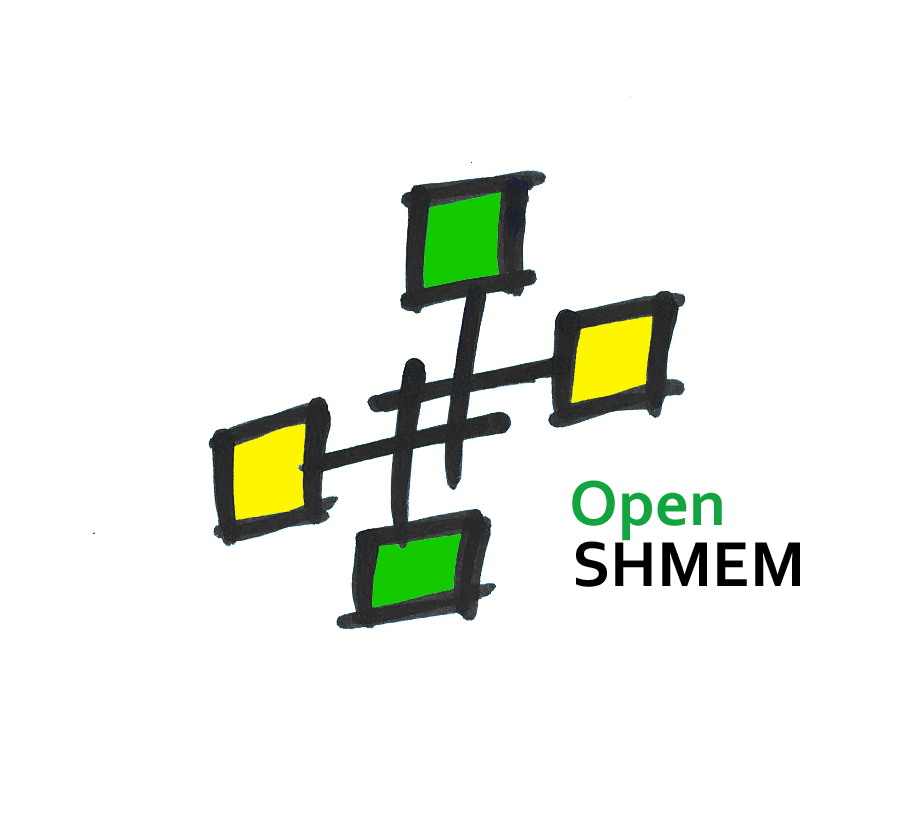
\includegraphics[scale=0.65]{figures/OpenSHMEM_Pound}\\
\url{http://www.openshmem.org/}
\par
\end{center}

\begin{center}
Version \insertDocVersion
\par
\end{center}

\vspace{0.5in}
\begin{center}
\today
\end{center}

\vspace{0.5in}

\vfill{}

\section*{Development by}
\begin{itemize}
\item For a current list of contributors and collaborators please see\\
  \url{http://www.openshmem.org/site/Contributors/}
\item For a current list of OpenSHMEM implementations and tools, please see\\
  \url{http://openshmem.org/site/Links#impl/}

\end{itemize}

\pagebreak{}

\section*{Sponsored by}
\begin{itemize}
\item \ac{DoD}\\
  \url{http://www.defense.gov/ }
\item \ac{ORNL}\\
  \url{http://www.ornl.gov/}
\item \ac{LANL}\\
  \url{http://www.lanl.gov/}
\end{itemize}

\section*{Current Authors and Collaborators}
\begin{itemize}
\item Matthew Baker, \ac{ORNL}
\item Swen Boehm, \ac{ORNL}
\item Aurelien Bouteiller, \ac{UTK}
\item Barbara Chapman, \ac{SBU}
\item Robert Cernohous, \ac{HPE}
\item James Culhane, \ac{LANL}
\item Tony Curtis, \ac{SBU}
\item James Dinan, Intel
\item Mike Dubman, Mellanox
\item Manjunath Gorentla Venkata, \ac{ORNL}
\item Megan Grodowitz, Arm Inc.
\item Max Grossman, Rice University
\item Khaled Hamidouche, \ac{AMD}
\item Jeff Hammond, Intel
\item Yossi Itigin, Mellanox
\item Bryant Lam, \ac{DoD}
\item Akhil Langer, NVIDIA
\item Jeff Kuehn, \ac{LANL}
\item Jens Manser, \ac{DoD}
\item Tiffany M. Mintz, \ac{ORNL}
\item David Ozog, Intel
\item Nicholas Park, \ac{DoD}
\item Steve Poole, \ac{OSSS}
\item Wendy Poole, \ac{OSSS}
\item Swaroop Pophale, \ac{ORNL}
\item Sreeram Potluri, NVIDIA
\item Howard Pritchard, \ac{LANL}
\item Md. Wasi-ur- Rahman, Intel
\item Naveen Ravichandrasekaran, \ac{HPE}
\item Michael Raymond, \ac{HPE}
\item James Ross, \ac{ARL}
\item Pavel Shamis, Arm Inc.
\item Sameer Shende, \ac{UO}
\item Min Si, \ac{ANL}
\item Lauren Smith, \ac{DoD}

\end{itemize}

\section*{Alumni Authors and Collaborators}
\begin{itemize}
\item Amrita Banerjee, \ac{UH}
\item Monika ten Bruggencate, Cray Inc.
\item Eduardo D'Azevedo, \ac{ORNL}
\item Karl Feind, \ac{Altair}
\item Oscar Hernandez, \ac{ORNL}
\item David Knaak, Cray Inc.
\item Gregory Koenig, \ac{ORNL}
\item Graham Lopez, \ac{ORNL}
\item Ricardo Mauricio, \ac{UH}
\item Ram Nanjegowda, \ac{UH}
\item Aaron Welch, \ac{ORNL}

\end{itemize}

\date{\today}

\section*{Acknowledgments}
The \openshmem specification belongs to Open Source Software Solutions, Inc.
(OSSS), a non-profit organization, under an agreement with HPE. For a current list
of Contributors and Collaborators, please see
  \url{http://www.openshmem.org/site/Contributors/}.
We gratefully acknowledge support from
Oak Ridge National Laboratory's
Extreme Scale Systems Center and the continuing support of the Department of Defense.\\
\\
We would also like to acknowledge the contribution of the members of the
\openshmem mailing list for their ideas, discussions, suggestions, and
constructive criticism which has helped us improve this document.\\
\\
\openshmem[1.4] is dedicated to the memory of David Charles Knaak. David was a highly involved
colleague and contributor to the entire OpenSHMEM project. He will be missed.


\setcounter{tocdepth}{4}
\setcounter{secnumdepth}{4}
\tableofcontents

\mainmatter  % included for use of documenttype 'book'

% Set header/footer for main content
\pagestyle{fancy}   %replacing {headings} with {fancy} for customization
\fancyhf{}
\fancyhead[L]{\leftmark}
\fancyhead[R]{\thepage}
\renewcommand{\headrulewidth}{0pt}
\let\thesectionOrig\thesection % Used by backmatter to restore Annex numbering.
\renewcommand{\thesection}{\arabic{section}}

{ %using setlength to force standardized spacing, if needed
% this command is ended in backmatter.tex
%\setlength{\baselineskip}{3pt plus 3pt minus 3pt}

\setlength{\parskip}{3pt}




\section{The OpenSHMEM Effort}\label{subsec:openshmem_effort}
\openshmem is a \ac{PGAS} library interface specification. \openshmem aims to
provide a standard \ac{API} for SHMEM libraries to aid portability and
facilitate uniform predictable results of \openshmem programs by explicitly
stating the behavior and semantics of the \openshmem library calls. Through the
different versions, \openshmem will continue to address the requirements of the
\ac{PGAS} community.  As of this specification, existing vendors are moving
towards \openshmem compliant implementations and new vendors are developing
\openshmem library implementations to help the users write portable \openshmem
code. This ensures that programs can run on multiple platforms without having to
deal with subtle vendor-specific implementation differences. For more details on
the history of \openshmem please refer to the
\hyperref[sec:openshmem_history]{History of \openshmem} section.  

The \openshmem\footnote{The \openshmem specification is owned by Open Source
Software Solutions Inc., a non-profit organization, under an agreement with
\ac{HPE}.} effort is driven by the \ac{DoD} with continuous input from the \openshmem community.
To see all of the contributors and participants for the \openshmem API,
please see: \url{http://www.openshmem.org/site/Contributors}. In addition to the
specification, the effort includes a reference \openshmem
implementation, validation and verification suites, tools, a mailing list and
website infrastructure to support specification activities. For more information
please refer to: \url{http://www.openshmem.org/}.


\section{Programming Model Overview}\label{subsec:programming_model}
\openshmem implements \ac{PGAS} by defining remotely accessible data objects as
mechanisms to share information among \openshmem processes or \acp{PE} and
private data objects that are accessible by the \ac{PE} itself. The \ac{API}
allows communication and synchronization operations on both private (local to
the PE initiating the operation) and remotely accessible data objects. The key
feature of \openshmem is that data transfer operations are
\textit{\textbf{one-sided}} in nature. This means that a local \ac{PE} executing
a data transfer routine does not require the participation of the remote \ac{PE}
to complete the routine. This allows for overlap between communication and
computation to hide data transfer latencies, which makes  \openshmem ideal for
unstructured, small/medium size data communication patterns. The \openshmem
library routines have the potential to provide a low-latency, high-bandwidth
communication \ac{API} for use in highly parallelized scalable programs.  

The \openshmem{} interfaces can be used to implement \ac{SPMD} style programs.
It provides interfaces to start the \openshmem{} \ac{PE}s in parallel, and
communication and synchronization interfaces to access remotely accessible data
objects across \ac{PE}s. These interfaces can be leveraged to divide a problem
into multiple sub-problems that can be solved independently or with coordination
using the communication and synchronization interfaces.  The \openshmem
specification defines library calls, constants, variables, and language bindings
for \Clang{} and \Fortran{}.  The \Cpp{} interface is currently the same as that
for \Clang. Unlike UPC, Fortran 2008, Titanium, X10 and Chapel, which are all
PGAS languages, \openshmem relies on the user to use the library calls  to
implement the correct semantics of its programming model.

An overview of the \openshmem routines is described below:

\begin{enumerate}

\item \textbf{Library Setup and Query}
\begin{enumerate}
  \item \OPR{Initialization}: The \openshmem library environment is initialized. 
  \item \OPR{Query}: The local \ac{PE} may get number of \acp{PE} running the same
      program and its unique integer identifier. 
  \item \OPR{Accessibility}: The local \ac{PE} can find out if a remote \ac{PE} is
      executing the same binary, or if a particular symmetric data object can be
      accessed by a remote \ac{PE}, or may obtain a pointer to a symmetric data
      object on the specified remote \ac{PE} on shared memory systems.
\end{enumerate}

\item \textbf{Symmetric Data Object Management}
\begin{enumerate}
  \item \OPR{Allocation}: All executing \ac{PE}s must participate in the
      allocation of a symmetric data object with identical arguments.
  \item  \OPR{Deallocation}: All executing \ac{PE}s must participate in the
      deallocation of the same symmetric data object with identical arguments.
  \item  \OPR{Reallocation}: All executing \ac{PE}s must participate in the
      reallocation of the same symmetric data object with identical arguments.
\end{enumerate}

\item \textbf{Remote Memory Access}
\begin{enumerate}
    \item \PUT: The local \ac{PE} specifies the \source{} data object (private
        or symmetric) that is copied to the symmetric data object on the remote
        \ac{PE}. 
  \item \GET: The local \ac{PE} specifies the symmetric data object on the remote
      \ac{PE} that is copied to a data object (private or symmetric) on the local
      \ac{PE}. 
\end{enumerate}

\item \textbf{Atomics}
\begin{enumerate}
    \item \OPR{Swap}: The \ac{PE} initiating the swap gets the old value of a
        symmetric data object from a remote \ac{PE} and copies a new value to
        that symmetric data object on the remote \ac{PE}.
  \item \OPR{Increment}: The \ac{PE} initiating the increment adds 1 to the
      symmetric data object on the remote \ac{PE}.
  \item \OPR{Add}: The \ac{PE} initiating the add specifies the value to be added
      to the symmetric data object on the remote \ac{PE}.
  \item \OPR{Compare and Swap}: The \ac{PE} initiating the swap gets the old value
      of the symmetric data object based on a value to be compared and copies a
      new value to the symmetric data object on the remote \ac{PE}.
  \item \OPR{Fetch and Increment}: The \ac{PE} initiating the increment adds 1 to
      the symmetric data object on the remote \ac{PE} and returns with the old
      value.
  \item \OPR{Fetch and Add}: The \ac{PE} initiating the add specifies the value to
      be added to the symmetric data object on the remote \ac{PE} and returns with
      the old value.
\end{enumerate}

\item \textbf{Synchronization and Ordering}
\begin{enumerate}
  \item \OPR{Fence}: The \ac{PE} calling fence ensures ordering of remote access
      operations and stores to symmetric data objects with respect to a specific
      destination \ac{PE}. 
  \item \OPR{Quiet}: The \ac{PE} calling quiet ensures completion of remote access
      operations and stores to symmetric data objects. 
  \item \OPR{Barrier}: All or some \ac{PE}s collectively synchronize and ensure
      completion of all remote and local updates prior to any \ac{PE} returning
      from the call.
\end{enumerate}

\item \textbf{Collective Communication}
\begin{enumerate}
  \item \OPR{Broadcast}: The \textit{root} \ac{PE} specifies a symmetric data
      object to be copied to a symmetric data object on one or more remote
      \acp{PE} (not including itself). 
  \item \OPR{Collection}: All \acp{PE} participating in the routine get the result
      of concatenated symmetric objects contributed by each of the \acp{PE} in
      another symmetric data object.
  \item \OPR{Reduction}: All \acp{PE} participating in the routine get the result
      of an associative binary routine over elements of the specified symmetric
      data object on another symmetric data object. 
\end{enumerate}

\item \textbf{Mutual Exclusion}
\begin{enumerate}
  \item \OPR{Set Lock}: The \ac{PE} acquires exclusive access to the region
      bounded by the symmetric \textit{lock} variable.
  \item \OPR{Test Lock}: The \ac{PE} tests the symmetric \textit{lock} variable
      for availability.
  \item \OPR{Clear Lock}: The \ac{PE} which has previously acquired the
      \textit{lock} releases it.
\end{enumerate}

\item \textbf{Data Cache Control \textit{(deprecated on cache coherent systems)}}
\begin{enumerate}
  \item Implementation of mechanisms to exploit the capabilities of hardware cache
      if available.
\end{enumerate}
\end{enumerate}


\section{Memory Model}\label{subsec:memory_model}
\begin{figure}[h]
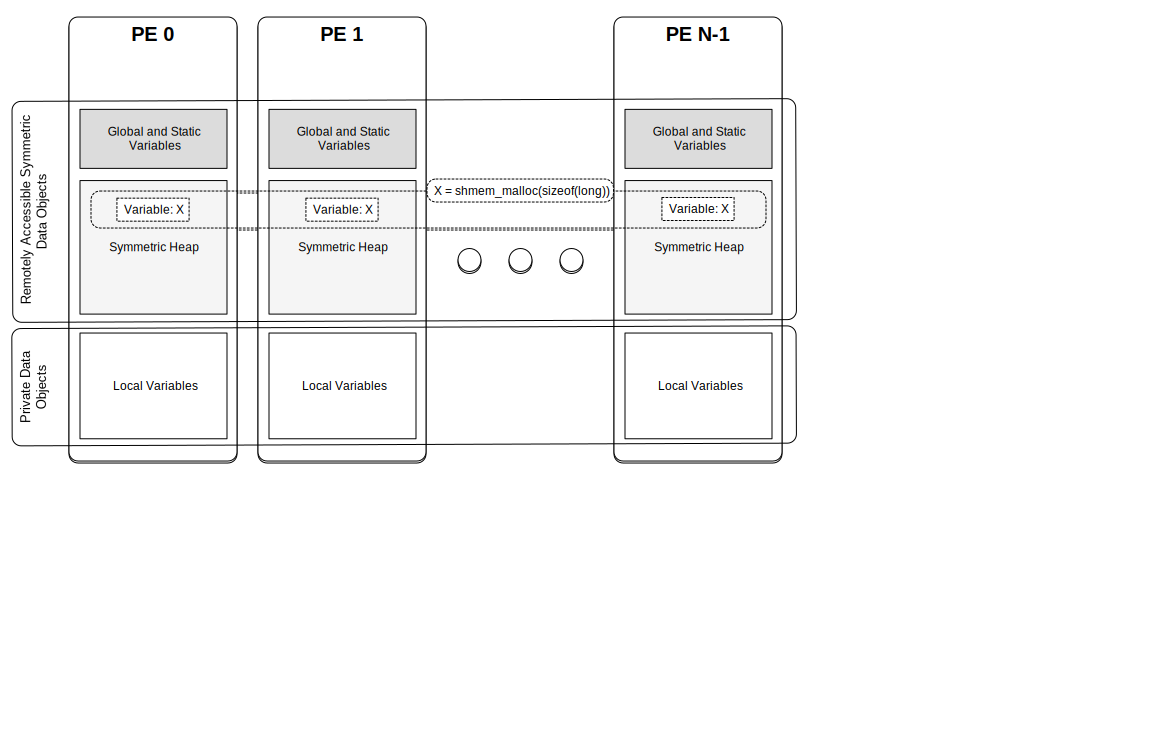
\includegraphics[width=0.95\textwidth]{figures/mem_model}      
\caption{\openshmem Memory Model}
\label{fig:mem_model}                                               
\end{figure}      
%
An \openshmem program consists of data objects that are private to each \ac{PE}
and data  objects that are remotely accessible by all \acp{PE}. Private data
objects are stored in the local memory of each \ac{PE} and can only be accessed
by the \ac{PE} itself; these data objects cannot be accessed by other \acp{PE}
via \openshmem routines. Private data objects follow the memory model of
\Cstd or \Fortran. Remotely accessible objects, however, can be accessed by
remote \acp{PE} using \openshmem routines.  Remotely accessible data objects are
called \emph{Symmetric Data Objects}.  Each symmetric data object has a
corresponding object with the same name, type, and size on all \acp{PE} where that object is
accessible via the \openshmem \ac{API}\footnote{For efficiency reasons,
the same offset (from an arbitrary memory address) for symmetric data
objects might be used on all \acp{PE}. Further discussion about symmetric heap
layout and implementation efficiency can be found in section
\ref{subsec:shfree}}.  (For the definition of what is accessible, see the
descriptions for \FUNC{shmem\_pe\_accessible} and \FUNC{shmem\_addr\_accessible}
in sections \ref{subsec:shmem_pe_accessible} and
\ref{subsec:shmem_addr_accessible}.) Symmetric data objects accessed via typed
\openshmem interfaces are required to be naturally aligned based on their type
requirements and underlying architecture.  In \openshmem the following kinds of
data objects are symmetric:
%
\begin{itemize}
\item
  \begin{deprecate}
    \Fortran data objects in common blocks or with the \CTYPE{SAVE} attribute.
    These data objects must not be defined in a dynamic shared object (DSO).
  \end{deprecate}
\item Global and static \Cstd and \Cpp variables. These data objects must
  not  be defined in a DSO.
\item
  \begin{deprecate}
    \Fortran arrays allocated with \FUNC{shpalloc}
  \end{deprecate}
\item \Cstd and \Cpp data allocated by \openshmem memory management routines
  (Section~\ref{sec:memory_management})
\end{itemize}       

\openshmem dynamic memory allocation routines (\FUNC{shpalloc} and
\FUNC{shmem\_malloc}) allow collective allocation of \emph{Symmetric Data
Objects} on a special memory region called the \emph{Symmetric Heap}. The
Symmetric Heap is created during the execution of a program at a memory location
determined by the implementation. The Symmetric Heap may reside in different
memory regions on different \acp{PE}. Figure~\ref{fig:mem_model} shows how
\openshmem implements a \ac{PGAS} model using remotely accessible symmetric
objects and private data objects when executing an \openshmem program.
Symmetric data objects are stored on the symmetric heap or in the global/static
memory section of each \ac{PE}. 


\section{Execution Model}\label{subsec:execution_model}
An \openshmem program consists of a set of \openshmem processes called
\acp{PE}.  While not required by \openshmem, in typical usage, \acp{PE} are
executed using a single program, multiple data (\ac{SPMD}) model.  \ac{SPMD}
requires each \ac{PE} to use the same executable; however, \acp{PE} are able to
follow divergent control paths.  \acp{PE} are often implemented using \ac{OS}
processes and \acp{PE} are permitted to create additional
threads, when supported by the \openshmem library.

\ac{PE} execution is loosely coupled, relying on \openshmem operations to
communicate and synchronize among executing \acp{PE}.  The \openshmem phase in
a program begins with a call to the initialization routine \FUNC{shmem\_init}
or \FUNC{shmem\_init\_thread}, which must be performed before using any of the
other \openshmem library routines. 
An \openshmem program concludes its use of the \openshmem library when all \acp{PE} call
\FUNC{shmem\_finalize} or any \ac{PE} calls \FUNC{shmem\_global\_exit}.
During a call to \FUNC{shmem\_finalize}, the \openshmem library must
complete all pending communication and release all the resources associated to
the library using an implicit collective synchronization across \acp{PE}.
Calling any \openshmem routine before initialization or after
\FUNC{shmem\_finalize} leads to undefined behavior. After finalization, a
subsequent initialization call also leads to undefined behavior.

The \acp{PE} of the \openshmem program are identified by unique integers.  The
identifiers are integers assigned in a monotonically increasing manner from zero
to one less than the total number of \acp{PE}. \ac{PE} identifiers are used for
\openshmem calls (e.g., to specify \OPR{put} or \OPR{get} routines on symmetric
data objects, collective synchronization calls) or to dictate a control flow for
\acp{PE} using constructs of \Cstd. The identifiers are fixed for
the duration of the \openshmem phase of a program.

\subsection{Progress of OpenSHMEM Operations}\label{subsec:progress}

The \openshmem model assumes that computation and communication are naturally
overlapped. \openshmem programs are expected to exhibit progression of
communication both with and without \openshmem calls. For point-to-point
operations, consider a \ac{PE} that is
engaged in a computation with no \openshmem calls. Other \acp{PE} should be able
to communicate (e.g., \OPR{put}, \OPR{get}, \OPR{atomic}, etc.) and
complete communication operations with that computationally-bound \ac{PE}
without that \ac{PE} issuing any explicit \openshmem calls. One-sided \openshmem
communication calls involving that \ac{PE} should progress regardless of when
that \ac{PE} next engages in an \openshmem call. Similarly,
for non-blocking collectives, consider the \acp{PE} that are part of a team
issuing a non-blocking collective and overlapping collective completion with
computation. Once a non-blocking collective operation is initiated by
all of the \acp{PE} in the team of the collective, any \ac{PE} in the team must
eventually observe completion through a call to \FUNC{shmem\_req\_test} or a
call to \FUNC{shmem\_req\_wait}.

\parimpnotes{
  An \openshmem implementation for hardware that does not provide
  asynchronous communication capabilities may require a software progress
  thread in order to process remotely-issued communication requests without
  explicit program calls to the \openshmem library.

  High performance implementations of \openshmem are expected to leverage
  hardware offload capabilities and provide asynchronous one-sided
  communication without software assistance.

  Implementations should avoid deferring the execution of one-sided
  operations until a synchronization point where data is known to be
  available. High-quality implementations should attempt asynchronous delivery
  whenever possible, for performance reasons. Additionally, the \openshmem
  community discourages releasing \openshmem implementations that do not
  provide asynchronous one-sided operations, as these have very limited
  performance value for \openshmem programs.
}

\subsection{Invoking OpenSHMEM Operations}\label{subsec:invoking_openshmem_operations}

Pointer arguments to \openshmem routines that point to non-\CTYPE{const} data must not
overlap in memory with other arguments to the same \openshmem operation, with
the exception of in-place reductions as described in Section~\ref{subsec:shmem_reductions}.
Otherwise, the behavior is undefined.  Two arguments overlap in memory if any
of their data elements are contained in the same physical memory locations.
For example, consider an address $a$ returned by the \FUNC{shmem\_ptr} operation
for symmetric object $A$ on \ac{PE} $i$.  Providing the local address $a$ and
the symmetric address of object $A$ to an \openshmem operation targeting
\ac{PE} $i$ results in undefined behavior.

Buffers provided to \openshmem routines are \emph{in-use} until the
corresponding \openshmem operation has completed at the calling \ac{PE}.
Updates to a buffer that is in-use, including updates performed through locally
and remotely issued \openshmem operations, result in undefined behavior.
Similarly, reads from a buffer that is in-use are allowed only when the buffer
was provided as a \CTYPE{const}-qualified argument to the \openshmem routine for
which it is in-use.  Otherwise, the behavior is undefined. Exceptions are made for
buffers that are in-use by \acp{AMO}, as described in
Section~\ref{subsec:amo_guarantees}. For information regarding the completion
of \openshmem operations, see Section~\ref{subsec:memory_order}.

\openshmem routines with multiple symmetric object arguments do not require
these symmetric objects to be located within the same symmetric memory segment.
For example, objects located in the symmetric data segment and objects located
in the symmetric heap can be provided as arguments to the same \openshmem
operation.


\section{Language Bindings and Conformance}\label{subsec:bindings}
\openshmem provides ISO \Clang{} and \Fortran{} \textit{90} language bindings.
Any implementation that provides both \Clang{} and \Fortran{} bindings can claim
conformance to the specification. An implementation that provides e.g.\ only a
\Clang{} interface may claim to conform to the \openshmem specification with
respect to the \Clang{} language, but not to \Fortran, and should make this
clear in its documentation. The \openshmem header files for \Clang{} and
\Fortran{} must contain only the interfaces and constant names defined in this
specification.

\openshmem \ac{API}s can be implemented as either routines or macros. However,
implementing the interfaces using macros is strongly discouraged as this could
severely limit the use of external profiling tools and high-level compiler
optimizations. An \openshmem program should avoid defining routine names,
variables, or identifiers with the prefix \shmemprefix (for \Clang{} and
\Fortran), \shmemprefixC (for \Clang) or with \openshmem \ac{API} names.

All \openshmem extension \ac{API}s that are not part of this specification must
be defined in the \FUNC{shmemx.h} include file. These extensions shall use the
\FUNC{shmemx\_} prefix for all routine, variable, and constant names.


\section{Library Constants}\label{subsec:library_constants}
The \openshmem library provides a set of compile-time constants that may
be used to specify options to API routines, provide implementation-specific
parameters, or return information about the implementation.
All constants that start with \CONST{\_SHMEM\_*} are deprecated,
but provided for backwards compatibility.

\begin{longtable}{|p{0.45\textwidth}|p{0.5\textwidth}|}
\hline
\textbf{Constant} & \textbf{Description}
\tabularnewline \hline
\endhead
%%
\LibConstDecl[\CorCpp]{SHMEM\_THREAD\_SINGLE} &
The \openshmem thread support level which specifies that the program
may not be multithreaded.
See Section~\ref{subsec:thread_support} for more detail about its use.
\tabularnewline \hline
%%
\LibConstDecl[\CorCpp]{SHMEM\_THREAD\_FUNNELED} &
The \openshmem thread support level which specifies that the program
may be multithreaded but must ensure that only the main thread invokes
the \openshmem interfaces.
See Section~\ref{subsec:thread_support} for more detail about its use.
\tabularnewline \hline
%%
\LibConstDecl[\CorCpp]{SHMEM\_THREAD\_SERIALIZED} &
The \openshmem thread support level which specifies that the program
may be multithreaded but must ensure that the \openshmem interfaces
are not invoked concurrently by multiple threads.
See Section~\ref{subsec:thread_support} for more detail about its use.
\tabularnewline \hline
%%
\LibConstDecl[\CorCpp]{SHMEM\_THREAD\_MULTIPLE} &
The \openshmem thread support level which specifies that the program
may be multithreaded and any thread may invoke the \openshmem interfaces.
See Section~\ref{subsec:thread_support} for more detail about its use.
\tabularnewline \hline
%%
\LibConstDecl[\CorCpp]{SHMEM\_CTX\_DEFAULT} &
Handle of type \CTYPE{shmem\_ctx\_t} that corresponds to the
default communication context.  All point-to-point communication operations
and synchronizations that do not specify a context are performed on the
default context.
See Section~\ref{sec:ctx} for more detail about its use.
\tabularnewline \hline
%%
\LibConstDecl[\CorCpp]{SHMEM\_CTX\_SERIALIZE} &
The context creation option which specifies that the given context
is shareable but will not be used by multiple threads concurrently.
See Section~\ref{subsec:shmem_ctx_create} for more detail about its use.
\tabularnewline \hline
%%
\LibConstDecl[\CorCpp]{SHMEM\_CTX\_PRIVATE} &
The context creation option which specifies that the given context
will be used only by the thread that created it.
See Section~\ref{subsec:shmem_ctx_create} for more detail about its use.
\tabularnewline \hline
%%
\LibConstDecl[\CorCpp]{SHMEM\_CTX\_NOSTORE} &
The context creation option which specifies that quiet and fence operations
performed on the given context are not required to enforce completion and
ordering of memory store operations.
See Section~\ref{subsec:shmem_ctx_create} for more detail about its use.
\tabularnewline \hline
%%
\LibConstDecl{SHMEM\_SYNC\_VALUE}
\begin{DeprecateBlock}
  \LibConstDecl[\CorCpp]{\_SHMEM\_SYNC\_VALUE}
\end{DeprecateBlock}
&
The value used to initialize the elements of \VAR{pSync} arrays.
The value of this constant is implementation specific.
See Section~\ref{subsec:coll} for more detail about its use.
\tabularnewline \hline
%%
\LibConstDecl{SHMEM\_SYNC\_SIZE} &
Length of a work array that can be used with any SHMEM collective
communication operation.
Work arrays sized for specific operations may consume less memory.
The value of this constant is implementation specific.
See Section~\ref{subsec:coll} for more detail about its use.
\tabularnewline \hline
%%
\LibConstDecl{SHMEM\_BCAST\_SYNC\_SIZE}
\begin{DeprecateBlock}
  \LibConstDecl[\CorCpp]{\_SHMEM\_BCAST\_SYNC\_SIZE}
\end{DeprecateBlock}
&
Length of the \VAR{pSync} arrays needed for broadcast routines. The value
of this constant is implementation specific.
See Section~\ref{subsec:shmem_broadcast} for more detail about its use.
\tabularnewline \hline
%%
\LibConstDecl{SHMEM\_REDUCE\_SYNC\_SIZE}
\begin{DeprecateBlock}
  \LibConstDecl[\CorCpp]{\_SHMEM\_REDUCE\_SYNC\_SIZE}
\end{DeprecateBlock}
&
Length of the work arrays needed for reduction routines.
The value of this constant is implementation specific.
See Section~\ref{subsec:shmem_reductions} for more detail about its use.
\tabularnewline \hline
%%
\LibConstDecl{SHMEM\_BARRIER\_SYNC\_SIZE}
\begin{DeprecateBlock}
  \LibConstDecl[\CorCpp]{\_SHMEM\_BARRIER\_SYNC\_SIZE}
\end{DeprecateBlock}
&
Length of the work array needed for barrier routines.
The value of this constant is implementation specific.
See Section~\ref{subsec:shmem_barrier} for more detail about its use.

\tabularnewline \hline
%%
\LibConstDecl{SHMEM\_COLLECT\_SYNC\_SIZE}
\begin{DeprecateBlock}
  \LibConstDecl[\CorCpp]{\_SHMEM\_COLLECT\_SYNC\_SIZE}
\end{DeprecateBlock}
&
Length of the work array needed for collect routines.
The value of this constant is implementation specific.
See Section~\ref{subsec:shmem_collect} for more detail about its use.
\tabularnewline \hline
%%
\LibConstDecl{SHMEM\_ALLTOALL\_SYNC\_SIZE} &
Length of the work array needed for \FUNC{shmem\_alltoall} routines.
The value of this constant is implementation specific.
See Section~\ref{subsec:shmem_alltoall} for more detail about its use.
\tabularnewline \hline
%%
\LibConstDecl{SHMEM\_ALLTOALLS\_SYNC\_SIZE} &
Length of the work array needed for \FUNC{shmem\_alltoalls} routines.
The value of this constant is implementation specific.
See Section~\ref{subsec:shmem_alltoalls} for more detail about its use.
\tabularnewline \hline
%%
\LibConstDecl{SHMEM\_REDUCE\_MIN\_WRKDATA\_SIZE}
\begin{DeprecateBlock}
  \LibConstDecl[\CorCpp]{\_SHMEM\_REDUCE\_MIN\_WRKDATA\_SIZE}
\end{DeprecateBlock}
&
Minimum length of work arrays used in various collective routines.
\tabularnewline \hline
%%
\LibConstDecl{SHMEM\_MAJOR\_VERSION}
\begin{DeprecateBlock}
  \LibConstDecl[\CorCpp]{\_SHMEM\_MAJOR\_VERSION}
\end{DeprecateBlock}
&
Integer representing the major version of \openshmem standard in use.
\tabularnewline \hline
%%
\LibConstDecl{SHMEM\_MINOR\_VERSION}
\begin{DeprecateBlock}
  \LibConstDecl[\CorCpp]{\_SHMEM\_MINOR\_VERSION}
\end{DeprecateBlock}
&
Integer representing the minor version of \openshmem standard in use.
\tabularnewline \hline
%%
\LibConstDecl{SHMEM\_MAX\_NAME\_LEN}
\begin{DeprecateBlock}
  \LibConstDecl[\CorCpp]{\_SHMEM\_MAX\_NAME\_LEN}
\end{DeprecateBlock}
&
Integer representing the maximum length of \CONST{SHMEM\_VENDOR\_STRING}.
\tabularnewline \hline
%%
\LibConstDecl{SHMEM\_VENDOR\_STRING}
\begin{DeprecateBlock}
  \LibConstDecl[\CorCpp]{\_SHMEM\_VENDOR\_STRING}
\end{DeprecateBlock}
&
String representing vendor defined information of size at most
\CONST{SHMEM\_MAX\_NAME\_LEN}.
In \CorCpp{}, the string is terminated by a null character.  In \Fortran, the
string of size less than \CONST{SHMEM\_MAX\_NAME\_LEN} is padded with blank
characters up to size \CONST{SHMEM\_MAX\_NAME\_LEN}.
\tabularnewline \hline
%%
\LibConstDecl{SHMEM\_CMP\_EQ}
\begin{DeprecateBlock}
  \LibConstDecl[\CorCpp]{\_SHMEM\_CMP\_EQ}
\end{DeprecateBlock}
&
An integer constant expression corresponding to the
``equal to'' comparison operation.
See Section~\ref{subsec:p2p_intro} for more detail about its use.
\tabularnewline \hline
%%
\LibConstDecl{SHMEM\_CMP\_NE}
\begin{DeprecateBlock}
  \LibConstDecl[\CorCpp]{\_SHMEM\_CMP\_NEEQ}
\end{DeprecateBlock}
&
An integer constant expression corresponding to the
``not equal to'' comparison operation.
See Section~\ref{subsec:p2p_intro} for more detail about its use.
\tabularnewline \hline
%%
\LibConstDecl{SHMEM\_CMP\_LT}
\begin{DeprecateBlock}
  \LibConstDecl[\CorCpp]{\_SHMEM\_CMP\_LT}
\end{DeprecateBlock}
&
An integer constant expression corresponding to the
``less than'' comparison operation.
See Section~\ref{subsec:p2p_intro} for more detail about its use.
\tabularnewline \hline
%%
\LibConstDecl{SHMEM\_CMP\_LE}
\begin{DeprecateBlock}
  \LibConstDecl[\CorCpp]{\_SHMEM\_CMP\_LE}
\end{DeprecateBlock}
&
An integer constant expression corresponding to the
``less than or equal to'' comparison operation.
See Section~\ref{subsec:p2p_intro} for more detail about its use.
\tabularnewline \hline
%%
\LibConstDecl{SHMEM\_CMP\_GT}
\begin{DeprecateBlock}
  \LibConstDecl[\CorCpp]{\_SHMEM\_CMP\_GT}
\end{DeprecateBlock}
&
An integer constant expression corresponding to the
``greater than'' comparison operation.
See Section~\ref{subsec:p2p_intro} for more detail about its use.
\tabularnewline \hline
%%
\LibConstDecl{SHMEM\_CMP\_GE}
\begin{DeprecateBlock}
  \LibConstDecl[\CorCpp]{\_SHMEM\_CMP\_GE}
\end{DeprecateBlock}
&
An integer constant expression corresponding to the
``greater than or equal to'' comparison operation.
See Section~\ref{subsec:p2p_intro} for more detail about its use.
\tabularnewline \hline
%%
\end{longtable}


\section{Library Handles}\label{subsec:library_handles}
\TableIndex{Library Handles}
\TableIndex{Handles}

The \openshmem library provides a set of predefined named constant handles.
All named constants can be used in initialization expressions or assignments,
but not necessarily in array declarations or as labels in \Cstd switch statements.
This implies named constants to be link-time but not necessarily compile-time
constants.

\begin{longtable}{|p{0.45\textwidth}|p{0.5\textwidth}|}
\hline
\textbf{Handle} & \textbf{Description}
\tabularnewline \hline
\endhead
%%
\color{Green}
\LibHandleDecl{SHMEM\_TEAM\_WORLD} &
\color{Green}
Handle of type \CTYPE{shmem\_team\_t} that corresponds to the
default team of all \acp{PE} in the \openshmem program.  All point-to-point
communication operations and synchronizations that do not specify a team
are performed on the default team.
See Section~\ref{subsec:team} for more detail about its use.
\tabularnewline \hline
%%
\color{Green}
\LibHandleDecl{SHMEM\_TEAM\_NODE} &
\color{Green}
Handle of type \CTYPE{shmem\_team\_t} that corresponds a team of \acp{PE}
which share node level resources, such as shared memory, network
interfaces, etc. When this handle is used by some \ac{PE}, it will refer
to the node level team containing that \ac{PE}.
See Section~\ref{subsec:team} for more detail about its use.
\tabularnewline \hline
%%
\LibHandleDecl{SHMEM\_CTX\_DEFAULT} &
Handle of type \CTYPE{shmem\_ctx\_t} that corresponds to the
default communication context.  All point-to-point communication operations
and synchronizations that do not specify a context are performed on the
default context.
See Section~\ref{sec:ctx} for more detail about its use.
\tabularnewline \hline
%%
\end{longtable}


\section{Environment Variables }\label{subsec:environment_variables}
The \openshmem specification provides a set of environment variables that allows
users to configure the \openshmem implementation, and receive information about
the implementation. The implementations of the specification are free to define
additional variables. Currently, the specification defines four environment
variables.

\medskip{}

\begin{tabular}{|l|l|l|}
\hline 
Variable & Value & Routine\tabularnewline
\hline 
\hline 
\texttt{SMA\_VERSION} & any & print the library version at
start-up\tabularnewline
\hline 
\texttt{SMA\_INFO} & any & print helpful text about all these environment
variables\tabularnewline
\hline 
\texttt{SMA\_SYMMETRIC\_SIZE} & non-negative integer & number of bytes to
allocate for symmetric heap\tabularnewline
\hline 
\texttt{SMA\_DEBUG} & any & enable debugging messages\tabularnewline
\hline 
\end{tabular}

\medskip{}


\clearpage



\section{OpenSHMEM Library \acs{API}}\label{sec:openshmem_library_api}

\subsection{Library Setup, Exit, and Query Routines}
The library setup and query interfaces that initialize and monitor the parallel
environment of the \acp{PE}.

\subsubsection{\textbf{SHMEM\_INIT}}\label{subsec:shmem_init}
\apisummary{
    A collective operation that allocates and initializes the resources used by
    the \openshmem library.
}

\begin{apidefinition}

\begin{Csynopsis}
void shmem_init(void);
\end{Csynopsis}

\begin{Fsynopsis}
CALL SHMEM_INIT()
\end{Fsynopsis}


\begin{apiarguments}
    \apiargument{None.}{}{}
\end{apiarguments}

\apidescription{
    \FUNC{shmem\_init} allocates and initializes resources used by the \openshmem
    library. It is a collective operation that all \acp{PE} must call before any
    other \openshmem routine may be called. At the end of the \openshmem program
    which it initialized, the call to \FUNC{shmem\_init} must be matched with a
    call to \FUNC{shmem\_finalize}. After a single call to \FUNC{shmem\_init}, a
    subsequent call to \FUNC{shmem\_init} in the same program results in undefined
    behavior.
}

\apireturnvalues{
    None.
}      

\apinotes{
    As of \openshmem Specification 1.2 the use of \FUNC{start\_pes} has been
    deprecated and is replaced with \FUNC{shmem\_init}. While support for
    \FUNC{start\_pes} is still required in \openshmem libraries, users are
    encouraged to use \FUNC{shmem\_init}. Replacing \FUNC{start\_pes} with
    \FUNC{shmem\_init} in \openshmem programs with no further changes is possible;
    there is an implicit \FUNC{shmem\_finalize} at the end of main.  However,
    \FUNC{shmem\_init} differs slightly from \FUNC{start\_pes}: multiple calls to
    \FUNC{shmem\_init} within a program results in undefined behavior, while in the
    case of \FUNC{start\_pes}, any subsequent calls to \FUNC{start\_pes} after the
    first one resulted in a no-op.
}

\begin{apiexamples}

\apifexample
    { This is a simple program that calls \FUNC{shmem\_init}: } 
    { example_code/shmem_init_example.f90 }
    {}

\end{apiexamples}

\end{apidefinition}


\subsubsection{\textbf{SHMEM\_MY\_PE}}\label{subsec:shmem_my_pe}
\apisummary{
    Returns the number of the calling \ac{PE}.
}

\begin{apidefinition}

\begin{Csynopsis}
int shmem_my_pe(void);
\end{Csynopsis}

\begin{Fsynopsis}
INTEGER SHMEM_MY_PE, ME
ME = SHMEM_MY_PE()
\end{Fsynopsis}

\begin{apiarguments}
    \apiargument{None.}{}{}
\end{apiarguments}

\apidescription{
    This routine returns the \ac{PE} number of the calling \ac{PE}.  It accepts no
    arguments.  The result is an integer between \CONST{0} and \VAR{npes} -
    \CONST{1}, where \VAR{npes} is the total number of \ac{PE}s executing the
    current program.
}

\apireturnvalues{
    Integer - Between \CONST{0} and \VAR{npes} - \CONST{1}
}

\apinotes{
    Each \ac{PE} has a unique number or identifier. As of \openshmem Specification
    1.2 the use of \FUNC{\_my\_pe} has been deprecated. Although \openshmem
    libraries are required to support the call, users are encouraged to use
    \FUNC{shmem\_my\_pe} instead.  The behavior and signature  of the routine
    \FUNC{shmem\_my\_pe} remains unchanged from the deprecated \FUNC{\_my\_pe}
    version.
}

\begin{apiexamples}

\apicexample
    {The following \FUNC{shmem\_my\_pe} example is for \CorCpp{} programs:}
    {./example_code/shmem_mype_example.c}
    {}

\end{apiexamples}

\end{apidefinition}


\subsubsection{\textbf{SHMEM\_N\_PES}}\label{subsec:shmem_n_pes}
\apisummary{
    Returns the number of \ac{PE}s running in a program.
}

\begin{apidefinition}

\begin{Csynopsis}
int shmem_n_pes(void);
\end{Csynopsis}

\begin{Fsynopsis}
INTEGER SHMEM_N_PES, N_PES
N_PES = SHMEM_N_PES()
\end{Fsynopsis}

\begin{apiarguments}
    \apiargument{None.}{}{}
\end{apiarguments}

\apidescription{
    The routine returns the number of \ac{PE}s running the program.
}

\apireturnvalues{
    Integer -  Number of \ac{PE}s running the \openshmem program.
}

\apinotes{
    As of \openshmem Specification 1.2 the use of \FUNC{\_num\_pes} has been
    deprecated. Although \openshmem libraries are required to support the call,
    users are encouraged to use \FUNC{shmem\_n\_pes} instead.  The behavior and
    signature  of the routine \FUNC{shmem\_n\_pes} remains unchanged from the
    deprecated \FUNC{\_num\_pes} version.
}

\begin{apiexamples}

\apicexample
    {The following \FUNC{shmem\_n\_pes} example is for \CorCpp{} programs:}
    {./example_code/shmem_npes_example.c}
    {}

\end{apiexamples}

\end{apidefinition}


\subsubsection{\textbf{SHMEM\_FINALIZE}}\label{subsec:shmem_finalize}
\apisummary{
    A collective operation that releases resources used by the \openshmem
    library.  This only terminates the \openshmem portion of a program, not the
    entire program.
}

\begin{apidefinition}

\begin{Csynopsis}
void shmem_finalize(void);
\end{Csynopsis}

\begin{Fsynopsis}
CALL SHMEM_FINALIZE
\end{Fsynopsis}

\begin{apiarguments}
    \apiargument{None.}{}{}
\end{apiarguments}

\apidescription{
    \FUNC{shmem\_finalize} is a collective operation that ends the \openshmem
    portion of a program previously initialized by \FUNC{shmem\_init} and
    releases resources used by the \openshmem library. This collective
    operation requires all \acp{PE} to participate in the call. There is an
    implicit global barrier in \FUNC{shmem\_finalize} so that pending
    communication is completed, and no resources can be released until all
    \acp{PE} have entered \FUNC{shmem\_finalize}. \FUNC{shmem\_finalize} must be
    the last \openshmem library call encountered in the \openshmem portion of a
    program. A call to \FUNC{shmem\_finalize} will release any resources
    initialized by a corresponding call to \FUNC{shmem\_init}. All processes and
    threads that represent the \acp{PE} will still exist after the call to
    \FUNC{shmem\_finalize} returns, but they will no longer have access to any
    resources that have been released.
}

\apireturnvalues{
    None.
}

\apinotes{
    \FUNC{shmem\_finalize} releases all resources used by the \openshmem library
    including the symmetric memory heap and pointers initiated by
    \FUNC{shmem\_ptr}. This collective operation requires all \acp{PE} to
    participate in the call, not just a subset of the \acp{PE}. The
    non-\openshmem portion of a program may continue after a call to
    \FUNC{shmem\_finalize} by all \acp{PE}. There is an implicit
    \FUNC{shmem\_finalize} at the end of main, so that having an explicit call
    to \FUNC{shmem\_finalize} is optional. However, an explicit
    \FUNC{shmem\_finalize} may be required as an entry point for wrappers used
    by profiling or other tools that need to perform their own finalization.
}

\begin{apiexamples}

\apicexample
    {The following finalize example is for \CorCpp{} programs:}
    {./example_code/shmem_finalize_example.c}
    {}

\end{apiexamples}

\end{apidefinition}


\subsubsection{\textbf{SHMEM\_GLOBAL\_EXIT}}\label{subsec:shmem_global_exit}
\apisummary{
    A routine that allows any \ac{PE} to force termination of an entire program.
}

\begin{apidefinition}

\begin{Csynopsis}
void shmem_global_exit(int status);
\end{Csynopsis}

\begin{Fsynopsis}
INTEGER STATUS
CALL SHMEM_GLOBAL_EXIT(status)
\end{Fsynopsis}

\begin{apiarguments}
    \apiargument{IN}{status}{The exit status from the main program.}
\end{apiarguments}

\apidescription{
    \FUNC{shmem\_global\_exit} is a non-collective routine that allows any one
    \ac{PE} to force termination of an \openshmem program for all \acp{PE},
    passing an exit status to the execution environment. This routine terminates
    the entire program, not just the \openshmem portion.  When any \ac{PE} calls
    \FUNC{shmem\_global\_exit}, it results in the immediate notification to all
    \acp{PE} to terminate.  \FUNC{shmem\_global\_exit} flushes I/O and releases
    resources in accordance with C/C++/Fortran language requirements for normal
    program termination. If more than one \ac{PE} calls
    \FUNC{shmem\_global\_exit}, then the exit status returned to the environment
    shall be one of the values passed to \FUNC{shmem\_global\_exit} as the
    status argument.  There is no return to the caller of
    \FUNC{shmem\_global\_exit}; control is returned from the \openshmem program
    to the execution environment for all \acp{PE}.
}

\apireturnvalues{
    None.
}


\apinotes{ 
    \FUNC{shmem\_global\_exit} may be used in situations where one or more
    \acp{PE} have determined that the program has completed and/or should
    terminate early.  Accordingly, the integer status argument can be used to
    pass any information about the nature of the exit, e.g an encountered error
    or a found solution.  Since \FUNC{shmem\_global\_exit} is a non-collective
    routine, there is no implied synchronization, and all \acp{PE} must
    terminate regardless of their current execution state. While I/O must be
    flushed for standard language I/O calls from C/C++/Fortran, it is
    implementation dependent as to how I/O done by other means (e.g. third
    party I/O libraries) is handled. Similarly, resources are released
    according to C/C++/Fortran standard language requirements, but this may not
    include all resources allocated for the \openshmem program. However, a
    quality implementation will make a best effort to flush all I/O and clean
    up all resources.
}

\begin{apiexamples}

\apicexample
    {}
    {./example_code/shmem_global_exit_example.c}
    {}

\end{apiexamples}

\end{apidefinition}


\subsubsection{\textbf{SHMEM\_PE\_ACCESSIBLE}}\label{subsec:shmem_pe_accessible}
\apisummary{
    Determines whether a \ac{PE} is accessible via \openshmem's data transfer
    routines.
}

\begin{apidefinition}

\begin{Csynopsis}
int shmem_pe_accessible(int pe);
\end{Csynopsis}

\begin{Fsynopsis}
LOGICAL LOG, SHMEM_PE_ACCESSIBLE
INTEGER pe
LOG = SHMEM_PE_ACCESSIBLE(pe)
\end{Fsynopsis}

\begin{apiarguments}
    \apiargument{IN}{pe}{Specific \ac{PE} to be checked for accessibility from
    the local \ac{PE}.}
\end{apiarguments}

\apidescription{
    \FUNC{shmem\_pe\_accessible} is  a  query routine  that indicates  whether  a
    specified \ac{PE} is accessible via \openshmem from the local \ac{PE}. The
    \FUNC{shmem\_pe\_accessible} routine returns \CONST{TRUE} only if  the  remote
    \ac{PE} is a process  running from the same executable  file as the local
    \ac{PE}, indicating that full \openshmem support for symmetric data objects
    (that reside in the static memory and symmetric heap) is available, otherwise it
    returns \CONST{FALSE}.  This routine may be particularly useful for hybrid
    programming with other communication libraries (such as a \ac{MPI}) or parallel
    languages.  For example, on  SGI Altix  series  systems, \openshmem is
    supported  across multiple partitioned hosts and InfiniBand connected hosts.
    When running multiple executable MPI programs using \openshmem on an Altix, full
    \openshmem support is available between processes running from the same
    executable file. However, \openshmem support between processes of different
    executable  files  is  supported only for data objects on the symmetric heap,
    since static data objects are  not symmetric  between  different executable
    files.        
}

\apireturnvalues{
    \CorCpp: The return value is 1 if the specified \ac{PE} is a valid remote \ac{PE}
    for \openshmem routines; otherwise, it is 0.

    \Fortran: The return value is \CONST{.TRUE.} if the specified \ac{PE} is a valid
    remote \ac{PE} for \openshmem routines; otherwise, it is \CONST{.FALSE.}.
}

\apinotes{ None. }

\end{apidefinition}


\subsubsection{\textbf{SHMEM\_ADDR\_ACCESSIBLE}}\label{subsec:shmem_addr_accessible}
\apisummary{
    Determines whether an address is accessible via OpenSHMEM data transfer
    routines from the specified  remote \ac{PE}.
}
\index{SHMEM\_ADDR\_ACCESSIBLE}

\begin{apidefinition}

\begin{Csynopsis}
int shmem_addr_accessible(const void *addr, int pe);
\end{Csynopsis}

\begin{Fsynopsis}
LOGICAL LOG, SHMEM_ADDR_ACCESSIBLE
INTEGER pe
LOG = SHMEM_ADDR_ACCESSIBLE(addr, pe)
\end{Fsynopsis}

\begin{apiarguments}
    \apiargument{IN}{addr}{Data object on the local \ac{PE}.}
    \apiargument{IN}{pe}{Integer id of a remote \ac{PE}.}
\end{apiarguments}

\apidescription{
    \FUNC{shmem\_addr\_accessible} is a query routine that indicates whether a local
    address is accessible via \openshmem routines from the specified remote \ac{PE}. 
    
    This routine verifies that the data object is symmetric and accessible with
    respect to a remote \ac{PE} via \openshmem  data  transfer routines.  The
    specified address \VAR{addr} is a data object on the local \ac{PE}. 
    
    This routine may be particularly useful for hybrid programming with other
    communication libraries (such as \ac{MPI}) or parallel languages.  For
    example, in SGI Altix series systems, for multiple executable MPI programs that
    use \openshmem routines, it is important to note that static memory, such as a
    \Fortran common block or \Cstd global variable, is symmetric between
    processes running from the same executable file, but is not symmetric between
    processes running from different executable files.  Data allocated from the
    symmetric heap (\FUNC{shmem\_malloc} or \FUNC{shpalloc}) is symmetric across the
    same or different executable files.
}

\apireturnvalues{		
    \CorCpp: The  return value is \CONST{1} if \VAR{addr} is a symmetric data object
    and accessible via \openshmem routines from the specified remote \ac{PE};
    otherwise, it is \CONST{0}.
    
    \Fortran: The return value is \CONST{.TRUE.} if \VAR{addr} is a symmetric data
    object and accessible via \openshmem routines from the specified remote \ac{PE};
    otherwise, it is \CONST{.FALSE.}.
}
		
\apinotes{
    None.
}

\end{apidefinition}


\subsubsection{\textbf{SHMEM\_PTR}}\label{subsec:shmem_ptr}
\apisummary{
    Returns a pointer to a data object on a specified \ac{PE}.
}
\index{SHMEM\_PTR}

\begin{apidefinition}

\begin{Csynopsis}
void *shmem_ptr(const void *dest, int pe);
\end{Csynopsis}

\begin{Fsynopsis}
POINTER (PTR, POINTEE)
INTEGER pe
PTR = SHMEM_PTR(dest, pe)
\end{Fsynopsis}


\begin{apiarguments}
\apiargument{IN}{dest}{The symmetric data object to be referenced.}
\apiargument{IN}{pe}{An integer that indicates the \ac{PE} number on which \dest{} is to
		 be accessed.  When using \Fortran, it must be a  default
		 integer value.}
\end{apiarguments}

\apidescription{
    \FUNC{shmem\_ptr} returns an address that may be used to directly reference
    \dest{} on the specified \ac{PE}.  This address can be assigned to a pointer.
    After that, ordinary loads and stores to this remote address may be performed.
    
    When a sequence of loads (gets) and stores (puts) to a data object on a
    remote \ac{PE} does not match the access pattern provided in an \openshmem data
    transfer routine like \FUNC{shmem\_put32} or \FUNC{shmem\_real\_iget}, the
    \FUNC{shmem\_ptr} routine can provide an efficient means to accomplish the
    communication.
}

\apireturnvalues{
    The return value is a non-NULL address of the \dest{} data object when it is 
    accessible using memory loads and stores in addition to \openshmem operations.
    Otherwise, a NULL address is returned.
}

\apinotes{
    When calling \FUNC{shmem\_ptr}, \dest{} is the address of the referenced
    symmetric data object on the calling \ac{PE}.
}

\begin{apiexamples}

\apifexample
    { This  \Fortran  program calls \FUNC{shmem\_ptr} and then \ac{PE} 0 writes to
    the \VAR{BIGD} array on \ac{PE} 1: }
    {./example_code/shmem_ptr_example.f90 }
    {}
    
\apicexample
    {This is the equivalent program written in \Cstd[11]:}
    {./example_code/shmem_ptr_example.c}
    {}

\end{apiexamples}

\end{apidefinition}


\subsubsection{\textbf{SHMEM\_TEAM\_PTR}}\label{subsec:shmem_team_ptr}
\input{content/shmem_team_ptr}

\subsubsection{\textbf{SHMEM\_INFO\_GET\_VERSION}}\label{subsec:shmem_info_get_version}
\apisummary{
    Returns the major and minor version of the library implementation.
}
\index{SHMEM\_INFO\_GET\_VERSION}

\begin{apidefinition}

\begin{Csynopsis}
void shmem_info_get_version(int *major, int *minor);
\end{Csynopsis}

\begin{Fsynopsis}
INTEGER MAJOR, MINOR
SHMEM_INFO_GET_VERSION(MAJOR, MINOR)   
\end{Fsynopsis}

\begin{apiarguments}
    \apiargument{OUT}{major}{The major version of the \openshmem standard in use.}
    \apiargument{OUT}{minor}{The minor version of the \openshmem standard in use.}
\end{apiarguments}

\apidescription{
    This routine returns the major and minor version of the \openshmem standard
    in use.  For a given library implementation, the major and minor version
    returned by these calls are consistent with the library constants
    \CONST{SHMEM\_MAJOR\_VERSION} and \CONST{SHMEM\_MINOR\_VERSION}.
}

\apireturnvalues{
    None.
}

\apinotes{
    None. 
}

\end{apidefinition}


\subsubsection{\textbf{SHMEM\_INFO\_GET\_NAME}}\label{subsec:shmem_info_get_name}
\apisummary{
    This routine returns the vendor defined character string.
}
\index{SHMEM\_INFO\_GET\_NAME}

\begin{apidefinition}

\begin{Csynopsis}
void shmem_info_get_name(char *name);
\end{Csynopsis}

\begin{Fsynopsis}
CHARACTER *(*)NAME
SHMEM_INFO_GET_NAME(NAME)   
\end{Fsynopsis}

\begin{apiarguments}
    \apiargument{OUT}{name}{The vendor defined string.}
\end{apiarguments}

\apidescription{
    This routine returns the vendor defined character string of size defined by
    the library constant \CONST{SHMEM\_MAX\_NAME\_LEN}. The program calling
    this function prepares the \VAR{name} memory buffer of at least size
    \CONST{SHMEM\_MAX\_NAME\_LEN}. The implementation copies the vendor defined
    string of size at most \CONST{SHMEM\_MAX\_NAME\_LEN} to \VAR{name}. In
    \CorCpp{}, the string is terminated by a null character.  In \Fortran,
    the string of size less than \CONST{SHMEM\_MAX\_NAME\_LEN} is padded with
    blank characters up to size \CONST{SHMEM\_MAX\_NAME\_LEN}. If the
    \VAR{name} memory buffer is provided with size less than
    \CONST{SHMEM\_MAX\_NAME\_LEN}, behavior is undefined. For a given library
    implementation, the vendor string returned is consistent with the library
    constant \CONST{SHMEM\_VENDOR\_STRING}.
}

\apireturnvalues{ 
    None. 
}

\apinotes{ 
    None. 
}

\end{apidefinition}


\subsubsection{\textbf{START\_PES}}\label{subsec:start_pes}
\apisummary{ 
    Called at the beginning of an \openshmem program to initialize the execution
    environment. This routine is deprecated and is provided for backwards
    compatibility. Implementations must include it, and the routine should
    function properly and may notify the user about deprecation of its use.
}

\begin{apidefinition}

\begin{DeprecateBlock}
\begin{Csynopsis}
void start_pes(int npes);
\end{Csynopsis}
\end{DeprecateBlock}

\begin{Fsynopsis}
CALL START_PES(npes)
\end{Fsynopsis}

\begin{apiarguments}
       \apiargument{npes}{Unused}{ Should be set to \CONST{0}.}
\end{apiarguments}

\apidescription{   
     The \FUNC{start\_pes} routine initializes the \openshmem execution
     environment.  An \openshmem program must call \FUNC{start\_pes},
     \FUNC{shmem\_init}, or \FUNC{shmem\_init\_thread} before calling any other \openshmem routine.  Unlike
     \FUNC{shmem\_init} and \FUNC{shmem\_init\_thread}, \FUNC{start\_pes} does not require a call to
     \FUNC{shmem\_finalize}.  Instead, the \openshmem library is implicitly
     finalized when the program exits.  Implicit finalization is collective and
     includes a global synchronization to ensure that all pending communication
     is completed before resources are released.
}

\apireturnvalues{
    None.
}

\apinotes{
    If any other \openshmem call occurs before \FUNC{start\_pes}, the
    behavior is undefined.  Although it is recommended to set \VAR{npes} to
    \CONST{0} for \FUNC{start\_pes}, this is not mandated.  The value is ignored.
    Calling \FUNC{start\_pes} more than once has no subsequent
    effect.

    As of \openshmem[1.2] the use of \FUNC{start\_pes} has
    been deprecated. Although \openshmem libraries are required to support the
    call, users are encouraged to use \FUNC{shmem\_init} or
    \FUNC{shmem\_init\_thread} instead.
}


\begin{apiexamples}

\apicexample
    { This is a simple program that calls \FUNC{start\_pes}:}
    {./example_code/shmem_startpes_example.f90}
    {} 

\end{apiexamples}

\end{apidefinition}


\subsection{Thread Support}
\label{subsec:thread_support}
This section specifies the interaction between the \openshmem interfaces and
user threads.  It also describes the routines that can be used for initializing and
querying the thread environment. There are four levels of threading defined by
the \openshmem specification.

\begin{description}
\item[\CONST{SHMEM\_THREAD\_SINGLE}] \hfill \\
The \openshmem program may not be multithreaded.

\item[\CONST{SHMEM\_THREAD\_FUNNELED}] \hfill \\
The \openshmem program may be multithreaded. However, the program must ensure
that only the main thread invokes the \openshmem interfaces. The main thread
is the thread that invokes either \FUNC{shmem\_init} or \FUNC{shmem\_init\_thread}.

\item[\CONST{SHMEM\_THREAD\_SERIALIZED}] \hfill \\
The \openshmem program may be multithreaded. However, the program must ensure
that the \openshmem interfaces are not invoked concurrently by multiple threads.

\item[\CONST{SHMEM\_THREAD\_MULTIPLE}] \hfill \\
The \openshmem program may be multithreaded and any thread may invoke the \openshmem
interfaces.
\end{description}

\noindent The following semantics apply to the usage of these models:

\begin{enumerate}
\item
In the \CONST{SHMEM\_THREAD\_FUNNELED}, \CONST{SHMEM\_THREAD\_SERIALIZED}, and
\CONST{SHMEM\_THREAD\_MULTIPLE} thread levels, the \FUNC{shmem\_init} and
\FUNC{shmem\_finalize} calls may only be invoked by the same thread.

\item
Any \openshmem operation initiated by a thread is considered an action of the
\ac{PE} as a whole. The symmetric heap and symmetric variables scope are not
impacted by multiple threads invoking the \openshmem interfaces, i.e.,
each \ac{PE} has a single symmetric data segment and symmetric heap that is shared by
all threads within that \ac{PE}.  For example, a thread invoking a memory allocation
routine such as \FUNC{shmem\_malloc} allocates memory that is accessible by
all threads of the \ac{PE}. The requirement that the same symmetric heap operations
must be executed by all \acp{PE} in the same order also applies in a threaded
environment. Similarly, the completion of collective operations is not impacted
by multiple threads. For example, \FUNC{shmem\_barrier\_all} is completed when
all \acp{PE} enter and exit the \FUNC{shmem\_barrier\_all} call, even though
only one thread in the \ac{PE} is participating in the collective call.

\item Blocking \openshmem calls will only block the calling thread, allowing
other threads, if available, to continue executing. The calling thread will
be blocked until the event on which it is waiting occurs. Once the blocking call is
completed, the thread is ready to continue execution. A blocked thread
will not prevent progress of other threads on the same \ac{PE} and will not
prevent them from executing other \openshmem calls when the thread level permits.
In addition, a blocked thread will not prevent the progress of \openshmem calls
performed on other \acp{PE}.

\item In the \CONST{SHMEM\_THREAD\_MULTIPLE} thread level, all \openshmem calls are thread-safe,
i.e., two concurrently running threads may make \openshmem calls and the outcome
will be as if the calls executed in some order, even if their execution is interleaved.

\item In the \CONST{SHMEM\_THREAD\_SERIALIZED} and \CONST{SHMEM\_THREAD\_MULTIPLE} thread levels,
if multiple threads call collective routines, including the symmetric heap
management routines, it is the programmer's responsibility to ensure the
correct ordering of collective calls.

\end{enumerate}


\subsubsection{\textbf{SHMEM\_INIT\_THREAD}}
\label{subsec:shmem_init_thread}
\apisummary{
Initializes the OpenSHMEM library, similar to \FUNC{shmem\_init}, and performs any
initialization required for supporting the provided thread level.
}
\index{SHMEM\_INIT\_THREAD}

\begin{apidefinition}

\begin{Csynopsis}
int shmem_init_thread(int requested, int *provided);
\end{Csynopsis}

\begin{apiarguments}
\apiargument{IN}{requested}{The thread level support requested by the user.}
\apiargument{OUT}{provided}{The thread level support provided by the \openshmem implementation.}
\end{apiarguments}

\apidescription{
\FUNC{shmem\_init\_thread} initializes the \openshmem library in the same way as 
\FUNC{shmem\_init}. In addition, \FUNC{shmem\_init\_thread} also performs 
the initialization required for supporting the provided thread level. 
The argument \VAR{requested} is used to specify the desired level of 
thread support. The argument \VAR{provided} returns the support level 
provided by the library. The allowed values for \VAR{provided} and 
\VAR{requested} are \CONST{SHMEM\_THREAD\_SINGLE}, \CONST{SHMEM\_THREAD\_FUNNELED},
\CONST{SHMEM\_THREAD\_SERIALIZED}, or \CONST{SHMEM\_THREAD\_MULTIPLE}.

An \openshmem program is initialized either by \FUNC{shmem\_init} or \FUNC{shmem\_init\_thread}. 
Similar to \FUNC{shmem\_init}, the \FUNC{shmem\_init\_thread} routine may not 
be called multiple times in an \openshmem program. If the call to \FUNC{shmem\_init\_thread} 
is unsuccessful in allocating and initializing resources for the 
\openshmem library, then the behavior of any subsequent call 
to the \openshmem library is undefined.
}

\apireturnvalues{
\FUNC{shmem\_init\_thread} returns 0 upon success; otherwise, it returns a
non-zero value.
}

\apinotes{
The \openshmem library can be initialized either by \FUNC{shmem\_init} 
or \FUNC{shmem\_init\_thread}. If the \openshmem library is initialized 
by \FUNC{shmem\_init}, the library implementation can choose to 
support one of the defined thread levels.
}

\end{apidefinition}


\subsubsection{\textbf{SHMEM\_QUERY\_THREAD}}
\label{subsec:shmem_query_thread}
\apisummary{
Returns the level of thread support provided by the library.
}
\index{SHMEM\_QUERY\_THREAD}

\begin{apidefinition}

\begin{Csynopsis}
void shmem_query_thread(int *provided);
\end{Csynopsis}

\begin{apiarguments}
\apiargument{OUT}{provided}{The thread level support provided by the \openshmem implementation.}
\end{apiarguments}

\apidescription{
The \FUNC{shmem\_query\_thread} call returns the level of thread support
currently being provided. The value returned will be same as \VAR{provided}
returned in the \FUNC{shmem\_init\_thread}, if the \openshmem library was
initialized by \FUNC{shmem\_init\_thread}. If the library was initialized by
\FUNC{shmem\_init}, the implementation can choose to provide one of the defined
thread levels, and \FUNC{shmem\_query\_thread} returns this thread level.
}

\apireturnvalues{
None.
}

\apinotes{
None.
}
\end{apidefinition}


\subsubsection{\textbf{SHMEM\_QUERY\_INITIALIZED}}
\label{subsec:shmem_query_initialized}
\input{content/shmem_query_initialized}


\subsection{Memory Management Routines}
\label{sec:memory_management}
\input{content/memmgmt_intro.tex}

\subsubsection{\textbf{SHMEM\_MALLOC}}\label{subsec:shmem_malloc}
\apisummary{
    Symmetric heap memory management routines.
}

\begin{apidefinition}

\begin{Csynopsis}
void *shmem_malloc(size_t size);
void shmem_free(void *ptr);
void *shmem_realloc(void *ptr, size_t size);
void *shmem_align(size_t alignment, size_t size);
\end{Csynopsis}

\begin{apiarguments}
    \apiargument{IN}{size}{The size, in bytes, of a block to be
        allocated from the symmetric heap. This argument is of type \VAR{size\_t}}
    \apiargument{IN}{ptr}{Points to a block within the symmetric heap.}
    \apiargument{IN}{alignment}{Byte alignment of the block allocated from the
        symmetric heap.}
\end{apiarguments}


\apidescription{
    The \FUNC{shmem\_malloc} routine returns a pointer to a block of at least
    \VAR{size} bytes suitably aligned for any use.  This space is allocated from the
    symmetric heap (in contrast to \FUNC{malloc}, which allocates from the private
    heap).
    \index{SHMEM\_MALLOC}
    
    The \FUNC{shmem\_align} routine allocates a block in the symmetric heap that has
    a byte alignment specified by the alignment argument.
    \index{SHMEM\_ALIGN}
    
    The \FUNC{shmem\_free} routine causes the block to which \VAR{ptr} points to be
    deallocated, that is, made available for further allocation.  If \VAR{ptr} is a
    null pointer, no action occurs. 
    \index{SHMEM\_FREE}
           
    The \FUNC{shmem\_realloc} routine changes the size of the block to which
    \VAR{ptr} points to the size (in bytes) specified by \VAR{size}.  The contents
    of the block are unchanged up to the lesser of the new and old sizes. If the new
    size is larger, the newly allocated portion of the block is
    uninitialized.  If \VAR{ptr} is a \CONST{NULL} pointer, the
    \FUNC{shmem\_realloc} routine behaves like the \FUNC{shmem\_malloc} routine for
    the specified size.  If \VAR{size} is \CONST{0} and \VAR{ptr} is not a
    \CONST{NULL} pointer, the block to which it points is freed. If the space cannot
    be allocated, the block to which \VAR{ptr} points is unchanged.
    \index{SHMEM\_REALLOC}
    
    The \FUNC{shmem\_malloc}, \FUNC{shmem\_align}, \FUNC{shmem\_free}, and \FUNC{shmem\_realloc} routines
    are provided  so that multiple \acp{PE} in a program can allocate symmetric,
    remotely accessible memory blocks.  These memory blocks can then be used with
    \openshmem communication routines.  Each of these routines include at least one
    call to a procedure that is semantically equivalent to \FUNC{shmem\_barrier\_all}:
    \FUNC{shmem\_malloc} and \FUNC{shmem\_align} call a
    barrier on exit; \FUNC{shmem\_free} calls a barrier on entry; and
    \FUNC{shmem\_realloc} may call barriers on both entry and exit, depending on
    whether an existing allocation is modified and whether new memory is allocated.
    This ensures that all
    \acp{PE} participate in the memory allocation, and that the memory on other
    \acp{PE} can be used as soon as the local \ac{PE} returns.
    The implicit barriers performed by these routines quiet the
    default context.  It is the user's responsibility to ensure that no
    communication operations involving the given memory block are pending on
    other contexts prior to calling
    the \FUNC{shmem\_free} and \FUNC{shmem\_realloc} routines.
    The user is also
    responsible for calling these routines with identical argument(s) on all
    \acp{PE}; if differing \VAR{size} arguments are used, the behavior of the call
    and any subsequent \openshmem calls becomes undefined.
}

\apireturnvalues{
    The \FUNC{shmem\_malloc} routine returns a pointer to the allocated space;
    otherwise, it returns a \CONST{NULL} pointer.
    
    The \FUNC{shmem\_free} routine returns no value.
    
    The \FUNC{shmem\_realloc} routine returns a pointer to the allocated space
    (which may have moved); otherwise, it returns a null pointer.
    
    The \FUNC{shmem\_align} routine returns an aligned pointer to the allocated
    space; otherwise, it returns a \CONST{NULL} pointer.
}

\apinotes{ 
    As of Specification 1.2 the use of \FUNC{shmalloc}, \FUNC{shmemalign},
    \FUNC{shfree},  and \FUNC{shrealloc} has been deprecated. Although OpenSHMEM
    libraries are required to support the calls, program users are encouraged to use
    \FUNC{shmem\_malloc}, \FUNC{shmem\_align}, \FUNC{shmem\_free}, and
    \FUNC{shmem\_realloc} instead.  The behavior and signature  of the routines
    remains unchanged from the deprecated versions.
    					 
    The total size of the symmetric heap is determined at job startup.  One can
    adjust the size of the heap using the \CONST{SHMEM\_SYMMETRIC\_SIZE} environment
    variable (where available).	
    
    The \FUNC{shmem\_malloc}, \FUNC{shmem\_free}, and \FUNC{shmem\_realloc} routines
    differ from the private heap allocation routines in that all \acp{PE} in a
    program must call them (a barrier is used to ensure this).
}		

\apiimpnotes{
    The symmetric heap allocation routines always return a pointer to corresponding
    symmetric objects across all PEs. The \openshmem specification does not
    require that the virtual addresses are equal across all \acp{PE}. Nevertheless,
    the implementation must avoid costly address translation operations in the
    communication path, including order $N$ (where $N$ is the number of \acp{PE})
    memory translation tables.  In order to avoid address translations, the
    implementation may re-map the allocated block of memory based on agreed virtual
    address.  Additionally, some operating systems provide an option to disable
    virtual address randomization, which enables predictable allocation of virtual
    memory addresses.
}

\end{apidefinition}


\subsubsection{\textbf{SHMEM\_FREE}}\label{subsec:shmem_free}
\input{content/shmem_free.tex}

\subsubsection{\textbf{SHMEM\_REALLOC}}\label{subsec:shmem_realloc}
\input{content/shmem_realloc.tex}

\subsubsection{\textbf{SHMEM\_ALIGN}}\label{subsec:shmem_align}
\input{content/shmem_align.tex}

\subsubsection{\textbf{SHMEM\_MALLOC\_WITH\_HINTS}}\label{subsec:shmmallochint}

\apisummary{
    Collective memory allocation routine with support for providing hints.
}

\begin{apidefinition}

\begin{Csynopsis}
void *@\FuncDecl{shmem\_malloc\_with\_hints}@(size_t size, long hints);
\end{Csynopsis}

\begin{apiarguments}
    \apiargument{IN}{size}{The size, in bytes, of a block to be
        allocated from the symmetric heap. This argument is of type \CTYPE{size\_t}}
    \apiargument{IN}{hints}{A bit array of hints provided by the user to the implementation}
\end{apiarguments}


\apidescription{

    The \FUNC{shmem\_malloc\_with\_hints} routine, like \FUNC{shmem\_malloc}, returns a pointer to a block of at least
    \VAR{size} bytes, which shall be suitably aligned so that it may be
    assigned to a pointer to any type of object.  This space is allocated from
    the symmetric heap (similar to \FUNC{shmem\_malloc}).  When the \VAR{size} is zero, 
    the \FUNC{shmem\_malloc\_with\_hints} routine performs no action and returns a null pointer. 
    
    In addition to the \VAR{size} argument, the \VAR{hints} argument is provided by the user. 
    The \VAR{hints} describes the expected manner in which the \openshmem program may use the allocated memory.
    The valid usage hints are described in Table~\ref{usagehints}. Multiple hints may be requested by combining them with a bitwise \CONST{OR} operation.
    A zero option can be given if no options are requested.
    
    The information provided by the \VAR{hints} is used to optimize for performance by the implementation. 
    If the implementation cannot optimize, the behavior is same as \FUNC{shmem\_malloc}.
    If more than one hint is provided, the implementation will make the best effort to use one or more hints 
    to optimize performance. 
            
    The \FUNC{shmem\_malloc\_with\_hints} routine is provided  so that multiple \acp{PE} in a program can allocate symmetric,
    remotely accessible memory blocks.  When no action is performed, these
    routines return without performing a barrier. Otherwise, the routine will call a barrier on exit.
    This ensures that all \acp{PE} participate in the memory allocation, and that the memory on other
    \acp{PE} can be used as soon as the local \ac{PE} returns. The implicit barrier performed by this routine will quiet the
    default context.  It is the user's responsibility to ensure that no communication operations involving the given memory block are pending on
    other contexts prior to calling the \FUNC{shmem\_free} and \FUNC{shmem\_realloc} routines.
    The user is also responsible for calling these routines with identical argument(s) on all
    \acp{PE}; if differing \VAR{size}, or \VAR{hints} arguments are used, the behavior of the call
    and any subsequent \openshmem calls is undefined.
}

\apireturnvalues{
    The \FUNC{shmem\_malloc\_with\_hints} routine returns a pointer to the allocated space;
    otherwise, it returns a null pointer.
}

\begin{longtable}{|p{0.45\textwidth}|p{0.5\textwidth}|}
    \hline
    \textbf{Hints} & \textbf{Usage hint}
    \tabularnewline \hline
    \endhead
    %%
    \newline
    \CONST{0} &
    \newline
    Behavior same as \FUNC{shmem\_malloc}
    \tabularnewline \hline

    \LibConstDecl{SHMEM\_MALLOC\_ATOMICS\_REMOTE} &
    \newline 
    Memory used for \VAR{atomic} operations
    \tabularnewline \hline

    \LibConstDecl{SHMEM\_MALLOC\_SIGNAL\_REMOTE} &
    \newline
    Memory used for \VAR{signal} operations
    \tabularnewline \hline

    \TableCaptionRef{Memory usage hints}
    \label{usagehints}
\end{longtable}

\apinotes{
    The \openshmem programs should allocate memory with
    \CONST{SHMEM\_MALLOC\_ATOMICS\_REMOTE}, when the majority of
    operations performed on this memory are atomic operations, and origin
    and target \ac{PE} of the atomic operations do not share a memory domain
    .i.e., symmetric objects on the target \ac{PE} is not accessible using
    load/store operations from the origin \ac{PE} or vice versa.
}
\end{apidefinition}


\subsubsection{\textbf{SHMEM\_CALLOC}}\label{subsec:shmem_calloc}
\apisummary{
  Allocate a zeroed block of symmetric memory.
}
\index{SHMEM\_CALLOC}

\begin{apidefinition}

\begin{Csynopsis}
void *shmem_calloc(size_t count, size_t size);
\end{Csynopsis}

\begin{apiarguments}
  \apiargument{IN}{count}{The number of elements to allocate.}
  \apiargument{IN}{size}{The size in bytes of each element to allocate.}
\end{apiarguments}


\apidescription{
  The \FUNC{shmem\_calloc} routine allocates a region of remotely-accessible
  memory for an array of \VAR{count} objects of \VAR{size} bytes each and
  returns a pointer to the lowest byte address of the allocated symmetric
  memory. The space is initialized to all bits zero.

  If the allocation succeeds, the pointer returned shall be suitably
  aligned so that it may be assigned to a pointer to any type of object.
  If the allocation does not succeed, or either \VAR{count} or \VAR{size} is
  \CONST{0}, the return value is a null pointer.

  The values for \VAR{count} and \VAR{size} shall each be equal across
  all \acp{PE} calling \FUNC{shmem\_calloc}; otherwise, the behavior is
  undefined.

  The \FUNC{shmem\_calloc} routine calls \FUNC{shmem\_barrier\_all} on exit.
}

\apireturnvalues{
  The \FUNC{shmem\_calloc} routine returns a pointer to the lowest byte
  address of the allocated space; otherwise, it returns a null pointer.
}

\apinotes{
  None.
}

\end{apidefinition}




\subsection{Team Management Routines}\label{subsec:team}
The \acp{PE} in an \openshmem program communicate using either
point-to-point routines---such as \ac{RMA} and \ac{AMO} routines---which specify the \ac{PE} number of the target
\ac{PE}, or collective routines, which operate over a set of \acp{PE}.
In \openshmem, teams allow programs to group a set of \acp{PE} for
communication.
Team-based collective communications operate across all the \acp{PE}
in a valid team.
Point-to-point communication can make use of team-relative \ac{PE}
numbering through team-based contexts (see Section~\ref{sec:ctx}) or
\ac{PE} number translation.

\subsubsection*{Predefined and Program-Defined Teams}

An \openshmem team may be predefined (i.e., provided by the \openshmem
library) or defined by the \openshmem program.
A program-defined team is created by ``splitting'' a parent team into
one or more new teams---each with some subset of \acp{PE} of the
parent team---via one of the \FUNC{shmem\_team\_split\_*} routines.

All predefined teams are valid for the duration of the \openshmem
portion of an application.
Any team successfully created by a \FUNC{shmem\_team\_split\_*}
routine is valid until it is destroyed.
All valid teams have a least one member.

\subsubsection*{Team Handles}

A ``team handle'' is an opaque object with type \CTYPE{shmem\_team\_t}
that is used to reference a team.
Team handles are not remotely accessible objects.
The predefined teams may be accessed via the team handles listed in
Section~\ref{subsec:library_handles}.

\openshmem communication routines that do not accept a team handle
argument operate on the world team, which may be accessed through
the \LibHandleRef{SHMEM\_TEAM\_WORLD} handle.
The world team encompasses the set of all \acp{PE} in the \openshmem
program, and a \ac{PE} number in the world team is the same as the
value returned by \FUNC{shmem\_my\_pe}.

A team handle may be initialized to or assigned the value
\CONST{SHMEM\_TEAM\_INVALID} to indicate that handle does not
reference a valid team.
When managed in this way, applications can use an equality comparison
to test whether a given team handle references a valid team.

\subsubsection*{Thread Safety}

When it is allowed by the threading model provided by the OpenSHMEM
library, a team may be used concurrently in non-collective operations
(e.g., \FUNC{shmem\_team\_my\_pe}) by multiple threads within the
\ac{PE} where it was created.
For collective operations, a team may not be used concurrently by
multiple threads in the same \ac{PE}.

\subsubsection*{Collective Ordering}

In \openshmem, a team object encapsulates resources used to communicate
between \acp{PE} in collective operations. When calling multiple subsequent
collective operations on a team, the collective operations---along with any
relevant team based resources---are matched across the \acp{PE} in the team
based on ordering of collective routine calls. It is the responsibility
of the user to ensure that team-based collectives occur in the same program order
across all \acp{PE} in a team.

A full discussion of collective semantics follows in Section~\ref{subsec:coll}.

\subsubsection*{Team Creation}

Team creation is a collective operation on the parent team object. New teams
result from a \FUNC{shmem\_team\_split\_*} routine, which takes a parent team
and other arguments and produces new teams that are a subset of the parent
team. All \acp{PE} in a parent team must participate in a split operation
to create new teams. If a \ac{PE} from the parent team is not a member of any
resulting new teams, it will receive a value of \CONST{SHMEM\_TEAM\_INVALID}
as the value for the new team handle.

Teams that are created by a \FUNC{shmem\_team\_split\_*} routine may be
provided a configuration argument that specifies attributes of each new team.
This configuration argument is of type \CTYPE{shmem\_team\_config\_t}, which
is detailed further in Section~\ref{subsec:shmem_team_config_t}.

\acp{PE} in a newly created team are consecutively numbered starting with
\ac{PE} number 0. \acp{PE} are ordered by their \ac{PE} number in
the parent team. Team relative \ac{PE}
numbers can be used for point-to-point operations through team-based
contexts (see Section~\ref{sec:ctx}) or using the translation routine
\FUNC{shmem\_team\_translate\_pe}.

As with any collective routine on a team, the program must ensure that there
are no simultaneous split operations occurring on the same parent team on a
given \ac{PE}, i.e. in separate threads.

As with any collective routine on a team, team creation is matched across PEs based
on ordering. So, team creation events must occur in the same order on all \acp{PE}
in the parent team.

Upon completion of a team creation operation, the parent and any resulting child teams
will be immediately usable for any team-based operations, including creating new child
teams, without any intervening synchronization.


\subsubsection{\textbf{SHMEM\_TEAM\_MY\_PE}}\label{subsec:shmem_team_my_pe}
\apisummary{
    Returns the number of the calling \ac{PE} within the provided team.
}

\begin{apidefinition}

\begin{Csynopsis}
int @\FuncDecl{shmem\_team\_my\_pe}@(shmem_team_t team);
\end{Csynopsis}

\begin{apiarguments}
\apiargument{IN}{team}{A valid \openshmem team handle.}
\end{apiarguments}

\apidescription{
The \FUNC{shmem\_team\_my\_pe} function returns the number of calling \ac{PE} within the
provided team. The number will be a value between 0 and N-1,
for a team of size N. Each member of the team has a unique number.
For the team \LibHandleRef{SHMEM\_TEAM\_WORLD}, this will return the same value
as \FUNC{shmem\_my\_pe}.

Error checking will be done to ensure a valid team handle is provided.
Errors will result in a return value less than \CONST{0}.
}

\begin{FeedbackRequest}
\apireturnvalues{
The number of the calling \ac{PE} within the provided team, or a value less than
\CONST{0} if the team handle is invalid.
}
\end{FeedbackRequest}

\apinotes{
By default, \openshmem creates two predefined teams that will be available
for use once the routine \FUNC{shmem\_init} has been called. These teams can be
referenced in the application by the handles \LibHandleRef{SHMEM\_TEAM\_WORLD} and
\LibHandleRef{SHMEM\_TEAM\_NODE}. Every \ac{PE} is a member of the \LibHandleRef{SHMEM\_TEAM\_WORLD}
team, and its number in \LibHandleRef{SHMEM\_TEAM\_WORLD} corresponds to the value of its
global \ac{PE} number. The \LibHandleRef{SHMEM\_TEAM\_NODE} team contains the set of only those
\acp{PE} that reside on the same node as the current \ac{PE}.
}

\end{apidefinition}


\subsubsection{\textbf{SHMEM\_TEAM\_N\_PES}}\label{subsec:shmem_team_n_pes}
\apisummary{
    Returns the total number of \acp{PE} in the provided team.
}

\begin{apidefinition}

\begin{Csynopsis}
int @\FuncDecl{shmem\_team\_n\_pes}@(shmem_team_t team);
\end{Csynopsis}

\begin{apiarguments}
\apiargument{IN}{team}{A valid \openshmem team handle.}
\end{apiarguments}

\apidescription{
The \FUNC{shmem\_team\_n\_pes} function returns the number of \acp{PE} in the
team. This will always be a value between 1 and N, where N is the total number of
\acp{PE} accessible to the \openshmem program. For the team
\LibHandleRef{SHMEM\_TEAM\_WORLD}, this will return the same value as
\FUNC{shmem\_n\_pes}.

Every team must have a least one member. All \acp{PE} in the team
will get back the same value for the team size.

Error checking will be done to ensure a valid team handle is provided.
Errors will result in a return value less than \CONST{0}.
}

\begin{FeedbackRequest}
\apireturnvalues{
Total number of \acp{PE} in the provided team, or a value less than
\CONST{0} if the team handle is invalid.
}
\end{FeedbackRequest}

\apinotes{
By default, \openshmem creates two predefined teams that will be available
for use once the routine \FUNC{shmem\_init} has been called. These teams can be
referenced in the application by the constants \LibHandleRef{SHMEM\_TEAM\_WORLD} and
\LibHandleRef{SHMEM\_TEAM\_NODE}. Every \ac{PE} is a member of the \LibHandleRef{SHMEM\_TEAM\_WORLD}
team, and its number in \LibHandleRef{SHMEM\_TEAM\_WORLD} corresponds to the value of its
global \ac{PE} number. The \LibHandleRef{SHMEM\_TEAM\_NODE} team contains the set of only those
\acp{PE} that reside on the same node as the current \ac{PE}.
}

\end{apidefinition}


\subsubsection{\textbf{SHMEM\_TEAM\_CONFIG\_T}}
\label{subsec:shmem_team_config_t}
\input{content/shmem_team_config_t.tex}

\subsubsection{\textbf{SHMEM\_TEAM\_GET\_CONFIG}}\label{subsec:shmem_team_get_config}
\apisummary{
  Return the configuration parameters of a given team
}

\begin{apidefinition}

\begin{Csynopsis}
int @\FuncDecl{shmem\_team\_get\_config}@(shmem_team_t team, long config_mask, shmem_team_config_t *config);
\end{Csynopsis}

\begin{apiarguments}
  \apiargument{IN}{team}{An \openshmem team handle.}
  \apiargument{IN}{config\_mask}{
    The bitwise mask representing the set of configuration parameters to fetch from the given team.
    }
  \apiargument{OUT}{config}{
    A pointer to the configuration parameters for the given team.}
\end{apiarguments}

\apidescription{
\FUNC{shmem\_team\_get\_config} returns through the \VAR{config} argument
the configuration parameters as described by the mask, which were assigned according
to input configuration parameters when the team was created.

If \VAR{team} compares equal to \LibConstRef{SHMEM\_TEAM\_INVALID},
then no operation is performed.
If \VAR{team} is otherwise invalid, the behavior is undefined.
}

\apireturnvalues{
  If \VAR{team} does not compare equal to
  \LibConstRef{SHMEM\_TEAM\_INVALID}, then
  \FUNC{shmem\_team\_get\_config} returns \CONST{0};
  otherwise, it returns nonzero.
}

\end{apidefinition}


\subsubsection{\textbf{SHMEM\_TEAM\_TRANSLATE\_PE}}\label{subsec:shmem_team_translate_pe}
\apisummary{
  Translate a given \ac{PE} number from one team to the corresponding
  \ac{PE} number in another team.
}

\begin{apidefinition}

\begin{Csynopsis}
int @\FuncDecl{shmem\_team\_translate\_pe}@(shmem_team_t src_team, int src_pe,
    shmem_team_t dest_team);
\end{Csynopsis}

\begin{apiarguments}
\apiargument{IN}{src\_team}{An \openshmem team handle.}
\apiargument{IN}{src\_pe}{A \ac{PE} number in \VAR{src\_team}.}
\apiargument{IN}{dest\_team}{An \openshmem team handle.}
\end{apiarguments}

\apidescription{
The \FUNC{shmem\_team\_translate\_pe} routine will translate a given \ac{PE} number
in one team into the corresponding \ac{PE} number in another team.
Specifically, given the \VAR{src\_pe} in \VAR{src\_team}, this routine returns that
\ac{PE}'s number in \VAR{dest\_team}. If \VAR{src\_pe} is not a member of both the
\VAR{src\_team} and \VAR{dest\_team}, a value of \CONST{-1} is returned.

If at least one of \VAR{src\_team} and \VAR{dest\_team} compares equal
to \LibConstRef{SHMEM\_TEAM\_INVALID}, then \CONST{-1} is returned.
If either of the \VAR{src\_team} or \VAR{dest\_team} handles are
otherwise invalid, the behavior is undefined.
}

\apireturnvalues{
The specified \ac{PE}'s number in the \VAR{dest\_team}, or a value of \CONST{-1} if any
team handle arguments are invalid or the \VAR{src\_pe} is not in both the source and destination teams.
}

\apinotes{
  If \LibHandleRef{SHMEM\_TEAM\_WORLD} is provided as the
  \VAR{dest\_team} parameter, this routine acts as a global \ac{PE}
  number translator and will return the corresponding
  \LibHandleRef{SHMEM\_TEAM\_WORLD} number.
}

\begin{apiexamples}

    \apicexample
    {The following example demonstrates the use of the team \ac{PE}
    number translation routine. The program makes a new team of all
    of the even number \acp{PE} in the world team. Then, all \acp{PE}
    in the new team acquire their \ac{PE} number in the new team
    and translate it to the \ac{PE} number in the world team.}
    {./example_code/shmem_team_translate_pe.c}
    {}

\end{apiexamples}

\end{apidefinition}


\subsubsection{\textbf{SHMEM\_TEAM\_SPLIT\_STRIDED}}\label{subsec:shmem_team_split_strided}
\apisummary{
Create a new \openshmem team from a subset of the existing parent team \acp{PE},
where the subset is defined by the
\ac{PE} triplet (\VAR{start}, \VAR{stride}, and \VAR{size}) supplied to the routine.}

\begin{apidefinition}

\begin{Csynopsis}
int @\FuncDecl{shmem\_team\_split\_strided}@(shmem_team_t parent_team, int start, int stride, int size,
    const shmem_team_config_t *config, long config_mask, shmem_team_t *new_team);
\end{Csynopsis}

\begin{apiarguments}
\apiargument{IN}{parent\_team}{An \openshmem team.}

\apiargument{IN}{start}{The lowest \ac{PE} number of the subset of \acp{PE} from
the parent team that will form the new team.}

\apiargument{IN}{stride}{The stride between team \ac{PE}
numbers in the parent team that comprise the subset of \acp{PE} that will form
the new team.}

\apiargument{IN}{size}{The number of \acp{PE} from the parent team in the subset
of \acp{PE} that will form the new team. \VAR{size} must be a positive integer.}

\apiargument{IN}{config}{
  A pointer to the configuration parameters for the new team.}

\apiargument{IN}{config\_mask}{
  The bitwise mask representing the set of configuration parameters to use
  from \VAR{config}.}

\apiargument{OUT}{new\_team}{A new \openshmem team handle, representing a \ac{PE}
subset of all the \acp{PE} in the parent team that is created from
the \ac{PE} triplet provided.}

\end{apiarguments}

\apidescription{
The \FUNC{shmem\_team\_split\_strided} routine is a collective routine.
It creates a new \openshmem team from a subset of the existing parent team,
where the \ac{PE} subset is defined by the triplet of arguments
(\VAR{start}, \VAR{stride}, \VAR{size}).
A valid triplet is one such that:
\begin{equation*}
  start + stride \cdot i \in \mathbb{Z}_N
  \hspace{0.35em}
  \forall
  \hspace{0.35em}
  i \in \mathbb{Z}_{size}
\end{equation*}
where $N$ is the number of \acp{PE} in the parent team and $size$ is greater than zero.

This routine must be called by all \acp{PE} in the parent team.
All \acp{PE} must provide the same values for the \ac{PE} triplet.
This routine will return a \VAR{new\_team} containing the \ac{PE}
subset specified by the triplet and ordered by the existing global
\ac{PE} number.

On successful creation of the new team:
\begin{itemize}
\item The \VAR{new\_team} handle will reference a valid team for the
  subset of \acp{PE} in the parent team specified by the triplet.
\item Those \acp{PE} in the parent team that are not in the subset
  specified by the triplet will have \VAR{new\_team} assigned to
  \LibConstRef{SHMEM\_TEAM\_INVALID}.
\item \FUNC{shmem\_team\_split\_strided} will return zero to all
  \acp{PE} in the parent team.
\end{itemize}

If the new team cannot be created or an invalid \ac{PE} triplet is provided,
then \VAR{new\_team} will be assigned the value \LibConstRef{SHMEM\_TEAM\_INVALID} and
\FUNC{shmem\_team\_split\_strided} will return a nonzero value on all
\acp{PE} in the parent team.

The \VAR{config} argument specifies team configuration parameters, which are
described in Section~\ref{subsec:shmem_team_config_t}.

The \VAR{config\_mask} argument is a bitwise mask representing the set of
configuration parameters to use from \VAR{config}.
A \VAR{config\_mask} value of \CONST{0} indicates that the team
should be created with the default values for all configuration parameters.
See Section~\ref{subsec:shmem_team_config_t} for field mask names and
default configuration parameters.

If \VAR{parent\_team}
compares equal to \LibConstRef{SHMEM\_TEAM\_INVALID}, then no new team
will be created and \VAR{new\_team} will be assigned the value
\LibConstRef{SHMEM\_TEAM\_INVALID}.  If \VAR{parent\_team} is otherwise invalid, the behavior is undefined.
}

\apireturnvalues{
  Zero on successful creation of \VAR{new\_team}; otherwise, nonzero.
}

\apinotes{
  It is important to note the use of the less restrictive
  \VAR{stride} argument instead of \VAR{logPE\_stride}. This method of
  creating a team with an arbitrary set of \acp{PE} is inherently restricted
  by its parameters, but allows for many additional use-cases over using a
  \VAR{logPE\_stride} parameter, and may provide an easier transition for
  existing \openshmem programs to create and use \openshmem teams.

  See the description of team handles and predefined teams at the top of
  Section~\ref{subsec:team} for more information about semantics and usage.
}

\begin{apiexamples}

    \apicexample
    {The following example demonstrates the use of strided split in a
    \Cstd[11] program. The program creates a new team of all even number
    \acp{PE} from the world team, then retrieves the \ac{PE} number and
    team size on all \acp{PE} that are members of the new team.}
    {./example_code/shmem_team_split_strided.c}
    {}

\end{apiexamples}

\end{apidefinition}


\subsubsection{\textbf{SHMEM\_TEAM\_SPLIT\_2D}}\label{subsec:shmem_team_split_2d}
\input{content/shmem_team_split_2d.tex}

\subsubsection{\textbf{SHMEM\_TEAM\_DESTROY}}\label{subsec:shmem_team_destroy}
\apisummary{
    Destroys existing team.
}

\begin{apidefinition}

\begin{Csynopsis}
int @\FuncDecl{shmem\_team\_destroy}@(shmem_team_t team);
\end{Csynopsis}

\begin{apiarguments}
\apiargument{IN}{team}{A valid \openshmem team handle.}
\end{apiarguments}

\apidescription{
The \FUNC{shmem\_team\_destroy} function destroys an existing team. This is a
collective call, in which every member of the team being destroyed needs
to participate. This will free all internal memory structures associated
with the team and invalidate the team handle. Upon return, the team
handle can no longer be used for team API calls.

It is considered erroneous to free \LibHandleRef{SHMEM\_TEAM\_WORLD} or
\LibHandleRef{SHMEM\_TEAM\_NODE}. Error checking will be done to ensure a valid
team handle is provided. Errors will result in a return value less than \CONST{0}.
}

\begin{FeedbackRequest}
\apireturnvalues{
On success, the function will return 0. Otherwise a value less than
\CONST{0} will be returned.
}
\end{FeedbackRequest}

\apinotes{
Note that \openshmem team handles have local semantics only. That is, team
handles should not be stored in shared variables and used across other
processes. If a team handle or its value is used by any \ac{PE} other than
that which created it, the behavior is undefined.
}

\end{apidefinition}




\subsection{Communication Management Routines}\label{sec:ctx}
All \openshmem \ac{RMA}, \ac{AMO}, and memory ordering routines must be
performed on a valid communication context.  The communication context defines an
independent ordering and completion environment, allowing users to manage the
overlap of communication with computation and also to manage communication
operations performed by separate threads within a multithreaded \ac{PE}.  For
example, in single-threaded environments, contexts may be used to pipeline
communication and computation.  In multithreaded environments, contexts may
additionally provide thread isolation, eliminating overheads resulting from
thread interference.

A specific communication context is referenced through a context handle, which is
passed as an argument in the \Cstd \CTYPE{shmem\_ctx\_*} and type-generic \ac{API}
routines.  \ac{API} routines that do not accept a context handle argument operate on the
default context.  The default context can be used explicitly through the
\LibHandleRef{SHMEM\_CTX\_DEFAULT} handle.
Context handles are of type \CTYPE{shmem\_ctx\_t} and may be used for
language-level assignment and equality comparison.

The default context is valid for the duration of the \openshmem portion of
an application.
Contexts created by a successful call to \FUNC{shmem\_ctx\_create} remain
valid until they are destroyed.
A handle value that does not correspond to a valid context is considered
to be invalid, and its use in \ac{RMA} and \ac{AMO} routines results in
undefined behavior.
A context handle may be initialized to or assigned the value
\CONST{SHMEM\_CTX\_INVALID} to indicate that handle does not reference a
valid communication context.
When managed in this way, applications can use an equality comparison
to test whether a given context handle references a valid context.

Every communication context is associated with a team.
This association is established at context creation.
Communication contexts created by \FUNC{shmem\_ctx\_create} are
associated with the world team, while contexts created by
\FUNC{shmem\_team\_create\_ctx} are associated with and created from a team
specified at context creation.
The default context is associated with the world team.
A context's associated team specifies the set of \acp{PE} over which
\ac{PE}-specific routines that operate on a communication context,
explicitly or implicitly, are performed.
All point-to-point routines that operate on this context will do so with
respect to the team-relative \ac{PE} numbering of the associated team.
If the PE number passed to such a routine is invalid, being negative or greater
than or equal to the size of the \openshmem team, then the behavior is undefined.

\subsubsection{\textbf{SHMEM\_CTX\_CREATE}}
\label{subsec:shmem_ctx_create}
\apisummary{
    Create a communication context.
}

\begin{apidefinition}

\begin{Csynopsis}
int @\FuncDecl{shmem\_ctx\_create}@(long options, shmem_ctx_t *ctx);
\end{Csynopsis}

\begin{apiarguments}
    \apiargument{IN}{options}{The set of options requested for the given context.
        Multiple options may be requested by combining them with a bitwise
        OR operation; otherwise, \CONST{0} can be given if no options are
        requested.}
    \apiargument{OUT}{ctx}{A handle to the newly created context.}
\end{apiarguments}

\apidescription{
    The \FUNC{shmem\_ctx\_create} routine creates a new communication context
    and returns its handle through the \VAR{ctx} argument.  If the context was
    created successfully, a value of zero is returned
    and the context handle pointed to by \VAR{ctx} specifies a valid context;
    otherwise, a nonzero value is returned and \VAR{ctx} is set to
    \LibConstRef{SHMEM\_CTX\_INVALID}.
    An unsuccessful context
    creation call is not treated as an error and the \openshmem library remains
    in a correct state.  The creation call can be reattempted with different
    options or after additional resources become available.

    A newly created communication context has a fixed association with the
    world team.
    All \openshmem routines that operate on this context will do so with
    respect to the associated \ac{PE} team.
    That is, all point-to-point routines operating on this context will use
    team-relative \ac{PE} numbering.

    By default, contexts are {\em shareable} and, when it is allowed by the
    threading model provided by the \openshmem library, they can be used concurrently by
    multiple threads within the PE where they were created.
    %
    The following options can be supplied during context creation to restrict
    this usage model and enable performance optimizations.  When using a given
    context, the application must comply with the requirements of all options
    set on that context; otherwise, the behavior is undefined.
    No options are enabled on the default context.

        \apitablerow{\LibConstRef{SHMEM\_CTX\_SERIALIZED}}{
            The given context is shareable; however, it will not be used by multiple threads
            concurrently.  When the \CONST{SHMEM\_CTX\_SERIALIZED} option is
            set, the user must ensure that operations involving the given
            context are serialized by the application.}

        \apitablerow{\LibConstRef{SHMEM\_CTX\_PRIVATE}}{
            The given context will be used only by the thread that created it.}

        \apitablerow{\LibConstRef{SHMEM\_CTX\_NOSTORE}}{
            Quiet and fence operations performed on the given context are not
            required to enforce completion and ordering of memory store
            operations.
            When ordering of store operations is needed, the application must
            perform a synchronization operation on a context without the
            \CONST{SHMEM\_CTX\_NOSTORE} option enabled.}

}

\apireturnvalues{
    Zero on success and nonzero otherwise.
}

\end{apidefinition}



\subsubsection{\textbf{SHMEM\_TEAM\_CREATE\_CTX}}
\label{subsec:shmem_team_create_ctx}
\input{content/shmem_team_create_ctx.tex}

\subsubsection{\textbf{SHMEM\_CTX\_DESTROY}}
\label{subsec:shmem_ctx_destroy}
\apisummary{
    Destroy a communication context.
}

\begin{apidefinition}

\begin{Csynopsis}
void @\FuncDecl{shmem\_ctx\_destroy}@(shmem_ctx_t ctx);
\end{Csynopsis}

\begin{apiarguments}
    \apiargument{IN}{ctx}{Handle to the context that will be destroyed.}
\end{apiarguments}

\apidescription{
    \FUNC{shmem\_ctx\_destroy} destroys a context that was created by a call to
    \FUNC{shmem\_ctx\_create}.  It is the user's responsibility to ensure that
    the context is not used after it has been destroyed, for example when the
    destroyed context is used by multiple threads.  This function
    performs an implicit quiet operation on the given context before it is freed.

    \newtext{
    When a context is destroyed, the team associated with this context
    is not affected.
    }
}

\apireturnvalues{
    None.
}

\apinotes{
    It is invalid to pass \CONST{SHMEM\_CTX\_DEFAULT} to this routine.

    Destroying a context makes it impossible for the user to complete
    communication operations that are pending on that context.  This includes
    nonblocking communication operations, whose local buffers are only returned
    to the user after the operations have been completed.  An implicit quiet is
    performed when freeing a context to avoid this ambiguity.

    A context with the \CONST{SHMEM\_CTX\_PRIVATE} option enabled must be
    destroyed by the thread that created it.
}

\begin{apiexamples}

    \apicexample
    {The following example demonstrates the use of contexts in a multithreaded
    \Cstd[11] program that uses OpenMP for threading.  This example shows the
    shared counter load balancing method and illustrates the use of contexts
    for thread isolation.}
    {./example_code/shmem_ctx.c}
    {}

    \apicexample
    {The following example demonstrates the use of contexts in a
    single-threaded \Cstd[11] program that performs a summation reduction where
    the data contained in the \VAR{in\_buf} arrays on all \acp{PE} is reduced into
    the \VAR{out\_buf} arrays on all \acp{PE}.  The buffers are divided into
    segments and processing of the segments is pipelined.  Contexts are used
    to overlap an all-to-all exchange of data for segment \VAR{p} with the
    local reduction of segment \VAR{p-1}.}
    {./example_code/shmem_ctx_pipelined_reduce.c}
    {}

\end{apiexamples}

\end{apidefinition}



\subsubsection{\textbf{SHMEM\_CTX\_GET\_TEAM}}
\label{subsec:shmem_ctx_get_team}
\apisummary{
  Retrieve the team associated with the communication context.
}

\begin{apidefinition}

  \begin{Csynopsis}
int @\FuncDecl{shmem\_ctx\_get\_team}@(shmem_ctx_t ctx, shmem_team_t *team);
  \end{Csynopsis}

  \begin{apiarguments}

    \apiargument{IN}{ctx}{
      A handle to a communication context.
    }

    \apiargument{OUT}{team}{
      A pointer to a handle to the associated \ac{PE} team.
    }

  \end{apiarguments}

  \apidescription{
    The \FUNC{shmem\_ctx\_get\_team} routine returns a handle to the \ac{PE}
    team associated with the specified communication context \VAR{ctx}.
    The team handle is returned through the pointer argument \VAR{team}.

    If \VAR{ctx} is the default context, the returned team is guaranteed
    to be \CONST{SHMEM\_TEAM\_WORLD}.

    If \VAR{ctx} is an invalid context, the argument \VAR{team} is not
    modified and a value of \CONST{-1} is returned.

    If \VAR{team} is a null pointer, a value of \CONST{-1} is returned.
  }

  \apireturnvalues{
    Zero on success; otherwise, \CONST{-1}.

    \begin{FeedbackRequest}
      Should this routine return nonzero, -1, or negative values
      (e.g., to allow for implementation-defined error codes) on error?
      Will slowing down the critical path of this routine by adding
      input checking adversely affect its use?
    \end{FeedbackRequest}
  }

  \apinotes{
    None.
  }

\end{apidefinition}


\subsection{Remote Memory Access Routines}\label{sec:rma}
The \ac{RMA} routines described in this section are one-sided communication
mechanisms of the \openshmem \ac{API}. While using these mechanisms, the user
is required to provide parameters only on the calling side. A characteristic of
one-sided communication is that it decouples communication from the
synchronization. One-sided communication mechanisms transfer the data but do not
synchronize the sender of the data with the receiver of the data. 

\openshmem \ac{RMA} routines \index{Remote Memory Access Routines (RMA)}
 are all performed on the symmetric objects.  The initiator \ac{PE} of the call is designated 
 as \source{}, and the \ac{PE} in which memory is accessed is designated as \dest{}. 
 In the case of the remote update routine, \PUT{}, the origin is the \source{} \ac{PE} 
 and the destination \ac{PE} is the \dest{} PE. In the case of the remote read routine, \GET{}, 
 the origin is the \dest{} \ac{PE} and the destination is the \source{} \ac{PE}.

Where appropriate compiler support is available, \openshmem provides type-generic 
one-sided communication interfaces via \Cstd[11] generic selection
(\Cstd[11]~\S6.5.1.1\footnote{Formally, the \Cstd[11] specification is ISO/IEC 9899:2011(E).})
for block, scalar, and block-strided put and get communication. 
Such type-generic routines are supported for the ``standard \ac{RMA} types''
listed in Table \ref{stdrmatypes}.

The standard \ac{RMA} types include the exact-width integer types defined in
\HEADER{stdint.h} by \Cstd[99]%
\footnote{Formally, the \Cstd[99] specification is ISO/IEC~9899:1999(E).}%
~\S7.18.1.1 and \Cstd[11]~\S7.20.1.1. When the \Cstd translation environment
does not provide exact-width integer types with \HEADER{stdint.h}, an
\openshmem implemementation is not required to provide support for these types.

\begin{table}[h]
  \begin{center}
    \begin{tabular}{|l|l|}
      \hline
      \TYPE              & \TYPENAME  \\ \hline
      float              & float      \\ \hline
      double             & double     \\ \hline
      long double        & longdouble \\ \hline
      char               & char       \\ \hline
      signed char        & schar      \\ \hline
      short              & short      \\ \hline
      int                & int        \\ \hline
      long               & long       \\ \hline
      long long          & longlong   \\ \hline
      unsigned char      & uchar      \\ \hline
      unsigned short     & ushort     \\ \hline
      unsigned int       & uint       \\ \hline
      unsigned long      & ulong      \\ \hline
      unsigned long long & ulonglong  \\ \hline
      int8\_t            & int8       \\ \hline
      int16\_t           & int16      \\ \hline
      int32\_t           & int32      \\ \hline
      int64\_t           & int64      \\ \hline
      uint8\_t           & uint8      \\ \hline
      uint16\_t          & uint16     \\ \hline
      uint32\_t          & uint32     \\ \hline
      uint64\_t          & uint64     \\ \hline
      size\_t            & size       \\ \hline
      ptrdiff\_t         & ptrdiff    \\ \hline
    \end{tabular}
    \caption{Standard \ac{RMA} Types and Names}
    \label{stdrmatypes}
  \end{center} 
\end{table}


\subsubsection{Blocking Remote Memory Access Routines}\label{subsec:rma}
\subsubsubsection{\textbf{SHMEM\_PUT}}\label{subsec:shmem_put}
\apisummary{
    The  put routines  provide  a method for copying data from a contiguous local
    data object to a data object on a specified \ac{PE}.
}

\begin{apidefinition}

\begin{C11synopsis}
void shmem_put(TYPE *dest, const TYPE *source, size_t nelems, int pe);
void shmem_put(shmem_ctx_t ctx, TYPE *dest, const TYPE *source, size_t nelems, int pe);
\end{C11synopsis}
where \TYPE{} is one of the standard \ac{RMA} types specified by Table \ref{stdrmatypes}.

\begin{Csynopsis}
void shmem_<TYPENAME>_put(TYPE *dest, const TYPE *source, size_t nelems, int pe);
void shmem_ctx_<TYPENAME>_put(shmem_ctx_t ctx, TYPE *dest, const TYPE *source, size_t nelems, int pe);
\end{Csynopsis}
where \TYPE{} is one of the standard \ac{RMA} types and has a corresponding \TYPENAME{} specified by Table \ref{stdrmatypes}.

\begin{CsynopsisCol}
void shmem_put<SIZE>(void *dest, const void *source, size_t nelems, int pe);
void shmem_ctx_put<SIZE>(shmem_ctx_t ctx, void *dest, const void *source, size_t nelems, int pe);
\end{CsynopsisCol}
where \SIZE{} is one of \CONST{8, 16, 32, 64, 128}.

\begin{CsynopsisCol}
void shmem_putmem(void *dest, const void *source, size_t nelems, int pe);
void shmem_ctx_putmem(shmem_ctx_t ctx, void *dest, const void *source, size_t nelems, int pe);
\end{CsynopsisCol}

\begin{Fsynopsis}
CALL SHMEM_CHARACTER_PUT(dest, source, nelems, pe)
CALL SHMEM_COMPLEX_PUT(dest, source, nelems, pe)
CALL SHMEM_DOUBLE_PUT(dest, source, nelems, pe)
CALL SHMEM_INTEGER_PUT(dest, source, nelems, pe)
CALL SHMEM_LOGICAL_PUT(dest, source, nelems, pe)
CALL SHMEM_PUT4(dest, source, nelems, pe)
CALL SHMEM_PUT8(dest, source, nelems, pe)
CALL SHMEM_PUT32(dest, source, nelems, pe)
CALL SHMEM_PUT64(dest, source, nelems, pe)
CALL SHMEM_PUT128(dest, source, nelems, pe)
CALL SHMEM_PUTMEM(dest, source, nelems, pe)
CALL SHMEM_REAL_PUT(dest, source, nelems, pe)
\end{Fsynopsis}

\begin{apiarguments}
    \apiargument{IN}{ctx}{The context on which to perform the operation.
      When this argument is not provided, the operation is performed on
      \CONST{SHMEM\_CTX\_DEFAULT}.}
    \apiargument{IN}{dest}{Data object to be updated on the remote \ac{PE}. This
    data object must be remotely accessible.}
    \apiargument{OUT}{source}{Data object containing the data to be copied.}
    \apiargument{IN}{nelems}{Number of elements in the \VAR{dest} and \VAR{source}
    arrays. \VAR{nelems} must be of type \VAR{size\_t} for \Cstd. When using
    \Fortran, it must be a constant, variable, or array element of default
    integer type.}
    \apiargument{IN}{pe}{\ac{PE} number of the remote \ac{PE}. \VAR{pe} must be
    of type integer. When using \Fortran, it must be a constant, variable,
    or array element of default integer type.}
\end{apiarguments}

\apidescription{
    The routines return after the data has been copied out of the \source{} array
    on the local \ac{PE}.  The delivery of data words into the data object on the
    destination \ac{PE} may occur in any order.  Furthermore, two successive put
    routines may deliver data out of order unless a call to \FUNC{shmem\_fence} is
    introduced between the two calls.   
 }

\apidesctable{
    The \dest{} and \source{} data objects must conform to certain typing
    constraints, which are as follows:}
    {Routine}{Data type of \VAR{dest} and \VAR{source}}
    \apitablerow{shmem\_putmem}{\Fortran: Any noncharacter type. \Cstd: Any
        data  type.  nelems is scaled in bytes.}
    \apitablerow{shmem\_put4, shmem\_put32}{Any noncharacter type
        that has a storage size equal to \CONST{32} bits.}
    \apitablerow{shmem\_put8}{\Cstd: Any noncharacter type that
        has a storage size equal to \CONST{8} bits.}
    \apitablerow{}{\Fortran: Any noncharacter type that
        has a storage size equal to \CONST{64} bits.}
    \apitablerow{shmem\_put64}{Any noncharacter type that
        has a storage size equal to \CONST{64} bits.}
    \apitablerow{shmem\_put128}{Any noncharacter type that has a
        storage size equal to \CONST{128} bits.}
    \apitablerow{SHMEM\_CHARACTER\_PUT}{Elements of type character.  \VAR{nelems}
    is  the number  of	 characters to transfer. The actual character lengths of
    the \source{} and \dest{} variables are ignored. }
    \apitablerow{SHMEM\_COMPLEX\_PUT}{Elements of type complex of default size.}
    \apitablerow{SHMEM\_DOUBLE\_PUT}{Elements of type double precision. }
    \apitablerow{SHMEM\_INTEGER\_PUT}{Elements of type integer.}
    \apitablerow{SHMEM\_LOGICAL\_PUT}{Elements of type logical.}
    \apitablerow{SHMEM\_REAL\_PUT}{Elements of type real.}

\apireturnvalues{
    None.
}
\apinotes{
    When using \Fortran, data types must be of default size.  For example,
    a real variable must be declared as \CONST{REAL},  \CONST{REAL*4},  or
    \CONST{REAL(KIND=KIND(1.0))}. The Fortran API routine \FUNC{SHMEM\_PUT} has
    been deprecated, and either \FUNC{SHMEM\_PUT8} or \FUNC{SHMEM\_PUT64} should
    be used in its place.
}

\begin{apiexamples}

\apicexample
    { The following \FUNC{shmem\_put} example is for \Cstd[11] programs:}
    {./example_code/shmem_put_example.c}
    {} 
\end{apiexamples}

\end{apidefinition}


\subsubsubsection{\textbf{SHMEM\_P}}\label{subsec:shmem_p}
\apisummary{
    Copies one data item to a remote \ac{PE}.
}

\begin{apidefinition}

\begin{C11synopsis}
void @\FuncDecl{shmem\_p}@(TYPE *dest, TYPE value, int pe);
void @\FuncDecl{shmem\_p}@(shmem_ctx_t ctx, TYPE *dest, TYPE value, int pe);
\end{C11synopsis}
where \TYPE{} is one of the standard \ac{RMA} types specified by Table \ref{stdrmatypes}.

\begin{Csynopsis}
void @\FuncDecl{shmem\_\FuncParam{TYPENAME}\_p}@(TYPE *dest, TYPE value, int pe);
void @\FuncDecl{shmem\_ctx\_\FuncParam{TYPENAME}\_p}@(shmem_ctx_t ctx, TYPE *dest, TYPE value, int pe);
\end{Csynopsis}
where \TYPE{} is one of the standard \ac{RMA} types and has a corresponding \TYPENAME{} specified by Table \ref{stdrmatypes}.

\begin{apiarguments}
  \apiargument{IN}{ctx}{A context handle specifying the context on which to perform the operation.
    When this argument is not provided, the operation is performed on
    the default context.}
  \apiargument{OUT}{dest}{Symmetric address of the destination data object.
    The type of \dest{} should match that implied in the SYNOPSIS section.}
  \apiargument{IN}{value}{The value to be transferred to \VAR{dest}.
    The type of \VAR{value} should match that implied in the SYNOPSIS section.}
  \apiargument{IN}{pe}{The number of the remote \ac{PE}.}
\end{apiarguments}

\apidescription{
    These routines provide a very low latency put capability for single elements of
    most basic types.
    
    As with \FUNC{shmem\_put}, these routines start the remote transfer and may
    return before the data is delivered to the remote \ac{PE}.  Use
    \FUNC{shmem\_quiet} to force completion of all remote \PUT{} transfers.
}

\apireturnvalues{
    None.
}

\begin{apiexamples}

    \apicexample
    {The following example uses \FUNC{shmem\_p} in a \Cstd[11] program.}
    {./example_code/shmem_p_example.c}
    {}

\end{apiexamples}

\end{apidefinition}


\subsubsubsection{\textbf{SHMEM\_IPUT}}\label{subsec:shmem_iput}
\apisummary{
    Copies strided data to a specified \ac{PE}.
}
\index{SHMEM\_IPUT}

\begin{apidefinition}

\begin{C11synopsis}
void shmem_iput(TYPE *dest, const TYPE *source, ptrdiff_t dst, ptrdiff_t sst, size_t nelems, int pe);
void shmem_iput(shmem_ctx_t ctx, TYPE *dest, const TYPE *source, ptrdiff_t dst, ptrdiff_t sst, size_t nelems, int pe);
\end{C11synopsis}
where \TYPE{} is one of the standard \ac{RMA} types specified by Table \ref{stdrmatypes}.

\begin{Csynopsis}
void shmem_<TYPENAME>_iput(TYPE *dest, const TYPE *source, ptrdiff_t dst, ptrdiff_t sst, size_t nelems, int pe);
void shmem_ctx_<TYPENAME>_iput(shmem_ctx_t ctx, TYPE *dest, const TYPE *source, ptrdiff_t dst, ptrdiff_t sst, size_t nelems, int pe);
\end{Csynopsis}
where \TYPE{} is one of the standard \ac{RMA} types and has a corresponding \TYPENAME{} specified by Table \ref{stdrmatypes}.

\begin{CsynopsisCol}
void shmem_iput<SIZE>(void *dest, const void *source, ptrdiff_t dst, ptrdiff_t sst, size_t nelems, int pe);
void shmem_ctx_iput<SIZE>(shmem_ctx_t ctx, void *dest, const void *source, ptrdiff_t dst, ptrdiff_t sst, size_t nelems, int pe);
\end{CsynopsisCol}
where \SIZE{} is one of \CONST{8, 16, 32, 64, 128}.

\begin{Fsynopsis}
INTEGER dst, sst, nelems, pe
CALL SHMEM_COMPLEX_IPUT(dest, source, dst, sst, nelems, pe)
CALL SHMEM_DOUBLE_IPUT(dest, source, dst, sst, nelems, pe)
CALL SHMEM_INTEGER_IPUT(dest, source, dst, sst, nelems, pe)
CALL SHMEM_IPUT4(dest, source, dst, sst, nelems, pe)
CALL SHMEM_IPUT8(dest, source, dst, sst, nelems, pe)
CALL SHMEM_IPUT32(dest, source, dst, sst, nelems, pe)
CALL SHMEM_IPUT64(dest, source, dst, sst, nelems, pe)
CALL SHMEM_IPUT128(dest, source, dst, sst, nelems, pe)
CALL SHMEM_LOGICAL_IPUT(dest, source, dst, sst, nelems, pe)
CALL SHMEM_REAL_IPUT(dest, source, dst, sst, nelems, pe)
\end{Fsynopsis}

\begin{apiarguments}
    \apiargument{IN}{ctx}{Context on which to perform the operation.  When this
        argument is not provided, \CONST{SHMEM\_CTX\_DEFAULT} is used.}
    \apiargument{OUT}{dest}{Array to be updated on the remote \ac{PE}. This data
        object  must be remotely accessible.}
    \apiargument{IN}{source}{Array containing the data to be copied.}
    \apiargument{IN}{dst}{The stride between consecutive elements of the \dest{}
        array.  The stride is scaled by the element size of the \dest{} array.  A
        value of \CONST{1} indicates contiguous data.  \VAR{dst} must be of type
        \CTYPE{ptrdiff\_t}.  When using \Fortran, it must be a default integer value.}
    \apiargument{IN}{sst}{The  stride between consecutive elements of the
        \source{} array.  The stride is scaled by the element size of the \source{}
        array.  A  value of \CONST{1} indicates contiguous data.  \VAR{sst} must be
        of type \CTYPE{ptrdiff\_t}.  When using \Fortran, it must be a
        default integer value.}
    \apiargument{IN}{nelems}{Number of elements in the \dest{} and \source{}
        arrays.  \VAR{nelems} must be of type \VAR{size\_t} for \Cstd.  When
        using \Fortran, it must be  a constant, variable, or array element of
        default integer type.}
    \apiargument{IN}{pe}{\ac{PE} number of the remote \ac{PE}.  \VAR{pe} must be
        of type integer.   When using  \Fortran, it must be a constant,
        variable, or array element of default integer type.}
\end{apiarguments}


\apidescription{
    The \FUNC{iput} routines provide a method  for  copying strided data
    elements (specified by \VAR{sst}) of an array from a \source{} array on the
    local \ac{PE} to locations specified by stride \VAR{dst} on a \dest{} array
    on specified remote \ac{PE}. Both strides, \VAR{dst} and \VAR{sst}, must be
    greater than or equal to \CONST{1}. The routines return when the data has
    been copied out of the \VAR{source} array on the local \ac{PE} but not
    necessarily before the data has been delivered to the remote data object.
}

\apidesctable{
    The \dest{} and \source{} data objects must conform to typing constraints,
    which are as follows:
}{Routine}{Data type of \VAR{dest} and \VAR{source}}
    \apitablerow{shmem\_iput4, shmem\_iput32}{Any noncharacter type
        that has a storage size equal to \CONST{32} bits.}
    \apitablerow{shmem\_iput8}{\Cstd: Any noncharacter type that
        has a storage size equal to \CONST{8} bits.}
    \apitablerow{}{\Fortran: Any noncharacter type that
        has a storage size equal to \CONST{64} bits.}
    \apitablerow{shmem\_iput64}{Any noncharacter type that
        has a storage size equal to \CONST{64} bits.}
    \apitablerow{shmem\_iput128}{Any noncharacter type that has a
        storage size equal to \CONST{128} bits.}
    \apitablerow{SHMEM\_COMPLEX\_IPUT}{Elements of type complex of default size.}
    \apitablerow{SHMEM\_DOUBLE\_IPUT}{Elements of type double precision.}
    \apitablerow{SHMEM\_INTEGER\_IPUT}{Elements of type integer.}
    \apitablerow{SHMEM\_LOGICAL\_IPUT}{Elements of type logical.}
    \apitablerow{SHMEM\_REAL\_IPUT}{Elements of type real.}

\apireturnvalues{
    None.
}

\apinotes{
    When using \Fortran, data types must be of default size.  For example, a
    real variable must be declared as  \CONST{REAL}, \CONST{REAL*4} or
    \CONST{REAL(KIND=KIND(1.0))}.
    See Section \ref{subsec:memory_model} for a definition of the term
    remotely accessible.
}

\begin{apiexamples}

\apicexample
    {Consider the following \FUNC{shmem\_iput}  example  for C11 programs.}
    {./example_code/shmem_iput_example.c}
    {}
\end{apiexamples}

\end{apidefinition}


\subsubsubsection{\textbf{SHMEM\_IBPUT}}\label{subsec:shmem_ibput}
\input{content/shmem_ibput.tex}

\subsubsubsection{\textbf{SHMEM\_GET}}\label{subsec:shmem_get}
\apisummary{
    Copies data from a specified \ac{PE}.
}

\begin{apidefinition}

\begin{C11synopsis}
void @\FuncDecl{shmem\_get}@(TYPE *dest, const TYPE *source, size_t nelems, int pe);
void @\FuncDecl{shmem\_get}@(shmem_ctx_t ctx, TYPE *dest, const TYPE *source, size_t nelems, int pe);
\end{C11synopsis}
where \TYPE{} is one of the standard \ac{RMA} types specified by Table \ref{stdrmatypes}.

\begin{Csynopsis}
void @\FuncDecl{shmem\_\FuncParam{TYPENAME}\_get}@(TYPE *dest, const TYPE *source, size_t nelems, int pe);
void @\FuncDecl{shmem\_ctx\_\FuncParam{TYPENAME}\_get}@(shmem_ctx_t ctx, TYPE *dest, const TYPE *source, size_t nelems, int pe);
\end{Csynopsis}
where \TYPE{} is one of the standard \ac{RMA} types and has a corresponding \TYPENAME{} specified by Table \ref{stdrmatypes}.

\begin{CsynopsisCol}
void @\FuncDecl{shmem\_get\FuncParam{SIZE}}@(void *dest, const void *source, size_t  nelems, int pe);
void @\FuncDecl{shmem\_ctx\_get\FuncParam{SIZE}}@(shmem_ctx_t ctx, void *dest, const void *source, size_t nelems, int pe);
\end{CsynopsisCol}
where \SIZE{} is one of \CONST{8, 16, 32, 64, 128}.

\begin{CsynopsisCol}
void @\FuncDecl{shmem\_getmem}@(void *dest, const void *source, size_t nelems, int pe);
void @\FuncDecl{shmem\_ctx\_getmem}@(shmem_ctx_t ctx, void *dest, const void *source, size_t nelems, int pe);
\end{CsynopsisCol}

\begin{apiarguments}
    \apiargument{IN}{ctx}{A context handle specifying the context on which to perform the operation.
        When this argument is not provided, the operation is performed on
        the default context.}
    \apiargument{OUT}{dest}{Local address of the data object to be updated.
      The type of \dest{} should match that implied in the SYNOPSIS section.}
    \apiargument{IN}{source}{Symmetric address of the source data object.
      The type of \source{} should match that implied in the SYNOPSIS section.}
    \apiargument{IN}{nelems}{Number of elements in the \dest{} and \source{} arrays.}
    \apiargument{IN}{pe}{\ac{PE} number of the remote \ac{PE}.}
\end{apiarguments}

\apidescription{
   The get routines provide a method for copying a contiguous symmetric data
   object from a different \ac{PE} to a contiguous data object on the local
   \ac{PE}.  The routines return after the data has been delivered to the
   \dest{} array on the local \ac{PE}.
   If the context handle \VAR{ctx} does not correspond to a valid context,
   the behavior is undefined.
}

\apireturnvalues{
    None.
}

\apinotes{
    See Section \ref{subsec:memory_model} for a definition of the term
    remotely accessible.
}

\end{apidefinition}


\subsubsubsection{\textbf{SHMEM\_G}}\label{subsec:shmem_g}
\apisummary{
    Copies one data item from a remote \ac{PE}
}

\begin{apidefinition}

\begin{C11synopsis}
TYPE shmem_g(const TYPE *source, int pe);
\end{C11synopsis}
where \TYPE{} is one of the standard \ac{RMA} types specified by Table \ref{stdrmatypes}.

\begin{Csynopsis}
TYPE shmem_<TYPENAME>_g(const TYPE *source, int pe);
\end{Csynopsis}
where \TYPE{} is one of the standard \ac{RMA} types and has a corresponding \TYPENAME{} specified by Table \ref{stdrmatypes}.

\begin{apiarguments}
    \apiargument{IN}{source}{The remotely accessible array element or scalar data object.}
    \apiargument{IN}{pe}{The number of the remote \ac{PE} on which \VAR{source} resides.}
\end{apiarguments}

\apidescription{
  These routines provide a very low latency get capability for single elements
  of most basic types. 
}

\apireturnvalues{
    Returns a single element of type specified in the synopsis.
}

\apinotes{
    None.
}

\begin{apiexamples}

\apicexample
    {The following \FUNC{shmem\_g} example is for \Cstd[11] programs:}
    {./example_code/shmem_g_example.c}
    {}
\end{apiexamples}

\end{apidefinition}


\subsubsubsection{\textbf{SHMEM\_IGET}}\label{subsec:shmem_iget}
\apisummary{
    Copies strided data from a specified \ac{PE}.
}

\begin{apidefinition}

\begin{C11synopsis}
void @\FuncDecl{shmem\_iget}@(TYPE *dest, const TYPE *source, ptrdiff_t dst, ptrdiff_t sst, size_t nelems, int pe);
void @\FuncDecl{shmem\_iget}@(shmem_ctx_t ctx, TYPE *dest, const TYPE *source, ptrdiff_t dst, ptrdiff_t sst, size_t nelems, int pe);
\end{C11synopsis}
where \TYPE{} is one of the standard \ac{RMA} types specified by Table \ref{stdrmatypes}.

\begin{Csynopsis}
void @\FuncDecl{shmem\_\FuncParam{TYPENAME}\_iget}@(TYPE *dest, const TYPE *source, ptrdiff_t dst, ptrdiff_t sst, size_t nelems, int pe);
void @\FuncDecl{shmem\_ctx\_\FuncParam{TYPENAME}\_iget}@(shmem_ctx_t ctx, TYPE *dest, const TYPE *source, ptrdiff_t dst, ptrdiff_t sst, size_t nelems, int pe);
\end{Csynopsis}
where \TYPE{} is one of the standard \ac{RMA} types and has a corresponding \TYPENAME{} specified by Table \ref{stdrmatypes}.

\begin{CsynopsisCol}
void @\FuncDecl{shmem\_iget\FuncParam{SIZE}}@(void *dest, const void *source, ptrdiff_t dst, ptrdiff_t sst, size_t  nelems, int pe);
void @\FuncDecl{shmem\_ctx\_iget\FuncParam{SIZE}}@(shmem_ctx_t ctx, void *dest, const void *source, ptrdiff_t dst, ptrdiff_t sst, size_t nelems, int pe);
\end{CsynopsisCol}
where \SIZE{} is one of \CONST{8, 16, 32, 64, 128}.

\begin{apiarguments}
    \apiargument{IN}{ctx}{A context handle specifying the context on which to perform the operation.
        When this argument is not provided, the operation is performed on
        the default context.}
    \apiargument{OUT}{dest}{Local address of the array to be updated.
        The type of \dest{} should match that implied in the SYNOPSIS section.}
    \apiargument{IN}{source}{Symmetric address of the source array data object.
        The type of \source{} should match that implied in the SYNOPSIS section.}
    \apiargument{IN}{dst}{The stride between consecutive elements of the \dest{}
        array.  The stride is scaled by the element size of the \dest{} array.
        A  value of \CONST{1} indicates contiguous data.}
    \apiargument{IN}{sst}{The stride between consecutive elements of the
        \source{} array.  The stride is scaled by the element size of the \source{}
        array.  A  value of \CONST{1} indicates contiguous data.}
    \apiargument{IN}{nelems}{Number of elements in the \dest{} and \source{}
        arrays.}
    \apiargument{IN}{pe}{\ac{PE} number of the remote \ac{PE}.}
\end{apiarguments}

\apidescription{
    The \FUNC{iget} routines provide a method for copying strided data elements from
    a symmetric array from a specified remote \ac{PE} to strided locations on a
    local array.  The routines return when the data has been copied into the local
    \VAR{dest} array.
}

\apireturnvalues{
    None.
}

\end{apidefinition}


\subsubsubsection{\textbf{SHMEM\_IBGET}}\label{subsec:shmem_ibget}
\input{content/shmem_ibget.tex}

\subsubsection{Nonblocking Remote Memory Access Routines}\label{subsec:rma_nbi}

\subsubsubsection{\textbf{SHMEM\_PUT\_NBI}}\label{subsec:shmem_put_nbi}
\apisummary{
    The nonblocking put routines provide a method for copying data
    from a contiguous local data object to a data object on a specified \ac{PE}. 
}

\begin{apidefinition}

\begin{C11synopsis}
void shmem_put_nbi(TYPE *dest, const TYPE *source, size_t nelems, int pe);
\end{C11synopsis}
where \TYPE{} is one of the standard \ac{RMA} types specified by Table \ref{stdrmatypes}.

\begin{Csynopsis}
void shmem_<TYPENAME>_put_nbi(TYPE *dest, const TYPE *source, size_t nelems, int pe);
\end{Csynopsis}
where \TYPE{} is one of the standard \ac{RMA} types and has a corresponding \TYPENAME{} specified by Table \ref{stdrmatypes}.

\begin{CsynopsisCol}
void shmem_put<SIZE>_nbi(void *dest, const void *source, size_t nelems, int pe);
\end{CsynopsisCol}
where \SIZE{} is one of \CONST{8, 16, 32, 64, 128}.

\begin{CsynopsisCol}
void shmem_putmem_nbi(void *dest, const void *source, size_t nelems, int pe);
\end{CsynopsisCol}

\begin{Fsynopsis}
CALL SHMEM_CHARACTER_PUT_NBI(dest, source, nelems, pe)
CALL SHMEM_COMPLEX_PUT_NBI(dest, source, nelems, pe)
CALL SHMEM_DOUBLE_PUT_NBI(dest, source, nelems, pe)
CALL SHMEM_INTEGER_PUT_NBI(dest, source, nelems, pe)
CALL SHMEM_LOGICAL_PUT_NBI(dest, source, nelems, pe)
CALL SHMEM_PUT4_NBI(dest, source, nelems, pe)
CALL SHMEM_PUT8_NBI(dest, source, nelems, pe)
CALL SHMEM_PUT32_NBI(dest, source, nelems, pe)
CALL SHMEM_PUT64_NBI(dest, source, nelems, pe)
CALL SHMEM_PUT128_NBI(dest, source, nelems, pe)
CALL SHMEM_PUTMEM_NBI(dest, source, nelems, pe)
CALL SHMEM_REAL_PUT_NBI(dest, source, nelems, pe)
\end{Fsynopsis}

\begin{apiarguments}
    \apiargument{IN}{dest}{Data object to be updated on the remote \ac{PE}. This
    data object must be remotely accessible.}
    \apiargument{IN}{source}{Data object containing the data to be copied.}
    \apiargument{IN}{nelems}{Number of elements in the \VAR{dest} and \VAR{source}
    arrays. \VAR{nelems} must be of type \VAR{size\_t} for \Cstd. When using
    \Fortran, it must be a constant, variable, or array element of default
    integer type.}
    \apiargument{IN}{pe}{\ac{PE} number of the remote \ac{PE}. \VAR{pe} must be
    of type integer. When using \Fortran, it must be a constant, variable,
    or array element of default integer type.}
\end{apiarguments}

\apidescription{
    The routines return after posting the operation.  The operation is considered 
    complete after a subsequent call to \FUNC{shmem\_quiet}. 
    At the completion of \FUNC{shmem\_quiet}, the data has been copied into the \dest{} array
    on the destination \ac{PE}.
    The delivery of data words into the data object on the
    destination \ac{PE} may occur in any order.
    Furthermore, two successive put
    routines may deliver data out of order unless a call to \FUNC{shmem\_fence} is
    introduced between the two calls.   
 }

\apidesctable{
    The \dest{} and \source{} data objects must conform to certain typing
    constraints, which are as follows:}
    {Routine}{Data type of \VAR{dest} and \VAR{source}}
    \apitablerow{shmem\_putmem\_nbi}{\Fortran: Any noncharacter type. \Cstd:
        Any  data  type.  nelems is scaled in bytes.}
    \apitablerow{shmem\_put4\_nbi, shmem\_put32\_nbi}{Any noncharacter type
        that has a storage size equal to \CONST{32} bits.}
    \apitablerow{shmem\_put8\_nbi}{\Cstd: Any noncharacter type that
        has a storage size equal to \CONST{8} bits.}
    \apitablerow{}{\Fortran: Any noncharacter type that
        has a storage size equal to \CONST{64} bits.}
    \apitablerow{shmem\_put64\_nbi}{Any noncharacter type that
        has a storage size equal to \CONST{64} bits.}
    \apitablerow{shmem\_put128\_nbi}{Any noncharacter type that has a
        storage size equal to \CONST{128} bits.}
    \apitablerow{SHMEM\_CHARACTER\_PUT\_NBI}{Elements of type character.  \VAR{nelems}
    is  the number  of	 characters to transfer. The actual character lengths of
    the \source{} and \dest{} variables are ignored. }
    \apitablerow{SHMEM\_COMPLEX\_PUT\_NBI}{Elements of type complex of default size.}
    \apitablerow{SHMEM\_DOUBLE\_PUT\_NBI}{Elements of type double precision. }
    \apitablerow{SHMEM\_INTEGER\_PUT\_NBI}{Elements of type integer.}
    \apitablerow{SHMEM\_LOGICAL\_PUT\_NBI}{Elements of type logical.}
    \apitablerow{SHMEM\_REAL\_PUT\_NBI}{Elements of type real.}

\apireturnvalues{
    None.
}
\apinotes{ None.}

\end{apidefinition}


\subsubsubsection{\textbf{SHMEM\_GET\_NBI}}\label{subsec:shmem_get_nbi}
\apisummary{
    The nonblocking get routines provide a method for copying data from a
    contiguous remote data object on the specified \ac{PE} to the local data object.
}

\begin{apidefinition}

\begin{C11synopsis}
void @\FuncDecl{shmem\_get\_nbi}@(TYPE *dest, const TYPE *source, size_t nelems, int pe);
void @\FuncDecl{shmem\_get\_nbi}@(shmem_ctx_t ctx, TYPE *dest, const TYPE *source, size_t nelems, int pe);
\end{C11synopsis}
where \TYPE{} is one of the standard \ac{RMA} types specified by Table \ref{stdrmatypes}.

\begin{Csynopsis}
void @\FuncDecl{shmem\_\FuncParam{TYPENAME}\_get\_nbi}@(TYPE *dest, const TYPE *source, size_t nelems, int pe);
void @\FuncDecl{shmem\_ctx\_\FuncParam{TYPENAME}\_get\_nbi}@(shmem_ctx_t ctx, TYPE *dest, const TYPE *source, size_t nelems, int pe);
\end{Csynopsis}
where \TYPE{} is one of the standard \ac{RMA} types and has a corresponding \TYPENAME{} specified by Table \ref{stdrmatypes}.

\begin{CsynopsisCol}
void @\FuncDecl{shmem\_get\FuncParam{SIZE}\_nbi}@(void *dest, const void *source, size_t  nelems, int pe);
void @\FuncDecl{shmem\_ctx\_get\FuncParam{SIZE}\_nbi}@(shmem_ctx_t ctx, void *dest, const void *source, size_t  nelems, int pe);
\end{CsynopsisCol}
where \SIZE{} is one of \CONST{8, 16, 32, 64, 128}.

\begin{CsynopsisCol}
void @\FuncDecl{shmem\_getmem\_nbi}@(void *dest, const void *source, size_t nelems, int pe);
void @\FuncDecl{shmem\_ctx\_getmem\_nbi}@(shmem_ctx_t ctx, void *dest, const void *source, size_t nelems, int pe);
\end{CsynopsisCol}

\begin{apiarguments}
    \apiargument{IN}{ctx}{A context handle specifying the context on which to perform the operation.
        When this argument is not provided, the operation is performed on
        the default context.}
    \apiargument{OUT}{dest}{Local address of the data object to be updated.
        The type of \dest{} should match that implied in the SYNOPSIS section.}
    \apiargument{IN}{source}{Symmetric address of the source data object.
        The type of \source{} should match that implied in the SYNOPSIS section.}
    \apiargument{IN}{nelems}{Number of elements in the \dest{} and \source{}
        arrays.}
    \apiargument{IN}{pe}{\ac{PE}  number of the remote \ac{PE}.}
\end{apiarguments}

\apidescription{
    The get routines provide a method for copying a contiguous symmetric data
   object from a different \ac{PE} to a contiguous data object on the local
   \ac{PE}.   The routines return after initiating the operation.  The operation is considered
    complete after a subsequent call to \FUNC{shmem\_quiet}.
    At the completion of \FUNC{shmem\_quiet}, the
    data has been delivered to the \dest{} array on the local \ac{PE}.
}

\apireturnvalues{
    None.
}

\apinotes{
    See Section \ref{subsec:memory_model} for a definition of the term
    remotely accessible.
}

\end{apidefinition}




\subsection{Atomic Memory Operations}\label{sec:amo}
An \ac{AMO} is a one-sided communication mechanism that combines 
memory update operations with atomicity guarantees described in Section
\ref{subsec:amo_guarantees}.  Similar to the \ac{RMA} routines, described in
Section \ref{sec:rma}, the \acp{AMO} are performed only on symmetric objects.
\openshmem defines the two types of \ac{AMO} routines:
\begin{itemize}
\item
The \textit{fetching} routines \index{Atomic Memory Operations!Fetching Routine} return the original value of, 
and optionally update, the remote data object in a single atomic operation.  The routines
return after the data has been fetched and delivered to the local \ac{PE}.

The fetching operations include:
\FUNC{shmem\_atomic\_\{fetch, compare\_swap, swap\}} and
\FUNC{shmem\_atomic\_fetch\_\{inc, add, and, or, xor\}}.

\item
The \textit{non-fetching} \index{Atomic Memory Operations!Non-Fetching Routine} atomic routines 
update the remote memory in a single atomic operation.  A call to a non-fetching atomic routine 
issues the atomic operation and may return before the operation executes on the remote \ac{PE}.
To force completion for these non-fetching atomic routines,
\FUNC{shmem\_quiet}, \FUNC{shmem\_barrier}, or \FUNC{shmem\_barrier\_all} can
be used by an \openshmem program.

The non-fetching operations include:
\FUNC{shmem\_atomic\_\{set, inc, add, and, or, xor\}}.
\end{itemize}

Where appropriate compiler support is available, \openshmem provides
type-generic \ac{AMO} interfaces via \Cstd[11] generic selection.
The type-generic support for the \ac{AMO} routines is as follows:

\begin{itemize}
\item \FUNC{shmem\_atomic\_\{compare\_swap, fetch\_inc, inc, fetch\_add, add\}} support
      the ``standard \ac{AMO} types'' listed in Table~\ref{stdamotypes},
\item \FUNC{shmem\_atomic\_\{fetch, set, swap\}} support
      the ``extended \ac{AMO} types'' listed in Table~\ref{extamotypes}, and
\item \FUNC{shmem\_atomic\_\{fetch\_and, and, fetch\_or, or, fetch\_xor, xor\}}
      support the ``bitwise \ac{AMO} types'' listed in Table~\ref{bitamotypes}.
\end{itemize}

The standard and extended \ac{AMO} types include some of the exact-width
integer types defined in \HEADER{stdint.h} by \Cstd[99]~\S7.18.1.1 and
\Cstd[11]~\S7.20.1.1. When the \Cstd translation environment
does not provide exact-width integer types with \HEADER{stdint.h}, an
\openshmem implemementation is not required to provide support for these types.

\begin{table}[h]
  \begin{center}
    \begin{tabular}{|l|l|}
      \hline
      \TYPE              & \TYPENAME  \\ \hline
      int                & int        \\ \hline
      long               & long       \\ \hline
      long long          & longlong   \\ \hline
      unsigned int       & uint       \\ \hline
      unsigned long      & ulong      \\ \hline
      unsigned long long & ulonglong  \\ \hline
      int32\_t           & int32      \\ \hline
      int64\_t           & int64      \\ \hline
      uint32\_t          & uint32     \\ \hline
      uint64\_t          & uint64     \\ \hline
      size\_t            & size       \\ \hline
      ptrdiff\_t         & ptrdiff    \\ \hline
    \end{tabular}
    \caption{Standard \ac{AMO} Types and Names}
    \label{stdamotypes}
  \end{center}
\end{table}

\begin{table}[h]
  \begin{center}
    \begin{tabular}{|l|l|}
      \hline
      \TYPE              & \TYPENAME  \\ \hline
      float              & float      \\ \hline
      double             & double     \\ \hline
      int                & int        \\ \hline
      long               & long       \\ \hline
      long long          & longlong   \\ \hline
      unsigned int       & uint       \\ \hline
      unsigned long      & ulong      \\ \hline
      unsigned long long & ulonglong  \\ \hline
      int32\_t           & int32      \\ \hline
      int64\_t           & int64      \\ \hline
      uint32\_t          & uint32     \\ \hline
      uint64\_t          & uint64     \\ \hline
      size\_t            & size       \\ \hline
      ptrdiff\_t         & ptrdiff    \\ \hline
    \end{tabular}
    \caption{Extended \ac{AMO} Types and Names}
    \label{extamotypes}
  \end{center}
\end{table}

\begin{table}[h]
  \begin{center}
    \begin{tabular}{|l|l|}
      \hline
      \TYPE              & \TYPENAME  \\ \hline
      unsigned int       & uint       \\ \hline
      unsigned long      & ulong      \\ \hline
      unsigned long long & ulonglong  \\ \hline
      int32\_t           & int32      \\ \hline
      int64\_t           & int64      \\ \hline
      uint32\_t          & uint32     \\ \hline
      uint64\_t          & uint64     \\ \hline
    \end{tabular}
    \caption{Bitwise \ac{AMO} Types and Names}
    \label{bitamotypes}
  \end{center}
\end{table}


\subsubsection{Blocking Atomic Memory Operations}\label{subsec:amo}

\subsubsubsection{\textbf{SHMEM\_ATOMIC\_FETCH}}
\label{subsec:shmem_atomic_fetch}
\apisummary{
    Atomically fetches the value of a remote data object.
}
\index{SHMEM\_ATOMIC\_FETCH}

\begin{apidefinition}

\begin{C11synopsis}
TYPE shmem_atomic_fetch(const TYPE *dest, int pe);
TYPE shmem_atomic_fetch(shmem_ctx_t ctx, const TYPE *dest, int pe);
\end{C11synopsis}
where \TYPE{} is one of the extended \ac{AMO} types specified by
Table~\ref{extamotypes}.

\begin{Csynopsis}
TYPE shmem_<TYPENAME>_atomic_fetch(const TYPE *dest, int pe);
TYPE shmem_ctx_<TYPENAME>_atomic_fetch(shmem_ctx_t ctx, const TYPE *dest, int pe);
\end{Csynopsis}
where \TYPE{} is one of the extended \ac{AMO} types and has a corresponding
\TYPENAME{} specified by Table~\ref{extamotypes}.

\begin{Fsynopsis}
INTEGER pe
INTEGER*4 SHMEM_INT4_FETCH, ires_i4
ires_i4 = SHMEM_INT4_FETCH(dest, pe)
INTEGER*8 SHMEM_INT8_FETCH, ires_i8
ires_i8 = SHMEM_INT8_FETCH(dest, pe)
REAL*4 SHMEM_REAL4_FETCH, res_r4
res_r4 = SHMEM_REAL4_FETCH(dest, pe)
REAL*8 SHMEM_REAL8_FETCH, res_r8
res_r8 = SHMEM_REAL8_FETCH(dest, pe)
\end{Fsynopsis}

\begin{apiarguments}

\apiargument{IN}{ctx}{Context on which to perform the operation.  When this
    argument is not provided, \CONST{SHMEM\_CTX\_DEFAULT} is used.}
\apiargument{IN}{dest}{The remotely accessible data object to be fetched from
    the remote \ac{PE}.}
\apiargument{IN}{pe}{An integer that indicates the \ac{PE} number from which
    \VAR{dest} is to be fetched.}

\end{apiarguments}

\apidescription{
    \FUNC{shmem\_atomic\_fetch} performs an atomic fetch operation.
    It returns the contents of the \VAR{dest} as an atomic operation.
}

\apireturnvalues{
    The contents at the \VAR{dest} address on the remote \ac{PE}.
    The data type of the return value is the same as the type of
    the remote data object.
}

\apinotes{
    As of \openshmem[1.4], \FUNC{shmem\_fetch} has been deprecated.
    Its behavior and call signature are identical to the replacement
    interface, \FUNC{shmem\_atomic\_fetch}.
}

\end{apidefinition}


\subsubsubsection{\textbf{SHMEM\_ATOMIC\_SET}}
\label{subsec:shmem_atomic_set}
\apisummary{
    Atomically sets the value of a remote data object.
}

\begin{apidefinition}

\begin{C11synopsis}
void @\FuncDecl{shmem\_atomic\_set}@(TYPE *dest, TYPE value, int pe);
void @\FuncDecl{shmem\_atomic\_set}@(shmem_ctx_t ctx, TYPE *dest, TYPE value, int pe);
\end{C11synopsis}
where \TYPE{} is one of the extended \ac{AMO} types specified by
Table~\ref{extamotypes}.

\begin{Csynopsis}
void @\FuncDecl{shmem\_\FuncParam{TYPENAME}\_atomic\_set}@(TYPE *dest, TYPE value, int pe);
void @\FuncDecl{shmem\_ctx\_\FuncParam{TYPENAME}\_atomic\_set}@(shmem_ctx_t ctx, TYPE *dest, TYPE value, int pe);
\end{Csynopsis}
where \TYPE{} is one of the extended \ac{AMO} types and has a corresponding
\TYPENAME{} specified by Table~\ref{extamotypes}.

\begin{DeprecateBlock}
\begin{C11synopsis}
void @\FuncDecl{shmem\_set}@(TYPE *dest, TYPE value, int pe);
\end{C11synopsis}
where \TYPE{} is one of \{\CTYPE{float}, \CTYPE{double}, \CTYPE{int},
\CTYPE{long}, \CTYPE{long long}\}.

\begin{Csynopsis}
void @\FuncDecl{shmem\_\FuncParam{TYPENAME}\_set}@(TYPE *dest, TYPE value, int pe);
\end{Csynopsis}
where \TYPE{} is one of \{\CTYPE{float}, \CTYPE{double}, \CTYPE{int},
\CTYPE{long}, \CTYPE{long long}\} and has a corresponding
\TYPENAME{} specified by Table~\ref{extamotypes}.
\end{DeprecateBlock}

\begin{apiarguments}

\apiargument{IN}{ctx}{A context handle specifying the context on which to perform the operation.
    When this argument is not provided, the operation is performed on
    the default context.}
\apiargument{OUT}{dest}{Symmetric address of the destination data object.
    The type of \dest{} should match that implied in the SYNOPSIS section.}
\apiargument{IN}{value}{The operand to the atomic set operation.
    The type of \VAR{value} should match that implied in the SYNOPSIS section.}
\apiargument{IN}{pe}{An integer that indicates the \ac{PE} number on which
    \VAR{dest} is to be updated.}

\end{apiarguments}

\apidescription{
    \FUNC{shmem\_atomic\_set} performs an atomic set operation. It writes the
    \VAR{value} into \VAR{dest} on \VAR{pe} as an atomic operation.
}

\apireturnvalues{
    None.
}

\end{apidefinition}


\subsubsubsection{\textbf{SHMEM\_ATOMIC\_COMPARE\_SWAP}}
\label{subsec:shmem_atomic_compare_swap}
\apisummary{
    Performs an atomic conditional swap on a remote data object.
}
\index{SHMEM\_ATOMIC\_COMPARE\_SWAP}

\begin{apidefinition}

\begin{C11synopsis}
TYPE shmem_atomic_compare_swap(TYPE *dest, TYPE cond, TYPE value, int pe);
TYPE shmem_atomic_compare_swap(shmem_ctx_t ctx, TYPE *dest, TYPE cond, TYPE value, int pe);
\end{C11synopsis}
where \TYPE{} is one of the standard \ac{AMO} types specified by
Table~\ref{stdamotypes}.

\begin{Csynopsis}
TYPE shmem_<TYPENAME>_atomic_compare_swap(TYPE *dest, TYPE cond, TYPE value, int pe);
TYPE shmem_ctx_<TYPENAME>_atomic_compare_swap(shmem_ctx_t ctx, TYPE *dest, TYPE cond, TYPE value, int pe);
\end{Csynopsis}
where \TYPE{} is one of the standard \ac{AMO} types and has a corresponding
\TYPENAME{} specified by Table~\ref{stdamotypes}.

\begin{Fsynopsis}
INTEGER pe
INTEGER*4 SHMEM_INT4_CSWAP,  cond_i4, value_i4, ires_i4
ires_i4 = SHMEM_INT4_CSWAP(dest, cond_i4, value_i4, pe)
INTEGER*8 SHMEM_INT8_CSWAP,  cond_i8, value_i8, ires_i8
ires_i8 = SHMEM_INT8_CSWAP(dest, cond_i8, value_i8, pe)
\end{Fsynopsis}

\begin{apiarguments}
    \apiargument{IN}{ctx}{Context on which to perform the operation.  When this
        argument is not provided, \CONST{SHMEM\_CTX\_DEFAULT} is used.}
    \apiargument{OUT}{dest}{The remotely accessible integer data object to be
        updated on the remote \ac{PE}. }
    \apiargument{IN}{cond}{\VAR{cond} is compared to the remote \VAR{dest}
        value. If \VAR{cond} and the remote \VAR{dest} are equal, then \VAR{value}
        is swapped into the remote \VAR{dest}. Otherwise, the remote \VAR{dest} is
        unchanged.  In either case, the old value of the remote \VAR{dest} is
        returned as the routine return value. \VAR{cond} must be of the same data
        type as \VAR{dest}.}
    \apiargument{IN}{value}{The value to be atomically written to the remote
        \ac{PE}. \VAR{value} must be the same data type as \VAR{dest}.}
    \apiargument{IN}{pe}{An integer that indicates the \ac{PE} number upon which
        \VAR{dest} is to be updated. When using \Fortran, it must be a default
        integer value.}
\end{apiarguments}

\apidescription{
    The conditional swap routines conditionally update a \VAR{dest} data object on
    the specified \ac{PE} and return the prior contents of the data object in one
    atomic operation.
}
\apidesctable{
    The  \VAR{dest} and \VAR{value} data objects must conform to certain typing
    constraints, which are as follows:
}{Routine}{Data type of \VAR{dest} and \VAR{value}}

\apitablerow{SHMEM\_INT4\_CSWAP}{\CONST{4}-byte integer.}
\apitablerow{SHMEM\_INT8\_CSWAP}{\CONST{8}-byte integer.}


\apireturnvalues{
    The contents that had been in the \VAR{dest} data object on the remote
    \ac{PE} prior to the conditional swap. Data type is the same as the
    \VAR{dest} data type.
}

\apinotes{
    As of \openshmem[1.4], \FUNC{shmem\_cswap} has been deprecated.
    Its behavior and call signature are identical to the replacement
    interface, \FUNC{shmem\_atomic\_compare\_swap}.
}

\begin{apiexamples}

\apicexample
    {The following call ensures that the first \ac{PE} to execute the
    conditional swap will successfully write its \ac{PE} number to
    \VAR{race\_winner} on \ac{PE} \CONST{0}.}
    {./example_code/shmem_atomic_compare_swap_example.c}
    {}

\end{apiexamples}

\end{apidefinition}


\subsubsubsection{\textbf{SHMEM\_ATOMIC\_SWAP}}
\label{subsec:shmem_atomic_swap}
\apisummary{
    Performs an atomic swap to a remote data object.
}

\begin{apidefinition}

\begin{C11synopsis}
TYPE shmem_atomic_swap(TYPE *dest, TYPE value, int pe);
\end{C11synopsis}
where \TYPE{} is one of the extended \ac{AMO} types specified by Table \ref{extamotypes}.

\begin{Csynopsis}
TYPE shmem_<TYPENAME>_atomic_swap(TYPE *dest, TYPE value, int pe);
\end{Csynopsis}
where \TYPE{} is one of the extended \ac{AMO} types and has a corresponding \TYPENAME{} specified by Table \ref{extamotypes}.

\begin{Fsynopsis}
INTEGER SHMEM_SWAP, value, pe
ires = SHMEM_SWAP(dest, value, pe)
INTEGER*4 SHMEM_INT4_SWAP, value_i4, ires_i4
ires_i4 = SHMEM_INT4_SWAP(dest, value_i4, pe)
INTEGER*8 SHMEM_INT8_SWAP, value_i8, ires_i8
ires_i8 = SHMEM_INT8_SWAP(dest, value_i8, pe)
REAL*4 SHMEM_REAL4_SWAP, value_r4, res_r4
res_r4 = SHMEM_REAL4_SWAP(dest, value_r4, pe)
REAL*8 SHMEM_REAL8_SWAP, value_r8, res_r8
res_r8 = SHMEM_REAL8_SWAP(dest, value_r8, pe)
\end{Fsynopsis}

\begin{apiarguments}
    \apiargument{IN}{dest}{The  remotely accessible integer data object to be
        updated on the remote \ac{PE}.	 When using \CorCpp, the type of
        \dest{} should match that  implied in the SYNOPSIS section.}
    \apiargument{IN}{value}{The value to be atomically written to the remote
        \ac{PE}. \VAR{value}  is the same type as \dest.}
    \apiargument{IN}{pe}{ An integer that indicates the \ac{PE} number on which
        \dest{} is to be updated. When using \Fortran, it must be a default
        integer value.}
\end{apiarguments}

\apidescription{
    \FUNC{shmem\_atomic\_swap} performs an atomic swap operation.
    It writes \VAR{value} into \dest{} on \ac{PE} and returns the previous
    contents of \dest{} as an atomic operation.
}

\apidesctable{
  When using \Fortran, \VAR{dest} and \VAR{value} must be of the following type:
}{Routine}{Data type of \VAR{dest} and \VAR{value}}

\apitablerow{SHMEM\_SWAP}{Integer of default kind}
\apitablerow{SHMEM\_INT4\_SWAP}{\CONST{4}-byte integer}
\apitablerow{SHMEM\_INT8\_SWAP}{\CONST{8}-byte integer}
\apitablerow{SHMEM\_REAL4\_SWAP}{\CONST{4}-byte real}
\apitablerow{SHMEM\_REAL8\_SWAP}{\CONST{8}-byte real}

\apireturnvalues{
       The content that had been at the \dest{} address on the remote \ac{PE}
       prior to the swap is returned.
}

\apinotes{
    As of \openshmem[1.4], \FUNC{shmem\_swap} has been deprecated.
    Its behavior and call signature are identical to the replacement
    interface, \FUNC{shmem\_atomic\_swap}.
}

\begin{apiexamples}

\apicexample
    {The example below swaps values between odd numbered \acp{PE} and
    their right (modulo) neighbor and outputs the result of swap.}
    {./example_code/shmem_atomic_swap_example.c}
    {}

\end{apiexamples}

\end{apidefinition}


\subsubsubsection{\textbf{SHMEM\_ATOMIC\_FETCH\_INC}}
\label{subsec:shmem_atomic_fetch_inc}
\apisummary{
    Performs an atomic fetch-and-increment  operation on a remote data object.
}

\begin{apidefinition}

\begin{C11synopsis}
TYPE shmem_atomic_fetch_inc(TYPE *dest, int pe);
TYPE shmem_atomic_fetch_inc(shmem_ctx_t ctx, TYPE *dest, int pe);
\end{C11synopsis}
where \TYPE{} is one of the standard \ac{AMO} types specified by
Table~\ref{stdamotypes}.

\begin{Csynopsis}
TYPE shmem_<TYPENAME>_atomic_fetch_inc(TYPE *dest, int pe);
TYPE shmem_ctx_<TYPENAME>_atomic_fetch_inc(shmem_ctx_t ctx, TYPE *dest, int pe);
\end{Csynopsis}
where \TYPE{} is one of the standard \ac{AMO} types and has a corresponding
\TYPENAME{} specified by Table~\ref{stdamotypes}.

\begin{Fsynopsis}
INTEGER pe
INTEGER*4 SHMEM_INT4_FINC, ires_i4
ires_i4 = SHMEM_INT4_FINC(dest, pe)
INTEGER*8 SHMEM_INT8_FINC, ires_i8
ires_i8 = SHMEM_INT8_FINC(dest, pe)
\end{Fsynopsis}


\begin{apiarguments}

\apiargument{IN}{ctx}{The context on which to perform the operation.
    When this argument is not provided, the operation is performed on
    \CONST{SHMEM\_CTX\_DEFAULT}.}
\apiargument{IN}{dest}{The remotely accessible integer data object to be updated
    on the remote \ac{PE}. The type of \dest{} should match that implied in the
    SYNOPSIS section.}
\apiargument{IN}{pe}{An integer that indicates the \ac{PE} number on which
    \dest{} is to be updated.  When using \Fortran, it must be a default
    integer value.}

\end{apiarguments}


\apidescription{
   These routines perform a fetch-and-increment operation.  The \dest{} on
   \ac{PE} \VAR{pe} is increased by one and the routine returns the previous
   contents of \dest{} as an atomic operation.
}

\apidesctable{
    When using \Fortran, \VAR{dest} must be of the following type:
}{Routine}{Data type of \VAR{dest}}

\apitablerow{SHMEM\_INT4\_FINC}{\CONST{4}-byte integer}
\apitablerow{SHMEM\_INT8\_FINC}{\CONST{8}-byte integer}

\apireturnvalues{
    The contents that had been at the \dest{} address on the remote \ac{PE} prior to
    the increment.  The data type of the return value is the same as the \dest.
}

\apinotes{
    As of \openshmem[1.4], \FUNC{shmem\_finc} has been deprecated.
    Its behavior and call signature are identical to the replacement
    interface, \FUNC{shmem\_atomic\_fetch\_inc}.
}

\begin{apiexamples}

\apicexample
    {The following \FUNC{shmem\_atomic\_fetch\_inc} example is for
    \Cstd[11] programs:}
    {./example_code/shmem_atomic_fetch_inc_example.c}
    {}

\end{apiexamples}

\end{apidefinition}


\subsubsubsection{\textbf{SHMEM\_ATOMIC\_INC}}
\label{subsec:shmem_atomic_inc}
\apisummary{
    Performs an atomic increment operation on a remote data object.
}

\begin{apidefinition}

\begin{C11synopsis}
void @\FuncDecl{shmem\_atomic\_inc}@(TYPE *dest, int pe);
void @\FuncDecl{shmem\_atomic\_inc}@(shmem_ctx_t ctx, TYPE *dest, int pe);
\end{C11synopsis}
where \TYPE{} is one of the standard \ac{AMO} types specified by
Table~\ref{stdamotypes}.

\begin{Csynopsis}
void @\FuncDecl{shmem\_\FuncParam{TYPENAME}\_atomic\_inc}@(TYPE *dest, int pe);
void @\FuncDecl{shmem\_ctx\_\FuncParam{TYPENAME}\_atomic\_inc}@(shmem_ctx_t ctx, TYPE *dest, int pe);
\end{Csynopsis}
where \TYPE{} is one of the standard \ac{AMO} types and has a corresponding
\TYPENAME{} specified by Table~\ref{stdamotypes}.

\begin{DeprecateBlock}
\begin{C11synopsis}
void @\FuncDecl{shmem\_inc}@(TYPE *dest, int pe);
\end{C11synopsis}
where \TYPE{} is one of \{\CTYPE{int}, \CTYPE{long}, \CTYPE{long long}\}.

\begin{Csynopsis}
void @\FuncDecl{shmem\_\FuncParam{TYPENAME}\_inc}@(TYPE *dest, int pe);
\end{Csynopsis}
where \TYPE{} is one of \{\CTYPE{int}, \CTYPE{long}, \CTYPE{long long}\}
and has a corresponding \TYPENAME{} specified by Table~\ref{stdamotypes}.
\end{DeprecateBlock}

\begin{apiarguments}

\apiargument{IN}{ctx}{A context handle specifying the context on which to perform the operation.
    When this argument is not provided, the operation is performed on
    the default context.}
\apiargument{OUT}{dest}{Symmetric address of the destination data object.
    The type of \dest{} should match that implied in the SYNOPSIS section.}
\apiargument{IN}{pe}{An integer that indicates the \ac{PE} number on which
    \dest{} is to be  updated.}

\end{apiarguments}

\apidescription{
    These  routines perform  an atomic increment operation on the \VAR{dest} data
    object on \ac{PE}.
}

\apireturnvalues{
    None.
}

\begin{apiexamples}

\apicexample
    { The following \FUNC{shmem\_atomic\_inc} example is for
    \Cstd[11] programs: }
    {./example_code/shmem_atomic_inc_example.c}
    {}

\end{apiexamples}

\end{apidefinition}


\subsubsubsection{\textbf{SHMEM\_ATOMIC\_FETCH\_ADD}}
\label{subsec:shmem_atomic_fetch_add}
\apisummary{
    Performs an atomic fetch-and-add operation on a remote data object.
}

\begin{apidefinition}

\begin{C11synopsis}
TYPE shmem_atomic_fetch_add(TYPE *dest, TYPE value, int pe);
TYPE shmem_atomic_fetch_add(shmem_ctx_t ctx, TYPE *dest, TYPE value, int pe);
\end{C11synopsis}
where \TYPE{} is one of the standard \ac{AMO} types specified by
Table~\ref{stdamotypes}.

\begin{Csynopsis}
TYPE shmem_<TYPENAME>_atomic_fetch_add(TYPE *dest, TYPE value, int pe);
TYPE shmem_ctx_<TYPENAME>_atomic_fetch_add(shmem_ctx_t ctx, TYPE *dest, TYPE value, int pe);
\end{Csynopsis}
where \TYPE{} is one of the standard \ac{AMO} types and has a corresponding
\TYPENAME{} specified by Table~\ref{stdamotypes}.

\begin{Fsynopsis}
INTEGER pe
INTEGER*4 SHMEM_INT4_FADD, ires_i4, value_i4
ires_i4 = SHMEM_INT4_FADD(dest, value_i4, pe)
INTEGER*8 SHMEM_INT8_FADD, ires_i8, value_i8
ires_i8 = SHMEM_INT8_FADD(dest, value_i8, pe)
\end{Fsynopsis}

\begin{apiarguments}

\apiargument{IN}{ctx}{The context on which to perform the operation.
    When this argument is not provided, the operation is performed on
    \CONST{SHMEM\_CTX\_DEFAULT}.}
\apiargument{OUT}{dest}{The remotely accessible integer data object to be updated on
    the remote \ac{PE}. The type of \VAR{dest} should match that implied in the
    SYNOPSIS section.}
\apiargument{IN}{value}{The value to be atomically added to \VAR{dest}.  The
    type of \VAR{value} should match that implied in the SYNOPSIS section.}
\apiargument{IN}{pe}{An integer that indicates the \ac{PE} number on which
    \VAR{dest} is to be updated.  When using \Fortran, it must be a default
    integer value.}

\end{apiarguments}

\apidescription{
    \FUNC{shmem\_atomic\_fetch\_add} routines perform an atomic fetch-and-add operation.  An
    atomic fetch-and-add operation fetches the old \VAR{dest} and adds \VAR{value}
    to \VAR{dest} without the possibility of another atomic operation on the
    \VAR{dest} between the time of the fetch and the update.  These routines add
    \VAR{value} to \VAR{dest} on \VAR{pe} and return the previous contents of
    \VAR{dest} as an atomic operation.
}

\apidesctable{
    When using \Fortran, \VAR{dest} and \VAR{value} must be of the following type:
}{Routine}{Data type of \VAR{dest} and \VAR{value}}

\apitablerow{SHMEM\_INT4\_FADD}{\CONST{4}-byte integer}
\apitablerow{SHMEM\_INT8\_FADD}{\CONST{8}-byte integer}


\apireturnvalues{
    The contents that had been at the \VAR{dest} address on the remote \ac{PE}
    prior to the atomic addition operation.  The data type of the return value is
    the same as the \VAR{dest}.
}

\apinotes{
    As of \openshmem[1.4], \FUNC{shmem\_fadd} has been deprecated.
    Its behavior and call signature are identical to the replacement
    interface, \FUNC{shmem\_atomic\_fetch\_add}.
}

\begin{apiexamples}

\apicexample
        {The following \FUNC{shmem\_atomic\_fetch\_add} example is for
        \Cstd[11] programs:}
        {./example_code/shmem_atomic_fetch_add_example.c}
        {}

\end{apiexamples}

\end{apidefinition}


\subsubsubsection{\textbf{SHMEM\_ATOMIC\_ADD}}
\label{subsec:shmem_atomic_add}
\apisummary{
    Performs an atomic add operation on a remote symmetric data object.
}

\begin{apidefinition}

\begin{C11synopsis}
void shmem_atomic_add(TYPE *dest, TYPE value, int pe);
\end{C11synopsis}
where \TYPE{} is one of the standard \ac{AMO} types specified by
Table~\ref{stdamotypes}.

\begin{Csynopsis}
void shmem_<TYPENAME>_atomic_add(TYPE *dest, TYPE value, int pe);
\end{Csynopsis}
where \TYPE{} is one of the standard \ac{AMO} types and has a corresponding
\TYPENAME{} specified by Table~\ref{stdamotypes}.

\begin{Fsynopsis}
INTEGER pe
INTEGER*4  value_i4
CALL SHMEM_INT4_ADD(dest, value_i4, pe)
INTEGER*8 value_i8
CALL SHMEM_INT8_ADD(dest, value_i8, pe)
\end{Fsynopsis}

\begin{apiarguments}
    \apiargument{IN}{dest}{The remotely accessible integer data object to be
        updated  on the remote \ac{PE}.  When using \CorCpp, the type of
        \dest{} should match that implied in the SYNOPSIS section.}
    \apiargument{IN}{value}{The value to be atomically added to \dest. When using \CorCpp, the type of \VAR{value} should match that  implied  in
        the SYNOPSIS  section.  When using \Fortran, it must be of type
        integer with an element size of \dest.}
    \apiargument{IN}{pe}{An integer that indicates the \ac{PE} number upon which
        \dest{} is to be updated.  When using \Fortran, it must be a default
        integer value.}
\end{apiarguments}

\apidescription{
    The \FUNC{shmem\_atomic\_add} routine performs an atomic add operation. It adds
    \VAR{value} to \dest{} on \ac{PE} \VAR{pe} and atomically updates the \dest{}
    without returning the value.
 }

\apidesctable{
    When using \Fortran, \VAR{dest} and \VAR{value} must be of the following type:
}{Routine}{Data type of \VAR{dest} and \VAR{value}}

\apitablerow{SHMEM\_INT4\_ADD}{\CONST{4}-byte integer}
\apitablerow{SHMEM\_INT8\_ADD}{\CONST{8}-byte integer}

\apireturnvalues{
    None.
}

\apinotes{
    As of \openshmem[1.4], \FUNC{shmem\_add} has been deprecated.
    Its behavior and call signature are identical to the replacement
    interface, \FUNC{shmem\_atomic\_add}.
}

\begin{apiexamples}

\apicexample
    {}
    {./example_code/shmem_atomic_add_example.c}
    {}

\end{apiexamples}

\end{apidefinition}


\subsubsubsection{\textbf{SHMEM\_ATOMIC\_FETCH\_AND}}
\label{subsec:shmem_atomic_fetch_and}
\apisummary{
  Atomically perform a fetching bitwise AND operation on a remote data object.
}

\begin{apidefinition}

\begin{C11synopsis}
TYPE shmem_atomic_fetch_and(TYPE *dest, TYPE value, int pe);
\end{C11synopsis}
where \TYPE{} is one of the bitwise \ac{AMO} types specified by
Table~\ref{bitamotypes}.

\begin{Csynopsis}
TYPE shmem_<TYPENAME>_atomic_fetch_and(TYPE *dest, TYPE value, int pe);
\end{Csynopsis}
where \TYPE{} is one of the bitwise \ac{AMO} types and has a corresponding
\TYPENAME{} specified by Table~\ref{bitamotypes}.

\begin{apiarguments}

  \apiargument{IN}{dest}{A pointer to the remotely accessible data object to
    be updated.}
  \apiargument{IN}{value}{The operand to the bitwise AND operation.}
  \apiargument{IN}{pe}{An integer value for the \ac{PE} on which \VAR{dest}
    is to be updated.}

\end{apiarguments}

\apidescription{
  \FUNC{shmem\_atomic\_fetch\_and} atomically performs a fetching bitwise AND
  on the remotely accessible data object pointed to by \VAR{dest} at PE
  \VAR{pe} with the operand \VAR{value}.
}

\apireturnvalues{
  The value pointed to by \VAR{dest} on PE \VAR{pe} immediately before the
  operation is performed.
}

\apinotes{
  None.
}

\end{apidefinition}


\subsubsubsection{\textbf{SHMEM\_ATOMIC\_AND}}
\label{subsec:shmem_atomic_and}
\apisummary{
  Atomically perform a non-fetching bitwise AND operation on a
  remote data object.
}
\index{SHMEM\_ATOMIC\_AND}

\begin{apidefinition}

\begin{C11synopsis}
void shmem_atomic_and(TYPE *dest, TYPE value, int pe);
void shmem_atomic_and(shmem_ctx_t ctx, TYPE *dest, TYPE value, int pe);
\end{C11synopsis}
where \TYPE{} is one of the bitwise \ac{AMO} types specified by
Table~\ref{bitamotypes}.

\begin{Csynopsis}
void shmem_<TYPENAME>_atomic_and(TYPE *dest, TYPE value, int pe);
void shmem_ctx_<TYPENAME>_atomic_and(shmem_ctx_t ctx, TYPE *dest, TYPE value, int pe);
\end{Csynopsis}
where \TYPE{} is one of the bitwise \ac{AMO} types and has a corresponding
\TYPENAME{} specified by Table~\ref{bitamotypes}.

\begin{apiarguments}

  \apiargument{IN}{ctx}{Context on which to perform the operation.  When this
    argument is not provided, \CONST{SHMEM\_CTX\_DEFAULT} is used.}
  \apiargument{OUT}{dest}{A pointer to the remotely accessible data object to
    be updated.}
  \apiargument{IN}{value}{The operand to the bitwise AND operation.}
  \apiargument{IN}{pe}{An integer value for the \ac{PE} on which \VAR{dest}
    is to be updated.}

\end{apiarguments}

\apidescription{
  \FUNC{shmem\_atomic\_and} atomically performs a non-fetching bitwise AND
  on the remotely accessible data object pointed to by \VAR{dest} at PE
  \VAR{pe} with the operand \VAR{value}.
}

\apireturnvalues{
  None.
}

\apinotes{
  None.
}

\end{apidefinition}


\subsubsubsection{\textbf{SHMEM\_ATOMIC\_FETCH\_OR}}
\label{subsec:shmem_atomic_fetch_or}
\apisummary{
  Atomically perform a fetching bitwise OR operation on a remote data object.
}
\index{SHMEM\_ATOMIC\_FETCH\_XOR}

\begin{apidefinition}

\begin{C11synopsis}
TYPE shmem_atomic_fetch_or(TYPE *dest, TYPE value, int pe);
TYPE shmem_atomic_fetch_or(shmem_ctx_t ctx, TYPE *dest, TYPE value, int pe);
\end{C11synopsis}
where \TYPE{} is one of the bitwise \ac{AMO} types specified by
Table~\ref{bitamotypes}.

\begin{Csynopsis}
TYPE shmem_<TYPENAME>_atomic_fetch_or(TYPE *dest, TYPE value, int pe);
TYPE shmem_ctx_<TYPENAME>_atomic_fetch_or(shmem_ctx_t ctx, TYPE *dest, TYPE value, int pe);
\end{Csynopsis}
where \TYPE{} is one of the bitwise \ac{AMO} types and has a corresponding
\TYPENAME{} specified by Table~\ref{bitamotypes}.

\begin{apiarguments}

  \apiargument{IN}{ctx}{Context on which to perform the operation.  When this
    argument is not provided, \CONST{SHMEM\_CTX\_DEFAULT} is used.}
  \apiargument{OUT}{dest}{A pointer to the remotely accessible data object to
    be updated.}
  \apiargument{IN}{value}{The operand to the bitwise OR operation.}
  \apiargument{IN}{pe}{An integer value for the \ac{PE} on which \VAR{dest}
    is to be updated.}

\end{apiarguments}

\apidescription{
  \FUNC{shmem\_atomic\_fetch\_or} atomically performs a fetching bitwise OR
  on the remotely accessible data object pointed to by \VAR{dest} at PE
  \VAR{pe} with the operand \VAR{value}.
}

\apireturnvalues{
  The value pointed to by \VAR{dest} on PE \VAR{pe} immediately before the
  operation is performed.
}

\apinotes{
  None.
}

\end{apidefinition}


\subsubsubsection{\textbf{SHMEM\_ATOMIC\_OR}}
\label{subsec:shmem_atomic_or}
\apisummary{
  Atomically perform a non-fetching bitwise OR operation on a
  remote data object.
}
\index{SHMEM\_ATOMIC\_OR}

\begin{apidefinition}

\begin{C11synopsis}
void shmem_atomic_or(TYPE *dest, TYPE value, int pe);
void shmem_atomic_or(shmem_ctx_t ctx, TYPE *dest, TYPE value, int pe);
\end{C11synopsis}
where \TYPE{} is one of the bitwise \ac{AMO} types specified by
Table~\ref{bitamotypes}.

\begin{Csynopsis}
void shmem_<TYPENAME>_atomic_or(TYPE *dest, TYPE value, int pe);
void shmem_ctx_<TYPENAME>_atomic_or(shmem_ctx_t ctx, TYPE *dest, TYPE value, int pe);
\end{Csynopsis}
where \TYPE{} is one of the bitwise \ac{AMO} types and has a corresponding
\TYPENAME{} specified by Table~\ref{bitamotypes}.

\begin{apiarguments}

  \apiargument{IN}{ctx}{Context on which to perform the operation.  When this
    argument is not provided, \CONST{SHMEM\_CTX\_DEFAULT} is used.}
  \apiargument{OUT}{dest}{A pointer to the remotely accessible data object to
    be updated.}
  \apiargument{IN}{value}{The operand to the bitwise OR operation.}
  \apiargument{IN}{pe}{An integer value for the \ac{PE} on which \VAR{dest}
    is to be updated.}

\end{apiarguments}

\apidescription{
  \FUNC{shmem\_atomic\_or} atomically performs a non-fetching bitwise OR
  on the remotely accessible data object pointed to by \VAR{dest} at PE
  \VAR{pe} with the operand \VAR{value}.
}

\apireturnvalues{
  None.
}

\apinotes{
  None.
}

\end{apidefinition}


\subsubsubsection{\textbf{SHMEM\_ATOMIC\_FETCH\_XOR}}
\label{subsec:shmem_atomic_fetch_xor}
\apisummary{
  Atomically perform a fetching bitwise exclusive OR (XOR) operation on a
  remote data object.
}

\begin{apidefinition}

\begin{C11synopsis}
TYPE shmem_atomic_fetch_xor(TYPE *dest, TYPE value, int pe);
\end{C11synopsis}
where \TYPE{} is one of the bitwise \ac{AMO} types specified by
Table~\ref{bitamotypes}.

\begin{Csynopsis}
TYPE shmem_<TYPENAME>_atomic_fetch_xor(TYPE *dest, TYPE value, int pe);
\end{Csynopsis}
where \TYPE{} is one of the bitwise \ac{AMO} types and has a corresponding
\TYPENAME{} specified by Table~\ref{bitamotypes}.

\begin{apiarguments}

  \apiargument{IN}{dest}{A pointer to the remotely accessible data object to
    be updated.}
  \apiargument{IN}{value}{The operand to the bitwise XOR operation.}
  \apiargument{IN}{pe}{An integer value for the \ac{PE} on which \VAR{dest}
    is to be updated.}

\end{apiarguments}

\apidescription{
  \FUNC{shmem\_atomic\_fetch\_xor} atomically performs a fetching bitwise XOR
  on the remotely accessible data object pointed to by \VAR{dest} at PE
  \VAR{pe} with the operand \VAR{value}.
}

\apireturnvalues{
  The value pointed to by \VAR{dest} on PE \VAR{pe} immediately before the
  operation is performed.
}

\apinotes{
  None.
}

\end{apidefinition}


\subsubsubsection{\textbf{SHMEM\_ATOMIC\_XOR}}
\label{subsec:shmem_atomic_xor}
\apisummary{
  Atomically perform a non-fetching bitwise exclusive OR (XOR) operation on a
  remote data object.
}

\begin{apidefinition}

\begin{C11synopsis}
void shmem_atomic_xor(TYPE *dest, TYPE value, int pe);
void shmem_atomic_xor(shmem_ctx_t ctx, TYPE *dest, TYPE value, int pe);
\end{C11synopsis}
where \TYPE{} is one of the bitwise \ac{AMO} types specified by
Table~\ref{bitamotypes}.

\begin{Csynopsis}
void shmem_<TYPENAME>_atomic_xor(TYPE *dest, TYPE value, int pe);
void shmem_ctx_<TYPENAME>_atomic_xor(shmem_ctx_t ctx, TYPE *dest, TYPE value, int pe);
\end{Csynopsis}
where \TYPE{} is one of the bitwise \ac{AMO} types and has a corresponding
\TYPENAME{} specified by Table~\ref{bitamotypes}.

\begin{apiarguments}

  \apiargument{IN}{ctx}{The context on which to perform the operation.
    When this argument is not provided, the operation is performed on
    \CONST{SHMEM\_CTX\_DEFAULT}.}
  \apiargument{OUT}{dest}{A pointer to the remotely accessible data object to
    be updated.}
  \apiargument{IN}{value}{The operand to the bitwise XOR operation.}
  \apiargument{IN}{pe}{An integer value for the \ac{PE} on which \VAR{dest}
    is to be updated.}

\end{apiarguments}

\apidescription{
  \FUNC{shmem\_atomic\_xor} atomically performs a non-fetching bitwise XOR
  on the remotely accessible data object pointed to by \VAR{dest} at PE
  \VAR{pe} with the operand \VAR{value}.
}

\apireturnvalues{
  None.
}

\apinotes{
  None.
}

\end{apidefinition}


\subsubsection{Nonblocking Atomic Memory Operations}\label{subsec:amo_nbi}

\subsubsubsection{\textbf{SHMEM\_ATOMIC\_FETCH\_NBI}}
\label{subsec:shmem_atomic_fetch_nbi}
\input{content/shmem_atomic_fetch_nbi.tex}

\subsubsubsection{\textbf{SHMEM\_ATOMIC\_COMPARE\_SWAP\_NBI}}
\label{subsec:shmem_atomic_compare_swap_nbi}
\input{content/shmem_atomic_compare_swap_nbi.tex}

\subsubsubsection{\textbf{SHMEM\_ATOMIC\_SWAP\_NBI}}
\label{subsec:shmem_atomic_swap_nbi}
\input{content/shmem_atomic_swap_nbi.tex}

\subsubsubsection{\textbf{SHMEM\_ATOMIC\_FETCH\_INC\_NBI}}
\label{subsec:shmem_atomic_fetch_inc_nbi}
\input{content/shmem_atomic_fetch_inc_nbi.tex}

\subsubsubsection{\textbf{SHMEM\_ATOMIC\_FETCH\_ADD\_NBI}}
\label{subsec:shmem_atomic_fetch_add_nbi}
\input{content/shmem_atomic_fetch_add_nbi.tex}

\subsubsubsection{\textbf{SHMEM\_ATOMIC\_FETCH\_AND\_NBI}}
\label{subsec:shmem_atomic_fetch_and_nbi}
\input{content/shmem_atomic_fetch_and_nbi.tex}

\subsubsubsection{\textbf{SHMEM\_ATOMIC\_FETCH\_OR\_NBI}}
\label{subsec:shmem_atomic_fetch_or_nbi}
\input{content/shmem_atomic_fetch_or_nbi.tex}

\subsubsubsection{\textbf{SHMEM\_ATOMIC\_FETCH\_XOR\_NBI}}
\label{subsec:shmem_atomic_fetch_xor_nbi}
\input{content/shmem_atomic_fetch_xor_nbi.tex}



\subsection{Signaling Operations}\label{sec:shmem_signal}
This section specifies the OpenSHMEM support for \OPR{put-with-signal},
nonblocking \OPR{put-with-signal}, and \OPR{signal-\{add, fetch, set\}} routines. The
put-with-signal routines provide a method for copying data from a contiguous
local data object to a data object on a specified \ac{PE} and subsequently
updating a remote flag to signal completion.
The signal-add and signal-set routines provide methods for updating
the signal object without the associated data transfer of a
put-with-signal operation.
The signal-fetch routine provides support for reading a local signal value.

\openshmem \OPR{put-with-signal} and \OPR{signal-\{add, set\}}
routines specified in this section have two
variants. In one of the variants, the context handle, \VAR{ctx}, is explicitly
passed as an argument. In this variant, the operation is performed on the
specified context. If the context handle \VAR{ctx} does not correspond to a
valid context, the behavior is undefined. In the other variant, the context
handle is not explicitly passed and thus, the operations are performed on the
default context.

\subsubsection{Atomicity Guarantees for Signaling Operations}
\label{subsec:signal_atomicity}
All signaling operations put-with-signal, nonblocking put-with-signal, and
signal-\{add, fetch, set\} are performed on a signal data object, a remotely accessible
symmetric object of type \VAR{uint64\_t}. A signal operator in the
put-with-signal routine is an \openshmem library constant that determines the
type of update to be performed as a signal on the signal data object.

All signaling operations on the signal data object complete as if performed
atomically with respect to the following:
\begin{itemize}
    \item other blocking or nonblocking variant of the put-with-signal routine
    that updates the signal data object using the same signal update operator;
    \item signal-add routine when the put-with-signal routine uses the
      \LibConstRef{SHMEM\_SIGNAL\_ADD} signal operator;
    \item signal-set routine when the put-with-signal routine uses the
      \LibConstRef{SHMEM\_SIGNAL\_SET} signal operator;
    \item signal-fetch routine that fetches the signal data object; and
    \item any point-to-point synchronization routine that accesses the signal
    data object.
\end{itemize}

\subsubsection{Available Signal Operators}
\label{subsec:signal_operator}

With the atomicity guarantees as described in
Section~\ref{subsec:signal_atomicity}, the following options can be used as a
signal operator.

    \apitablerow{\LibConstRef{SHMEM\_SIGNAL\_SET}}{An update to signal data
    object is an atomic set operation. It writes an unsigned 64-bit value as a
    signal into the signal data object on a remote \VAR{PE} as an atomic
    operation.}

    \apitablerow{\LibConstRef{SHMEM\_SIGNAL\_ADD}}{An update to signal data
    object is an atomic add operation. It adds an unsigned 64-bit value as a
    signal into the signal data object on a remote \VAR{PE} as an atomic
    operation.}


\subsubsection{\textbf{SHMEM\_PUT\_SIGNAL}}\label{subsec:shmem_put_signal}
\color{ForestGreen}
\apisummary{
    The put-with-signal routines provide a method for copying data from a
    contiguous local data object to a data object on a specified \ac{PE}
    and subsequently updating a remote flag to signal completion.
}

\begin{apidefinition}

\begin{C11synopsis}
void @\FuncDecl{shmem\_put\_signal}@(TYPE *dest, const TYPE *source, size_t nelems, uint64_t *sig_addr, uint64_t signal, int sig_op, int pe);
void @\FuncDecl{shmem\_put\_signal}@(shmem_ctx_t ctx, TYPE *dest, const TYPE *source, size_t nelems, uint64_t *sig_addr, uint64_t signal, int sig_op, int pe);
\end{C11synopsis}
where \TYPE{} is one of the standard \ac{RMA} types specified by Table \ref{stdrmatypes}.

\begin{Csynopsis}
void @\FuncDecl{shmem\_\FuncParam{TYPENAME}\_put\_signal}@(TYPE *dest, const TYPE *source, size_t nelems, uint64_t *sig_addr, uint64_t signal, int sig_op, int pe);
void @\FuncDecl{shmem\_ctx\_\FuncParam{TYPENAME}\_put\_signal}@(shmem_ctx_t ctx, TYPE *dest, const TYPE *source, size_t nelems, uint64_t *sig_addr, uint64_t signal, int sig_op, int pe);
\end{Csynopsis}
where \TYPE{} is one of the standard \ac{RMA} types and has a corresponding \TYPENAME{} specified by Table \ref{stdrmatypes}.

\begin{CsynopsisCol}
void @\FuncDecl{shmem\_put\FuncParam{SIZE}\_signal}@(void *dest, const void *source, size_t nelems, uint64_t *sig_addr, uint64_t signal, int sig_op, int pe);
void @\FuncDecl{shmem\_ctx\_put\FuncParam{SIZE}\_signal}@(shmem_ctx_t ctx, void *dest, const void *source, size_t nelems, uint64_t *sig_addr, uint64_t signal, int sig_op, int pe);
\end{CsynopsisCol}
where \SIZE{} is one of \CONST{8, 16, 32, 64, 128}.

\begin{CsynopsisCol}
void @\FuncDecl{shmem\_putmem\_signal}@(void *dest, const void *source, size_t nelems, uint64_t *sig_addr, uint64_t signal, int sig_op, int pe);
void @\FuncDecl{shmem\_ctx\_putmem\_signal}@(shmem_ctx_t ctx, void *dest, const void *source, size_t nelems, uint64_t *sig_addr, uint64_t signal, int sig_op, int pe);
\end{CsynopsisCol}

\begin{apiarguments}
    \apiargument{IN}{ctx}{A context handle specifying the context on which to
    perform the operation. When this argument is not provided, the operation is
    performed on the default context.}
    \apiargument{OUT}{dest}{Data object to be updated on the remote \ac{PE}.
    This data object must be remotely accessible.}
    \apiargument{IN}{source}{Data object containing the data to be copied.}
    \apiargument{IN}{nelems}{Number of elements in the \dest{} and \source{}
    arrays. \VAR{nelems} must be of type \VAR{size\_t} for \Cstd.}
    \apiargument{OUT}{sig\_addr}{signal data object to be updated on the remote
    \ac{PE} as a signal. This signal data object must be remotely accessible.}
    \apiargument{IN}{signal}{Unsigned 64-bit value that is used for updating the
    remote \VAR{sig\_addr} signal data object.}
    \apiargument{IN}{sig\_op}{Signal operator that represents the type of update
    to be performed on the remote \VAR{sig\_addr} signal data object.}
    \apiargument{IN}{pe}{\ac{PE} number of the remote \ac{PE}.}
\end{apiarguments}

\apidescription{
    The put-with-signal routines provide a method for copying data from a
    contiguous local data object to a data object on a specified \ac{PE}
    and subsequently updating a remote flag to signal completion. The routines
    return after the data has been copied out of the \source{} array on the
    local \ac{PE}.

    The \VAR{sig\_op} signal operator determines the type of update to be
    performed on the remote \VAR{sig\_addr} signal data object. The completion
    of signal update based on the \VAR{sig\_op} signal operator using the
    \VAR{signal} flag on the remote \ac{PE} indicates the delivery of its
    corresponding \dest{} data words into the data object on the remote \ac{PE}.

    An update to the \VAR{sig\_addr} signal data object through a
    put-with-signal routine completes as if performed atomically as described in
    Section~\ref{subsec:signal_atomicity}. The various options as described in
    Section~\ref{subsec:signal_operator} can be used as the \VAR{sig\_op} signal
    operator.
}

\apireturnvalues{
    None.
}

\apinotes{
    The \dest{} and \VAR{sig\_addr} data objects must both be remotely
    accessible. The \VAR{sig\_addr} and \dest{} could be of different kinds,
    for example, one could be a global/static \Cstd variable and the other could
    be allocated on the symmetric heap.

    \VAR{sig\_addr} and \dest{} may not be overlapping in memory.

    The completion of signal update using the \VAR{signal} flag on the remote
    \ac{PE} indicates only the delivery of its corresponding \dest{} data words
    into the data object on the remote \ac{PE}. Without a memory-ordering
    operation, there is no implied ordering between the signal update of a
    put-with-signal routine and another data transfer. For example, the
    completion of the signal update in a sequence consisting of a put routine
    followed by a put-with-signal routine does not imply delivery of the put
    routine's data.
}

\begin{apiexamples}

\apicexample
    {The following example demonstrates the usage of \FUNC{shmem\_put\_signal}.
    It shows the implementation of a broadcast operation from \ac{PE} 0 to
    itself and all other \acp{PE} in the job as a simple ring-based algorithm
    using \FUNC{shmem\_put\_signal}:}
    {./example_code/shmem_put_signal_example.c}
    {}
\end{apiexamples}

\end{apidefinition}
\color{black}


\subsubsection{\textbf{SHMEM\_PUT\_SIGNAL\_NBI}}\label{subsec:shmem_put_signal_nbi}
\color{ForestGreen}
\apisummary{
    The nonblocking put-with-signal routines provide a method for copying data
    from a contiguous local data object to a data object on a specified \ac{PE}
    and subsequently updating a remote flag to signal completion.
}

\begin{apidefinition}

\begin{C11synopsis}
void @\FuncDecl{shmem\_put\_signal\_nbi}@(TYPE *dest, const TYPE *source, size_t nelems, uint64_t *sig_addr, uint64_t signal, int sig_op, int pe);
void @\FuncDecl{shmem\_put\_signal\_nbi}@(shmem_ctx_t ctx, TYPE *dest, const TYPE *source, size_t nelems, uint64_t *sig_addr, uint64_t signal, int sig_op, int pe);
\end{C11synopsis}
where \TYPE{} is one of the standard \ac{RMA} types specified by Table \ref{stdrmatypes}.

\begin{Csynopsis}
void @\FuncDecl{shmem\_\FuncParam{TYPENAME}\_put\_signal\_nbi}@(TYPE *dest, const TYPE *source, size_t nelems, uint64_t *sig_addr, uint64_t signal, int sig_op, int pe);
void @\FuncDecl{shmem\_ctx\_\FuncParam{TYPENAME}\_put\_signal\_nbi}@(shmem_ctx_t ctx, TYPE *dest, const TYPE *source, size_t nelems, uint64_t *sig_addr, uint64_t signal, int sig_op, int pe);
\end{Csynopsis}
where \TYPE{} is one of the standard \ac{RMA} types and has a corresponding \TYPENAME{} specified by Table \ref{stdrmatypes}.

\begin{CsynopsisCol}
void @\FuncDecl{shmem\_put\FuncParam{SIZE}\_signal\_nbi}@(void *dest, const void *source, size_t nelems, uint64_t *sig_addr, uint64_t signal, int sig_op, int pe);
void @\FuncDecl{shmem\_ctx\_put\FuncParam{SIZE}\_signal\_nbi}@(shmem_ctx_t ctx, void *dest, const void *source, size_t nelems, uint64_t *sig_addr, uint64_t signal, int sig_op, int pe);
\end{CsynopsisCol}
where \SIZE{} is one of \CONST{8, 16, 32, 64, 128}.

\begin{CsynopsisCol}
void @\FuncDecl{shmem\_putmem\_signal\_nbi}@(void *dest, const void *source, size_t nelems, uint64_t *sig_addr, uint64_t signal, int sig_op, int pe);
void @\FuncDecl{shmem\_ctx\_putmem\_signal\_nbi}@(shmem_ctx_t ctx, void *dest, const void *source, size_t nelems, uint64_t *sig_addr, uint64_t signal, int sig_op, int pe);
\end{CsynopsisCol}

\begin{apiarguments}
    \apiargument{IN}{ctx}{A context handle specifying the context on which to
    perform the operation. When this argument is not provided, the operation is
    performed on the default context.}
    \apiargument{OUT}{dest}{Data object to be updated on the remote \ac{PE}.
    This data object must be remotely accessible.}
    \apiargument{IN}{source}{Data object containing the data to be copied.}
    \apiargument{IN}{nelems}{Number of elements in the \dest{} and \source{}
    arrays. \VAR{nelems} must be of type \VAR{size\_t} for \Cstd.}
    \apiargument{OUT}{sig\_addr}{Data object to be updated on the remote
    \ac{PE} as the signal. This signal data object must be remotely accessible.}
    \apiargument{IN}{signal}{Unsigned 64-bit value that is used for updating the
    remote \VAR{sig\_addr} signal data object.}
    \apiargument{IN}{sig\_op}{Signal operator that represents the type of update
    to be performed on the remote \VAR{sig\_addr} signal data object.}
    \apiargument{IN}{pe}{\ac{PE} number of the remote \ac{PE}.}
\end{apiarguments}

\apidescription{
    The nonblocking put-with-signal routines provide a method for copying data
    from a contiguous local data object to a data object on a specified \ac{PE}
    and subsequently updating a remote flag to signal completion.

    The routines return after posting the operation. The operation is considered
    complete after a subsequent call to \FUNC{shmem\_quiet}. At the completion
    of \FUNC{shmem\_quiet}, the data has been copied out of the \source{} array
    on the local \ac{PE} and delivered into the \dest{} array on the destination
    \ac{PE}.

    The delivery of \VAR{signal} flag on the remote \ac{PE} indicates only the
    delivery of its corresponding \dest{} data words into the data object on the
    remote \ac{PE}. Furthermore, two successive non-blocking put-with-signal
    routines, or a non-blocking put-with-signal routine with another data
    transfer may deliver data out of order unless a call to \FUNC{shmem\_fence}
    is introduced between the two calls.

    The \VAR{sig\_op} signal operator determines the type of update to be
    performed on the remote \VAR{sig\_addr} signal data object.

    An update to the \VAR{sig\_addr} signal data object through a non-blocking
    put-with-signal routine completes as if performed atomically as described in
    Section~\ref{subsec:signal_atomicity}. The various options as described in
    Section~\ref{subsec:signal_operator} can be used as the \VAR{sig\_op} signal
    operator.
}

\apireturnvalues{
    None.
}

\apinotes{
    The \dest{} and \VAR{sig\_addr} data objects must both be remotely
    accessible. The \VAR{sig\_addr} and \dest{} could be of different kinds,
    for example, one could be a global/static \Cstd variable and the other could
    be allocated on the symmetric heap.

    \VAR{sig\_addr} and \dest{} may not be overlapping in memory.
}

\end{apidefinition}
\color{black}


\subsubsection{\textbf{SHMEM\_SIGNAL\_ADD}}\label{subsec:shmem_signal_add}
\apisummary{
  Adds to a signal value of a remote data object.
}

\begin{apidefinition}

\begin{C11synopsis}
void @\FuncDecl{shmem\_signal\_add}@(shmem_ctx_t ctx, uint64_t *sig_addr, uint64_t signal, int pe);
\end{C11synopsis}

\begin{Csynopsis}
void @\FuncDecl{shmem\_signal\_add}@(uint64_t *sig_addr, uint64_t signal, int pe);
void @\FuncDecl{shmem\_ctx\_signal\_add}@(shmem_ctx_t ctx, uint64_t *sig_addr, uint64_t signal, int pe);
\end{Csynopsis}

\begin{apiarguments}
  \apiargument{IN}{ctx}{
    A context handle specifying the context on which to perform the
    operation. When this argument is not provided, the operation is
    performed on the default context.
  }
  \apiargument{OUT}{sig\_addr}{
    Symmetric address of the signal data object to be updated on the
    remote \ac{PE}.
  }
  \apiargument{IN}{signal}{
    Unsigned 64-bit value that is used for updating the remote
    \VAR{sig\_addr} signal data object.
  }
  \apiargument{IN}{pe}{
    \ac{PE} number of the remote \ac{PE}.
  }
\end{apiarguments}

\apidescription{
  \FUNC{shmem\_signal\_add} adds \VAR{value} to the signal data
  object pointed to by \VAR{sig\_addr} on \ac{PE}~\VAR{pe}.
  The update to the \VAR{sig\_addr} signal object at the calling
  \ac{PE} is expected to satisfy the atomicity guarantees as described
  in Section~\ref{subsec:signal_atomicity}.
}

\apireturnvalues{
  None.
}

\end{apidefinition}


\subsubsection{\textbf{SHMEM\_SIGNAL\_FETCH}}\label{subsec:shmem_signal_fetch}
\color{ForestGreen}
\apisummary{
    Fetches the signal update on a local data object.
}

\begin{apidefinition}

\begin{Csynopsis}
uint64_t @\FuncDecl{shmem\_signal\_fetch}@(const uint64_t *sig_addr);
\end{Csynopsis}

\begin{apiarguments}
  \apiargument{IN}{sig\_addr}{A pointer to a remotely accessible variable.}
\end{apiarguments}

\apidescription{
    \FUNC{shmem\_signal\_fetch} performs a fetch operation and returns the
    contents of the \VAR{sig\_addr} signal data object. Access to
    \VAR{sig\_addr} signal object at the calling \ac{PE} is expected to satisfy
    the atomicity guarantees as described in Section~\ref{subsec:signal_atomicity}.
}

\apireturnvalues{
    Returns the contents of the signal data object, \VAR{sig\_addr}, at the
    calling \ac{PE}.
}

\apinotes{
    None.
}

\end{apidefinition}
\color{Black}


\subsubsection{\textbf{SHMEM\_SIGNAL\_SET}}\label{subsec:shmem_signal_set}
\apisummary{
  Sets the signal value of a remote data object.
}

\begin{apidefinition}

\begin{C11synopsis}
void @\FuncDecl{shmem\_signal\_set}@(shmem_ctx_t ctx, uint64_t *sig_addr, uint64_t signal, int pe);
\end{C11synopsis}

\begin{Csynopsis}
void @\FuncDecl{shmem\_signal\_set}@(uint64_t *sig_addr, uint64_t signal, int pe);
void @\FuncDecl{shmem\_ctx\_signal\_set}@(shmem_ctx_t ctx, uint64_t *sig_addr, uint64_t signal, int pe);
\end{Csynopsis}

\begin{apiarguments}
  \apiargument{IN}{ctx}{
    A context handle specifying the context on which to perform the
    operation. When this argument is not provided, the operation is
    performed on the default context.
  }
  \apiargument{OUT}{sig\_addr}{
    Symmetric address of the signal data object to be updated on the
    remote \ac{PE}.
  }
  \apiargument{IN}{signal}{
    Unsigned 64-bit value that is used for updating the remote
    \VAR{sig\_addr} signal data object.
  }
  \apiargument{IN}{pe}{
    \ac{PE} number of the remote \ac{PE}.
  }
\end{apiarguments}

\apidescription{
  \FUNC{shmem\_signal\_set} writes \VAR{value} into the signal data
  object pointed to by \VAR{sig\_addr} on \ac{PE}~\VAR{pe}.
  The update to the \VAR{sig\_addr} signal object at the calling
  \ac{PE} is expected to satisfy the atomicity guarantees as described
  in Section~\ref{subsec:signal_atomicity}.
}

\apireturnvalues{
  None.
}

\end{apidefinition}



\subsection{Session Routines}\label{subsec:sessions}
\input{content/sessions_intro.tex}

\subsubsection{\textbf{SHMEM\_CTX\_SESSION\_CONFIG\_T}}\label{subsec:shmem_ctx_session_config_t}
\input{content/shmem_ctx_session_config_t.tex}

\subsubsection{\textbf{SHMEM\_CTX\_SESSION\_START}}\label{subsec:shmem_ctx_session_start}
\apisummary{
    Start a communication session.
}

\begin{apidefinition}

\begin{Csynopsis}
void @\FuncDecl{shmem\_ctx\_session\_start}@(shmem_ctx_t ctx, long options, const shmem_ctx_session_config_t *config, long config_mask);
\end{Csynopsis}

\begin{apiarguments}
    \apiargument{IN}{ctx}{A context handle specifying the context associated
    with this session.}
    \apiargument{IN}{options}{The set of requested options from
    Table~\ref{session_opts} for this session.  Multiple options may be
    requested by combining them with a bitwise OR operation; otherwise,
    \CONST{0} can be given if no options are requested.}
    \apiargument{IN}{config}{
      A pointer to the configuration parameters for the session.}
    \apiargument{IN}{config\_mask}{
      The bitwise mask representing the set of configuration parameters to use
      from \VAR{config}.}
\end{apiarguments}

\apidescription{
    \FUNC{shmem\_ctx\_session\_start} is a non-collective routine that begins a
    session on communication context \VAR{ctx} with hints requested via
    \VAR{options}.
    Sessions on a communication context must be stopped with a call to
    \FUNC{shmem\_ctx\_session\_stop} on the same context.
    If a session is already started on a given context, another call to
    \FUNC{shmem\_ctx\_session\_start} on that same context combines new options
    via a bitwise OR operation. In such a case, unmasked member values in the
    \VAR{config} argument replace any existing configuration values that are
    already applied to the session.

    If \VAR{ctx} compares equal to \LibConstRef{SHMEM\_CTX\_INVALID} then
    \FUNC{shmem\_ctx\_session\_start} performs no action and returns immediately.

    No combination of \VAR{options} passed to \FUNC{shmem\_ctx\_session\_start}
    results in undefined behavior, but some combinations may be detrimental for
    performance; for example, when selecting an option that is not applicable
    to the session. It is the user's responsibility to determine which
    combination of \VAR{options} benefits the performance of the session.

    The \VAR{config} argument specifies session configuration parameters,
    which are described in Section~\ref{subsec:shmem_ctx_session_config_t}.

    The \VAR{config\_mask} argument is a bitwise mask representing the set of
    configuration parameters to use from \VAR{config}.
    A \VAR{config\_mask} value of \CONST{0} indicates that the session should
    be started with the default values for all configuration parameters.
    See Section~\ref{subsec:shmem_ctx_session_config_t} for field mask names and
    default configuration parameters.
}

\apireturnvalues{
    None.
}

\sessiontablebegin

\sessiontablerow{\LibConstRef{SHMEM\_CTX\_SESSION\_BATCH}}{
    A \textit{batch} is a series of calls to \openshmem routines that occur
    within a session on a communication context (i.e., after a call to
    \FUNC{shmem\_ctx\_session\_start} and before a corresponding call to
    \FUNC{shmem\_ctx\_session\_stop}), that might tolerate an increase in
    individual call latencies. Designating a batch may provide an opportunity
    to decrease the overall overhead typically involved with the \openshmem
    library implementing the series as individual RMA operations.  In other
    words, the performance of \openshmem programs that issue many consecutive
    and small-sized RMA routines might be improved by informing the library
    implementation ahead of time that it is free to delay transferring data
    in order to buffer, combine, and/or coalesce the issued \openshmem
    routines.  The specific mechanisms for improving performance using
    batching optimizations depend on the \openshmem library implementation.

    The \VAR{SHMEM\_CTX\_SESSION\_BATCH} hint indicates that a communication
    context will be used to issue a batch.  An example of a batch is an
    iterative loop of non-blocking RMA and/or AMO routines. A batch may
    include a memory ordering or collective operation, but such routines
    might require completions and/or synchronization that could degrade
    performance.

    Because sessions do not affect the completion or ordering semantics of any
    \openshmem routines in the program, routines such as non-blocking RMAs,
    non-blocking AMOs, non-blocking \OPR{put-with-signals}, blocking scalar
    \OPR{puts}, small blocking \OPR{puts}, and blocking non-fetching AMOs are
    viable candidates for batching.  Other routines, such as large blocking
    \OPR{puts}, all blocking \OPR{gets}, blocking fetching AMOs, and the
    memory ordering routines might require the library to enforce
    completions, reducing the potential benefit of batching.

    The \VAR{total\_ops} field of \VAR{config} indicates the expected maximum
    number of calls to \openshmem RMA routines within the session.
    See Section~\ref{subsec:shmem_ctx_session_config_t} for details
    about \VAR{shmem\_ctx\_session\_config\_t} parameters.
    } \hline

\sessiontablerow{\LibConstRef{SHMEM\_CTX\_SESSION\_SAME\_AMO}}{
    The \VAR{SHMEM\_CTX\_SESSION\_SAME\_AMO} hint indicates the session will
    contain a series of calls to AMO routines where each call performs the same
    atomic operation (e.g., using only the \textit{increment} operation) on the
    same datatype (e.g., only on objects of type \textit{int}).
    As a more specific example, this hint would apply to a session that
    includes \textit{only} calls to \FUNC{shmem\_int\_atomic\_inc}.
    However, this hint would not apply to a session that includes both calls to
    \FUNC{shmem\_int\_atomic\_inc} and \FUNC{shmem\_int\_atomic\_fetch},
    because the operation \textit{fetch} differs from \textit{increment}.
    (Similarly, this hint would not apply to a session that includes both calls to
    \FUNC{shmem\_int\_atomic\_inc} and \FUNC{shmem\_long\_atomic\_inc},
    because the datatype \textit{long} differs from \textit{int}.)
    This hint does not restrict the application from calling other RMA and/or
    signaling routines within the session.

    The \VAR{total\_ops} field of \VAR{config} indicates the expected maximum
    number of calls to \openshmem RMA routines within the session.
    See Section~\ref{subsec:shmem_ctx_session_config_t} for details about
    \VAR{shmem\_ctx\_session\_config\_t} parameters.
    } \hline

\sessiontableend

\apinotes{
    The \FUNC{shmem\_ctx\_session\_start} routine provides hints for improving
    performance, and \openshmem implementations are not required to apply any
    optimization.
    \FUNC{shmem\_ctx\_session\_start} is non-collective, so there is no implied
    synchronization.
    Blocking puts must be sufficiently small to benefit from batching, and the
    exact threshold for this benefit depends on the \openshmem implementation
    and/or the application.
}

\end{apidefinition}


\subsubsection{\textbf{SHMEM\_CTX\_SESSION\_STOP}}\label{subsec:shmem_ctx_session_stop}
\input{content/shmem_ctx_session_stop.tex}


\subsection{Collective Routines}\label{subsec:coll}
\emph{Collective routines} are defined as coordinated communication or synchronization
operations performed by a group of \acp{PE}.

\openshmem provides three types of collective routines:

\begin{enumerate}
\item Collective routines that operate on teams use a team handle parameter to determine
  which \acp{PE} will participate in the routine, and use resources encapsulated by the team object
  to perform operations. See Section~\ref{subsec:team} for details on team management.

\begin{DeprecateBlock}
\item Collective routines that operate on active sets use a set of parameters to determine
  which \acp{PE} will participate and what resources are used to perform operations.
\end{DeprecateBlock}

\item Collective routines that accept neither team nor active set
  parameters, which implicitly operate on the world team and, as
  required, the default context.
\end{enumerate}

Concurrent accesses to symmetric memory by an \openshmem collective
routine and any other means of access---where at least one updates the
symmetric memory---results in undefined behavior.
Since \acp{PE} can enter and exit collectives at different times,
accessing such memory remotely may require additional synchronization.

\subsubsection*{Team-based collectives}

The team-based collective routines are performed with respect to a valid
\openshmem team, which is specified by a team handle argument.
Team-based collective operations require all \acp{PE} in the team to call
the routine in order for the operation to complete. If an invalid team handle
or \LibConstRef{SHMEM\_TEAM\_INVALID} is passed to a team-based collective
routine, the behavior is undefined.

All \openshmem teams-based collective operations are blocking routines.  On
return from a team-based collective call, the \ac{PE} may immediately call
another collective operation on that same team.
Team-based collectives must occur in the same
program order across all \acp{PE} in a team.

While \openshmem routines provide thread support according to the
thread-support level provided at initialization (see
Section~\ref{subsec:thread_support}), team-based collective routines
may not be called simultaneously by multiple threads on a given team.

The team-based collective routines defined in the \openshmem Specification are:

\begin{itemize}
\item \FUNC{shmem\_team\_sync}
\item \FUNC{shmem\_\{TYPE\_\}broadcast\{mem\}}
\item \FUNC{shmem\_\{TYPE\_\}collect\{mem\}}
\item \FUNC{shmem\_\{TYPE\_\}fcollect\{mem\}}
\item Reduction routines for the following operations: AND, OR, XOR, MAX, MIN, SUM, PROD
\item \FUNC{shmem\_\{TYPE\_\}alltoall\{mem\}}
\item \FUNC{shmem\_\{TYPE\_\}alltoalls\{mem\}}
\end{itemize}

In addition, all team creation functions are collective operations. In addition to the ordering
and thread safety requirements described here, there are additional synchronization requirements
on team creation operations. See Section~\ref{subsec:team} for more details.

\begin{DeprecateBlock}

\subsubsection*{Active-set-based collectives}

The active-set-based collective routines require all \acp{PE}
in the active set to simultaneously call the
routine.  A \ac{PE} that is not in the active set calling the collective
routine results in undefined behavior.

The active set is defined by the arguments \VAR{PE\_start}, \VAR{logPE\_stride},
and \VAR{PE\_size}.  \VAR{PE\_start} specifies the starting \ac{PE} number and
is the lowest numbered \ac{PE} in the active set.  The stride between successive
\acp{PE} in the active set is $2^{logPE\_stride}$ and \VAR{logPE\_stride} must
be greater than or equal to zero.  \VAR{PE\_size} specifies the number of
\acp{PE} in the active set and must be greater than zero.  The active set must
satisfy the requirement that its last member corresponds to a valid \ac{PE}
number, that is
$0 \le PE\_start + (PE\_size - 1) * 2^{logPE\_stride} < npes$.

All \acp{PE} participating in the active-set-based collective routine must provide the same
values for these arguments.  If any of these requirements are not met, the
behavior is undefined.

Another argument important to active-set-based collective routines is \VAR{pSync}, which is a
symmetric work array.  All \acp{PE} participating in an active-set-based collective must pass the
same \VAR{pSync} array.
Every element of the \VAR{pSync} array must be initialized to
\LibConstRef{SHMEM\_SYNC\_VALUE} before it is used as an argument to
any active-set-based collective routine.
On completion of such a collective call, the \VAR{pSync} is
restored to its original contents.  The user is permitted to reuse a \VAR{pSync}
array if all previous collective routines using the \VAR{pSync} array have
completed on all participating \acp{PE}. One can use a synchronization
collective routine such as \FUNC{shmem\_barrier} to ensure completion of previous active-set-based collective
routines. The \FUNC{shmem\_barrier} and \FUNC{shmem\_sync} routines allow the same
\VAR{pSync} array to be used on consecutive calls as long as the \acp{PE}
in the active set do not change.

All collective routines defined in the Specification are blocking.  The
collective routines return on completion.  The active-set-based collective
routines defined in the \openshmem Specification are:

\begin{itemize}
\item \FUNC{shmem\_barrier}
\item \FUNC{shmem\_sync}
\item \FUNC{shmem\_broadcast\{32, 64\}}
\item \FUNC{shmem\_collect\{32, 64\}}
\item \FUNC{shmem\_fcollect\{32, 64\}}
\item Reduction routines for the following operations: AND, OR, XOR, MAX, MIN, SUM, PROD
\item \FUNC{shmem\_alltoall\{32, 64\}}
\item \FUNC{shmem\_alltoalls\{32, 64\}}
\end{itemize}

\end{DeprecateBlock}


\subsubsection*{Team-implicit collectives}

The \FUNC{shmem\_sync\_all} routine synchronizes all \acp{PE} in the
computation through the world team. This routine is equivalent to a
call to \FUNC{shmem\_team\_sync} on the world team.

The \FUNC{shmem\_barrier\_all} routine synchronizes all \acp{PE} in
the world team and ensures completion of all local and remote memory
updates issued via the default context.  This routine is equivalent to
a call to \FUNC{shmem\_ctx\_quiet} on the default context followed by a
call to \FUNC{shmem\_team\_sync} on the world team.

\subsubsection*{Error codes returned from team-based collectives}

Collective operations involving multiple \acp{PE} may return values
indicating success while other \acp{PE} are still executing the
collective operation. Return values indicating success or failure of a
collective routine on one \ac{PE} may not indicate that all \acp{PE}
involved in the collective operation will return the same value. Some
operations, such as team creation, must return identical return codes
across multiple \acp{PE}.


\subsubsection{\textbf{SHMEM\_BARRIER\_ALL}}\label{subsec:shmem_barrier_all}
\apisummary{
    Registers the arrival of a \ac{PE} at a barrier and blocks the \ac{PE}
    until all other \acp{PE} arrive at the barrier and all local
    updates and remote memory updates on the default context are completed.
}

\begin{apidefinition}

\begin{Csynopsis}
void shmem_barrier_all(void);
\end{Csynopsis}

\begin{Fsynopsis}
CALL SHMEM_BARRIER_ALL
\end{Fsynopsis}

\begin{apiarguments}

    \apiargument{None.}{}{} 

\end{apiarguments}

\apidescription{   
    The \FUNC{shmem\_barrier\_all} routine registers the arrival of a \ac{PE} at
    a barrier. Barriers are a mechanism for synchronizing all \acp{PE} at
    once. This routine blocks the \ac{PE} until all \acp{PE} have called
    \FUNC{shmem\_barrier\_all}. In a multithreaded \openshmem
    program, only the calling thread is blocked.

    Prior to synchronizing with other \acp{PE}, \FUNC{shmem\_barrier\_all}
    ensures completion of all previously issued memory stores and remote memory
    updates issued on the default context via \openshmem \acp{AMO} and
    \ac{RMA} routine calls such
    as \FUNC{shmem\_int\_add}, \FUNC{shmem\_put32}, 
    \FUNC{shmem\_put\_nbi}, and \FUNC{shmem\_get\_nbi}.
}

\apireturnvalues{
    None.
}

\apinotes{
    The \FUNC{shmem\_barrier\_all} routine can be used to
    portably ensure that memory access operations observe remote updates in the order
    enforced by initiator \acp{PE}.

    Calls to \FUNC{shmem\_ctx\_quiet} can be performed prior
    to calling the barrier routine to ensure completion of operations issued on
    additional contexts.
}

\begin{apiexamples}

\apicexample
    { The following \FUNC{shmem\_barrier\_all} example is for C11 programs:}
    {./example_code/shmem_barrierall_example.c}
    {} 

\end{apiexamples}

\end{apidefinition}


\subsubsection{\textbf{SHMEM\_BARRIER}}\label{subsec:shmem_barrier}
\apisummary{
    Performs all operations described in the \FUNC{shmem\_barrier\_all} interface
    but with respect to a subset of \acp{PE} defined by the \activeset.
}

\begin{apidefinition}

\begin{Csynopsis}
void shmem_barrier(int PE_start, int logPE_stride, int PE_size, long *pSync);
\end{Csynopsis}

\begin{Fsynopsis}
INTEGER PE_start, logPE_stride, PE_size
INTEGER pSync(SHMEM_BARRIER_SYNC_SIZE)
CALL SHMEM_BARRIER(PE_start, logPE_stride, PE_size, pSync)
\end{Fsynopsis}

\begin{apiarguments}

\apiargument{IN}{PE\_start}{The lowest \ac{PE} number of the \activeset of \acp{PE}.
    \VAR{PE\_start} must be of type integer.  If you are using \Fortran, it must be
    a default integer value.}
\apiargument{IN}{logPE\_stride}{The log (base 2) of the stride between consecutive
    \ac{PE} numbers in the \activeset.  \VAR{logPE\_stride} must be of type integer.
    If you are using \Fortran, it must be a default integer value.}
\apiargument{IN}{PE\_size}{The number of  \acp{PE} in the \activeset.  \VAR{PE\_size}
    must be of type integer.  If you are  using  \Fortran, it must be a default
    integer value.}
\apiargument{IN}{pSync}{	A  symmetric work  array.  In \CorCpp, \VAR{pSync} must
    be of type long and size \CONST{\_SHMEM\_BARRIER\_SYNC\_SIZE}.  In \Fortran,
    \VAR{pSync} must be of type integer and size \CONST{SHMEM\_BARRIER\_SYNC\_SIZE}.
    If you are using \Fortran, it must  be a default  integer type.  Every element
    of this array must be initialized to \CONST{SHMEM\_SYNC\_VALUE} before any of
    the \acp{PE} in the \activeset enter \FUNC{shmem\_barrier} the first time.}

\end{apiarguments}

\apidescription{
    \FUNC{shmem\_barrier} is a collective synchronization routine over an
    \activeset.  Control returns from \FUNC{shmem\_barrier} after all \acp{PE} in
    the \activeset (specified by \VAR{PE\_start}, \VAR{logPE\_stride}, and
    \VAR{PE\_size}) have called \FUNC{shmem\_barrier}.
    
    As with all \openshmem collective routines, each of these routines assumes that
    only \acp{PE} in the \activeset call the routine.  If a \ac{PE} not  in  the
    \activeset calls an \openshmem collective routine, undefined behavior results.
    
    The values of arguments \VAR{PE\_start}, \VAR{logPE\_stride}, and \VAR{PE\_size}
    must be equal on all \acp{PE} in the \activeset.  The same work array must be
    passed in \VAR{pSync} to all \acp{PE} in the \activeset.
    
    \FUNC{shmem\_barrier} ensures that all previously issued stores and remote
    memory updates, including \acp{AMO} and \ac{RMA} operations, done by any of the
    \acp{PE} in the \activeset are complete before returning.
    
    The  same  \VAR{pSync} array may be reused on consecutive calls   to
    \FUNC{shmem\_barrier} if the same active \ac{PE} set is used.
}

\apireturnvalues{
    None.
}

\apinotes{
    If the \VAR{pSync} array is initialized at run time, be sure to use some type of
    synchronization, for example, a call to \FUNC{shmem\_barrier\_all}, before
    calling \FUNC{shmem\_barrier} for the first time.
    
    If  the \activeset  does not change, \FUNC{shmem\_barrier} can  be called
    repeatedly with the same \VAR{pSync} array.  No additional synchronization
    beyond that implied by \FUNC{shmem\_barrier} itself is necessary in this case.
}

\begin{apiexamples}

\apicexample
	{The following barrier example is for \CorCpp programs:}
	{./example_code/shmem_barrier_example.c}
	{}

\end{apiexamples}

\end{apidefinition}


\subsubsection{\textbf{SHMEM\_SYNC}}\label{subsec:shmem_sync}
\apisummary{
    Registers the arrival of a \ac{PE} at a synchronization point.
    This routine does not return until all other \acp{PE} in a given OpenSHMEM team
    or active set arrive at this synchronization point.
}

\begin{apidefinition}

\begin{C11synopsis}
int @\FuncDecl{shmem\_sync}@(shmem_team_t team);
\end{C11synopsis}

\begin{Csynopsis}
int @\FuncDecl{shmem\_team\_sync}@(shmem_team_t team);
\end{Csynopsis}

\begin{DeprecateBlock}
\begin{CsynopsisCol}
void @\FuncDecl{shmem\_sync}@(int PE_start, int logPE_stride, int PE_size, long *pSync);
\end{CsynopsisCol}
\end{DeprecateBlock}

\begin{apiarguments}

\apiargument{IN}{team}{The team over which to perform the operation.}%

\begin{DeprecateBlock}
\apiargument{IN}{PE\_start}{The lowest \ac{PE} number of the active set of
    \acp{PE}.}
\apiargument{IN}{logPE\_stride}{The log (base 2) of the stride between
    consecutive \ac{PE} numbers in the active set.}
\apiargument{IN}{PE\_size}{The number of \acp{PE} in the active set.}
\apiargument{IN}{pSync}{
  Symmetric address of a work array of size at least \CONST{SHMEM\_SYNC\_SIZE}.}
\end{DeprecateBlock}

\end{apiarguments}

\apidescription{
    \FUNC{shmem\_sync} is a collective synchronization routine over an
    existing \openshmem team or active set.

    The routine registers the arrival of a \ac{PE} at a synchronization point in the program.
    This is a fast mechanism for synchronizing all \acp{PE} that participate in this
    collective call. The routine blocks the calling \ac{PE} until all \acp{PE} in the
    specified team or active set have called \FUNC{shmem\_sync}. In a multithreaded \openshmem
    program, only the calling thread is blocked.

    Team-based sync routines operate over all \acp{PE} in the provided team argument. All
    \acp{PE} in the provided team must participate in the sync operation.
    If \VAR{team} compares equal to \LibConstRef{SHMEM\_TEAM\_INVALID} or is
    otherwise invalid, the behavior is undefined.

    Active-set-based sync routines operate over all \acp{PE} in the active set
    defined by the \VAR{PE\_start}, \VAR{logPE\_stride}, \VAR{PE\_size} triplet.

    As with all active set-based collective routines,
    each of these routines assumes
    that only \acp{PE} in the active set call the routine.  If a \ac{PE} not in
    the active set calls an active set-based collective routine,
    the behavior is undefined.

    The values of arguments \VAR{PE\_start}, \VAR{logPE\_stride}, and
    \VAR{PE\_size} must be equal on all \acp{PE} in the active set.  The same
    work array must be passed in \VAR{pSync} to all \acp{PE} in the active set.

    In contrast with the \FUNC{shmem\_barrier} routine, \FUNC{shmem\_sync} only
    ensures completion and visibility of previously issued memory stores and does not ensure
    completion of remote memory updates issued via \openshmem routines.

    The same \VAR{pSync} array may be reused on consecutive calls to
    \FUNC{shmem\_sync} if the same active set is used.
}

\apireturnvalues{
    Zero on successful local completion. Nonzero otherwise.
}

\apinotes{
    The \FUNC{shmem\_sync} routine can be used to portably ensure that
    memory access operations observe remote updates in the order enforced by the
    initiator \acp{PE}, provided that the initiator PE ensures completion of remote
    updates with a call to \FUNC{shmem\_quiet} prior to the call to the
    \FUNC{shmem\_sync} routine.
}

\begin{apiexamples}

\apicexample
    {The following \FUNC{shmem\_sync} example is
    for \Cstd[11] programs:}
    {./example_code/shmem_sync_example.c}
    {}

\end{apiexamples}

\end{apidefinition}


\subsubsection{\textbf{SHMEM\_SYNC\_ALL}}\label{subsec:shmem_sync_all}
\apisummary{
    Registers the arrival of a \ac{PE} at a synchronization point and suspends
    execution until all other \acp{PE} in the world team arrive at the synchronization point.
    For multithreaded programs, execution is suspended
    as specified by the threading model (Section \ref{subsec:thread_support}).
}

\begin{apidefinition}

\begin{Csynopsis}
void @\FuncDecl{shmem\_sync\_all}@(void);
\end{Csynopsis}

\begin{apiarguments}

    \apiargument{None.}{}{}

\end{apiarguments}

\apidescription{

    This routine blocks the calling \ac{PE} until all \acp{PE} in the
    world team have called \FUNC{shmem\_sync\_all}.

    In a multithreaded \openshmem program, only the calling thread is
    blocked.

    In contrast with the \FUNC{shmem\_barrier\_all} routine,
    \FUNC{shmem\_sync\_all} only ensures completion and visibility of previously issued memory
    stores and does not ensure completion of remote memory updates issued via
    \openshmem routines.
}

\apireturnvalues{
    None.
}

\apinotes{
    The \FUNC{shmem\_sync\_all} routine is equivalent to calling
    \FUNC{shmem\_team\_sync} on the world team.
}

\end{apidefinition}


\subsubsection{\textbf{SHMEM\_ALLTOALL}}\label{subsec:shmem_alltoall}
\apisummary{
  Exchanges a fixed amount of contiguous data blocks between all pairs
  of \acp{PE} participating in the collective routine.
}

\begin{apidefinition}

%% C11
\begin{C11synopsis}
int @\FuncDecl{shmem\_alltoall}@(shmem_team_t team, TYPE *dest, const TYPE *source, size_t nelems);
\end{C11synopsis}
where \TYPE{} is one of the standard \ac{RMA} types specified by Table \ref{stdrmatypes}.

\begin{Csynopsis}
\end{Csynopsis}
\begin{CsynopsisCol}
int @\FuncDecl{shmem\_\FuncParam{TYPENAME}\_alltoall}@(shmem_team_t team, TYPE *dest, const TYPE *source, size_t nelems);
\end{CsynopsisCol}
where \TYPE{} is one of the standard \ac{RMA} types and has a corresponding \TYPENAME{} specified by Table \ref{stdrmatypes}.

\begin{CsynopsisCol}
int @\FuncDecl{shmem\_alltoallmem}@(shmem_team_t team, void *dest, const void *source, size_t nelems);
\end{CsynopsisCol}

\begin{DeprecateBlock}
\begin{CsynopsisCol}
void @\FuncDecl{shmem\_alltoall32}@(void *dest, const void *source, size_t nelems, int PE_start, int logPE_stride, int PE_size, long *pSync);
void @\FuncDecl{shmem\_alltoall64}@(void *dest, const void *source, size_t nelems, int PE_start, int logPE_stride, int PE_size, long *pSync);
\end{CsynopsisCol}
\end{DeprecateBlock}

\begin{apiarguments}

\apiargument{IN}{team}{A valid \openshmem team handle to a team.}%

\apiargument{OUT}{dest}{Symmetric address of a data object large enough to receive
    the combined total of \VAR{nelems} elements from each \ac{PE} in the
    active set.
    The type of \dest{} should match that implied in the SYNOPSIS section.}
\apiargument{IN}{source}{Symmetric address of a data object that contains \VAR{nelems}
    elements of data for each \ac{PE} in the active set, ordered according to
    destination \ac{PE}.
    The type of \source{} should match that implied in the SYNOPSIS section.}
    \apiargument{IN}{nelems}{The number of elements to exchange for each \ac{PE}.}

\begin{DeprecateBlock}
\apiargument{IN}{PE\_start}{The lowest \ac{PE} number of the active set of
    \acp{PE}.}
\apiargument{IN}{logPE\_stride}{The log (base 2) of the stride between
    consecutive \ac{PE} numbers in the active set.}
    \apiargument{IN}{PE\_size}{The number of \acp{PE} in the active set.}
\apiargument{IN}{pSync}{
    Symmetric address of a work array of size at least \CONST{SHMEM\_ALLTOALL\_SYNC\_SIZE}.}
\end{DeprecateBlock}

\end{apiarguments}

\apidescription{
    The \FUNC{shmem\_alltoall} routines are collective routines. Each \ac{PE}
    participating in the operation exchanges \VAR{nelems} data elements
    with all other \acp{PE} participating in the operation.
    The size of a data element is:
    \begin{itemize}
    \item 32 bits for \FUNC{shmem\_alltoall32}
    \item 64 bits for \FUNC{shmem\_alltoall64}
    \item 8 bits for \FUNC{shmem\_alltoallmem}
    \item \FUNC{sizeof}(\TYPE{}) for alltoall routines taking typed \VAR{source} and \VAR{dest}
    \end{itemize}

    The data being sent and received are
    stored in a contiguous symmetric data object. The total size of each \ac{PE}'s
    \VAR{source} object and \VAR{dest} object is \VAR{nelems} times the size of
    an element
    times \VAR{N}, where \VAR{N} equals the number of \acp{PE} participating
    in the operation.
    The \VAR{source} object contains \VAR{N} blocks of data
    (where the size of each block is defined by \VAR{nelems}) and each block of data
    is sent to a different \ac{PE}.

    The same \dest{} and \source{}
    arrays, and same value for nelems
    must be passed by all \acp{PE} that participate in the collective.

    Given a \ac{PE} \VAR{i} that is the \kth \ac{PE}
    participating in the operation and a \ac{PE}
    \VAR{j} that is the \lth \ac{PE}
    participating in the operation,

    \ac{PE} \VAR{i} sends the \lth block of its \VAR{source} object to
    the \kth block of
    the \VAR{dest} object of \ac{PE} \VAR{j}.

    Team-based collect routines operate over all \acp{PE} in the provided team
    argument. All \acp{PE} in the provided team must participate in the collective.
    If \VAR{team} compares equal to \LibConstRef{SHMEM\_TEAM\_INVALID} or is
    otherwise invalid, the behavior is undefined.

    Active-set-based collective routines operate over all \acp{PE} in the active set
    defined by the \VAR{PE\_start}, \VAR{logPE\_stride}, \VAR{PE\_size} triplet.

    As with all active-set-based collective routines,
    this routine assumes that only \acp{PE} in the active set call the routine.
    If a \ac{PE} not in the active set calls an
    active-set-based collective routine,
    the behavior is undefined.

    The values of arguments \VAR{PE\_start}, \VAR{logPE\_stride},
    and \VAR{PE\_size} must be equal on all \acp{PE} in the active set. The same
    \VAR{pSync} work
    array must be passed to all \acp{PE} in the active set.

    Before any \ac{PE} calls a \FUNC{shmem\_alltoall} routine,
    the following conditions must be ensured:
    \begin{itemize}
    \item The \VAR{dest} data object on all \acp{PE} in the active set is
      ready to accept the \FUNC{shmem\_alltoall} data.
    \item For active-set-based routines, the \VAR{pSync} array
    on all \acp{PE} in the active set is not still in use from a prior call
    to a \FUNC{shmem\_alltoall} routine.
    \end{itemize}
    Otherwise, the behavior is undefined.

    Upon return from a \FUNC{shmem\_alltoall} routine, the following is true for
    the local PE:
    \begin{itemize}
    \item Its \VAR{dest} symmetric data object is completely updated and
    the data has been copied out of the \VAR{source} data object.
    \item For active-set-based routines,
    the values in the \VAR{pSync} array are restored to the original values.
    \end{itemize}
}

\apireturnvalues{
    Zero on successful local completion. Nonzero otherwise.
}

\apinotes{
  % TODO: REMOVE ME!
  None.
}

\begin{apiexamples}

\apicexample
    {This \CorCpp{} example shows a \FUNC{shmem\_int64\_alltoall} on two 64-bit integers among all
    \acp{PE}.}
    {./example_code/shmem_alltoall_example.c}
    {}

\end{apiexamples}

\end{apidefinition}



\subsubsection{\textbf{SHMEM\_ALLTOALLS}}\label{subsec:shmem_alltoalls}
\apisummary{
    shmem\_alltoalls is a collective routine where each \ac{PE} exchanges a fixed amount of strided data with all other
    \acp{PE} in the \activeset.
}

\begin{apidefinition}

\begin{Csynopsis}
void shmem_alltoalls32(void *dest, const void *source, ptrdiff_t dst, ptrdiff_t sst, size_t nelems, int PE_start, int logPE_stride, int PE_size, long *pSync);
void shmem_alltoalls64(void *dest, const void *source, ptrdiff_t dst, ptrdiff_t sst, size_t nelems, int PE_start, int logPE_stride, int PE_size, long *pSync);
\end{Csynopsis}

\begin{Fsynopsis}
INTEGER pSync(SHMEM_ALLTOALLS_SYNC_SIZE)
INTEGER dst, sst, PE_start, logPE_stride, PE_size
INTEGER nelems 
CALL SHMEM_ALLTOALLS32(dest, source, dst, sst, nelems, PE_start, logPE_stride, PE_size, pSync)
CALL SHMEM_ALLTOALLS64(dest, source, dst, sst, nelems, PE_start, logPE_stride, PE_size, pSync)
\end{Fsynopsis}

\begin{apiarguments}

\apiargument{OUT}{dest}{A symmetric data object large enough to receive 
    the combined total of \VAR{nelems} elements from each \ac{PE} in the
    \activeset.}
\apiargument{IN}{source}{A symmetric data object that contains \VAR{nelems} 
    elements of data for each \ac{PE} in the \activeset{}, ordered according to 
    destination \ac{PE}.}
\apiargument{IN}{dst}{The stride between consecutive elements of the \dest{}
    data object.  The stride is scaled by the element size.  A
    value of \CONST{1} indicates contiguous data.  \VAR{dst} must be of type
    \textit{ptrdiff\_t}.  If you are using \Fortran, it must be a default integer
    value.}
\apiargument{IN}{sst}{The  stride between consecutive elements of the
    \source{} data object.  The stride is scaled by the element size.
    A value of \CONST{1} indicates contiguous data.  \VAR{sst} must be
    of type \textit{ptrdiff\_t}.  If you are using \Fortran, it must be a
    default integer value.}
\apiargument{IN}{nelems}{The number of elements to exchange for each \ac{PE}.
    \VAR{nelems} must be of type size\_t for \CorCpp.  If you are using
    \Fortran, it must be a default integer value.}
\apiargument{IN}{PE\_start}{The lowest \ac{PE} number of the \activeset{} of
    \acp{PE}.  \VAR{PE\_start} must be of type integer.  If you are using \Fortran,
    it must be a default integer value.}
\apiargument{IN}{logPE\_stride}{The log (base 2) of the stride between
    consecutive \ac{PE} numbers in the \activeset.  \VAR{logPE\_stride} must be of
    type integer.  If you are using \Fortran, it must be a default integer value.}
\apiargument{IN}{PE\_size}{The number of \acp{PE} in the \activeset.
    \VAR{PE\_size} must be of type integer.  If you are using \Fortran, it must
    be a default integer value.}
\apiargument{IN}{pSync}{A symmetric work array. In \CorCpp, \VAR{pSync} must be
    of type long and size \CONST{SHMEM\_ALLTOALLS\_SYNC\_SIZE}. In \Fortran,
    \VAR{pSync} must be of type integer and size
    \CONST{SHMEM\_ALLTOALLS\_SYNC\_SIZE}.  If you are using \Fortran, it must be a
    default integer value. Every element of this array must be initialized with
    the value \CONST{SHMEM\_SYNC\_VALUE} before any of the \acp{PE} in the
    \activeset{} enter the routine.}
    
\end{apiarguments}

\apidescription{
    The \FUNC{shmem\_alltoalls} routines are collective routines. Each \ac{PE}
    in the \activeset{} exchanges \VAR{nelems} strided data elements of size
    32 bits (for \FUNC{shmem\_alltoalls32}) or 64 bits (for \FUNC{shmem\_alltoalls64})
    with all other \acp{PE} in the set. Both strides, \VAR{dst} and \VAR{sst}, must be greater
    than or equal to \CONST{1}. The \VAR{sst}*\jth block sent from \ac{PE} \VAR{i} to
    \ac{PE} \VAR{j} is placed in the \VAR{dst}*\ith block of the \VAR{dest} data object on
    \ac{PE} \VAR{j}.

    As with all \openshmem collective routines, these routines assume
    that only \acp{PE} in the \activeset{} call the routine.  If a \ac{PE} not
    in the \activeset{} calls an \openshmem collective routine, undefined
    behavior results.

    The values of arguments \VAR{dst}, \VAR{sst}, \VAR{nelems}, \VAR{PE\_start},
    \VAR{logPE\_stride}, and \VAR{PE\_size} must be equal on all \acp{PE} in the
    \activeset. The same \VAR{dest} and \VAR{source} data objects, and the same
    \VAR{pSync} work array must be passed to all \acp{PE} in the \activeset.
    
    Before any \ac{PE} calls to a \FUNC{shmem\_alltoalls} routine, the following
    conditions must exist (synchronization via a barrier or some other method is
    often needed to ensure this): The \VAR{pSync} array on all \acp{PE} in the
    \activeset{} is not still in use from a prior call to a
    \FUNC{shmem\_alltoalls} routine.  The \VAR{dest} data object on
    all \acp{PE} in the \activeset{} is ready to accept the
    \FUNC{shmem\_alltoalls} data.
    
    Upon return from a \FUNC{shmem\_alltoalls} routine, the following is true for
    the local PE: Its \VAR{dest} symmetric data object is completely updated and
    the data has been copied out of the \VAR{source} data object.
    The values in the \VAR{pSync} array are restored to the original values.
} 

\apidesctable{
The  \dest{}  and \source{} data  objects must conform to certain typing
constraints, which are as follows:
}{Routine}{Data type of \VAR{dest} and \VAR{source}}

\apitablerow{shmem\_alltoalls64}{\CONST{64} bits aligned.}
\apitablerow{shmem\_alltoalls32}{\CONST{32} bits aligned.}

\apireturnvalues{
    None.
}

\apinotes{
    This routine restores \VAR{pSync} to its original contents.  Multiple calls
    to \openshmem\ routines that use the same \VAR{pSync} array do not require
    that \VAR{pSync} be reinitialized after the first call.
    You must ensure the that the \VAR{pSync} array is not being updated by any
    \ac{PE} in the \activeset{} while any of the \acp{PE} participates in
    processing of an \openshmem\ \FUNC{shmem\_alltoalls} routine. Be careful to
    avoid these situations: If the \VAR{pSync} array is initialized at run time,
    some type of synchronization is needed to ensure that all \acp{PE} in the
    \activeset{} have initialized \VAR{pSync} before any of them enter an
    \openshmem\ routine called with the \VAR{pSync} synchronization array.  A
    \VAR{pSync} array may be reused on a subsequent \openshmem\
    \FUNC{shmem\_alltoalls} routine only if none of the \acp{PE} in the
    \activeset{} are still processing a prior \openshmem\ \FUNC{shmem\_alltoalls}
    routine call that used the same \VAR{pSync} array.  In general, this can be
    ensured only by doing some type of synchronization.        
}

\begin{apiexamples}

\apicexample
    {This example shows a \FUNC{shmem\_alltoalls64} on two long elements among
    all \acp{PE}.}
    {./example_code/shmem_alltoalls_example.c}
    {}

\end{apiexamples}

\end{apidefinition}


\subsubsection{\textbf{SHMEM\_BROADCAST}}\label{subsec:shmem_broadcast}
\apisummary{
    Broadcasts a block of data from one \ac{PE} to one or more destination
    \acp{PE}.
}

\begin{apidefinition}

%% C11
\begin{C11synopsis}
int @\FuncDecl{shmem\_broadcast}@(shmem_team_t team, TYPE *dest, const TYPE *source, size_t nelems, int PE_root);
\end{C11synopsis}
where \TYPE{} is one of the standard \ac{RMA} types specified by Table \ref{stdrmatypes}.

%% C/C++
\begin{Csynopsis}
\end{Csynopsis}
\begin{CsynopsisCol}
int @\FuncDecl{shmem\_\FuncParam{TYPENAME}\_broadcast}@(shmem_team_t team, TYPE *dest, const TYPE *source, size_t nelems, int PE_root);
\end{CsynopsisCol}
where \TYPE{} is one of the standard \ac{RMA} types and has a corresponding \TYPENAME{} specified by Table \ref{stdrmatypes}.

\begin{CsynopsisCol}
int @\FuncDecl{shmem\_broadcastmem}@(shmem_team_t team, void *dest, const void *source, size_t nelems, int PE_root);
\end{CsynopsisCol}

\begin{DeprecateBlock}
\begin{CsynopsisCol}
void @\FuncDecl{shmem\_broadcast32}@(void *dest, const void *source, size_t nelems, int PE_root, int PE_start, int logPE_stride, int PE_size, long *pSync);
void @\FuncDecl{shmem\_broadcast64}@(void *dest, const void *source, size_t nelems, int PE_root, int PE_start, int logPE_stride, int PE_size, long *pSync);
\end{CsynopsisCol}
\end{DeprecateBlock}

\begin{apiarguments}

\apiargument{IN}{team}{The team over which to perform the operation.}%

\apiargument{OUT}{dest}{A symmetric data object. See the table below in this description
    for allowable types.} 
\apiargument{IN}{source}{A symmetric data object that can be of any data type
    that is permissible for the \dest{} argument.}
\apiargument{IN}{nelems}{The number of elements in \source.
    \VAR{nelems} must be of type \VAR{size\_t}.}
\apiargument{IN}{PE\_root}{Zero-based ordinal of the \ac{PE}, with respect to
    the team or active set, from which the data is copied.
    \VAR{PE\_root} must be of type \CTYPE{int}.}

\begin{DeprecateBlock}

\apiargument{IN}{PE\_start}{The lowest \ac{PE} number of the active set of
    \acp{PE}.  \VAR{PE\_start} must be of type integer.}
\apiargument{IN}{logPE\_stride}{ The log (base 2) of the stride between
    consecutive \ac{PE} numbers in the active set. \VAR{log\_PE\_stride} must be of
    type integer.}
\apiargument{IN}{PE\_size}{ The number of \acp{PE} in the active set.
    \VAR{PE\_size} must be of type integer.}
\apiargument{IN}{pSync}{
    A symmetric work array of size \CONST{SHMEM\_BCAST\_SYNC\_SIZE}.
    In \CorCpp, \VAR{pSync} must be an array of elements of type \CTYPE{long}.
    Every element of this array must be initialized with the value
    \CONST{SHMEM\_SYNC\_VALUE} before any of the \acp{PE} in the active set
    enters \FUNC{shmem\_broadcast}.}
\end{DeprecateBlock}

\end{apiarguments}

\apidescription{   
    \openshmem broadcast routines are collective routines over an active set or
    valid \openshmem team.
    They copy the \source{} data object on the \ac{PE} specified by
    \VAR{PE\_root} to the \dest{} data object on the \acp{PE}
    participating in the collective operation.
    The same \dest{} and \source{} data objects and the same value of
    \VAR{PE\_root} must be passed by all \acp{PE} participating in the
    collective operation.


    For team-based broadcasts:
    \begin{itemize}
    \item The \dest{} object is updated on all \acp{PE}.
    \item All \acp{PE} in the \VAR{team} argument must participate in
      the operation.
    \item If an invalid team handle or
      \LibConstRef{SHMEM\_TEAM\_INVALID} is passed to this routine,
      the behavior is undefined.
    \item \ac{PE} numbering is relative to the team. The specified
      root \ac{PE} must be a valid \ac{PE} number for the team,
      between \CONST{0} and \VAR{N$-$1}, where \VAR{N} is the size of
      the team.
    \end{itemize}
    
    For active-set-based broadcasts:
    \begin{itemize}
    \item The \dest{} object is updated on all \acp{PE} other than the
      root \ac{PE}.
    \item All \acp{PE} in the active set defined by the
      \VAR{PE\_start}, \VAR{logPE\_stride}, \VAR{PE\_size} triplet
      must participate in the operation.
    \item Only \acp{PE} in the active set may call the routine.  If a
      \ac{PE} not in the active set calls an active-set-based
      collective routine, the behavior is undefined.
    \item The values of arguments \VAR{PE\_root}, \VAR{PE\_start},
      \VAR{logPE\_stride}, and \VAR{PE\_size} must be the same value
      on all \acp{PE} in the active set.
    \item The value of \VAR{PE\_root} must be between \CONST{0} and
      \VAR{PE\_size $-$ 1}.
    \item The same \VAR{pSync} work array must be passed by all \acp{PE}
      in the active set.
    \end{itemize}

    Before any \ac{PE} calls a broadcast routine, the following
    conditions must be ensured:
    \begin{itemize}
    \item The \dest{} array on all \acp{PE} participating in the broadcast
      is ready to accept the broadcast data.
    \item For active-set-based broadcasts, the
      \VAR{pSync} array on all \acp{PE} in the
      active set is not still in use from a prior call to a collective
      \openshmem routine.
    \end{itemize}
    Otherwise, the behavior is undefined.

    Upon return from a broadcast routine, the following are true for the local
    \ac{PE}:
    \begin{itemize}
    \item For team-based broadcasts, the \dest{} data object is
      updated.
    \item For active-set-based broadcasts:
      \begin{itemize}
      \item If the current \ac{PE} is not the root \ac{PE}, the
        \dest{} data object is updated.
      \item The values in the \VAR{pSync} array are restored to the
        original values.
      \end{itemize}
    \item The \source{} data object may be safely reused.
    \end{itemize}
}

\apidesctable{
The  \dest{}  and \source{} data  objects must conform to certain typing
constraints, which are as follows:
}{Routine}{Data type of \VAR{dest} and \VAR{source}}

\apitablerow{\FUNC{shmem\_broadcastmem}}{\source{} and \dest{} objects are
  byte aligned; \VAR{nelems} is the object size in bytes}
\apitablerow{\FUNC{shmem\_broadcast64}}{\source{} and \dest{} objects are
  8-byte aligned; \VAR{nelems} is the count of the number of 8-byte
  elements}
\apitablerow{\FUNC{shmem\_broadcast32}}{\source{} and \dest{} objects are
  4-byte aligned; \VAR{nelems} is the count of the number of 4-byte
  elements}

\apireturnvalues{
  For team-based broadcasts, zero on successful local completion; otherwise, nonzero.

  For active-set-based broadcasts, none.
}

\apinotes{
    Active-set-based \openshmem broadcast routines restore \VAR{pSync} to its original contents.
    Multiple calls to active-set-based routines that use the same \VAR{pSync} array do not
    require that \VAR{pSync} be reinitialized after the first call.

    The user must ensure that the \VAR{pSync} array is not being updated by any
    \ac{PE} in the active set while any of the \acp{PE} participates in processing
    of an \openshmem broadcast routine. Be careful to avoid these situations: If the
    \VAR{pSync} array is initialized at run time, before its first use, some type of synchronization is
    needed to ensure that all \acp{PE} in the active set have initialized
    \VAR{pSync} before any of them enter an \openshmem routine called with the
    \VAR{pSync} synchronization array.  A \VAR{pSync} array may be reused on a
    subsequent \openshmem broadcast routine only if none of the \acp{PE} in the
    active set are still processing a prior \openshmem broadcast routine call that
    used the same \VAR{pSync} array. In general, this can be ensured only by doing
    some type of synchronization.        

    Team handle error checking and integer return codes are currently undefined.
    Implementations may define these behaviors as needed, but programs should
    ensure portability by doing their own checks for invalid team handles and for
    \LibConstRef{SHMEM\_TEAM\_INVALID}.
}

\begin{apiexamples}

\apicexample
    {In the following \Cstd[11] example, the call to \FUNC{shmem\_broadcast} copies \source{}
    on \ac{PE} $0$ to \dest{} on \acp{PE} $1\dots npes-1$.

    \CorCpp{} example:}
    {./example_code/shmem_broadcast_example.c}
    {}

\end{apiexamples}

\end{apidefinition}


\subsubsection{\textbf{SHMEM\_COLLECT, SHMEM\_FCOLLECT}}\label{subsec:shmem_collect}
\apisummary{
    Concatenates blocks of data from multiple \acp{PE} to an array in every
    \ac{PE} participating in the collective routine.
}

\begin{apidefinition}

%% C11
\begin{C11synopsis}
int @\FuncDecl{shmem\_collect}@(shmem_team_t team, TYPE *dest, const TYPE *source, size_t nelems);
int @\FuncDecl{shmem\_fcollect}@(shmem_team_t team, TYPE *dest, const TYPE *source, size_t nelems);
\end{C11synopsis}
where \TYPE{} is one of the standard \ac{RMA} types specified by Table \ref{stdrmatypes}.

\begin{Csynopsis}
\end{Csynopsis}
\begin{CsynopsisCol}
int @\FuncDecl{shmem\_\FuncParam{TYPENAME}\_collect}@(shmem_team_t team, TYPE *dest, const TYPE *source, size_t nelems);
int @\FuncDecl{shmem\_\FuncParam{TYPENAME}\_fcollect}@(shmem_team_t team, TYPE *dest, const TYPE *source, size_t nelems);
\end{CsynopsisCol}
where \TYPE{} is one of the standard \ac{RMA} types and has a corresponding \TYPENAME{} specified by Table \ref{stdrmatypes}.

\begin{CsynopsisCol}
int @\FuncDecl{shmem\_collectmem}@(shmem_team_t team, void *dest, const void *source, size_t nelems);
int @\FuncDecl{shmem\_fcollectmem}@(shmem_team_t team, void *dest, const void *source, size_t nelems);
\end{CsynopsisCol}

\begin{DeprecateBlock}
\begin{CsynopsisCol}
void @\FuncDecl{shmem\_collect32}@(void *dest, const void *source, size_t nelems, int PE_start, int logPE_stride, int PE_size, long *pSync);
void @\FuncDecl{shmem\_collect64}@(void *dest, const void *source, size_t nelems, int PE_start, int logPE_stride, int PE_size, long *pSync);
void @\FuncDecl{shmem\_fcollect32}@(void *dest, const void *source, size_t nelems, int PE_start, int logPE_stride, int PE_size, long *pSync);
void @\FuncDecl{shmem\_fcollect64}@(void *dest, const void *source, size_t nelems, int PE_start, int logPE_stride, int PE_size, long *pSync);
\end{CsynopsisCol}
\end{DeprecateBlock}

\begin{apiarguments}

\apiargument{IN}{team}{A valid \openshmem team handle.}

\apiargument{OUT}{dest}{A symmetric array large enough
    to accept the concatenation of the \source{} arrays on all participating \acp{PE}.
    See table below in this description for allowable data types.}
\apiargument{IN}{source}{A symmetric data object that can be of any type permissible
    for the \dest{} argument.}
\apiargument{IN}{nelems}{The number of elements in the \source{} array. \VAR{nelems}
    must be of type \VAR{size\_t} for \Cstd.}

\begin{DeprecateBlock}
\apiargument{IN}{PE\_start}{The lowest \ac{PE} number of the active set of
    \acp{PE}.  \VAR{PE\_start} must be of type integer.}
\apiargument{IN}{logPE\_stride}{The log (base \CONST{2}) of the stride between
    consecutive \ac{PE} numbers in the active set. \VAR{logPE\_stride} must be of
    type integer.}
\apiargument{IN}{PE\_size}{The number of \acp{PE} in the active set. \VAR{PE\_size}
    must be of type integer.}
\apiargument{IN}{pSync}{
    A symmetric work array of size \CONST{SHMEM\_COLLECT\_SYNC\_SIZE}.
    In \CorCpp, \VAR{pSync} must be an array of elements of type \CTYPE{long}.
    Every element of this array must be initialized with the value
    \CONST{SHMEM\_SYNC\_VALUE} before any of the \acp{PE} in the active set
    enter \FUNC{shmem\_collect} or \FUNC{shmem\_fcollect}.}
\end{DeprecateBlock}

\end{apiarguments}

\apidescription{
    \openshmem \FUNC{collect} and \FUNC{fcollect} routines perform a collective
    operation to concatenate \VAR{nelems}
    data items from the \source{} array into the
    \dest{} array, over an \openshmem team or active set
    in processor number order. The resultant \dest{} array contains the contribution from
    \acp{PE} as follows:
    
    \begin{itemize}
    \item For an active set, the data from \ac{PE} \VAR{PE\_start} is first, then the
    contribution from \ac{PE} \VAR{PE\_start} + \VAR{PE\_stride} second, and so on.
    \item For a team, the data from \ac{PE} number \CONST{0} in the team is first, then the
    contribution from \ac{PE} \CONST{1} in the team, and so on.
    \end{itemize}
    
    The collected result is written to the \dest{} array for all \acp{PE}
    that participate in the operation. The same \dest{} and \source{}
    arrays must be passed by all \acp{PE} that participate in the operation.
    
    The \FUNC{fcollect} routines require that \VAR{nelems} be the same value in all
    participating \acp{PE}, while the \FUNC{collect} routines allow \VAR{nelems} to
    vary from \ac{PE} to \ac{PE}.

    Team-based collect routines operate over all \acp{PE} in the provided team argument. All
    \acp{PE} in the provided team must participate in the operation.

    Active-set-based collective routines operate over all \acp{PE} in the active set
    defined by the \VAR{PE\_start}, \VAR{logPE\_stride}, \VAR{PE\_size} triplet.
    As with all active-set-based collective routines,
    each of these routines assumes that
    only \acp{PE} in the active set call the routine. If a \ac{PE} not in the
    active set and calls this collective routine, the behavior is undefined.
    
    The values of arguments \VAR{PE\_start}, \VAR{logPE\_stride}, and \VAR{PE\_size}
    must be the same value on all \acp{PE} in the active set. The same
    \VAR{pSync} work array must be passed by all \acp{PE} in the active set.
    
    Upon return from a collective routine, the following are true for the local
    \ac{PE}:
    \begin{itemize}
    \item The \dest{} array is updated and the \source{} array may be safely reused. 
    \item For active-set-based collective routines, the values in the \VAR{pSync} array are
    restored to the original values.
    \end{itemize}
}

\apidesctable{
The  \dest{}  and \source{} data  objects must conform to certain typing
constraints, which are as follows:
}{Routine}{Data type of \VAR{dest} and \VAR{source}}
\apitablerow{\FUNC{shmem\_collectmem}, \FUNC{shmem\_fcollectmem}}{
  \source{} and \dest{} objects are byte aligned;
  \VAR{nelems} is the object size in bytes}
\apitablerow{\FUNC{shmem\_collect64}, \FUNC{shmem\_fcollect64}}{
  \source{} and \dest{} objects are 8-byte aligned;
  \VAR{nelems} is the count of the number of 8-byte elements}
\apitablerow{\FUNC{shmem\_collect32}, \FUNC{shmem\_fcollect32}}{
  \source{} and \dest{} objects are 4-byte aligned;
  \VAR{nelems} is the count of the number of 4-byte elements}

\apireturnvalues{
    Zero on successful local completion. Nonzero otherwise.
}

\apinotes{
    All \openshmem collective routines reset the values in \VAR{pSync} before they
    return, so a particular \VAR{pSync} buffer need only be initialized the first
    time it is used.

    The user must ensure that the \VAR{pSync} array is not being updated on any \ac{PE}
    in the active set while any of the \acp{PE} participate in processing of an
    \openshmem collective routine.  Be careful to avoid these situations: If the
    \VAR{pSync} array is initialized at run time, some type of synchronization is
    needed to ensure that all \acp{PE} in the working set have initialized
    \VAR{pSync} before any of them  enter an \openshmem routine called with the
    \VAR{pSync} synchronization array.  A \VAR{pSync} array can be reused on a
    subsequent \openshmem collective routine only if none of the \acp{PE} in the
    active set  are still processing a  prior \openshmem collective routine call
    that used the same \VAR{pSync} array.  In general, this may be ensured only by
    doing some type of synchronization.

    The collective routines operate on active \ac{PE} sets that have a
    non-power-of-two \VAR{PE\_size} with some performance degradation.  They operate
    with no performance degradation when \VAR{nelems} is a non-power-of-two value.
}

\begin{apiexamples}

\apicexample
    {The following \FUNC{shmem\_collect} example is for \CorCpp{} programs:}
    {./example_code/shmem_collect_example.c}
    {}

\end{apiexamples}

\end{apidefinition}


\subsubsection{\textbf{SHMEM\_REDUCTIONS}}\label{subsec:shmem_reductions}
\apisummary{
    Performs arithmetic and logical operations across a set of \acp{PE}.
}
\index{SHMEM\_REDUCTIONS}

\begin{apidefinition}

\textbf{AND} \newline
Performs a bitwise AND function across a set of processing elements (\acp{PE}).\newline
\begin{Csynopsis}
void shmem_short_and_to_all(short *dest, const short *source, int nreduce, int PE_start, int logPE_stride, int PE_size, short *pWrk, long *pSync);
void shmem_int_and_to_all(int *dest, const int *source, int nreduce, int PE_start, int logPE_stride, int PE_size, int *pWrk, long *pSync);
void shmem_long_and_to_all(long *dest, const long *source, int nreduce, int PE_start, int logPE_stride, int PE_size, long *pWrk, long *pSync);
void shmem_longlong_and_to_all(long long *dest, const long long *source, int nreduce, int PE_start, int logPE_stride, int PE_size, long long *pWrk, long *pSync);
\end{Csynopsis}

\begin{Fsynopsis}
CALL SHMEM_INT4_AND_TO_ALL(dest, source, nreduce, PE_start, logPE_stride, PE_size, pWrk, pSync)
CALL SHMEM_INT8_AND_TO_ALL(dest, source, nreduce, PE_start, logPE_stride, PE_size, pWrk, pSync)
\end{Fsynopsis}

\bigskip
\textbf{MAX} \newline
Performs a maximum function reduction across a set of processing elements (\acp{PE}).\newline
\begin{Csynopsis}
void shmem_short_max_to_all(short *dest, const short *source, int nreduce, int PE_start, int logPE_stride, int PE_size, short *pWrk, long *pSync);
void shmem_int_max_to_all(int *dest, const int *source, int nreduce, int PE_start, int logPE_stride, int PE_size, int *pWrk, long *pSync);
void shmem_double_max_to_all(double *dest, const double *source, int nreduce, int PE_start, int logPE_stride, int PE_size, double *pWrk, long *pSync);
void shmem_float_max_to_all(float *dest, const float *source, int nreduce, int PE_start, int logPE_stride, int PE_size, float *pWrk, long *pSync);
void shmem_long_max_to_all(long *dest, const long *source, int nreduce, int PE_start, int logPE_stride, int PE_size, long *pWrk, long *pSync);
void shmem_longdouble_max_to_all(long double *dest, const long double *source, int nreduce, int PE_start, int logPE_stride, int PE_size, long double *pWrk, long *pSync);
void shmem_longlong_max_to_all(long long *dest, const long long *source, int nreduce, int PE_start, int logPE_stride, int PE_size, long long *pWrk, long *pSync);
\end{Csynopsis}

\begin{Fsynopsis}
CALL SHMEM_INT4_MAX_TO_ALL(dest, source, nreduce, PE_start, logPE_stride, PE_size, pWrk, pSync)
CALL SHMEM_INT8_MAX_TO_ALL(dest, source, nreduce, PE_start, logPE_stride, PE_size, pWrk, pSync)
CALL SHMEM_REAL4_MAX_TO_ALL(dest, source, nreduce, PE_start, logPE_stride, PE_size, pWrk, pSync)
CALL SHMEM_REAL8_MAX_TO_ALL(dest, source, nreduce, PE_start, logPE_stride, PE_size, pWrk, pSync)
CALL SHMEM_REAL16_MAX_TO_ALL(dest, source, nreduce, PE_start, logPE_stride, PE_size, pWrk, pSync)
\end{Fsynopsis}

\bigskip
\textbf{MIN} \newline
Performs a minimum function reduction across a set of processing elements (\acp{PE}).\newline
\begin{Csynopsis}
void shmem_short_min_to_all(short *dest, const short *source, int nreduce, int PE_start, int logPE_stride, int PE_size, short *pWrk, long *pSync);
void shmem_int_min_to_all(int *dest, const int *source, int nreduce, int PE_start, int logPE_stride, int PE_size, int *pWrk, long *pSync);
void shmem_double_min_to_all(double *dest, const double *source, int nreduce, int PE_start, int logPE_stride, int PE_size, double *pWrk, long *pSync);
void shmem_float_min_to_all(float *dest, const float *source, int nreduce, int PE_start, int logPE_stride, int PE_size, float *pWrk, long *pSync);
void shmem_long_min_to_all(long *dest, const long *source, int nreduce, int PE_start, int logPE_stride, int PE_size, long *pWrk, long *pSync);
void shmem_longdouble_min_to_all(long double *dest, const long double *source, int nreduce, int PE_start, int logPE_stride, int PE_size, long double *pWrk, long *pSync);
void shmem_longlong_min_to_all(long long *dest, const long long *source, int nreduce, int PE_start, int logPE_stride, int PE_size, long long *pWrk, long *pSync);
\end{Csynopsis}

\begin{Fsynopsis}
CALL SHMEM_INT4_MIN_TO_ALL(dest, source, nreduce, PE_start, logPE_stride, PE_size, pWrk, pSync)
CALL SHMEM_INT8_MIN_TO_ALL(dest, source, nreduce, PE_start, logPE_stride, PE_size, pWrk, pSync)
CALL SHMEM_REAL4_MIN_TO_ALL(dest, source, nreduce, PE_start, logPE_stride, PE_size, pWrk, pSync)
CALL SHMEM_REAL8_MIN_TO_ALL(dest, source, nreduce, PE_start, logPE_stride, PE_size, pWrk, pSync)
CALL SHMEM_REAL16_MIN_TO_ALL(dest, source, nreduce, PE_start, logPE_stride, PE_size, pWrk, pSync)
\end{Fsynopsis}

\bigskip
\textbf{SUM} \newline
Performs a sum reduction across a set of processing elements (\acp{PE}).\newline
\begin{Csynopsis}
void shmem_complexd_sum_to_all(double _Complex *dest, const double _Complex *source, int nreduce, int PE_start, int logPE_stride, int PE_size, double _Complex *pWrk, long |\mbox{*pSync);}|
void shmem_complexf_sum_to_all(float _Complex *dest, const float _Complex *source, int nreduce, int PE_start, int logPE_stride, int PE_size, float _Complex *pWrk, long *pSync);
void shmem_short_sum_to_all(short *dest, const short *source, int nreduce, int PE_start, int logPE_stride, int PE_size, short *pWrk, long *pSync);
void shmem_int_sum_to_all(int *dest, const int *source, int nreduce, int PE_start, int logPE_stride, int PE_size, int *pWrk, long *pSync);
void shmem_double_sum_to_all(double *dest, const double *source, int nreduce, int PE_start, int logPE_stride, int PE_size, double *pWrk, long *pSync);
void shmem_float_sum_to_all(float *dest, const float *source, int nreduce, int PE_start, int logPE_stride, int PE_size, float *pWrk, long *pSync);
void shmem_long_sum_to_all(long *dest, const long *source, int nreduce, int PE_start, int logPE_stride,int PE_size, long *pWrk, long *pSync);
void shmem_longdouble_sum_to_all(long double *dest, const long double *source, int nreduce, int PE_start, int logPE_stride, int PE_size, long double *pWrk, long *pSync);
void shmem_longlong_sum_to_all(long long *dest, const long long *source, int nreduce, int PE_start, int logPE_stride, int PE_size, long long *pWrk, long *pSync);
\end{Csynopsis}

\begin{Fsynopsis}
CALL SHMEM_COMP4_SUM_TO_ALL(dest, source, nreduce, PE_start, logPE_stride, PE_size, pWrk, pSync)
CALL SHMEM_COMP8_SUM_TO_ALL(dest, source, nreduce, PE_start, logPE_stride, PE_size, pWrk, pSync)
CALL SHMEM_INT4_SUM_TO_ALL(dest, source, nreduce, PE_start, logPE_stride, PE_size, pWrk, pSync)
CALL SHMEM_INT8_SUM_TO_ALL(dest, source, nreduce, PE_start, logPE_stride, PE_size, pWrk, pSync)
CALL SHMEM_REAL4_SUM_TO_ALL(dest, source, nreduce, PE_start, logPE_stride, PE_size, pWrk, pSync)
CALL SHMEM_REAL8_SUM_TO_ALL(dest, source, nreduce, PE_start, logPE_stride, PE_size, pWrk, pSync)
CALL SHMEM_REAL16_SUM_TO_ALL(dest, source, nreduce, PE_start, logPE_stride, PE_size, pWrk, pSync)
\end{Fsynopsis}

\bigskip
\textbf{PROD} \newline
Performs a product reduction across a set of processing elements (\acp{PE}).\newline
\begin{Csynopsis}
void shmem_complexd_prod_to_all(double _Complex *dest, const double _Complex *source, int nreduce, int PE_start, int logPE_stride, int PE_size, double _Complex *pWrk, long |\mbox{*pSync);}|
void shmem_complexf_prod_to_all(float _Complex *dest, const float _Complex *source, int |\mbox{nreduce,}| int PE_start, int logPE_stride, int PE_size, float _Complex *pWrk, long *pSync);
void shmem_short_prod_to_all(short *dest, const short *source, int nreduce, int PE_start, int logPE_stride, int PE_size, short *pWrk, long *pSync);
void shmem_int_prod_to_all(int *dest, const int *source, int nreduce, int PE_start, int logPE_stride, int PE_size, int *pWrk, long *pSync);
void shmem_double_prod_to_all(double *dest, const double *source, int nreduce, int PE_start, int logPE_stride, int PE_size, double *pWrk, long *pSync);
void shmem_float_prod_to_all(float *dest, const float *source, int nreduce, int PE_start, int logPE_stride, int PE_size, float *pWrk, long *pSync);
void shmem_long_prod_to_all(long *dest, const long *source, int nreduce, int PE_start, int logPE_stride, int PE_size, long *pWrk, long *pSync);
void shmem_longdouble_prod_to_all(long double *dest, const long double *source, int nreduce, int PE_start, int logPE_stride, int PE_size, long double *pWrk, long *pSync);
void shmem_longlong_prod_to_all(long long *dest, const long long *source, int nreduce, int PE_start, int logPE_stride, int PE_size, long long *pWrk, long *pSync);
\end{Csynopsis}

\begin{Fsynopsis}
CALL SHMEM_COMP4_PROD_TO_ALL(dest, source, nreduce, PE_start, logPE_stride, PE_size, pWrk, pSync)
CALL SHMEM_COMP8_PROD_TO_ALL(dest, source, nreduce, PE_start, logPE_stride, PE_size, pWrk, pSync)
CALL SHMEM_INT4_PROD_TO_ALL(dest, source, nreduce, PE_start, logPE_stride, PE_size, pWrk, pSync)
CALL SHMEM_INT8_PROD_TO_ALL(dest, source, nreduce, PE_start, logPE_stride, PE_size, pWrk, pSync)
CALL SHMEM_REAL4_PROD_TO_ALL(dest, source, nreduce, PE_start, logPE_stride, PE_size, pWrk, pSync)
CALL SHMEM_REAL8_PROD_TO_ALL(dest, source, nreduce, PE_start, logPE_stride, PE_size, pWrk, pSync)
CALL SHMEM_REAL16_PROD_TO_ALL(dest, source, nreduce, PE_start, logPE_stride, PE_size, pWrk, pSync)
\end{Fsynopsis}

\bigskip
\textbf{OR} \newline
Performs  a  bitwise  OR  function reduction across a set of processing elements (\acp{PE}).\newline
\begin{Csynopsis}
void shmem_short_or_to_all(short *dest, const short *source, int nreduce, int PE_start, int logPE_stride, int PE_size, short *pWrk, long *pSync);
void shmem_int_or_to_all(int *dest, const int *source, int nreduce, int PE_start, int logPE_stride, int PE_size, int *pWrk, long *pSync);
void shmem_long_or_to_all(long *dest, const long *source, int nreduce, int PE_start, int logPE_stride, int PE_size, long *pWrk, long *pSync);
void shmem_longlong_or_to_all(long long *dest, const long long *source, int nreduce, int PE_start, int logPE_stride, int PE_size, long long *pWrk, long *pSync);
\end{Csynopsis}

\begin{Fsynopsis}
CALL SHMEM_INT4_OR_TO_ALL(dest, source, nreduce, PE_start, logPE_stride, PE_size, pWrk, |\mbox{pSync)}|
CALL SHMEM_INT8_OR_TO_ALL(dest, source, nreduce, PE_start, logPE_stride, PE_size, pWrk, |\mbox{pSync)}|	
\end{Fsynopsis}

\bigskip
\textbf{XOR}\newline
Performs  a  bitwise  EXCLUSIVE OR reduction across a set of processing elements (\acp{PE}).\newline
\begin{Csynopsis}
void shmem_short_xor_to_all(short *dest, const short *source, int nreduce, int PE_start, int logPE_stride, int PE_size, short *pWrk, long *pSync);
void shmem_int_xor_to_all(int *dest, const int *source, int nreduce, int PE_start, int logPE_stride, int PE_size, int *pWrk, long *pSync);
void shmem_long_xor_to_all(long *dest, const long *source, int nreduce, int PE_start, int logPE_stride, int PE_size, long *pWrk, long *pSync);
void shmem_longlong_xor_to_all(long long *dest, const long long *source, int nreduce, int PE_start, int logPE_stride, int PE_size, long long *pWrk, long *pSync);
\end{Csynopsis}

\begin{Fsynopsis}
CALL SHMEM_INT4_XOR_TO_ALL(dest, source, nreduce, PE_start, logPE_stride, PE_size, pWrk, pSync)
CALL SHMEM_INT8_XOR_TO_ALL(dest, source, nreduce, PE_start, logPE_stride, PE_size, pWrk, pSync)
\end{Fsynopsis}

\begin{apiarguments}

\apiargument{IN}{dest}{A symmetric array, of length \VAR{nreduce} elements, to
    receive the result of the reduction routines.  The data type of \dest{} varies
    with the version of the reduction routine being called.  When calling from
    \CorCpp, refer to the SYNOPSIS section for data type information.}
\apiargument{IN}{source}{ A symmetric array, of length \VAR{nreduce} elements, that
    contains one element for each separate reduction routine.  The \source{}
    argument must have the same data type as \dest.}
\apiargument{IN}{nreduce}{The number of elements in the \dest{} and \source{}
    arrays.  \VAR{nreduce} must be of type integer.  When using \Fortran, it
    must be a default integer value.}
\apiargument{IN}{PE\_start}{The lowest \ac{PE} number of the active set of
    \acp{PE}.  \VAR{PE\_start} must be of type integer.  When using \Fortran,
    it must be a default integer value.}
\apiargument{IN}{logPE\_stride}{The log (base 2) of the stride between consecutive
    \ac{PE} numbers in the active set.  \VAR{logPE\_stride} must be of type integer.
    When using \Fortran, it must be a default integer value.}
\apiargument{IN}{PE\_size}{The number of \acp{PE} in the active set.
    \VAR{PE\_size} must be of type integer.  When using \Fortran, it must be a
    default integer value.}
\apiargument{IN}{pWrk}{A symmetric work array. The \VAR{pWrk} argument must have the
    same data type as \dest. In \CorCpp, this contains max(\VAR{nreduce}/2 + 1,
    \CONST{SHMEM\_REDUCE\_MIN\_WRKDATA\_SIZE}) elements. In \Fortran, this
    contains max(\VAR{nreduce}/2 + 1, \CONST{SHMEM\_REDUCE\_MIN\_WRKDATA\_SIZE})
    elements.}
\apiargument{IN}{pSync}{A symmetric work array. In \CorCpp, \VAR{pSync} must be of
    type long and size \CONST{SHMEM\_REDUCE\_SYNC\_SIZE}. In \Fortran, \VAR{pSync}
    must be of type integer and size \CONST{SHMEM\_REDUCE\_SYNC\_SIZE}.  When
    using \Fortran, it must be a default integer value. Every element of this array
    must be initialized with the value \CONST{SHMEM\_SYNC\_VALUE} (in \CorCpp) or
    \CONST{SHMEM\_SYNC\_VALUE} (in \Fortran) before any of the \acp{PE} in the
    active set enter the reduction routine.}
    
\end{apiarguments}

\apidescription{
    \openshmem reduction routines compute one or more reductions across symmetric
    arrays on multiple \acp{PE}.  A reduction performs an associative binary routine
    across a set of values.	 
    
    The \VAR{nreduce} argument determines the number of separate reductions to
    perform.  The \source{} array on all \acp{PE} in the active set provides one
    element for each reduction.  The results of the reductions are placed in the
    \dest{} array on all \acp{PE} in the active set.  The active set is defined
    by the \VAR{PE\_start}, \VAR{logPE\_stride}, \VAR{PE\_size} triplet.
    
    The \source{} and \dest{} arrays may be the same array, but they may not be
    overlapping arrays.
    
    As with all \openshmem collective routines, each of these routines assumes
    that only \acp{PE} in the active set call the routine.  If a \ac{PE} not in
    the active set calls an \openshmem collective routine, undefined behavior
    results.
    
    The values of arguments \VAR{nreduce}, \VAR{PE\_start}, \VAR{logPE\_stride}, and
    \VAR{PE\_size} must be equal on all \acp{PE} in the active set. The same \dest{}
    and \source{} arrays, and the same \VAR{pWrk} and \VAR{pSync} work arrays, must
    be passed to all \acp{PE} in the active set.
    %FIXME: Reword 'the following conditions must be met.'
    Before any \ac{PE} calls a reduction routine, the
    following conditions must be met (synchronization via a \OPR{barrier} or some other
    method is often needed to ensure this): The \VAR{pWrk} and \VAR{pSync} arrays
    on all \acp{PE} in the active set are not still in use from a prior call to a
    collective \openshmem routine.  The \dest{} array on all \acp{PE} in the
    active set is ready to accept the results of the \OPR{reduction}.
    
    Upon return from a reduction routine, the following are true for the local
    \ac{PE}: The \dest{} array is updated and the \source{} array may be safely reused.  
    The values in the \VAR{pSync} array are
    restored to the original values.

    The sum and product reduction routines include complex-typed interfaces
    for the \Cstd API only.
    When the \Cstd translation environment does not support complex types%
    \footnote{That is, under \Cstd language standards prior to \Cstd[99] or
      under \Cstd[11] when \CONST{\_\_STDC\_NO\_COMPLEX\_\_} is defined to 1},
    an \openshmem implementation is not required to provide support for
    these complex-typed interfaces.
}

\apidesctable{ 
    When calling from \Fortran, the \dest{} date types are as follows:
}{Routine}{Data type}
    \apitablerow{shmem\_int8\_and\_to\_all}{Integer, with an element size of 8 bytes.}
    \apitablerow{shmem\_int4\_and\_to\_all}{Integer, with an element size of 4 bytes.}
    \apitablerow{shmem\_comp8\_max\_to\_all}{Complex, with an element size equal to two 8-byte real values.}
    \apitablerow{shmem\_int4\_max\_to\_all}{Integer, with an element size of 4 bytes.}
    \apitablerow{shmem\_int8\_max\_to\_all}{Integer, with an element size of 8 bytes.}
    \apitablerow{shmem\_real4\_max\_to\_all}{Real, with an element size of 4 bytes.}
    \apitablerow{shmem\_real16\_max\_to\_all}{Real, with an element size of 16 bytes.}
    \apitablerow{shmem\_int4\_min\_to\_all}{Integer, with an element size of 4 bytes.}
    \apitablerow{shmem\_int8\_min\_to\_all}{Integer, with an element size of 8 bytes.}
    \apitablerow{shmem\_real4\_min\_to\_all}{Real, with an element size of 4 bytes.}
    \apitablerow{shmem\_real8\_min\_to\_all}{Real, with an element size of 8 bytes.}
    \apitablerow{shmem\_real16\_min\_to\_all}{Real,with an element size of 16 bytes.}
    \apitablerow{shmem\_comp4\_sum\_to\_all}{Complex, with an element size equal to two 4-byte real values.}
    \apitablerow{shmem\_comp8\_sum\_to\_all}{Complex, with an element size equal to two 8-byte real values.}
    \apitablerow{shmem\_int4\_sum\_to\_all}{Integer, with an element size of 4 bytes.}
    \apitablerow{shmem\_int8\_sum\_to\_all}{Integer, with an element size of 8 bytes..}
    \apitablerow{shmem\_real4\_sum\_to\_all}{Real, with an element size of 4 bytes.}
    \apitablerow{shmem\_real8\_sum\_to\_all}{Real, with an element size of 8 bytes.}
    \apitablerow{shmem\_real16\_sum\_to\_all}{Real, with an element size of 16 bytes.}
    \apitablerow{shmem\_comp4\_prod\_to\_all}{ Complex, with an element size equal to two 4-byte real values. }		 
    \apitablerow{shmem\_comp8\_prod\_to\_all}{ Complex, with an element size equal to two 8-byte real values.}
    \apitablerow{shmem\_int4\_prod\_to\_all}{Integer, with an element size of 4 bytes.}
    \apitablerow{shmem\_int8\_prod\_to\_all}{Integer, with an element size of 8 bytes.}
    \apitablerow{shmem\_real4\_prod\_to\_all}{Real, with an element size of 4 bytes.}
    \apitablerow{shmem\_real8\_prod\_to\_all}{Real, with an element size of 8 bytes.}
    \apitablerow{shmem\_real16\_prod\_to\_all}{Real, with an element size of 16 bytes.}
    \apitablerow{shmem\_int8\_or\_to\_all}{Integer, with an element size of 8 bytes.}
    \apitablerow{shmem\_int4\_or\_to\_all}{Integer, with an element size of 4 bytes.}
    \apitablerow{shmem\_int8\_xor\_to\_all}{Integer, with an element size of 8 bytes.}
    \apitablerow{shmem\_int4\_xor\_to\_all}{Integer, with an element size of 4 bytes.}

\apireturnvalues{
    None.
}

\apinotes{  
    All \openshmem reduction routines reset the values in \VAR{pSync} before they
    return, so a particular \VAR{pSync} buffer need only be initialized the first
    time it is used. The user must ensure that the \VAR{pSync} array is not being updated on any \ac{PE}
    in the active set while any of the \acp{PE} participate in processing of an
    \openshmem reduction routine. Be careful to avoid the following situations: If
    the \VAR{pSync} array is initialized at run time, some type of synchronization
    is needed to ensure that all \acp{PE} in the working set have initialized
    \VAR{pSync} before any of them enter an \openshmem routine called with the
    \VAR{pSync} synchronization array. A \VAR{pSync} or \VAR{pWrk} array can be
    reused in a subsequent reduction routine call only if none of the \acp{PE} in
    the active set are still processing a prior reduction routine call that used
    the same \VAR{pSync} or \VAR{pWrk} arrays. In general, this can be assured only
    by doing some type of synchronization. 
}

\begin{apiexamples}

\apifexample
    {This \Fortran reduction example statically initializes the \VAR{pSync} array
    and finds the logical \OPR{AND} of the integer variable \VAR{FOO} across all
    even \acp{PE}.}
    {./example_code/shmem_and_example.f90}
    {}
    
\apifexample
    {This \Fortran example statically initializes the \VAR{pSync} array and finds
    the \OPR{maximum} value of real variable \VAR{FOO} across all even \acp{PE}.}
    {./example_code/shmem_max_example.f90}
    {}

\apifexample
    { This \Fortran example statically initializes the \VAR{pSync} array and finds
    the \OPR{minimum} value of real variable \VAR{FOO} across all the even
    \acp{PE}.}
    {./example_code/shmem_min_example.f90}
    {}

\apifexample
    {This \Fortran example statically initializes the \VAR{pSync} array and finds
    the \OPR{sum} of the real variable \VAR{FOO} across all even \acp{PE}.}
    {./example_code/shmem_sum_example.f90}
    {}

\apifexample
    {This \Fortran example statically initializes the \VAR{pSync} array and finds
    the \OPR{product} of the real variable \VAR{FOO} across all the even \acp{PE}.}
    {./example_code/shmem_prod_example.f90}
    {}

\apifexample
    {This \Fortran example statically initializes the \VAR{pSync} array and finds
    the logical \OPR{OR} of the integer variable \VAR{FOO} across all even
    \acp{PE}.}
    {./example_code/shmem_or_example.f90}
    {}

\apifexample
    {This \Fortran example statically initializes the \VAR{pSync} array and
    computes the exclusive \OPR{XOR} of variable \VAR{FOO} across all even
    \acp{PE}.}
    {./example_code/shmem_xor_example.f90}
    {} 

\end{apiexamples}

\end{apidefinition}


\newpage 
\subsection{Nonblocking Collective Routines}\label{subsec:nb_coll}
An \openshmem nonblocking collective operation, like blocking collective
operation, is a group communication operation among the
participants of the team. All participants of the team are required to call the
collective operation.

\begin{enumerate}

\item Invocation semantics: Upon invocation of a nonblocking collective routine,
the operation is initiated and the routine returns without ensuring completion. All participants of the Team
must call this routine with identical arguments.

\item Collective Types: The nonblocking variants supported include barrier, alltoall,
and broadcast collectives. Other collective operations such as
reductions, collect, barrier, alltoalls, and sync will not have nonblocking variants.

\item Completion semantics:  \openshmem programs can learn the status of the collective operations
using the \FUNC{shmem\_req\_test} routine and can be completed using
the \FUNC{shmem\_req\_wait} routine.

\item Threads: While using SHMEM\_THREAD\_MULTIPLE, the \openshmem
programs are not allowed to call multiple collective operations on different threads
and the same Team.

\end{enumerate}

Note: Like other nonblocking \openshmem operations, the implementations are
expected to asynchronously progress the collective operations. The guidance on
asynchronous progress is provided in Section \ref{subsec:progress}.





\subsubsection{\textbf{SHMEM\_BROADCAST\_NB}}\label{subsec:shmem_broadcast_nb}
\apisummary{
    Broadcasts a block of data from one \ac{PE} to one or more destination
    \acp{PE}.
}

\begin{apidefinition}

%% C11
\begin{C11synopsis}
int @\FuncDecl{shmem\_broadcast\_nb}@(shmem_team_t team, TYPE *dest, const TYPE
*source, size_t nelems, int PE_root,  shmem_req_h *request);
\end{C11synopsis}
where \TYPE{} is one of the standard \ac{RMA} types specified by Table \ref{stdrmatypes}.

%% C/C++
\begin{Csynopsis}
\end{Csynopsis}
\begin{CsynopsisCol}
int @\FuncDecl{shmem\_\FuncParam{TYPENAME}\_broadcast\_nb}@(shmem_team_t team, TYPE
*dest, const TYPE *source, size_t nelems, int PE_root, shmem_req_h *request);
\end{CsynopsisCol}
where \TYPE{} is one of the standard \ac{RMA} types and has a corresponding \TYPENAME{} specified by Table \ref{stdrmatypes}.

\begin{CsynopsisCol}
int @\FuncDecl{shmem\_broadcast32\_nb}@(shmem_team_t team, void *dest, const void
*source, size_t nelems, int PE_root, shmem_req_h *request);

int @\FuncDecl{shmem\_broadcast64\_nb}@(shmem_team_t team, void *dest, const void
*source, size_t nelems, int PE_root, shmem_req_h *request);

int @\FuncDecl{shmem\_broadcastmem\_nb}@(shmem_team_t team, void *dest, const void
*source, size_t nelems, int PE_root, shmem_req_h *request);
\end{CsynopsisCol}

\begin{apiarguments}

\apiargument{IN}{team}{The team over which to perform the operation.}%

\apiargument{OUT}{dest}{Symmetric address of destination data object.
      The type of \dest{} should match that implied in the SYNOPSIS section.}
\apiargument{IN}{source}{Symmetric address of the source data object.
      The type of \source{} should match that implied in the SYNOPSIS section.}
\apiargument{IN}{nelems}{
  The number of elements in \source{} and \dest{} arrays.
  For \FUNC{shmem\_broadcastmem\_nb}, elements are bytes;
  for \FUNC{shmem\_broadcast\{32,64\}\_nb}, elements are 4 or 8 bytes,
  respectively.
}
\apiargument{IN}{PE\_root}{Zero-based ordinal of the \ac{PE}, with respect to
    the team, from which the data is copied.}
\apiargument{OUT}{request}{An opaque request handle identifying the collective
operation.}


\end{apiarguments}

\apidescription{   
    \openshmem nonblocking broadcast routines are collective routines over a 
    valid \openshmem team.
    They copy the \source{} data object on the \ac{PE} specified by
    \VAR{PE\_root} to the \dest{} data object on the \acp{PE}
    participating in the collective operation.
    The same \dest{} and \source{} data objects and the same value of
    \VAR{PE\_root} must be passed by all \acp{PE} participating in the
    collective operation.

    A call to the nonblocking broadcast routine initiates the operation and returns
    immediately without necessarily completing the operation. On success,
    an opaque request handle is created and returned. The
    operation is completed after a call to \FUNC{shmem\_req\_test} or
    \FUNC{shmem\_req\_wait}. When the operation is complete, the request handle
    is deallocated and cannot be reused.

    Like blocking broadcast, before any \ac{PE} calls a broadcast routine, the following
    conditions must be ensured:
    \begin{itemize}
    \item The \dest{} array on all \acp{PE} participating in the broadcast
      is ready to accept the broadcast data.
    \item All \acp{PE} in the \VAR{team} argument must participate in
      the operation.
    \item If the \VAR{team} compares equal to \LibConstRef{SHMEM\_TEAM\_INVALID} or is
      otherwise invalid, the behavior is undefined.
    \item \ac{PE} numbering is relative to the team. The specified
      root \ac{PE} must be a valid \ac{PE} number for the team,
      between \CONST{0} and \VAR{N$-$1}, where \VAR{N} is the size of
      the team.
    \end{itemize}
    Otherwise, the behavior is undefined.

    Upon completion of a nonblocking broadcast routine, the following are true for the local
    \ac{PE}:
    \begin{itemize}
    \item The \dest{} data object is
      updated.
    \item The \source{} data object may be safely reused.
    \end{itemize}
}


\apireturnvalues{
  Zero on success and nonzero otherwise.
}

\apinotes{
    Team handle error checking and integer return codes are currently undefined.
    Implementations may define these behaviors as needed, but programs should
    ensure portability by doing their own checks for invalid team handles and for
    \LibConstRef{SHMEM\_TEAM\_INVALID}.
}

\end{apidefinition}


\subsubsection{\textbf{SHMEM\_ALLTOALL\_NB}}\label{subsec:shmem_alltoall_nb}
\apisummary{
  Exchanges a fixed amount of contiguous data blocks between all pairs
  of \acp{PE} participating in the collective routine.
}

\begin{apidefinition}

%% C11
\begin{C11synopsis}
int @\FuncDecl{shmem\_alltoall\_nb}@(shmem_team_t team, TYPE *dest, const TYPE
*source, size_t nelems, shmem_req_h *request);
\end{C11synopsis}
where \TYPE{} is one of the standard \ac{RMA} types specified by Table \ref{stdrmatypes}.

\begin{Csynopsis}
\end{Csynopsis}
\begin{CsynopsisCol}
int @\FuncDecl{shmem\_\FuncParam{TYPENAME}\_alltoall\_nb}@(shmem_team_t team,
TYPE *dest, const TYPE *source, size_t nelems, shmem_req_h *request);
\end{CsynopsisCol}
where \TYPE{} is one of the standard \ac{RMA} types and has a corresponding \TYPENAME{} specified by Table \ref{stdrmatypes}.

\begin{CsynopsisCol}
int @\FuncDecl{shmem\_alltoallmem\_nb}@(shmem_team_t team, void *dest, const
void *source, size_t nelems, shmem_req_h *request);
\end{CsynopsisCol}

\begin{apiarguments}

\apiargument{IN}{team}{A valid \openshmem team handle to a team.}%

\apiargument{OUT}{dest}{Symmetric address of a data object large enough to receive
    the combined total of \VAR{nelems} elements from each \ac{PE} in the
    active set.
    The type of \dest{} should match that implied in the SYNOPSIS section.}
\apiargument{IN}{source}{Symmetric address of a data object that contains \VAR{nelems}
    elements of data for each \ac{PE} in the active set, ordered according to
    destination \ac{PE}.
    The type of \source{} should match that implied in the SYNOPSIS section.}
\apiargument{IN}{nelems}{
  The number of elements to exchange for each \ac{PE}.
  For \FUNC{shmem\_alltoallmem\_nb} it represents bytes.
}
\apiargument{OUT}{request}{An opaque request handle identifying the collective
operation.}

\end{apiarguments}

\apidescription{
    The \FUNC{shmem\_alltoall\_nb} routines are collective routines. All
    \acp{PE} in the provided team must participate in the collective. If
    \VAR{team} compares equal to \LibConstRef{SHMEM\_TEAM\_INVALID} or is
    otherwise invalid, the behavior is undefined.

    {\bf Invocation and completion}: A call to the nonblocking alltoall routine initiates the operation and returns
    immediately without necessarily completing the operation. On success,
    an opaque request handle is created and returned. The
    operation is completed after a call to \FUNC{shmem\_req\_test} or
    \FUNC{shmem\_req\_wait}. When the operation is complete, the request handle
    is deallocated and cannot be reused.

    Though nonblocking alltoall varies in invocation and completion semantics
    when compared to blocking alltoall, the data exchange semantics are similar.

    {\bf Data exchange semantics}:
    In this routine, each \ac{PE}
    participating in the operation exchanges \VAR{nelems} data elements
    with all other \acp{PE} participating in the operation.
    The size of a data element is:
    \begin{itemize}
    \item 8 bits for \FUNC{shmem\_alltoallmem}
    \item \FUNC{sizeof}(\TYPE{}) for alltoall routines taking typed \VAR{source} and \VAR{dest}
    \end{itemize}

    The data being sent and received are
    stored in a contiguous symmetric data object. The total size of each \ac{PE}'s
    \VAR{source} object and \VAR{dest} object is \VAR{nelems} times the size of
    an element
    times \VAR{N}, where \VAR{N} equals the number of \acp{PE} participating
    in the operation.
    The \VAR{source} object contains \VAR{N} blocks of data
    (where the size of each block is defined by \VAR{nelems}) and each block of data
    is sent to a different \ac{PE}.

    The same \dest{} and \source{}
    arrays, and same value for nelems
    must be passed by all \acp{PE} that participate in the collective.

    Given a \ac{PE} \VAR{i} that is the \kth \ac{PE}
    participating in the operation and a \ac{PE}
    \VAR{j} that is the \lth \ac{PE}
    participating in the operation,

    \ac{PE} \VAR{i} sends the \lth block of its \VAR{source} object to
    the \kth block of
    the \VAR{dest} object of \ac{PE} \VAR{j}.

    
    Like data exchange semantics, the entry and completion
    criteria of blocking and nonblocking alltoall is similar. 

    {\bf Entry criteria}: Before any \ac{PE} calls a \FUNC{shmem\_alltoall\_nb} routine,
    the following condition must be ensured:
    \begin{itemize}
    \item The \VAR{dest} data object on all \acp{PE} in the team is
      ready to accept the \FUNC{shmem\_alltoall\_nb} data.
    \end{itemize}
    Otherwise, the behavior is undefined.

    {\bf Completion criteria}: Upon completion, the following is true for
    the local PE:
    \begin{itemize}
    \item Its \VAR{dest} symmetric data object is completely updated and
    the data has been copied out of the \VAR{source} data object.
    \end{itemize}
}

\apireturnvalues{
    Zero on successful local completion. Nonzero otherwise.
}

\end{apidefinition}



\subsubsection{\textbf{SHMEM\_REQ\_TEST}}\label{subsec:shmem_collective_test}
\apisummary{
    The routine outputs the status of the collective operation identified by the request.
}

\begin{apidefinition}

\begin{Csynopsis}
int @\FuncDecl{shmem\_req\_test}@(shmem_req_h request);
\end{Csynopsis}

\begin{apiarguments}

  \apiargument{IN}{request}{Request representing a outstanding collective}

\end{apiarguments}

\apidescription{
    A call to \FUNC{shmem\_req\_test} returns immediately. If the
    collective operation identified by the request is completed, it returns
    zero. The request object is deallocated. If the collective operation is not
    completed, it returns an integer (non-negative integer).

    In a multithreaded environment, the collective and the
    \FUNC{shmem\_req\_test} can be
    called by different threads. It is the responsibility of the \openshmem user
    to ensure that the \FUNC{shmem\_collective\_test} operation is called after the
    collective operation.
    }

\apireturnvalues{
    On success returns zero or one, otherwise returns a negative integer.
    }

\end{apidefinition}


\subsubsection{\textbf{SHMEM\_REQ\_WAIT}}\label{subsec:shmem_collective_wait}
\apisummary{
    The routine outputs the status of the collective operation identified by the request.
}

\begin{apidefinition}

\begin{Csynopsis}
int @\FuncDecl{shmem\_req\_test}@(shmem_req_h request);
\end{Csynopsis}

\begin{apiarguments}

  \apiargument{IN}{request}{Request representing a outstanding collective}

\end{apiarguments}

\apidescription{
    A call to \FUNC{shmem\_req\_test} returns immediately. If the
    collective operation identified by the request is completed, it returns
    zero. The request object is deallocated. If the collective operation is not
    completed, it returns an integer (non-negative integer).

    In a multithreaded environment, the collective and the
    \FUNC{shmem\_req\_test} can be
    called by different threads. It is the responsibility of the \openshmem user
    to ensure that the \FUNC{shmem\_collective\_test} operation is called after the
    collective operation.
    }

\apireturnvalues{
    On success returns zero, otherwise returns a negative integer.
    }

\end{apidefinition}






\subsection{Point-To-Point Synchronization Routines}\label{subsec:p2p_intro}
The following section discusses \openshmem \acp{API} that provides a mechanism
for synchronization between two \acp{PE} based on the value of a symmetric data
object.
The point-to-point synchronization routines can be used to portably ensure
that memory access operations observe remote updates in the order enforced by
the initiator \ac{PE} using the \FUNC{shmem\_fence} and \FUNC{shmem\_quiet} routines.

Where appropriate compiler support is available, \openshmem provides
type-generic point-to-point synchronization interfaces via \Cstd[11] generic
selection. Such type-generic routines are supported for the
``point-to-point synchronization types'' identified in
Table~\ref{p2psynctypes}.

The point-to-point synchronization types include some of the exact-width
integer types defined in \HEADER{stdint.h} by \Cstd[99]~\S7.18.1.1 and
\Cstd[11]~\S7.20.1.1. When the \Cstd translation environment
does not provide exact-width integer types with \HEADER{stdint.h}, an
\openshmem implemementation is not required to provide support for these types.

\begin{table}[h]
  \begin{center}
    \begin{tabular}{|l|l|}
      \hline
      \TYPE              & \TYPENAME  \\ \hline
      short              & short      \\ \hline
      int                & int        \\ \hline
      long               & long       \\ \hline
      long long          & longlong   \\ \hline
      unsigned short     & ushort     \\ \hline
      unsigned int       & uint       \\ \hline
      unsigned long      & ulong      \\ \hline
      unsigned long long & ulonglong  \\ \hline
      int32\_t           & int32      \\ \hline
      int64\_t           & int64      \\ \hline
      uint32\_t          & uint32     \\ \hline
      uint64\_t          & uint64     \\ \hline
      size\_t            & size       \\ \hline
      ptrdiff\_t         & ptrdiff    \\ \hline
    \end{tabular}
    \caption{Point-to-Point Synchronization Types and Names}
    \label{p2psynctypes}
  \end{center}
\end{table}

The point-to-point synchronization interface provides the enumerated type
\CTYPE{shmem\_cmp\_t}, whose enumerators specify the comparison operators used
by synchronization routines that take a \CTYPE{shmem\_cmp\_t} argument. The
enumerators of \CTYPE{shmem\_cmp\_t} and their associated operations are
presented in Table~\ref{p2p-consts}.  For Fortran, the constant names of
Table~\ref{p2p-consts} shall be identifiers for integer parameters of
default kind corresponding to the associated comparison operation.

\begin{table}[h]
  \begin{center}
    \begin{tabular}{ll}
      \hline
      Constant Name    & Comparison               \\ \hline
      SHMEM\_CMP\_EQ   & Equal                    \\
      SHMEM\_CMP\_NE   & Not equal                \\
      SHMEM\_CMP\_GT   & Greater than             \\
      SHMEM\_CMP\_GE   & Greater than or equal to \\
      SHMEM\_CMP\_LT   & Less than                \\
      SHMEM\_CMP\_LE   & Less than or equal to    \\ \hline
    \end{tabular}
    \caption{Point-to-Point Comparison Enumeration Constants}
    \label{p2p-consts}
  \end{center}
\end{table}


\subsubsection{\textbf{SHMEM\_WAIT\_UNTIL}}\label{subsec:shmem_wait_until}
\apisummary{
    Wait for a variable on the local \ac{PE} to change.
}

\begin{apidefinition}

\begin{C11synopsis}
void @\FuncDecl{shmem\_wait\_until}@(TYPE *ivar, int cmp, TYPE cmp_value);
\end{C11synopsis}
where \TYPE{} is one of the point-to-point synchronization types specified by
Table \ref{p2psynctypes}.

\begin{Csynopsis}
void @\FuncDecl{shmem\_\FuncParam{TYPENAME}\_wait\_until}@(TYPE *ivar, int cmp, TYPE cmp_value);
\end{Csynopsis}
where \TYPE{} is one of the point-to-point synchronization types and has a
corresponding \TYPENAME{} specified by Table~\ref{p2psynctypes}.

\begin{DeprecateBlock}
\begin{CsynopsisCol}
void @\FuncDecl{shmem\_wait\_until}@(long *ivar, int cmp, long cmp_value);
void @\FuncDecl{shmem\_wait}@(long *ivar, long cmp_value);
void @\FuncDecl{shmem\_\FuncParam{TYPENAME}\_wait}@(TYPE *ivar, TYPE cmp_value);
\end{CsynopsisCol}
where \TYPE{} is one of \{\CTYPE{short}, \CTYPE{int}, \CTYPE{long},
\CTYPE{long long}\} and has a corresponding \TYPENAME{} specified by
Table~\ref{p2psynctypes}.
\end{DeprecateBlock}

\begin{apiarguments}

\apiargument{IN}{ivar}{A remotely accessible integer variable. When using \CorCpp,
    the type of \VAR{ivar} should match that implied in the SYNOPSIS section.} 
\apiargument{IN}{cmp}{The compare operator that compares \VAR{ivar} with
  \VAR{cmp\_value}.
  When using \CorCpp, it must be of type \CTYPE{int}.}
\apiargument{IN}{cmp\_value}{\VAR{cmp\_value} must be of type integer.  When
    using \CorCpp, the type of \VAR{cmp\_value} should match that implied in the
    SYNOPSIS section.}

\end{apiarguments}

\apidescription{
    The \FUNC{shmem\_wait} and \FUNC{shmem\_wait\_until} operations block until
    the value contained in the symmetric data object, \VAR{ivar}, at the
    calling \ac{PE} satisfies the wait condition.  The \VAR{ivar} object at the
    calling \ac{PE} may be updated by an \ac{AMO} performed by a thread located
    within the calling \ac{PE} or within another \ac{PE}.

    These routines can be used to implement point-to-point synchronization
    between \acp{PE} or between threads within the same \ac{PE}.  A call to
    \FUNC{shmem\_wait} blocks until the value of
    \VAR{ivar} at the calling \ac{PE} is not equal to \VAR{cmp\_value}.  A call
    to \FUNC{shmem\_wait\_until} blocks until the value of \VAR{ivar} at the
    calling \ac{PE} satisfies the wait condition specified by the comparison
    operator, \VAR{cmp}, and comparison value, \VAR{cmp\_value}.

    Implementations must ensure that \FUNC{shmem\_wait} and
    \FUNC{shmem\_wait\_until} do not return before the update of the memory
    indicated by \VAR{ivar} is fully complete.
}

\apireturnvalues{
  None
}

\apinotes{
  As of \openshmem[1.4], the \FUNC{shmem\_wait} routine is deprecated;
  however, \FUNC{shmem\_wait} is equivalent to \FUNC{shmem\_wait\_until}
  where \VAR{cmp} is \CONST{SHMEM\_CMP\_NE}.
}

\apiimpnotes{
  Some platforms may allow wait operations to efficiently poll or block on an
  update to \VAR{ivar}.  On others, an atomic read operation may be needed to
  observe updates to \VAR{ivar}.  On platforms where atomic read operations
  incur high overhead, implementations may be able to reduce the number of
  atomic reads performed by using non-atomic reads of \VAR{ivar} to wait for a
  change to occur, followed by an atomic read operation to fetch the updated
  value.
}

\end{apidefinition}


\subsubsection{\textbf{SHMEM\_WAIT\_UNTIL\_ALL}}\label{subsec:shmem_wait_until_all}
\apisummary{
    Wait on an array of variables on the local \ac{PE} until all variables meet the specified wait condition.
}

\begin{apidefinition}

\begin{C11synopsis}
void @\FuncDecl{shmem\_wait\_until\_all}@(TYPE *ivars, size_t nelems, const int *status, int cmp,
    TYPE cmp_value);
\end{C11synopsis}
where \TYPE{} is one of the point-to-point synchronization types specified by
Table \ref{p2psynctypes}.

\begin{Csynopsis}
void @\FuncDecl{shmem\_\FuncParam{TYPENAME}\_wait\_until\_all}@(TYPE *ivars, size_t nelems, const int *status, int cmp, TYPE cmp_value);
\end{Csynopsis}
where \TYPE{} is one of the point-to-point synchronization types and has a
corresponding \TYPENAME{} specified by Table~\ref{p2psynctypes}.

\begin{apiarguments}

  \apiargument{IN}{ivars}{A pointer to an array of remotely accessible data
    objects.}
  \apiargument{IN}{nelems}{The number of elements in the \VAR{ivars} array.}
  \apiargument{IN}{status}{An optional mask array of length \VAR{nelems}
    that indicates which elements in \VAR{ivars} are excluded from the wait set.}
  \apiargument{IN}{cmp}{A comparison operator from Table~\ref{p2p-consts}
    that compares elements of \VAR{ivars} with \VAR{cmp\_value}.}
  \apiargument{IN}{cmp\_value}{The value to be compared with the objects
    pointed to by \VAR{ivars}.}

\end{apiarguments}

\apidescription{ 
    The \FUNC{shmem\_wait\_until\_all} routine waits until all entries in the
    wait set specified by \VAR{ivars} and \VAR{status} have satisfied the wait condition at the
    calling \ac{PE}.  The \VAR{ivars} objects at the calling \ac{PE} may be
    updated by an \ac{AMO} performed by a thread located within the calling
    \ac{PE} or within another \ac{PE}.
    If \VAR{nelems} is 0, the wait set is empty and this routine returns immediately.
    This routine is semantically similar to
    \FUNC{shmem\_wait\_until} in Section~\ref{subsec:shmem_wait_until}, but
    adds support for point-to-point synchronization involving an array of
    symmetric data objects.

    The optional \VAR{status} is a mask array of length \VAR{nelems} where each
    element corresponds to the respective element in \VAR{ivars} and indicates
    whether the element is excluded from the wait set.  Elements of
    \VAR{status} set to 0 will be included in the wait set, and elements set to
    1 will be ignored.  If all elements in \VAR{status} are set to 1 or
    \VAR{nelems} is 0, the wait set is empty and this routine returns
    immediately.  If \VAR{status} is a null pointer, it is ignored and
    all elements in \VAR{ivars} are included in the wait set.  The \VAR{ivars}
    and \VAR{status} arrays must not overlap in memory.

    Implementations must ensure that \FUNC{shmem\_wait\_until\_all} does not
    return before the update of the memory indicated by \VAR{ivars} is fully
    complete.
}


\apireturnvalues{
    None.
}

\apinotes{
    None.
}


\begin{apiexamples}
  \apicexample
      {The following \Cstd[11] example demonstrates the use of
      \FUNC{shmem\_wait\_until\_all} to implement a simple linear barrier
      synchronization.}
      {./example_code/shmem_wait_until_all.c}
      {}

\end{apiexamples}

\end{apidefinition}


\subsubsection{\textbf{SHMEM\_WAIT\_UNTIL\_ANY}}\label{subsec:shmem_wait_until_any}
\apisummary{
    Wait on an array of variables on the local \ac{PE} until any one variable meets the specified wait condition.
}

\begin{apidefinition}

\begin{C11synopsis}
size_t @\FuncDecl{shmem\_wait\_until\_any}@(TYPE *ivars, size_t nelems, const int *status, int cmp,
    TYPE cmp_value);
\end{C11synopsis}
where \TYPE{} is one of the point-to-point synchronization types specified by
Table \ref{p2psynctypes}.

\begin{Csynopsis}
size_t @\FuncDecl{shmem\_\FuncParam{TYPENAME}\_wait\_until\_any}@(TYPE *ivars, size_t nelems, const int *status,
    int cmp, TYPE cmp_value);
\end{Csynopsis}
where \TYPE{} is one of the point-to-point synchronization types and has a
corresponding \TYPENAME{} specified by Table~\ref{p2psynctypes}.

\begin{apiarguments}

  \apiargument{IN}{ivars}{A pointer to an array of remotely accessible data
    objects.}
  \apiargument{IN}{nelems}{The number of elements in the \VAR{ivars} array.}
  \apiargument{IN}{status}{An optional mask array of length \VAR{nelems}
    that indicates which elements in \VAR{ivars} are excluded from the wait set.}
  \apiargument{IN}{cmp}{A comparison operator from Table~\ref{p2p-consts}
    that compares elements of \VAR{ivars} with \VAR{cmp\_value}.}
  \apiargument{IN}{cmp\_value}{The value to be compared with the objects
    pointed to by \VAR{ivars}.}

\end{apiarguments}

\apidescription{ 
    The \FUNC{shmem\_wait\_until\_any} routine waits until any one entry in the
    wait set specified by \VAR{ivars} and \VAR{status} satisfies the wait
    condition at the calling \ac{PE}.  The \VAR{ivars} objects at the calling
    \ac{PE} may be updated by an \ac{AMO} performed by a thread located within
    the calling \ac{PE} or within another \ac{PE}.
    The order in which these elements are
    waited upon is unspecified.  If an entry $i$ in \VAR{ivars} within the wait
    set satisfies the wait condition, a series of calls to
    \FUNC{shmem\_wait\_until\_any} must eventually return $i$.

    The optional \VAR{status} is a mask array of length \VAR{nelems} where each
    element corresponds to the respective element in \VAR{ivars} and indicates
    whether the element is excluded from the wait set.  Elements of
    \VAR{status} set to 0 will be included in the wait set, and elements set to
    1 will be ignored.  If all elements in \VAR{status} are set to 1 or
    \VAR{nelems} is 0, the wait set is empty and this routine returns
    \CONST{SIZE\_MAX}.  If
    \VAR{status} is a null pointer, it is ignored and all elements in
    \VAR{ivars} are included in the wait set.  The \VAR{ivars} and \VAR{status}
    arrays must not overlap in memory.

    Implementations must ensure that \FUNC{shmem\_wait\_until\_any} does not
    return before the update of the memory indicated by \VAR{ivars} is fully
    complete.
}

\apireturnvalues{
    \FUNC{shmem\_wait\_until\_any} returns the index of an element in the
    \VAR{ivars} array that satisfies the wait condition. If the wait set is
    empty, this routine returns \CONST{SIZE\_MAX}.
}

\apinotes{
    None.
}


\begin{apiexamples}
  \apicexample
      {The following \Cstd[11] example demonstrates the use of
      \FUNC{shmem\_wait\_until\_any} to process a simple all-to-all transfer
      of $N$ data elements via a sum reduction.}
      {./example_code/shmem_wait_until_any_all2all_sum.c}
      {}

\end{apiexamples}

\end{apidefinition}



\subsubsection{\textbf{SHMEM\_WAIT\_UNTIL\_SOME}}\label{subsec:shmem_wait_until_some}
\apisummary{
    Wait on an array of variables on the local \ac{PE} until at least one variable meets the specified wait condition.
}

\begin{apidefinition}

\begin{C11synopsis}
size_t @\FuncDecl{shmem\_wait\_until\_some}@(TYPE *ivars, size_t nelems, size_t *indices, const int *status,
    int cmp, TYPE cmp_value);
\end{C11synopsis}
where \TYPE{} is one of the point-to-point synchronization types specified by
Table \ref{p2psynctypes}.

\begin{Csynopsis}
size_t @\FuncDecl{shmem\_\FuncParam{TYPENAME}\_wait\_until\_some}@(TYPE *ivars, size_t nelems, size_t *indices,
    const int *status, int cmp, TYPE cmp_value);
\end{Csynopsis}
where \TYPE{} is one of the point-to-point synchronization types and has a
corresponding \TYPENAME{} specified by Table~\ref{p2psynctypes}.

\begin{apiarguments}

  \apiargument{IN}{ivars}{A pointer to an array of remotely accessible data
    objects.}
  \apiargument{IN}{nelems}{The number of elements in the \VAR{ivars} array.}
  \apiargument{OUT}{indices}{An array of indices of length at least
    \VAR{nelems} into \VAR{ivars} that satisfied the wait condition.}
  \apiargument{IN}{status}{An optional mask array of length \VAR{nelems}
    that indicates which elements in \VAR{ivars} are excluded from the wait set.}
  \apiargument{IN}{cmp}{A comparison operator from Table~\ref{p2p-consts}
    that compares elements of \VAR{ivars} with \VAR{cmp\_value}.}
  \apiargument{IN}{cmp\_value}{The value to be compared with the objects
    pointed to by \VAR{ivars}.}

\end{apiarguments}

\apidescription{ 
    The \FUNC{shmem\_wait\_until\_some} routine waits until at least one entry
    in the wait set specified by \VAR{ivars} and \VAR{status} satisfies the
    wait condition at the calling \ac{PE}.  The \VAR{ivars} objects at the
    calling \ac{PE} may be updated by an \ac{AMO} performed by a thread located
    within the calling \ac{PE} or within another \ac{PE}.
    This routine tests all elements of
    \VAR{ivars} in the wait set at least once, and the order in which the
    elements are waited upon is unspecified.

    Upon return, the \VAR{indices} array contains the indices of at least one
    element in the wait set that satisfied the wait condition during the call
    to \FUNC{shmem\_wait\_until\_some}.  The return value of
    \FUNC{shmem\_wait\_until\_some} is equal to the total number of these
    satisfied elements.  For a given return value $N$, the first $N$
    elements of the \VAR{indices} array contain those unique indices that
    satisfied the wait condition.
    These first $N$ elements of \VAR{indices} may be unordered with respect to
    the corresponding indices of \VAR{ivars}.
    The array pointed to by \VAR{indices} must
    be at least \VAR{nelems} long.  If an entry $i$ in \VAR{ivars} within the
    wait set satisfies the wait condition, a series of calls to
    \FUNC{shmem\_wait\_until\_some} must eventually include $i$ in the
    \VAR{indices} array.

    The optional \VAR{status} is a mask array of length \VAR{nelems} where each
    element corresponds to the respective element in \VAR{ivars} and indicates
    whether the element is excluded from the wait set.  Elements of
    \VAR{status} set to 0 will be included in the wait set, and elements set to
    1 will be ignored.  If all elements in \VAR{status} are set to 1 or
    \VAR{nelems} is 0, the wait set is empty and this routine returns 0.
    If \VAR{status} is a null pointer, it is ignored
    and all elements in \VAR{ivars} are included in the wait set.  The
    \VAR{ivars}, \VAR{indices}, and \VAR{status} arrays must not overlap in
    memory.

    Implementations must ensure that \FUNC{shmem\_wait\_until\_some} does not
    return before the update of the memory indicated by \VAR{ivars} is fully
    complete.
}


\apireturnvalues{
    \FUNC{shmem\_wait\_until\_some} returns the number of indices returned in
    the \VAR{indices} array. If the wait set is empty, this routine returns 0.
}

\apinotes{
    None.
}


\begin{apiexamples}
  \apicexample
      {The following \Cstd[11] example demonstrates the use of
      \FUNC{shmem\_wait\_until\_some} to process a simple all-to-all transfer
      of $N$ data elements via a sum reduction.  This pattern is similar to the
      \FUNC{shmem\_wait\_until\_any} example above, but may reduce the number of
      iterations in the while loop.}
      {./example_code/shmem_wait_until_some_all2all_sum.c}
      {}

\end{apiexamples}

\end{apidefinition}


\subsubsection{\textbf{SHMEM\_WAIT\_UNTIL\_ALL\_VECTOR}}\label{subsec:shmem_wait_until_all_vector}
\input{content/shmem_wait_until_all_vector.tex}

\subsubsection{\textbf{SHMEM\_WAIT\_UNTIL\_ANY\_VECTOR}}\label{subsec:shmem_wait_until_any_vector}
\input{content/shmem_wait_until_any_vector.tex}

\subsubsection{\textbf{SHMEM\_WAIT\_UNTIL\_SOME\_VECTOR}}\label{subsec:shmem_wait_until_some_vector}
\input{content/shmem_wait_until_some_vector.tex}

\subsubsection{\textbf{SHMEM\_TEST}}\label{subsec:shmem_test}
\apisummary{
  Test whether a variable on the local \ac{PE} has changed.
}
\index{SHMEM\_TEST}

\begin{apidefinition}

\begin{C11synopsis}
int shmem_test(TYPE *ivar, shmem_cmp_t cmp, TYPE value);
\end{C11synopsis}
where \TYPE{} is one of the point-to-point synchronization types specified by
Table \ref{p2psynctypes}.

\begin{Csynopsis}
int shmem_<TYPENAME>_test(TYPE *ivar, shmem_cmp_t cmp, TYPE value);
\end{Csynopsis}
where \TYPE{} is one of the point-to-point synchronization types and has a
corresponding \TYPENAME{} specified by Table \ref{p2psynctypes}.

\begin{apiarguments}

  \apiargument{OUT}{ivar}{A pointer to a remotely accessible data object.}
  \apiargument{IN}{cmp}{The comparison operator that compares \VAR{ivar} with
    \VAR{value}.}
  \apiargument{IN}{value}{The value against which the object pointed to
    by \VAR{ivar} will be compared.}

\end{apiarguments}

\apidescription{
  \FUNC{shmem\_test} tests the numeric comparison of the symmetric object
  pointed to by \VAR{ivar} with the value \VAR{value} according to the
  comparison operator \VAR{cmp}.
}

\apireturnvalues{
  \FUNC{shmem\_test} returns 1 if the comparison of the symmetric object
  pointed to by \VAR{ivar} with the value \VAR{value} according to the
  comparison operator \VAR{cmp} evalutes to true; otherwise, it returns 0.
}

\apinotes{
  None.
}

\begin{apiexamples}
  \apicexample
      {The following example demonstrates the use of \FUNC{shmem\_test} to
        wait on an array of symmetric objects and return the index of an
        element that satisfies the specified condition.}
      {./example_code/shmem_test_example1.c}
      {}
\end{apiexamples}

\end{apidefinition}


\subsubsection{\textbf{SHMEM\_TEST\_ALL}}\label{subsec:shmem_test_all}
\apisummary{
    Indicate whether all variables within an array of variables on the local \ac{PE} meet a specified test condition.
}

\begin{apidefinition}

\begin{C11synopsis}
int @\FuncDecl{shmem\_test\_all}@(TYPE *ivars, size_t nelems, const int *status, int cmp, TYPE cmp_value);
\end{C11synopsis}
where \TYPE{} is one of the point-to-point synchronization types specified by
Table \ref{p2psynctypes}.

\begin{Csynopsis}
int @\FuncDecl{shmem\_\FuncParam{TYPENAME}\_test\_all}@(TYPE *ivars, size_t nelems, const int *status, int cmp,
    TYPE cmp_value);
\end{Csynopsis}
where \TYPE{} is one of the point-to-point synchronization types and has a
corresponding \TYPENAME{} specified by Table \ref{p2psynctypes}.

\begin{apiarguments}

  \apiargument{IN}{ivars}{A pointer to an array of remotely accessible data
    objects.}
  \apiargument{IN}{nelems}{The number of elements in the \VAR{ivars} array.}
  \apiargument{IN}{status}{An optional mask array of length \VAR{nelems}
    that indicates which elements in \VAR{ivars} are excluded from the test set.}
  \apiargument{IN}{cmp}{A comparison operator from Table~\ref{p2p-consts}
    that compares elements of \VAR{ivars} with \VAR{cmp\_value}.}
  \apiargument{IN}{cmp\_value}{The value to be compared with the objects
    pointed to by \VAR{ivars}.}

\end{apiarguments}

\apidescription{
    The \FUNC{shmem\_test\_all} routine indicates whether all entries in the
    test set specified by \VAR{ivars} and \VAR{status} have satisfied the test
    condition at the calling \ac{PE}.  The \VAR{ivars} objects at the calling
    \ac{PE} may be updated by an \ac{AMO} performed by a thread located within
    the calling \ac{PE} or within another \ac{PE}.
    This routine does not block and returns zero if
    not all entries in \VAR{ivars} satisfied the test condition.  This routine
    compares each of the \VAR{nelems} elements in the \VAR{ivars} array with
    the value \VAR{cmp\_value} according to the comparison operator \VAR{cmp}
    at the calling \ac{PE}.
    If \VAR{nelems} is 0, the test set is empty and this routine returns 1.

    The optional \VAR{status} is a mask array of length \VAR{nelems} where each element
    corresponds to the respective element in \VAR{ivars} and indicates whether
    the element is excluded from the test set.  Elements of \VAR{status} set to
    0 will be included in the test set, and elements set to 1 will be ignored.  If all elements
    in \VAR{status} are set to 1 or \VAR{nelems} is 0, the test set is empty
    and this routine returns 0.  If \VAR{status} is a null pointer, it is
    ignored and all elements in \VAR{ivars} are included in the test set.  The
    \VAR{ivars}, \VAR{indices}, and \VAR{status} arrays must not overlap in
    memory.

    Implementations must ensure that \FUNC{shmem\_test\_all} does not return 1
    before the update of the memory indicated by \VAR{ivars} is fully complete.
}

\apireturnvalues{
    \FUNC{shmem\_test\_all} returns 1 if all variables in \VAR{ivars} satisfy the test condition or if \VAR{nelems} is 0, otherwise this routine returns 0.
}

\apinotes{
  None.
}

\end{apidefinition}


\subsubsection{\textbf{SHMEM\_TEST\_ANY}}\label{subsec:shmem_test_any}
\apisummary{
  Indicate whether any one variable within an array of variables on the local \ac{PE} meets a specified test condition.
}

\begin{apidefinition}

\begin{C11synopsis}
size_t @\FuncDecl{shmem\_test\_any}@(TYPE *ivars, size_t nelems, const int *status, int cmp,
    TYPE cmp_value);
\end{C11synopsis}
where \TYPE{} is one of the point-to-point synchronization types specified by
Table \ref{p2psynctypes}.

\begin{Csynopsis}
size_t @\FuncDecl{shmem\_\FuncParam{TYPENAME}\_test\_any}@(TYPE *ivars, size_t nelems, const int *status, int cmp,
    TYPE cmp_value);
\end{Csynopsis}
where \TYPE{} is one of the point-to-point synchronization types and has a
corresponding \TYPENAME{} specified by Table \ref{p2psynctypes}.

\begin{apiarguments}

  \apiargument{IN}{ivars}{A pointer to an array of remotely accessible data
    objects.}
  \apiargument{IN}{nelems}{The number of elements in the \VAR{ivars} array.}
  \apiargument{IN}{status}{An optional mask array of length \VAR{nelems}
    that indicates which elements in \VAR{ivars} are excluded from the test set.}
  \apiargument{IN}{cmp}{A comparison operator from Table~\ref{p2p-consts}
    that compares elements of \VAR{ivars} with \VAR{cmp\_value}.}
  \apiargument{IN}{cmp\_value}{The value to be compared with the objects
    pointed to by \VAR{ivars}.}

\end{apiarguments}

\apidescription{
    The \FUNC{shmem\_test\_any} routine indicates whether any entry in the
    test set specified by \VAR{ivars} and \VAR{status} has satisfied the test
    condition at the calling \ac{PE}.  The \VAR{ivars} objects at the calling
    \ac{PE} may be updated by an \ac{AMO} performed by a thread located within
    the calling \ac{PE} or within another \ac{PE}.
    This routine does not block and returns \CONST{SIZE\_MAX} if
    no entries in \VAR{ivars} satisfied the test condition.  This routine
    compares each of the \VAR{nelems} elements in the \VAR{ivars} array with
    the value \VAR{cmp\_value} according to the comparison operator \VAR{cmp}
    at the calling \ac{PE}.  The order in which these elements are tested is
    unspecified.  If an entry $i$ in \VAR{ivars} within the test set satisfies
    the test condition, a series of calls to \FUNC{shmem\_test\_any} must
    eventually return $i$.

    The optional \VAR{status} is a mask array of length \VAR{nelems} where each element
    corresponds to the respective element in \VAR{ivars} and indicates whether
    the element is excluded from the test set.  Elements of
    \VAR{status} set to 0 will be included in the test set, and elements set to 1 will be ignored.  If all
    elements in \VAR{status} are set to 1 or \VAR{nelems} is 0, the test set is
    empty and this routine returns \CONST{SIZE\_MAX}.  If \VAR{status} is a
    null pointer, it is ignored and all
    elements in \VAR{ivars} are included in the test set.  The \VAR{ivars} and
    \VAR{status} arrays must not overlap in memory.

    Implementations must ensure that \FUNC{shmem\_test\_any} does not return an
    index before the update of the memory indicated by the corresponding
    \VAR{ivars} element is fully complete.
}

\apireturnvalues{
    \FUNC{shmem\_test\_any} returns the index of an element in the \VAR{ivars}
    array that satisfies the test condition. If the test set is empty or no
    conditions in the test set are satisfied, this routine returns \CONST{SIZE\_MAX}.
}

\apinotes{
  None.
}

\begin{apiexamples}
  \apicexample
      {The following \Cstd[11] example demonstrates the use of
      \FUNC{shmem\_test\_any} to implement a simple linear barrier
      synchronization while potentially overlapping communication with
      computation.}
      {./example_code/shmem_test_any_example.c}
      {}
\end{apiexamples}

\end{apidefinition}


\subsubsection{\textbf{SHMEM\_TEST\_SOME}}\label{subsec:shmem_test_some}
\apisummary{
  Indicate whether at least one variable within an array of variables on the local \ac{PE} meets a specified test condition.
}

\begin{apidefinition}

\begin{C11synopsis}
size_t @\FuncDecl{shmem\_test\_some}@(TYPE *ivars, size_t nelems, size_t *indices, const int *status,
    int cmp, TYPE cmp_value);
\end{C11synopsis}
where \TYPE{} is one of the standard \ac{AMO} types specified by
Table \ref{stdamotypes}.

\begin{Csynopsis}
size_t @\FuncDecl{shmem\_\FuncParam{TYPENAME}\_test\_some}@(TYPE *ivars, size_t nelems, size_t *indices,
    const int *status, int cmp, TYPE cmp_value);
\end{Csynopsis}
where \TYPE{} is one of the standard \ac{AMO} types and has a
corresponding \TYPENAME{} specified by Table \ref{stdamotypes}.

\begin{apiarguments}

  \apiargument{IN}{ivars}{Local address of an array of remotely accessible data
    objects.
    The type of \VAR{ivars} should match that implied in the SYNOPSIS section.}
  \apiargument{IN}{nelems}{The number of elements in the \VAR{ivars} array.}
  \apiargument{OUT}{indices}{Local address of an array of indices of length at least
    \VAR{nelems} into \VAR{ivars} that satisfied the test condition.}
  \apiargument{IN}{status}{Local address of an optional mask array of length \VAR{nelems}
    that indicates which elements in \VAR{ivars} are excluded from the test set.}
  \apiargument{IN}{cmp}{A comparison operator from Table~\ref{p2p-consts}
    that compares elements of \VAR{ivars} with \VAR{cmp\_value}.}
  \apiargument{IN}{cmp\_value}{The value to be compared with the objects
    pointed to by \VAR{ivars}.
    The type of \VAR{cmp\_value} should match that implied in the SYNOPSIS section.}

\end{apiarguments}

\apidescription{
    The \FUNC{shmem\_test\_some} routine indicates whether at least one entry
    in the test set specified by \VAR{ivars} and \VAR{status} satisfies the
    test condition at the calling \ac{PE}.  The \VAR{ivars} objects at the
    calling \ac{PE} may be updated by an \ac{AMO} performed by a thread located
    within the calling \ac{PE} or within another \ac{PE}.
    This routine does not block and returns zero if
    no entries in \VAR{ivars} satisfied the test condition.
    This routine compares each element of the \VAR{ivars} array in the
    test set with the value \VAR{cmp\_value} according to the comparison
    operator \VAR{cmp} at the calling \ac{PE}.
    This routine tests all elements of \VAR{ivars} in the
    test set at least once, and the order in which the elements are tested is
    unspecified.  If an entry $i$ in \VAR{ivars} within the test set satisfies
    the test condition, a series of calls to \FUNC{shmem\_test\_some} must
    eventually return $i$.

    Upon return, the \VAR{indices} array contains the indices of the elements
    in the test set that satisfied the test condition during the call to
    \FUNC{shmem\_test\_some}.  The return value of \FUNC{shmem\_test\_some} is
    equal to the total number of these satisfied elements.  If the return value
    is $N$, then the first $N$ elements of the \VAR{indices} array contain
    those unique indices that satisfied the test condition.
    These first $N$ elements of \VAR{indices} may be unordered with respect to
    the corresponding indices of \VAR{ivars}.
    The array pointed
    to by \VAR{indices} must be at least \VAR{nelems} long.
    If an entry $i$ in \VAR{ivars} within the test set satisfies the test
    condition, a series of calls to \FUNC{shmem\_test\_some} must eventually
    include $i$ in the \VAR{indices} array.

    The optional \VAR{status} is a mask array of length \VAR{nelems} where each element
    corresponds to the respective element in \VAR{ivars} and indicates whether
    the element is excluded from the test set.  Elements of \VAR{status} set to
    0 will be included in the test set, and elements set to 1 will be ignored.  If all
    elements in \VAR{status} are set to 1 or \VAR{nelems} is 0, the test set is
    empty and this routine returns 0.  If \VAR{status} is a null pointer, it is ignored and all
    elements in \VAR{ivars} are included in the test set.  The \VAR{ivars},
    \VAR{indices}, and \VAR{status} arrays must not overlap in memory.

    Implementations must ensure that \FUNC{shmem\_test\_some} does not return
    indices before the updates of the memory indicated by the corresponding
    \VAR{ivars} elements are fully complete.
}

\apireturnvalues{
    \FUNC{shmem\_test\_some} returns the number of indices returned in
    the \VAR{indices} array. If the test set is empty, this routine returns 0.
}

\begin{apiexamples}
  \apicexample
      {The following \Cstd[11] example demonstrates the use of
      \FUNC{shmem\_test\_some} to process a simple all-to-all transfer of $N$
      data elements via a sum reduction, while potentially overlapping
      communication with computation.  This pattern is similar to the
      \FUNC{shmem\_test\_any} example above, but each while loop iteration may
      process more than one data item.}
      {./example_code/shmem_test_some_example.c}
      {}
\end{apiexamples}

\end{apidefinition}


\subsubsection{\textbf{SHMEM\_TEST\_ALL\_VECTOR}}\label{subsec:shmem_test_all_vector}
\input{content/shmem_test_all_vector.tex}

\subsubsection{\textbf{SHMEM\_TEST\_ANY\_VECTOR}}\label{subsec:shmem_test_any_vector}
\input{content/shmem_test_any_vector.tex}

\subsubsection{\textbf{SHMEM\_TEST\_SOME\_VECTOR}}\label{subsec:shmem_test_some_vector}
\input{content/shmem_test_some_vector.tex}

\subsubsection{\textbf{SHMEM\_SIGNAL\_WAIT\_UNTIL}}\label{subsec:shmem_signal_wait_until}
\apisummary{
    Wait for a variable on the local \ac{PE} to change from a signaling
    operation.
}

\begin{apidefinition}

\begin{Csynopsis}
uint64_t @\FuncDecl{shmem\_signal\_wait\_until}@(uint64_t *sig_addr, int cmp, uint64_t cmp_value);
\end{Csynopsis}

\begin{apiarguments}

\apiargument{IN}{sig\_addr}{Local address of the remotely accessible source signal variable.}
\apiargument{IN}{cmp}{The comparison operator that compares \VAR{sig\_addr} with
    \VAR{cmp\_value}.}
\apiargument{IN}{cmp\_value}{The value against which the object pointed to
    by \VAR{sig\_addr} will be compared.}

\end{apiarguments}

\apidescription{
    \FUNC{shmem\_signal\_wait\_until} operation blocks until the value contained
    in the signal data object, \VAR{sig\_addr}, at the calling \ac{PE} satisfies
    the wait condition. In an \openshmem program with single-threaded or
    multithreaded \acp{PE}, the \VAR{sig\_addr} object at the calling \ac{PE} is
    expected only to be updated as a signal, through the signaling operations
    available in Section~\ref{subsec:shmem_put_signal} and
    Section~\ref{subsec:shmem_put_signal_nbi}.

    This routine can be used to implement point-to-point synchronization between
    \acp{PE} or between threads within the same \ac{PE}. A call to this routine
    blocks until the value of \VAR{sig\_addr} at the calling \ac{PE} satisfies
    the wait condition specified by the comparison operator, \VAR{cmp}, and
    comparison value, \VAR{cmp\_value}.

    Implementations must ensure that \FUNC{shmem\_signal\_wait\_until} do not
    return before the update of the memory indicated by \VAR{sig\_addr} is
    fully complete.
}

\apireturnvalues{
    Return the contents of the signal data object, \VAR{sig\_addr}, at the
    calling \ac{PE} that satisfies the wait condition.
}

\end{apidefinition}




\subsection{Memory Ordering Routines}\label{subsec:memory_order}
The following section discusses \openshmem \acp{API} that provide mechanisms to
ensure ordering and/or delivery of completion on memory store, blocking, and
nonblocking \openshmem routines. Table~\ref{mem-order} lists the operations
affected by \openshmem memory ordering routines.

\begin{longtable}{|l|c|c|}
 \hline
  Operations & Fence & Quiet \\ \hline
  Memory Store \footnote{Ordering and/or delivery of memory store operations are
  ensured only on contexts created with certain options. For details, refer the
  description of context options in Section~\ref{subsec:shmem_ctx_create}.}
                                     & X & X \\
  Blocking \OPR{Put}                 & X & X \\
  Blocking \OPR{Get}                 &   &   \\
  Blocking \OPR{\acs{AMO}}           & X & X \\
  Blocking \OPR{put-with-signal}     & X & X \\
  Nonblocking \OPR{Put}              & X & X \\
  Nonblocking \OPR{Get}              &   & X \\
  Nonblocking \OPR{\acs{AMO}}        & X\footnote{\openshmem fence routines does
  not guarantee order of delivery of values fetched by nonblocking \ac{AMO}
  routines.}
                                         & X \\
  Nonblocking \OPR{put-with-signal}  & X & X \\ \hline
\TableCaptionRef{List of operations affected by \openshmem Memory Ordering
routines}
\label{mem-order}
\end{longtable}



\subsubsection{\textbf{SHMEM\_FENCE}}\label{subsec:shmem_fence}
\apisummary{
    Assures ordering of delivery of \PUT{}, \ac{AMO}, memory store, and non-blocking \PUT{} routines
    to symmetric data objects.
}

\begin{apidefinition}

\begin{Csynopsis}
void shmem_fence(void);
\end{Csynopsis}

\begin{Fsynopsis}
CALL SHMEM_FENCE
\end{Fsynopsis}

\begin{apiarguments}
\apiargument{None.}{}{}
\end{apiarguments}

\apidescription{
    This routine assures ordering of delivery of \PUT{}, \ac{AMO}, memory store, and non-blocking \PUT{}
    routines to symmetric data objects.  All \PUT{}, \ac{AMO}, memory store, and non-blocking \PUT{}
    routines to symmetric data objects issued to a particular remote \ac{PE} prior
    to the call to \FUNC{shmem\_fence} are guaranteed to be delivered before any
    subsequent \PUT{}, \ac{AMO}, memory store, and non-blocking \PUT{} routines to symmetric data
    objects to the same \ac{PE}. \FUNC{shmem\_fence} guarantees order of delivery,
    not completion.
}

\apireturnvalues{
    None.
}

\apinotes{
    \FUNC{shmem\_fence} only provides per-\ac{PE} ordering guarantees and does not
    guarantee completion of delivery.  
    \FUNC{shmem\_fence} also does not have an effect on the ordering between memory 
    accesses issued by the target PE. \FUNC{shmem\_wait}, \FUNC{shmem\_wait\_until}, \FUNC{shmem\_test},
    \FUNC{shmem\_barrier}, \FUNC{shmem\_barrier\_all} routines can be called by the target PE to guarantee 
    ordering of its memory accesses.
    There is a subtle difference between
    \FUNC{shmem\_fence} and \FUNC{shmem\_quiet}, in that, \FUNC{shmem\_quiet}
    guarantees completion of \PUT{}, \ac{AMO}, memory store, and non-blocking \PUT{} routines to
    symmetric data objects which makes the updates visible to all other
    \acp{PE}. 
    
    The \FUNC{shmem\_quiet} routine should be called if completion of \PUT{},
    \ac{AMO}, memory store, and non-blocking \PUT{} routines to symmetric data objects is desired
    when multiple remote \acp{PE} are involved.
}

\begin{apiexamples}

\apicexample
    {The following \FUNC{shmem\_fence} example is for C11 programs: }
    {./example_code/shmem_fence_example.c}
    {\VAR{Put1} will be ordered to be delivered before \VAR{put3} and \VAR{put2}
    will be ordered to be delivered before \VAR{put4}.}

\end{apiexamples}

\end{apidefinition}


\subsubsection{\textbf{SHMEM\_QUIET}}\label{subsec:shmem_quiet}
\apisummary{
    Waits for completion of all outstanding \PUT{}, \ac{AMO}, memory store,
    and non-blocking \PUT{} and \GET{} routines to symmetric data
    objects issued by a \ac{PE}.
}

\begin{apidefinition}

\begin{Csynopsis}
void shmem_quiet(void);
\end{Csynopsis}

\begin{Fsynopsis}
CALL SHMEM_QUIET
\end{Fsynopsis}

\begin{apiarguments}
    \apiargument{None.}{}{}
\end{apiarguments}

\apidescription{ 
    The \FUNC{shmem\_quiet} routine ensures completion of \PUT{}, \ac{AMO},
    memory store, and non-blocking \PUT{} and \GET{} routines on
    symmetric data objects issued by the calling \ac{PE}. All \PUT{}, \ac{AMO},
    memory store, and non-blocking \PUT{} and \GET{} routines to
    symmetric data objects are guaranteed to be completed and visible to all
    \acp{PE} when \FUNC{shmem\_quiet} returns. 
}


\apireturnvalues{
    None.
}

\apinotes{ 
    \FUNC{shmem\_quiet} is most useful as a way of ensuring completion of
    several \PUT{}, \ac{AMO}, memory store, and non-blocking \PUT{}
    and \GET{} routines to symmetric data objects initiated by the calling
    \ac{PE}.  For example, one might use \FUNC{shmem\_quiet} to await delivery
    of a block of data before issuing another \PUT{} or non-blocking
    \PUT{} routine, which sets a completion flag on another \ac{PE}.
     \FUNC{shmem\_quiet} is not usually needed if
    \FUNC{shmem\_barrier\_all} or \FUNC{shmem\_barrier} are called.  The barrier
    routines wait for the completion of outstanding writes (\PUT{}, \ac{AMO},
    memory stores, and nonblocking \PUT{} and \GET{} routines) to
    symmetric data objects on all \acp{PE}.

    In an \openshmem program with multithreaded \acp{PE}, it is the
    user's responsibility to ensure ordering between operations issued by the threads
    in a \ac{PE} that target symmetric memory (e.g. \PUT{}, \ac{AMO}, memory stores,
    and nonblocking routines) and calls by threads in that \ac{PE} to
    \FUNC{shmem\_quiet}. The \FUNC{shmem\_quiet} routine can enforce memory store ordering only for the
    calling thread. Thus, to ensure ordering for memory stores performed by a thread that is
    not the thread calling \FUNC{shmem\_quiet}, the update must be made visible to the
    calling thread according to the rules of the memory model associated with
    the threading environment.

     A call to \FUNC{shmem\_quiet} by a thread completes the operations posted prior
     to calling \FUNC{shmem\_quiet}. If the user intends to also complete operations
     issued by a thread that is not the thread calling \FUNC{shmem\_quiet}, the
     user must ensure that the operations are performed prior to the call to
     \FUNC{shmem\_quiet}. This may require the use of a synchronization
     operation provided by the threading package. For example, when using POSIX
     Threads, the user may call the \FUNC{pthread\_barrier\_wait} routine to
     ensure that all threads have issued operations before a thread calls
     \FUNC{shmem\_quiet}.

    \FUNC{shmem\_quiet} does not have an effect on the ordering between memory
    accesses issued by the target PE. \FUNC{shmem\_wait}, \FUNC{shmem\_wait\_until},
    \FUNC{shmem\_test}, \FUNC{shmem\_barrier}, \FUNC{shmem\_barrier\_all} routines
    can be called by the target PE to guarantee ordering of its memory accesses.
}

\begin{apiexamples}

\apicexample
    {The following example uses  \FUNC{shmem\_quiet}  in a C11 program: }
    {./example_code/shmem_quiet_example.c}
    {\VAR{Put1} and \VAR{put2} will be completed and visible before \VAR{put3}
    and \VAR{put4}.}
\end{apiexamples}

\end{apidefinition}


\subsubsection{\textbf{SHMEM\_PE\_QUIET}}\label{subsec:shmem_pe_quiet}
\input{content/shmem_pe_quiet.tex}

\subsubsection{Synchronization and Communication Ordering in OpenSHMEM}
When using the \openshmem \ac{API}, synchronization, ordering, and completion of
communication become critical. The updates via \PUT{}, \ac{AMO}, store, and
nonblocking \PUT{} and \GET{} routines on symmetric data cannot be guaranteed until some form of
synchronization or ordering is introduced by the program user. The table below
gives the different synchronization and ordering choices, and the situations
where they may be useful.\\

\begin{tabular}{p{0.2\textwidth} | p{0.7\textwidth}}
\hline 
\textbf{\openshmem  \ac{API}} & \centering \textbf{Working of \openshmem \ac{API}} \tabularnewline
\hline 
\hline 
{Point-to-point synchronization}\\
\FUNC{shmem\_wait}, \FUNC{shmem\_wait\_until} 
&
\raisebox{-\totalheight}{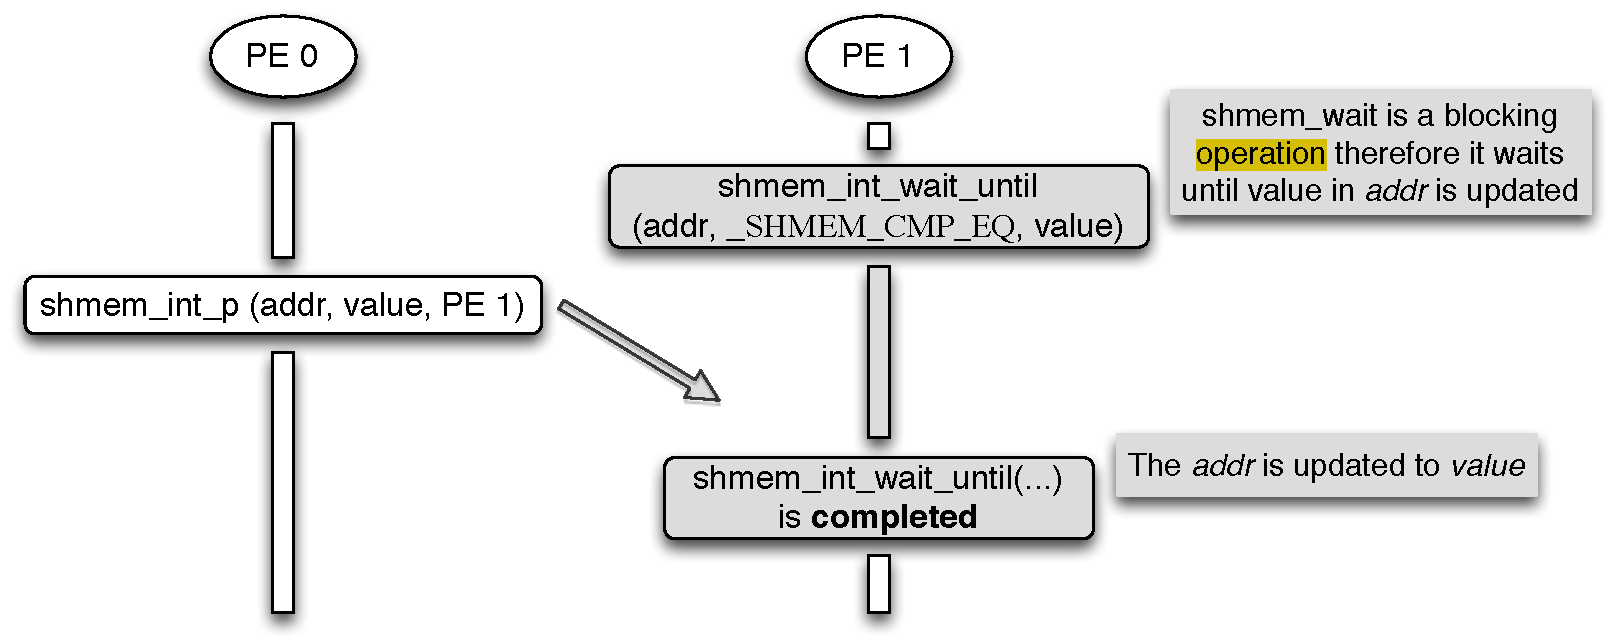
\includegraphics[width=0.7\textwidth]{figures/wait}}
\end{tabular}

\begin{tabular}{p{0.2\textwidth} | p{0.7\textwidth}}
{}
&
Waits for a symmetric variable to be updated by a remote \ac{PE}. Should be
used when computation on the local \ac{PE} cannot proceed without the value that
the remote \ac{PE} is to update. \tabularnewline
\hline 
\end{tabular}

\begin{tabular}{p{0.2\textwidth} | p{0.7\textwidth}}

{Ordering puts issued by a local \ac{PE}} \\
\FUNC{shmem\_fence} 
& 
\raisebox{-\totalheight}{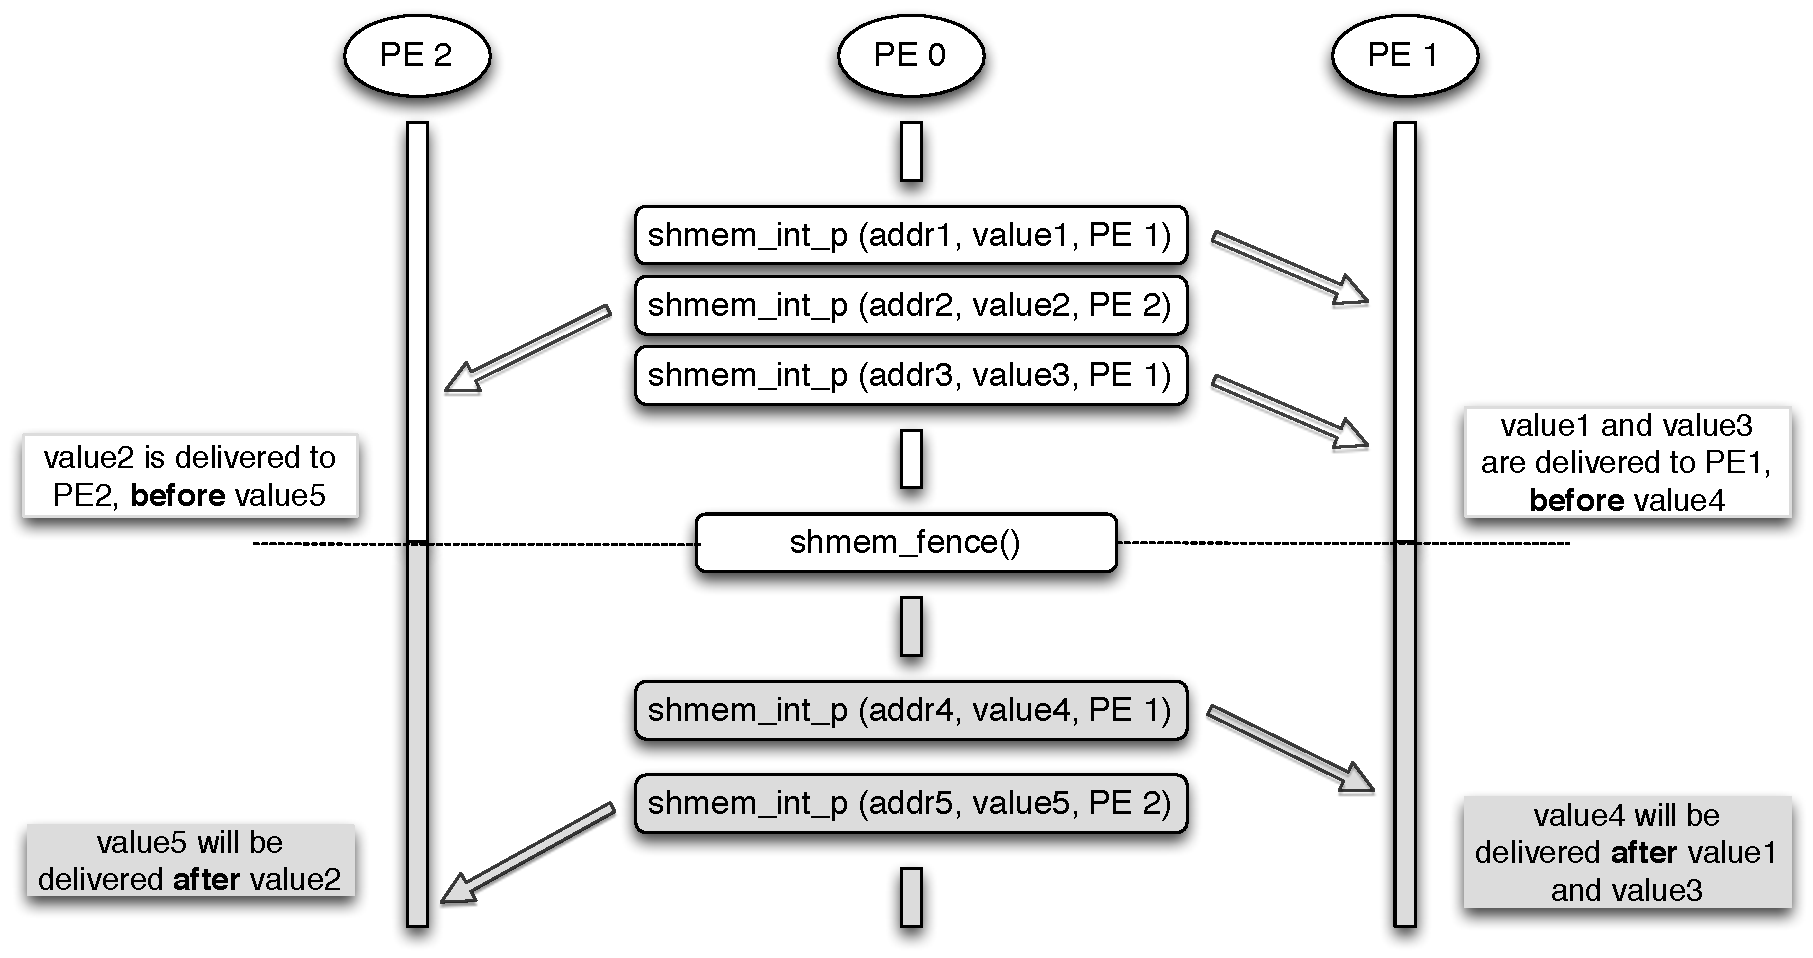
\includegraphics[width=0.7\textwidth]{figures/fence}}
\end{tabular}

\begin{tabular}{p{0.2\textwidth} | p{0.7\textwidth}}
{}
&
All \PUT{}, \ac{AMO}, store, and non-blocking \PUT{} routines on symmetric data issued to
same \ac{PE}  are guaranteed to be delivered  before Puts (to the same \ac{PE})
issued after the \FUNC{fence} call. \tabularnewline
\hline 
\end{tabular}

\begin{tabular}{p{0.2\textwidth} | p{0.7\textwidth}}
\hline 
\textbf{\openshmem  \ac{API}} & \centering \textbf{Working of \openshmem \ac{API}} \tabularnewline
\hline 
\hline
{Ordering puts issued by all \ac{PE} }\\
\FUNC{shmem\_quiet}
& 
\raisebox{-\totalheight}{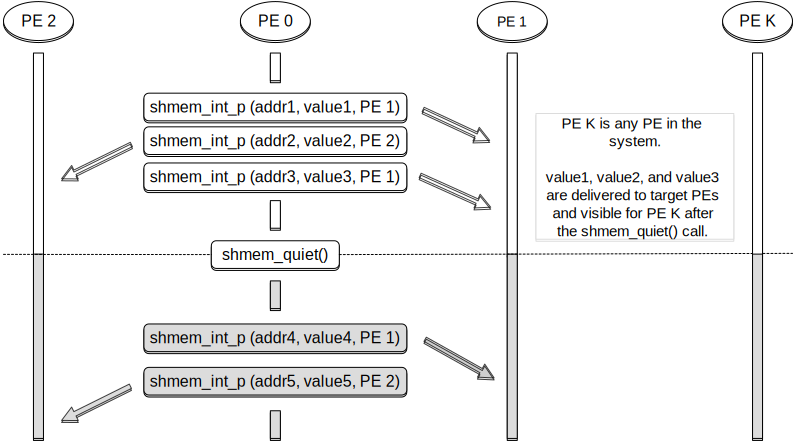
\includegraphics[width=0.7\textwidth]{figures/quiet}} 
\end{tabular}

\begin{tabular}{p{0.2\textwidth} | p{0.7\textwidth}}
{}
&
{All \PUT{}, \ac{AMO}, store, and non-blocking \PUT{} and \GET{} routines on symmetric data issued by a
local \ac{PE} to all  remote \acp{PE} are guaranteed to be completed and visible
once quiet returns. This routine should be used when all remote writes issued by
a local \ac{PE} need to be visible  to all other \acp{PE} before the local
\ac{PE} proceeds. } \tabularnewline
\hline 
\end{tabular}


\begin{tabular}{p{0.2\textwidth} | p{0.7\textwidth}}
Collective synchronization over an active set \\
\FUNC{shmem\_barrier}
&  
\raisebox{-\totalheight}{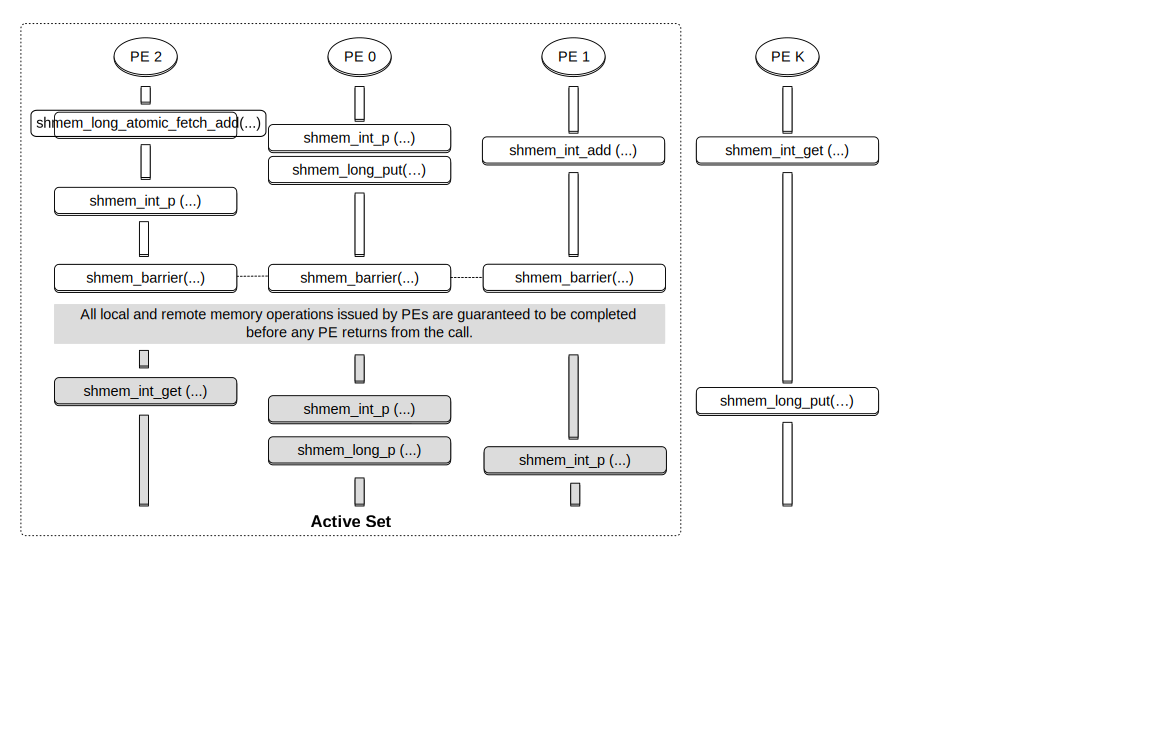
\includegraphics[width=0.7\textwidth]{figures/barrier}} 
\end{tabular}

\begin{tabular}{p{0.2\textwidth} | p{0.7\textwidth}}
{}
&
{All local and remote memory operations issued by all \acp{PE} within the
active set are guaranteed to be completed before any \ac{PE} in the
active set returns from the call. Additionally, no \ac{PE} my return from the
barrier until all \acp{PE} in the active set have entered the same barrier
call. This routine should be used when synchronization as well as completion of
all stores and remote memory updates via \openshmem is required over a sub set
of the executing \acp{PE}.} \tabularnewline
\hline 
\end{tabular}

\begin{tabular}{p{0.2\textwidth} | p{0.7\textwidth}}
\hline 
\textbf{\openshmem  \ac{API}} & \centering \textbf{Working of \openshmem \ac{API}} \tabularnewline
\hline 
\hline
{Collective synchronization over all \acp{PE}} \\
 \FUNC{shmem\_barrier\_all}
& 
\raisebox{-\totalheight}{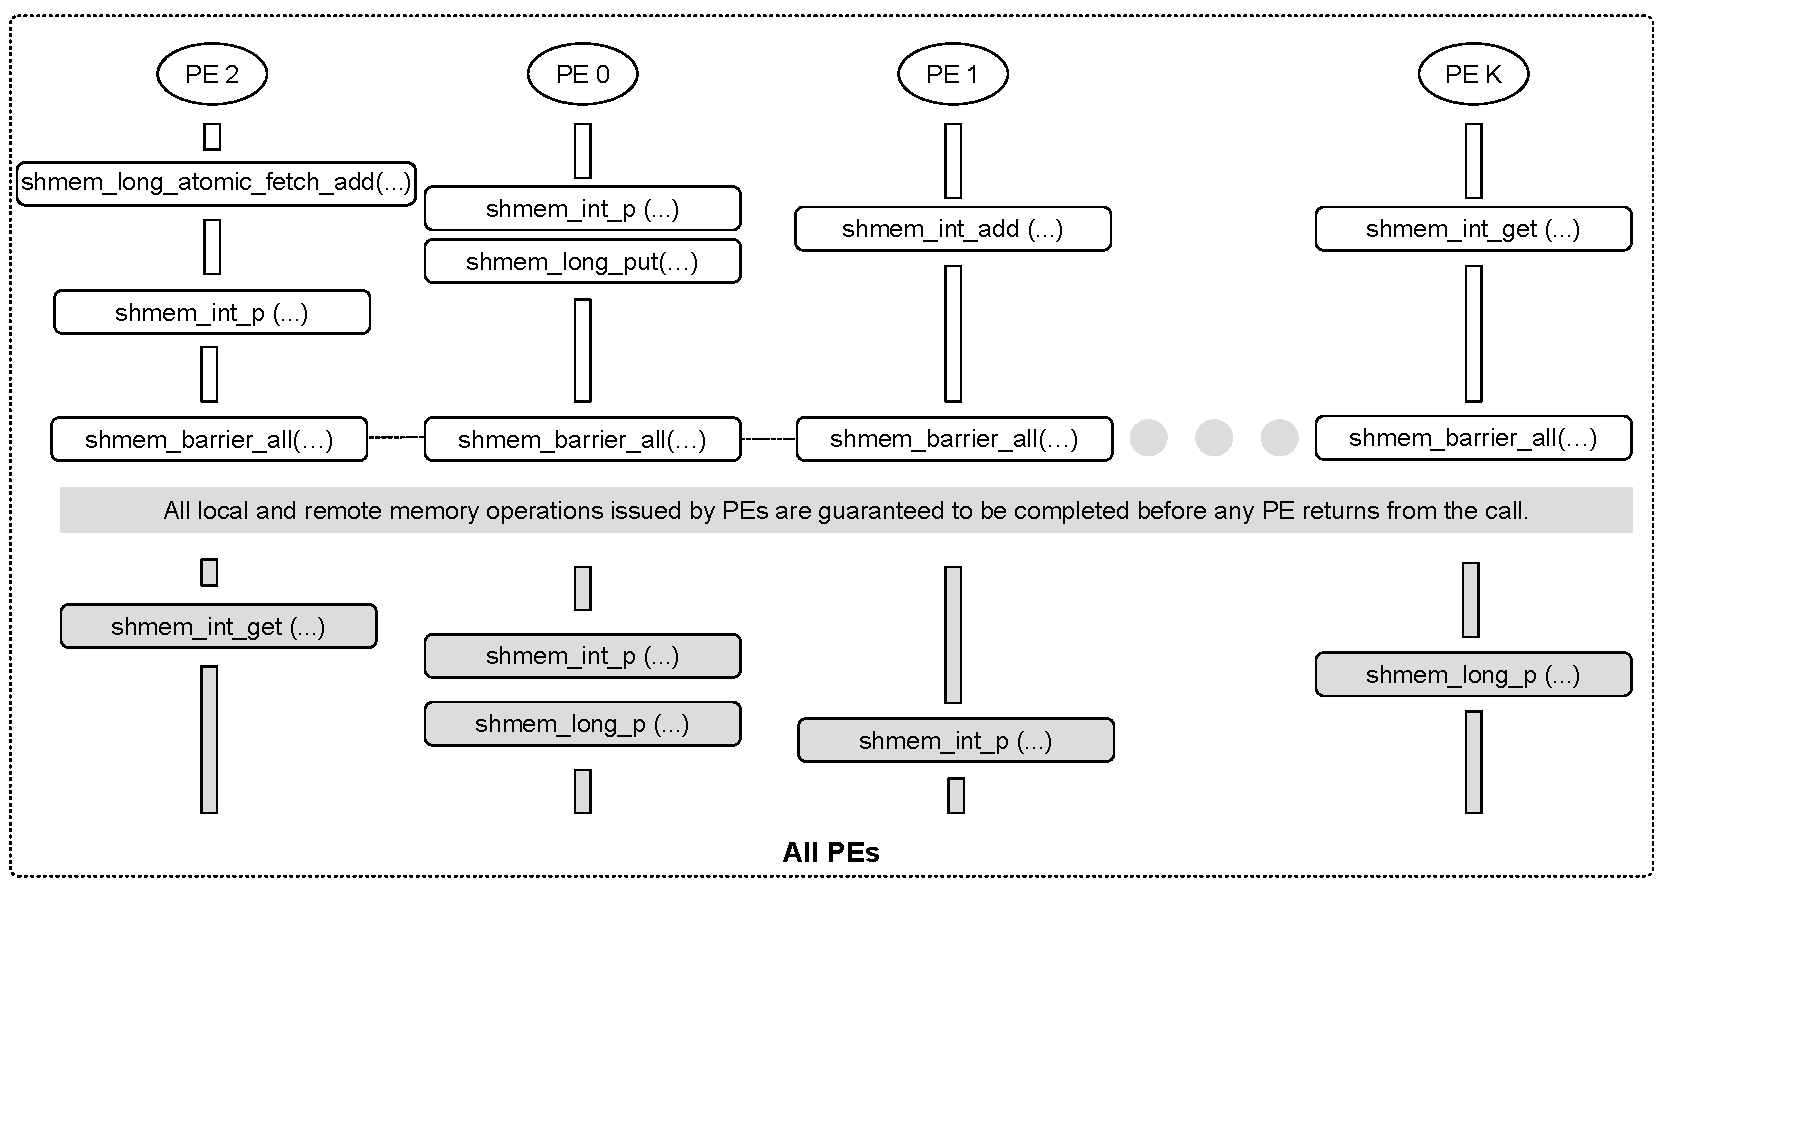
\includegraphics[width=0.7\textwidth]{figures/barrierall}}
\end{tabular}

\begin{tabular}{p{0.2\textwidth} | p{0.7\textwidth}}
{}
&
{All local and remote memory operations issued by all \acp{PE} are guaranteed to
be completed before any \ac{PE} returns from the call. Additionally no \ac{PE}
shall return from the barrier until all \acp{PE} have entered the same
\FUNC{shmem\_barrier\_all} call. This routine should be used when
synchronization as well as completion of all stores and remote memory updates
via \openshmem is required over all \acp{PE}. } \tabularnewline
\hline 
\end{tabular}
\clearpage







\subsection{Distributed Locking Routines}
The following section discusses \openshmem locks as a mechanism to provide
mutual exclusion. Three routines are available for distributed locking,
\textit{set, test} and \textit{clear}.

\subsubsection{\textbf{SHMEM\_LOCK}}\label{subsec:shmem_lock}
\apisummary{
    Releases, locks, and tests a mutual exclusion memory lock.
}
\index{SHMEM\_LOCK}
\begin{apidefinition}

\begin{Csynopsis}
void shmem_clear_lock(long *lock);
void shmem_set_lock(long *lock);
int shmem_test_lock(long *lock);
\end{Csynopsis}

\begin{Fsynopsis}
INTEGER lock, SHMEM_TEST_LOCK
CALL SHMEM_CLEAR_LOCK(lock)
CALL SHMEM_SET_LOCK(lock)
I = SHMEM_TEST_LOCK(lock)
\end{Fsynopsis}

\begin{apiarguments}
\apiargument{IN}{lock}{A symmetric data object that is a scalar variable or an array
    of  length \CONST{1}.  This data  object  must  be set to \CONST{0} on all
    \acp{PE} prior to the first use.  \VAR{lock}  must  be  of type \CONST{long}.
    When using \Fortran, it must be of default kind.}
\end{apiarguments}

\apidescription{
    The \FUNC{shmem\_set\_lock} routine sets a mutual exclusion lock after  waiting
    for  the lock  to be freed by any other \ac{PE} currently holding the lock.
    Waiting \acp{PE} are assured of getting the lock in a first-come, first-served
    manner.  The \FUNC{shmem\_clear\_lock} routine releases a lock  previously set
    by \FUNC{shmem\_set\_lock} after ensuring that all local and remote	 stores
    initiated in the critical region are complete.  The \FUNC{shmem\_test\_lock}
    routine sets a mutual exclusion lock only if it is currently cleared.  By using
    this routine, a \ac{PE} can avoid blocking on a set lock.  If the lock is
    currently set, the routine returns without waiting.  These routines are
    appropriate for protecting a critical region from simultaneous update by
    multiple \acp{PE}.
}

\apireturnvalues{
    The \FUNC{shmem\_test\_lock} routine returns \CONST{0} if  the lock  was
    originally cleared and  this  call was  able  to set the lock.  A value of
    \CONST{1} is returned if the lock had been set and the call returned without
    waiting to set the lock.
}

\apinotes{
    The term symmetric data object is defined in Section \ref{subsec:memory_model}.
    The lock variable should always be initialized to zero and accessed only by the \openshmem locking
    \ac{API}.  Changing the value of the lock variable by other means without using
    the \openshmem \ac{API}, can lead to undefined behavior.
}

\begin{apiexamples}

\apicexample
    {The following example uses \FUNC{shmem\_lock} in a \Cstd[11] program.}
    {./example_code/shmem_lock_example.c}
    {}

\end{apiexamples}

\end{apidefinition}






\section{OpenSHMEM Profiling Interface}\label{sec:openshmem_profiling_interface}
\input{content/profiling_interface.tex}

\clearpage
\clearpage

\appendix

%defining pagestyle for annex
%\pagestyle{plain} \withlinenumbers
\pagestyle{fancy} \withlinenumbers
\fancyhf{}
\fancyhead[RE, LO]{\leftmark}
\fancyhead[RO, LE]{\thepage}
\fancyfoot[CE,CO]{\thepage}
\renewcommand{\headrulewidth}{0pt}




\chapter{Writing OpenSHMEM Programs}
\section*{Incorporating OpenSHMEM into Programs}\label{sec:writing_programs}

The following section describes how to write a ``Hello World" \openshmem program.
To write a ``Hello World" \openshmem program, the user must: 

\begin{itemize}
\item Add the include file \HEADER{shmem.h} for \Cstd or \HEADER{shmem.fh} for \Fortran.
\item Add the initialization call \FUNC{shmem\_init}.
\item Use OpenSHMEM calls to query the total number of \acp{PE} and \ac{PE} id.
\item Add the finalization call \FUNC{shmem\_finalize}.
\item In \openshmem the order in which lines appear in the output is not fixed
    as \acp{PE} execute asynchronously in parallel.
\end{itemize}

\begin{minipage}{\linewidth}
\vspace{0.1in}
\numberedlisting{caption={``Hello World'' example program (C)},label=openshmem-hello,language=OSH2+C}
                {example_code/hello-openshmem.c}
\outputlisting{language=bash,caption={Expected output from the program in Listing~\ref{openshmem-hello} (4 processors)}}
                {example_code/hello-openshmem-c.output}
\vspace{0.1in}
\end{minipage}

\openshmem also has a \Fortran API, therefore listing~\ref{openshmem-hello-f90} provides the same program written in \Fortran:

\begin{minipage}{\linewidth}
\vspace{0.1in}
\numberedlisting{caption={``Hello World'' example program (Fortran)},label=openshmem-hello-f90,language=OSH2+F}
                {example_code/hello-openshmem.f90}
\outputlisting{language=bash,caption={Expected output from the program in Listing~\ref{openshmem-hello-f90} (4 processors)}}
                {example_code/hello-openshmem-f90.output}
\vspace{0.1in}
\end{minipage}

The example in Listing~\ref{openshmem-hello-symmetric} shows a more complex \openshmem program that illustrates
the use of symmetric data objects.  Note the declaration of the  \VAR{static
short dest} array and its use as the remote destination in \openshmem short
\PUT.  The use of the \VAR{static} keyword results in the \VAR{dest} array being
symmetric on \ac{PE} \CONST{0} and \ac{PE} \CONST{1}.  Each \ac{PE} is able to
transfer data to the \dest{} array by simply specifying the local address of the
symmetric data object which is to receive the data.  This aids programmability,
as the address of the \dest{} need not be exchanged with the active side
(\ac{PE} \CONST{0}) prior to the RMA (Remote Memory Access) routine.
Conversely, the declaration of the \VAR{short source} array is asymmetric.
Because the \PUT{} handles the references to the \VAR{source} array only on the
active (local) side, the asymmetric \source{} object is handled correctly.

\begin{minipage}{\linewidth}
\vspace{0.1in}
\numberedlisting{caption={Symmetric data objects example program},label=openshmem-hello-symmetric,language=OSH2+C}
                {example_code/writing_shmem_example.c}
\outputlisting{language=bash,caption={Expected output from the program in Listing~\ref{openshmem-hello-symmetric} (4 processors)}}
                {example_code/writing_shmem_example.output}
\vspace{0.1in}
\end{minipage}




\chapter{Compiling and Running Programs}\label{sec:compiling}
As of this writing, the \openshmem specification is silent regarding how
\openshmem programs are compiled, linked, and run. This section shows some
examples of how wrapper programs are utilized in the \openshmem Reference
Implementation to compile and launch programs.

\section{Compilation}
\subsection*{Programs written in \Cstd}

The \openshmem Reference Implementation provides a wrapper program, named
\textbf{oshcc}, to aid in the compilation of \Cstd programs. The wrapper
could be called as follows:

\begin{lstlisting}[language=bash]
oshcc <compiler options> -o myprogram myprogram.c
\end{lstlisting}
Where the $\langle\mbox{compiler options}\rangle$ are options understood by the
underlying \Cstd compiler.


\subsection*{Programs written in \Cpp}

The  \openshmem Reference Implementation provides a wrapper program, named
\textbf{oshCC}, to aid in the compilation of \Cpp programs. The wrapper could
be called as follows:

\begin{lstlisting}[language=bash]
oshCC <compiler options> -o myprogram myprogram.cpp
\end{lstlisting}
Where the $\langle\mbox{compiler options}\rangle$ are options understood by the
underlying \Cpp compiler called by \textbf{oshCC}.


\subsection*{Programs written in Fortran}

\begin{deprecate}
The \openshmem Reference Implementation provides a wrapper program, named
\textbf{oshfort}, to aid in the compilation of \Fortran programs. The wrapper
could be called as follows:

\begin{lstlisting}[language=bash]
oshfort <compiler options> -o myprogram myprogram.f
\end{lstlisting}
Where the $\langle\mbox{compiler options}\rangle$ are options understood by the
underlying \Fortran compiler called by \textbf{oshfort}.
\end{deprecate}

\section{Running Programs}

The \openshmem Reference Implementation provides a wrapper program, named
\textbf{oshrun}, to launch \openshmem programs. The wrapper could be called as
follows:

\begin{lstlisting}[language=bash]
oshrun <additional options> -np <#> <program> <program arguments>
\end{lstlisting}
The program arguments for \textbf{oshrun} are:

\begin{tabular}{p{0.3\textwidth}p{0.6\textwidth}}
$\langle\mbox{additional options}\rangle$ & {Options passed to the underlying launcher.}\tabularnewline
-np $\langle\mbox{\#}\rangle$ & {The number of \acp{PE} to be used in the execution.}\tabularnewline
$\langle\mbox{program}\rangle$ & {The program executable to be launched.}\tabularnewline
$\langle\mbox{program arguments}\rangle$ & {Flags and other parameters to pass to the program.}\tabularnewline
\end{tabular}





\chapter{Undefined Behavior in OpenSHMEM}\label{sec:undefined}

The specification provides guidelines to the expected behavior of
various library routines.  In cases where routines are improperly used
or the input is not in accordance with the specification, undefined
behavior may be observed.  Depending on the implementation there are
many interpretations of undefined behavior. 

$\;$

$ $%
\begin{tabular}{|>{\raggedright}p{0.3\textwidth}|>{\raggedright}p{0.6\textwidth}|}
\hline 
\textbf{Inappropriate Usage} & \textbf{Undefined Behavior}\tabularnewline
\hline 
\hline 
Uninitialized library & If \openshmem is not initialized through a call to
\FUNC{shmem\_init}, subsequent accesses to \openshmem routines have undefined
results.  An implementation may choose, for example, to try to continue or abort
immediately upon the first call to an uninitialized routine.\tabularnewline
\hline 
Accessing non-existent \acp{PE} & If a communications routine accesses a
non-existent \ac{PE}, then the \openshmem library can choose to handle this
situation in an implementation-defined way.  For example, the library may issue
an error message saying that the \ac{PE} accessed is outside the range of
accessible \acp{PE}, or may exit without a warning.\tabularnewline
\hline 
Use of non-symmetric variables & Some routines require remotely accessible
variables to perform their function.  A \PUT{} to a non-symmetric variable can
be trapped where possible and the library can abort the program.  Another
implementation may choose to continue either with a warning or
silently.\tabularnewline
\hline 
Non-symmetric variables & The symmetric memory management routines are
collectives, which means that all \acp{PE} in the program must issue the same
\FUNC{shmem\_malloc} call with the same size request.  Program behavior after a
mismatched \FUNC{shmem\_malloc} call is undefined.\tabularnewline
\hline 
Use of NULL pointers with non-zero \VAR{len} specified & In any \openshmem routine
that takes a pointer and \VAR{len} describing the number of elements in that
pointer, NULL may not be specified for the pointer unless the corresponding \VAR{len} is also
specified as zero. Otherwise, the resulting behavior is undefined.
The following cases summarize this behavior:
\begin{itemize}
    \item \VAR{len} is 0, pointer is NULL: supported.
    \item \VAR{len} is not 0, pointer is NULL: undefined behavior.
    \item \VAR{len} is 0, pointer is not NULL: supported.
    \item \VAR{len} is not 0, pointer is not NULL: supported.
\end{itemize}
\tabularnewline
\hline 
Multiple calls to \FUNC{shmem\_init} & In an OpenSHMEM program where
\FUNC{shmem\_init} has already be called, any subsequent calls to
\FUNC{shmem\_init} result in undefined behavior.\tabularnewline
\hline 
\end{tabular}







\chapter{Interoperability with other Programming Models}\label{sec:mpi}

\section{\ac{MPI} Interoperability}

\begin{sloppypar} % to prevent constants from running into margins.
%
\openshmem routines can be used in conjunction with \ac{MPI} routines  in the
same program.  For example, on SGI systems, programs that use both \ac{MPI} and
\openshmem routines call \FUNC{MPI\_Init} and \FUNC{MPI\_Finalize} but omit the
call to the \FUNC{shmem\_init} routine.  \openshmem \ac{PE} numbers are equal to
the \ac{MPI} rank within the \CONST{MPI\_COMM\_WORLD} environment variable.
Note that this precludes use of \openshmem routines between processes in
different \CONST{MPI\_COMM\_WORLD}s.  \ac{MPI} processes started using the
\FUNC{MPI\_Comm\_spawn} routine, for example, cannot use \openshmem routines to
communicate with their parent \ac{MPI} processes.
%
\end{sloppypar}
%
On SGI systems where \ac{MPI} jobs use TCP/sockets for inter-host communication,
\openshmem routines can be used to communicate with processes running on the
same host.  The \FUNC{shmem\_pe\_accessible} routine can be used to determine if
a remote \ac{PE} is accessible via \openshmem communication from the local
\ac{PE}. When running an \ac{MPI} program involving multiple executable files,
\openshmem routines can be used to communicate with processes running from the
same or different executable files, provided that the communication is limited
to symmetric data objects.  On these systems, static memory such as a
\Fortran common block or \Cstd global variable, is symmetric between
processes running from the same executable file, but is not symmetric between
processes running from different executable files.  Data allocated from the
symmetric heap (\FUNC{shmem\_malloc} or \FUNC{shpalloc}) is symmetric across the
same or different executable files. The routine \FUNC{shmem\_addr\_accessible}
can be used to determine if a local address is accessible via \openshmem
communication from a remote \ac{PE}.

Another important feature of these systems is that the
\FUNC{shmem\_pe\_accessible} routine returns \CONST{TRUE} only if the remote
\ac{PE} is a process running from the same executable file as the local \ac{PE},
indicating that full \openshmem support (static memory and symmetric heap) is
available.  When using \openshmem routines within an \ac{MPI} program, the use
of \ac{MPI} memory placement environment variables is required when using
non-default memory placement options.

\clearpage







\chapter{History of OpenSHMEM}\label{sec:openshmem_history}

SHMEM has a long history as a parallel programming model, having been used
extensively on a number of products since 1993, including Cray T3D, Cray X1E,
the Cray XT3/4, SGI Origin, SGI Altix, clusters based on the Quadrics
interconnect, and, to a very limited extent, Infiniband based clusters.

\begin{itemize}
\item A SHMEM Timeline
  \begin{itemize}
  \item Cray SHMEM
    \begin{itemize}
    \item SHMEM first introduced by Cray Research Inc. in 1993 for Cray T3D
    \item Cray is acquired by SGI in 1996
    \item Cray is acquired by Tera in 2000 (MTA)
    \item Platforms: Cray T3D, T3E, C90, J90, SV1, SV2, X1, X2, XE, XMT, XT
    \end{itemize}
  \item SGI SHMEM
    \begin{itemize}
    \item SGI purchases  Cray Research Inc. and SHMEM was integrated into
      SGI's Message Passing Toolkit (MPT)
    \item SGI currently owns the rights to SHMEM and \openshmem
    \item Platforms: Origin, Altix 4700, Altix XE, ICE, UV
    \item SGI was purchased by Rackable Systems in 2009
    \item SGI and Open Source Software Solutions, Inc. (OSSS) signed a
      SHMEM trademark licensing agreement, in 2010
    \end{itemize}
  \item Other Implementations
    \begin{itemize}
    \item Quadrics (Vega UK, Ltd.)
    \item Hewlett Packard
    \item GPSHMEM
    \item IBM
    \item QLogic
    \item Mellanox
    % \item University of Houston
    \item University of Florida
    \end{itemize}
  \end{itemize}
\item OpenSHMEM Implementations 
 \begin{itemize}
  \item SGI \openshmem
  \item University of Houston - \openshmem Reference Implementation
  \item Mellanox ScalableSHMEM
  \item Portals-SHMEM
  \item IBM OpenSHMEM
  \end{itemize}
\end{itemize}








\chapter{OpenSHMEM Specification and Deprecated API}\label{sec:dep_api}

\section{Overview}\label{subsec:dep_overview}
For the \openshmem Specification(s), deprecation is the process of identifying
API that is supported but no longer recommended for use by program users. For
\openshmem library users, said API \textbf{must} be supported until clearly
indicated as otherwise by the Specification. This chapter records the
API that has been deprecated, the \openshmem Specification that effected the
deprecation, and if the feature is supported in the current version of the
specification.  

\begin{center}
\scriptsize
\begin{tabular}{|l|c|c|c|}
    \hline
    \textbf{Deprecated API}
    & \textbf{Deprecated Since}
    & \shortstack{\textbf{Last Version Supported}}
    & \textbf{Replaced By} \\
    \hline
    Header Directory: \hyperref[subsec:dep_rationale:mpp]{\HEADER{mpp}} & 1.1 & Current & (none) \\ \hline
    \CorCpp: \hyperref[subsec:start_pes]{\FUNC{start\_pes}} & 1.2 & Current & \hyperref[subsec:shmem_init]{\FUNC{shmem\_init}} \\ \hline
    \Fortran: \hyperref[subsec:start_pes]{\FUNC{START\_PES}} & 1.2 & Current & \hyperref[subsec:shmem_init]{\FUNC{SHMEM\_INIT}} \\ \hline
    \hyperref[subsec:start_pes]{Implicit finalization} & 1.2 & Current & \hyperref[subsec:shmem_finalize]{\FUNC{shmem\_finalize}} \\ \hline
    \CorCpp: \FUNC{\_my\_pe} & 1.2 & Current & \hyperref[subsec:shmem_my_pe]{\FUNC{shmem\_my\_pe}} \\ \hline
    \CorCpp: \FUNC{\_num\_pes} & 1.2 & Current & \hyperref[subsec:shmem_n_pes]{\FUNC{shmem\_n\_pes}} \\ \hline
    \Fortran: \FUNC{MY\_PE} & 1.2 & Current & \hyperref[subsec:shmem_my_pe]{\FUNC{SHMEM\_MY\_PE}} \\ \hline
    \Fortran: \FUNC{NUM\_PES} & 1.2 & Current & \hyperref[subsec:shmem_n_pes]{\FUNC{SHMEM\_N\_PES}} \\ \hline
    \CorCpp: \FUNC{shmalloc} & 1.2 & Current & \hyperref[subsec:shfree]{\FUNC{shmem\_malloc}} \\ \hline
    \CorCpp: \FUNC{shfree} & 1.2 & Current & \hyperref[subsec:shfree]{\FUNC{shmem\_free}} \\ \hline
    \CorCpp: \FUNC{shrealloc} & 1.2 & Current & \hyperref[subsec:shfree]{\FUNC{shmem\_realloc}} \\ \hline
    \CorCpp: \FUNC{shmemalign} & 1.2 & Current & \hyperref[subsec:shfree]{\FUNC{shmem\_align}} \\ \hline
    \Fortran: \FUNC{SHMEM\_PUT} & 1.2 & Current & \hyperref[subsec:shmem_put]{\FUNC{SHMEM\_PUT8} or \FUNC{SHMEM\_PUT64}} \\ \hline
    \shortstack[l]{\CorCpp: \hyperref[subsec:shmem_cache]{\FUNC{shmem\_clear\_cache\_inv}}
        \\ \Fortran: \hyperref[subsec:shmem_cache]{\FUNC{SHMEM\_CLEAR\_CACHE\_INV}}}
        & 1.3 & Current & (none) \\ \hline
    \CorCpp: \hyperref[subsec:shmem_cache]{\FUNC{shmem\_clear\_cache\_line\_inv}} & 1.3 & Current & (none) \\ \hline
    \shortstack[l]{\CorCpp: \hyperref[subsec:shmem_cache]{\FUNC{shmem\_set\_cache\_inv}}
        \\ \Fortran: \hyperref[subsec:shmem_cache]{\FUNC{SHMEM\_SET\_CACHE\_INV}}}
        & 1.3 & Current & (none) \\ \hline
    \shortstack[l]{\CorCpp: \hyperref[subsec:shmem_cache]{\FUNC{shmem\_set\_cache\_line\_inv}}
        \\ \Fortran: \hyperref[subsec:shmem_cache]{\FUNC{SHMEM\_SET\_CACHE\_LINE\_INV}}}
        & 1.3 & Current & (none) \\ \hline
    \shortstack[l]{\CorCpp: \hyperref[subsec:shmem_cache]{\FUNC{shmem\_udcflush}}
        \\ \Fortran: \hyperref[subsec:shmem_cache]{\FUNC{SHMEM\_UDCFLUSH}}}
        & 1.3 & Current & (none) \\ \hline
    \shortstack[l]{\CorCpp: \hyperref[subsec:shmem_cache]{\FUNC{shmem\_udcflush\_line}}
        \\ \Fortran: \hyperref[subsec:shmem_cache]{\FUNC{SHMEM\_UDCFLUSH\_LINE}}}
        & 1.3 & Current & (none) \\ \hline
    \_SHMEM\_SYNC\_VALUE & 1.3 & Current & \hyperref[subsec:library_constants]{SHMEM\_SYNC\_VALUE} \\ \hline
    \_SHMEM\_BARRIER\_SYNC\_SIZE & 1.3 & Current & \hyperref[subsec:library_constants]{SHMEM\_BARRIER\_SYNC\_SIZE} \\ \hline
    \_SHMEM\_BCAST\_SYNC\_SIZE & 1.3 & Current & \hyperref[subsec:library_constants]{SHMEM\_BCAST\_SYNC\_SIZE} \\ \hline
    \_SHMEM\_COLLECT\_SYNC\_SIZE & 1.3 & Current & \hyperref[subsec:library_constants]{SHMEM\_COLLECT\_SYNC\_SIZE} \\ \hline
    \_SHMEM\_REDUCE\_SYNC\_SIZE & 1.3 & Current & \hyperref[subsec:library_constants]{SHMEM\_REDUCE\_SYNC\_SIZE} \\ \hline
    \_SHMEM\_REDUCE\_MIN\_WRKDATA\_SIZE & 1.3 & Current & \hyperref[subsec:library_constants]{SHMEM\_REDUCE\_MIN\_WRKDATA\_SIZE} \\ \hline
    \_SHMEM\_MAJOR\_VERSION & 1.3 & Current & \hyperref[subsec:library_constants]{SHMEM\_MAJOR\_VERSION} \\ \hline
    \_SHMEM\_MINOR\_VERSION & 1.3 & Current & \hyperref[subsec:library_constants]{SHMEM\_MINOR\_VERSION} \\ \hline
    \_SHMEM\_MAX\_NAME\_LEN & 1.3 & Current & \hyperref[subsec:library_constants]{SHMEM\_MAX\_NAME\_LEN} \\ \hline
    \_SHMEM\_VENDOR\_STRING & 1.3 & Current & \hyperref[subsec:library_constants]{SHMEM\_VENDOR\_STRING} \\ \hline
    SMA\_VERSION         & 1.4 & Current & \hyperref[subsec:environment_variables]{SHMEM\_VERSION} \\ \hline
    SMA\_INFO            & 1.4 & Current & \hyperref[subsec:environment_variables]{SHMEM\_INFO} \\ \hline
    SMA\_SYMMETRIC\_SIZE & 1.4 & Current & \hyperref[subsec:environment_variables]{SHMEM\_SYMMETRIC\_SIZE} \\ \hline
    SMA\_DEBUG           & 1.4 & Current & \hyperref[subsec:environment_variables]{SHMEM\_DEBUG} \\ \hline
    \CorCpp: \FUNC{shmem\_wait}  & 1.4 & Current & See ``Notes'' for \hyperref[subsec:shmem_wait]{\FUNC{shmem\_wait\_until}} \\ \hline
    \CorCpp: \FUNC{shmem\_fetch} & 1.4 & Current & \hyperref[subsec:shmem_atomic_fetch]{\FUNC{shmem\_atomic\_fetch}} \\ \hline
    \CorCpp: \FUNC{shmem\_set}   & 1.4 & Current & \hyperref[subsec:shmem_atomic_set]{\FUNC{shmem\_atomic\_set}} \\ \hline
    \CorCpp: \FUNC{shmem\_cswap} & 1.4 & Current & \hyperref[subsec:shmem_atomic_compare_swap]{\FUNC{shmem\_atomic\_compare\_swap}} \\ \hline
    \CorCpp: \FUNC{shmem\_swap}  & 1.4 & Current & \hyperref[subsec:shmem_atomic_swap]{\FUNC{shmem\_atomic\_swap}} \\ \hline
    \CorCpp: \FUNC{shmem\_finc}  & 1.4 & Current & \hyperref[subsec:shmem_atomic_fetch_inc]{\FUNC{shmem\_atomic\_fetch\_inc}} \\ \hline
    \CorCpp: \FUNC{shmem\_inc}   & 1.4 & Current & \hyperref[subsec:shmem_atomic_inc]{\FUNC{shmem\_atomic\_inc}} \\ \hline
    \CorCpp: \FUNC{shmem\_fadd}  & 1.4 & Current & \hyperref[subsec:shmem_atomic_fetch_add]{\FUNC{shmem\_atomic\_fetch\_add}} \\ \hline
    \CorCpp: \FUNC{shmem\_add}   & 1.4 & Current & \hyperref[subsec:shmem_atomic_add]{\FUNC{shmem\_atomic\_add}} \\ \hline
    Entire \Fortran API & 1.4 & Current & (none) \\ \hline
    \end{tabular}
\end{center}

\section{Deprecation Rationale}\label{subsec:dep_rationale}

\subsection{Header Directory: \HEADER{mpp}}
\label{subsec:dep_rationale:mpp}
In addition to the default system header paths, \openshmem implementations
must provide all \openshmem standard header files from the \HEADER{mpp}
header directory such that headers can be referenced in \CorCpp as
\begin{lstlisting}[language=]
#include <mpp/shmem.h>
#include <mpp/shmemx.h>
\end{lstlisting}
and in \Fortran as
\begin{lstlisting}[language=]
include 'mpp/shmem.fh'
include 'mpp/shmemx.fh'
\end{lstlisting}
for backwards compatibility with SGI SHMEM.

\subsection{\CorCpp: start\_pes}
The \CorCpp routine \FUNC{start\_pes} includes an unnecessary initialization
argument that is remnant of historical \emph{SHMEM} implementations and no
longer reflects the requirements of modern \openshmem implementations.
Furthermore, the naming of \FUNC{start\_pes} does not include the standardized
\shmemprefixLC{} naming prefix. This routine has been deprecated and
\openshmem users are encouraged to use
\hyperref[subsec:shmem_init]{\FUNC{shmem\_init}} instead.

\subsection{\CorCpp: \_my\_pe, \_num\_pes, shmalloc, shfree, shrealloc, shmemalign}
The \CorCpp routines \FUNC{\_my\_pe}, \FUNC{\_num\_pes}, \FUNC{shmalloc},
\FUNC{shfree}, \FUNC{shrealloc}, and \FUNC{shmemalign} were deprecated in order
to normalize the \openshmem \ac{API} to use \shmemprefixLC{} as the standard
prefix for all routines.

\subsection{Implicit Finalization}
Implicit finalization has been replaced with explicit finalization using the
\FUNC{shmem\_finalize} routine.  Explicit finalization improves portability and
also improves interoperability with profiling and debugging tools.

\subsection{Fortran: START\_PES, MY\_PE, NUM\_PES}
The \Fortran routines \FUNC{START\_PES}, \FUNC{MY\_PE}, and \FUNC{NUM\_PES}
were deprecated in order to minimize the API differences from the deprecation
of \CorCpp routines \FUNC{start\_pes}, \FUNC{\_my\_pe}, and \FUNC{\_num\_pes}.

\subsection{Fortran: SHMEM\_PUT}
The \Fortran function \FUNC{SHMEM\_PUT} is defined only for the \Fortran
\ac{API} and is semantically identical to \Fortran functions
\FUNC{SHMEM\_PUT8} and \FUNC{SHMEM\_PUT64}.  Since \FUNC{SHMEM\_PUT8} and
\FUNC{SHMEM\_PUT64} have defined equivalents in the \CorCpp interface,
\FUNC{SHMEM\_PUT} is ambiguous and has been deprecated.

\subsection{SHMEM\_CACHE}
The \FUNC{SHMEM\_CACHE} \ac{API}
\begin{center}
\begin{tabular}{ll}
    \CorCpp: & \Fortran: \\
    shmem\_clear\_cache\_inv & SHMEM\_CLEAR\_CACHE\_INV \\
    shmem\_set\_cache\_inv & SHMEM\_SET\_CACHE\_INV \\
    shmem\_set\_cache\_line\_inv & SHMEM\_SET\_CACHE\_LINE\_INV \\
    shmem\_udcflush & SHMEM\_UDCFLUSH \\
    shmem\_udcflush\_line & SHMEM\_UDCFLUSH\_LINE \\
    shmem\_clear\_cache\_line\_inv \\
\end{tabular}
\end{center}
was originally implemented for systems with cache management instructions.
This API has largely gone unused on cache-coherent system architectures.
\FUNC{SHMEM\_CACHE} has been deprecated.

\subsection{\_SHMEM\_* Library Constants}
The library constants
\begin{center}
\begin{tabular}{ll}
    \_SHMEM\_SYNC\_VALUE & \_SHMEM\_REDUCE\_MIN\_WRKDATA\_SIZE \\
    \_SHMEM\_BARRIER\_SYNC\_SIZE & \_SHMEM\_MAJOR\_VERSION \\
    \_SHMEM\_BCAST\_SYNC\_SIZE & \_SHMEM\_MINOR\_VERSION \\
    \_SHMEM\_COLLECT\_SYNC\_SIZE & \_SHMEM\_MAX\_NAME\_LEN \\
    \_SHMEM\_REDUCE\_SYNC\_SIZE & \_SHMEM\_VENDOR\_STRING \\
\end{tabular}
\end{center}
do not adhere to the \Cstd standard's reserved identifiers and the \Cpp
standard's reserved names.  These constants have been deprecated and replaced
with corresponding constants of prefix \shmemprefix{} that adhere to \CorCpp{}
and \Fortran naming conventions.

\subsection{\FUNC{shmem\_fetch}, \FUNC{shmem\_set}, \FUNC{shmem\_cswap},
  \FUNC{shmem\_swap}, \FUNC{shmem\_finc}, \FUNC{shmem\_inc},
  \FUNC{shmem\_fadd}, \FUNC{shmem\_add}}

The \CorCpp interfaces for \FUNC{shmem\_fetch}, \FUNC{shmem\_set},
\FUNC{shmem\_cswap}, \FUNC{shmem\_swap}, \FUNC{shmem\_finc}, \FUNC{shmem\_inc},
\FUNC{shmem\_fadd}, and \FUNC{shmem\_add} were deprecated and replaced with
similarly-named interfaces within the \FUNC{shmem\_atomic\_*} namespace
in order to more clearly identify these calls as performing atomic operations.
In addition, the abbreviated names ``cswap'', ``finc'', and ``fadd'' were
expanded for clarity to ``compare\_swap'', ``fetch\_inc'', and ``fetch\_add''.

\subsection{SMA\_* Environment Variables}
The environment variables
\begin{center}
\begin{tabular}{ll}
    SMA\_VERSION \\
    SMA\_INFO \\
    SMA\_SYMMETRIC\_SIZE \\
    SMA\_DEBUG \\
\end{tabular}
\end{center}
were deprecated in order to normalize the \openshmem \ac{API} to use
\shmemprefix{} as the standard prefix for all environment variables.

\subsection{Fortran API}\label{subsec:deprecate-fortran}
The entire \openshmem \Fortran API was deprecated because of a general lack of
use and a lack of conformance with legacy \Fortran standards. In lieu of an
extensive update of the \Fortran API, \Fortran users are encouraged to
leverage current and future \openshmem specifications of the \Cstd API
through the \Fortran-\Cstd interoperability initially standardized by
\Fortran[2003]%
\footnote{Formally, \Fortran[2003] is known as ISO/IEC~1539-1:2004(E).}.

\subsection{\FUNC{shmem\_wait}}
The \FUNC{shmem\_wait} interface was identified as unintuitive with respect to
the comparison operation it performed.  As \FUNC{shmem\_wait} can be trivially
replaced by \FUNC{shmem\_wait\_until} where \VAR{cmp} is
\CONST{SHMEM\_CMP\_NE}, the \FUNC{shmem\_wait} interface was deprecated in
favor of \FUNC{shmem\_wait\_until}, which makes the comparison operation
explicit and better communicates the developer's intent.





\chapter{Changes to this Document}\label{sec:changelog}

\section{Version 1.4}

\begin{itemize}

\item Clarified that the \openshmem extensions header files are required, even when empty.
\\See Section~\ref{subsec:bindings}.
%
\item Clarified that the \FUNC{SHMEM\_GET64} and \FUNC{SHMEM\_GET64\_NBI}
    routines are included in the Fortran language bindings.\\
    See Sections \ref{subsec:shmem_get} and \ref{subsec:shmem_get_nbi}.
%
\item Clarified that \FUNC{shmem\_init} must be matched with a call to
    \FUNC{shmem\_finalize}.
\\See Sections \ref{subsec:shmem_init} and \ref{subsec:shmem_finalize}.
%
\item Added the \VAR{SHMEM\_SYNC\_SIZE} constant.
\\See Section \ref{subsec:library_constants}.
%
\item Added type-generic interfaces for \FUNC{SHMEM\_WAIT}.
\\ See Section \ref{subsec:shmem_wait}.
%
\item Removed the \VAR{volatile} qualifiers from the \VAR{ivar} arguments to
\FUNC{shmem\_wait} routines and the \VAR{lock} arguments in the lock API.
\emph{Rationale: Volatile qualifiers were added to several API routines in
version 1.3 of the OpenSHMEM specification; however, they were later found
to be unnecessary.}
\\ See Sections \ref{subsec:shmem_wait} and \ref{subsec:shmem_lock}.
%
\item Deprecated the \VAR{SMA\_}* environment variables and added equivalent
\VAR{SHMEM\_}* environment variables.
\\ See Section \ref{subsec:environment_variables}.
%
\item Added the \Cstd[11] \CTYPE{\_Noreturn} function specifier to
\FUNC{shmem\_global\_exit}.
\\ See Section \ref{subsec:shmem_global_exit}.
%
\item Clarified ordering semantics of memory ordering, point-to-point synchronization, and collective 
synchronization routines.
%
\item Clarified deprecation overview and added deprecation rationale in Annex F.
\\See Section \ref{sec:dep_api}.
%
\item Deprecated header directory \HEADER{mpp}.
\\See Section \ref{sec:dep_api}.
%
\item Deprecated the \VAR{shmem\_wait} functions and added \VAR{shmem\_test}
      functions.
\\ See Section \ref{subsec:p2p_intro}.
%
\item Added the \FUNC{shmem\_calloc} function.
\\ See Section \ref{subsec:shmem_calloc}.
%
\item Introduced the thread safe semantics that define the interaction between
    \openshmem routines and user threads.
\\See Section \ref{subsec:thread_support}.
%
\item Added the new routine \FUNC{shmem\_init\_thread} to initialize the
    \openshmem library with one of the defined thread levels.
\\See Section \ref{subsec:shmem_init_thread}.
%
\item Added the new routine \FUNC{shmem\_query\_thread} to query the thread
    level provided by the \openshmem implementation.
\\See Section \ref{subsec:shmem_query_thread}.
%
\item Clarified the semantics of \FUNC{shmem\_quiet} for a multithreaded
    \openshmem \ac{PE}.
\\See Section \ref{subsec:shmem_quiet}
%
\item Revised the description of \FUNC{shmem\_barrier\_all} for a multithreaded
    \openshmem \ac{PE}.
\\See Section \ref{subsec:shmem_barrier_all}
%
\item Revised the description of \FUNC{shmem\_wait} for a multithreaded
    \openshmem \ac{PE}.
\\See Section \ref{subsec:shmem_wait}
%
\item Clarified description for \CONST{SHMEM\_VENDOR\_STRING}.
\\See Section \ref{subsec:library_constants}.
%
\item Clarified description for \CONST{SHMEM\_MAX\_NAME\_LEN}.
\\See Section \ref{subsec:library_constants}.
%
\item Clarified API description for \FUNC{shmem\_info\_get\_name}.
\\See Section \ref{subsec:shmem_info_get_name}.
%
\item Expanded the type support for RMA and AMO operations.
\\ See Sections \ref{sec:rma} and \ref{sec:amo}.
%
\item Renamed AMO operations to use \FUNC{shmem\_atomic\_*} prefix and
      deprecated old AMO routines.
\\ See Section \ref{sec:amo}.
%
\item Added fetching and non-fetching bitwise AND, OR, and XOR atomic
      operations.
\\ See Section \ref{sec:amo}.
%
\item Deprecated the entire \Fortran API.
%
\item Replaced the \CTYPE{complex} macro in complex-typed reductions with the
      \Cstd[99] (and later) type specifier \CTYPE{\_Complex} to remove an
      implicit dependence on \HEADER{complex.h}.
\\ See Section \ref{subsec:shmem_reductions}.
%
\item Clarified that complex-typed reductions in C are optionally supported.
\\ See Section \ref{subsec:shmem_reductions}.
%
\end{itemize}

\section{Version 1.3}
This section summarizes the changes from the \openshmem specification Version
1.2 to Version 1.3. Many major changes to the specification were introduced in Version 1.3. This includes non-blocking RMA operations, 
generic interfaces for various OpenSHMEM interfaces, atomic \FUNC{Put} and \FUNC{Get} operations,  and Alltoall interfaces. 


The following list describes the specific changes in 1.3:

\begin{itemize}
%
\item Clarified implementation of \acp{PE} as threads.
%
\item Added \CTYPE{const} to every read-only pointer argument.
%
\item Clarified definition of \OPR{Fence}.
\\See Section \ref{subsec:programming_model}.
%
\item Clarified implementation of symmetric memory allocation.
\\See Section \ref{subsec:memory_model}.
%
\item Restricted atomic operation guarantees to other atomic operations with the same datatype.
\\See Section \ref{subsec:amo_guarantees}.
%
\item Deprecation of all constants that start with \CONST{\_SHMEM\_*}.
\\See Section \ref{subsec:library_constants}.
%
\item Added a type-generic interface to \openshmem \ac{RMA} and \ac{AMO}
	operations based on \Cstd[11] Generics.
\\See Sections \ref{sec:rma}, \ref{sec:rma_nbi} and \ref{sec:amo}.
%
\item New non-blocking variants of remote memory access, \FUNC{SHMEM\_PUT\_NBI}
	and \FUNC{SHMEM\_GET\_NBI}.
\\See Sections \ref{subsec:shmem_put_nbi} and \ref{subsec:shmem_get_nbi}.
%
\item New atomic elemental read and write operations, \FUNC{SHMEM\_FETCH} and
	\FUNC{SHMEM\_SET}.
\\See Sections \ref{subsec:shmem_atomic_fetch} and \ref{subsec:shmem_atomic_set}
%
\item New alltoall data exchange operations, \FUNC{SHMEM\_ALLTOALL} 
	and \FUNC{SHMEM\_ALLTOALLS}.
\\See Sections \ref{subsec:shmem_alltoall} and \ref{subsec:shmem_alltoalls}.
%
\item Added \CTYPE{volatile} to remotely accessible pointer argument in
	\FUNC{SHMEM\_WAIT} and \FUNC{SHMEM\_LOCK}.
\\See Sections \ref{subsec:shmem_wait} and \ref{subsec:shmem_lock}.
%
\item Deprecation of \FUNC{SHMEM\_CACHE}.
\\See Section \ref{subsec:shmem_cache}.
%
\end{itemize}




\section{Version 1.2}
This section summarizes the changes from the \openshmem specification Version
1.1 to Version 1.2.  A major change in this version is that it improves upon the
execution model described in 1.1 by introducing an explicit
\FUNC{shmem\_finalize} library call. This provides a collective mechanism of
exiting an \openshmem program and releasing resources used by the library.  


The following list describes the specific changes in 1.2:

\begin{itemize}
%
\item Added specification of \VAR{pSync} initialization for all routines that use it.
%
\item Replaced all placeholder variable names \VAR{target} with \VAR{dest} to
      avoid confusion with Fortran `target' keyword.
%
\item New Execution Model for exiting/finishing OpenSHMEM programs.
\\See Section  \ref{subsec:execution_model}.
%
\item New library constants to support API that query version and name information.
\\See Section \ref{subsec:library_constants}.
%
\item New API \FUNC{shmem\_init} to provide mechanism to start an \openshmem
      program and replace deprecated \FUNC{start\_pes}.
\\See Section \ref{subsec:shmem_init}.
%
\item Deprecation of \FUNC{\_my\_pe} and \FUNC{\_num\_pes} routines.
\\See Sections \ref{subsec:shmem_my_pe} and \ref{subsec:shmem_n_pes}.
%
\item New API \FUNC{shmem\_finalize} to provide collective mechanism to cleanly
      exit an \openshmem program and release resources.
\\See Section \ref{subsec:shmem_finalize}.
%
\item New API \FUNC{shmem\_global\_exit} to provide mechanism to exit an
    \openshmem program.
\\See Section \ref{subsec:shmem_global_exit}.
%
\item Clarification related to the address of the referenced object in
    \FUNC{shmem\_ptr}.
\\See Section \ref{subsec:shmem_ptr}.
%
\item New API to query the version and name information. 
\\See Section \ref{subsec:shmem_info_get_version} and \ref{subsec:shmem_info_get_name}.
%
\item \openshmem library API normalization. All \Cstd symmetric memory management
      API begins with  \FUNC{shmem\_}.
\\See Section \ref{subsec:shfree}.
%
\item Notes and clarifications added to \FUNC{shmem\_malloc}.
\\See Section \ref{subsec:shfree}.
%
\item Deprecation of Fortran API routine \FUNC{SHMEM\_PUT}.
\\See Section \ref{subsec:shmem_put}. 
%
\item Clarification related to \FUNC{shmem\_wait}.
\\See Section \ref{subsec:shmem_wait}.
%
\item Undefined behavior for null pointers without zero counts added.
\\See Annex \ref{sec:undefined}
%
\item Addition of new Annex for clearly specifying deprecated API and its
      support in the existing specification version.
\\See Annex \ref{sec:dep_api}.
%
\end{itemize}




\section{Version 1.1}
This section summarizes the changes from the \openshmem specification Version
1.0 to the Version 1.1.  A major change in this version is that it provides an
accurate description of \openshmem interfaces so that they are in agreement with
the SGI specification.  This version also explains \openshmem's programming,
memory, and execution model.  The document was thoroughly changed to improve the
readability of specification and usability of interfaces.  The code examples
were added to demonstrate the usability of API. Additionally, diagrams were
added to help understand the subtle semantic differences of various operations.


The following list describes the specific changes in 1.1:

\begin{itemize}
%
\item Clarifications of the completion semantics of memory synchronization 
      interfaces.
\\See Section \ref{subsec:memory_order}.
%
\item Clarification of the completion semantics of memory load and store
      operations in context of \FUNC{shmem\_barrier\_all} and \FUNC{shmem\_barrier}
      routines.
\\See Section \ref{subsec:shmem_barrier_all} and \ref{subsec:shmem_barrier}.
%
\item Clarification of the completion and ordering semantics of
      \FUNC{shmem\_quiet} and \FUNC{shmem\_fence}.
\\See Section \ref{subsec:shmem_quiet} and \ref{subsec:shmem_fence}.
%
\item Clarifications of the completion semantics of \ac{RMA} and \ac{AMO}
      routines.
\\See Sections \ref{sec:rma} and \ref{sec:amo}
%
\item Clarifications of the memory model and the memory alignment requirements
      for symmetric data objects.
\\See Section \ref{subsec:memory_model}.
%
\item Clarification of the execution model and the definition of a \ac{PE}.
\\See Section \ref{subsec:execution_model}
%
\item Clarifications of the semantics of \FUNC{shmem\_pe\_accessible} and
      \FUNC{shmem\_addr\_accessible}.
\\See Section \ref{subsec:shmem_pe_accessible} and \ref{subsec:shmem_addr_accessible}.
%
\item Added an annex on interoperability with \ac{MPI}.
\\See Annex \ref{sec:mpi}.
%
\item Added examples to the different interfaces.
%
\item Clarification of the naming conventions for constant in \Cstd and
      \Fortran.
\\See Section \ref{subsec:library_constants} and \ref{subsec:shmem_wait}.
%
\item Added \ac{API} calls: \FUNC{shmem\_char\_p}, \FUNC{shmem\_char\_g}.
\\See Sections \ref{subsec:shmem_p} and \ref{subsec:shmem_g}. 
%
\item Removed \ac{API} calls: \FUNC{shmem\_char\_put},
      \FUNC{shmem\_char\_get}.
\\See Sections \ref{subsec:shmem_put} and \ref{subsec:shmem_get}. 
%
\item The usage of \VAR{ptrdiff\_t}, \VAR{size\_t}, and \VAR{int} in the
      interface signature was made consistent with the description.
\\See Sections \ref{subsec:coll}, \ref{subsec:shmem_iput}, and \ref{subsec:shmem_iget}.
%
\item Revised \FUNC{shmem\_barrier} example.
\\See Section \ref{subsec:shmem_barrier}. 
%
\item Clarification of the initial value of \VAR{pSync} work arrays for
\FUNC{shmem\_barrier}.\\ See Section \ref{subsec:shmem_barrier}. 
%
\item Clarification of the expected behavior when multiple \FUNC{start\_pes}
calls are encountered has been clarified.
\\See Section \ref{subsec:start_pes}.
%
\item Corrected the definition of atomic increment operation.
\\See Section \ref{subsec:shmem_atomic_inc}.
%
\item Clarification of the size of the symmetric heap and when it is set.
\\See Section \ref{subsec:shfree}.
%
\item Clarification of the integer and real sizes for \Fortran \ac{API}.
\\See Sections \ref{subsec:shmem_atomic_add},
      \ref{subsec:shmem_atomic_compare_swap},
      \ref{subsec:shmem_atomic_swap},
      \ref{subsec:shmem_atomic_fetch_inc},
      \ref{subsec:shmem_atomic_inc}, and
      \ref{subsec:shmem_atomic_fetch_add}.
%
\item Clarification of the expected behavior on program \OPR{exit}.
\\See Section \ref{subsec:execution_model}, Execution Model. 
%
\item More detailed description for the progress of \openshmem operations
provided.
\\See Section \ref{subsec:progress}. 
%
\item Clarification of naming convention for non-standard interfaces and their
inclusion in \HEADER{shmemx.h}.
\\See Section \ref{subsec:bindings}. 
%
\item Various fixes to \openshmem code examples across the specification to
include appropriate header files. 
%
\item Removing requirement that implementations should detect size mismatch and
return error information for \FUNC{shmalloc} and ensuring consistent
language.
\\See Sections \ref{subsec:shfree} and Annex \ref{sec:undefined}. 
%
\item Fortran programming fixes for examples.\\ See Sections
\ref{subsec:shmem_reductions} and \ref{subsec:shmem_wait}. 
%
\item Clarifications of the reuse \VAR{pSync} and \VAR{pWork} across
collectives.
\\See Sections \ref{subsec:coll}, \ref{subsec:shmem_broadcast},
      \ref{subsec:shmem_collect} and \ref{subsec:shmem_reductions}.
%
\item Name changes for UV and ICE for SGI systems.
\\See Annex \ref{sec:openshmem_history}. 
%
\end{itemize}





} %end of setlength command that was started in frontmatter.tex


\chapter*{Glossary}
\addcontentsline{toc}{chapter}{Glossary}
\input{content/glossary.tex}

\clearpage
\phantomsection
\addcontentsline{toc}{chapter}{Index}
\printindex

\end{document}
